\documentclass[11pt,openany]{book}
% ---------------------------------------------------------------
% Preamble for "Hardware from the Ground Up"
% Compile with:  tectonic hardware-from-the-ground-up.tex
% ---------------------------------------------------------------
\usepackage[letterpaper,margin=1in,headheight=14pt]{geometry}
\usepackage{amsmath,amssymb,mathtools}
\usepackage{siunitx}
\usepackage[american]{circuitikz}
\usetikzlibrary{arrows.meta,positioning,calc,shapes.geometric,decorations.pathreplacing,patterns,automata}
\usepackage{tikz-timing}
\usepackage{booktabs,tabularx,array,multirow}
\usepackage{enumitem}
\usepackage{listings}
\usepackage{xcolor}
\usepackage{tcolorbox}
\tcbuselibrary{skins,breakable}
\usepackage{fancyhdr}
\usepackage{microtype}
\usepackage[hidelinks]{hyperref}
\usepackage{xurl}
\setlength{\emergencystretch}{2em}

\raggedbottom
\setlength{\parskip}{0.45em}
\setlength{\parindent}{0pt}
\renewcommand{\arraystretch}{1.25}
\setlist{itemsep=0.15em,topsep=0.3em}

% ----- headers --------------------------------------------------
\pagestyle{fancy}
\fancyhf{}
\fancyhead[L]{\small\nouppercase{\leftmark}}
\fancyhead[R]{\small\thepage}
\renewcommand{\headrulewidth}{0.4pt}
\fancypagestyle{plain}{\fancyhf{}\fancyfoot[C]{\small\thepage}\renewcommand{\headrulewidth}{0pt}}
\makeatletter
\renewcommand{\chaptermark}[1]{\markboth{\ifnum\value{chapter}>0 \@chapapp\ \thechapter.\ \fi #1}{}}
\makeatother

% wider number boxes in the table of contents (sections like 20.13)
\makeatletter
\renewcommand*\l@section{\@dottedtocline{1}{1.5em}{2.9em}}
\renewcommand*\l@subsection{\@dottedtocline{2}{4.4em}{3.6em}}
\makeatother

% ----- handy macros ----------------------------------------------
\newcommand{\VDD}{V_{DD}}
\newcommand{\Vt}{V_{t}}
\newcommand{\Vtn}{V_{tn}}
\newcommand{\Vtp}{V_{tp}}
\newcommand{\nt}[1]{\overline{#1}}
\newcommand{\code}[1]{\texttt{#1}}
\newcommand{\term}[1]{\textbf{#1}}

% ----- boxes -----------------------------------------------------
\newtcolorbox{bigidea}{enhanced,breakable,colback=blue!3,colframe=blue!45!black,
  fonttitle=\bfseries,title={The big idea},left=6pt,right=6pt}
\newtcolorbox{everyday}{enhanced,breakable,colback=teal!3,colframe=teal!50!black,
  fonttitle=\bfseries,title={An everyday picture},left=6pt,right=6pt}
\newtcolorbox{trap}{enhanced,breakable,colback=red!3,colframe=red!55!black,
  fonttitle=\bfseries,title={Common trap},left=6pt,right=6pt}
\newtcolorbox{onoa}{enhanced,breakable,colback=orange!6,colframe=orange!75!black,
  fonttitle=\bfseries,title={Seen on the assessment},left=6pt,right=6pt}
\newtcolorbox{worked}[1]{enhanced,breakable,colback=green!3,colframe=green!40!black,
  fonttitle=\bfseries,title={Worked example: #1},left=6pt,right=6pt}
\newtcolorbox{defn}[1]{enhanced,breakable,colback=gray!4,colframe=gray!55!black,
  fonttitle=\bfseries,title={#1},left=6pt,right=6pt}
\newtcolorbox{remember}{enhanced,breakable,colback=yellow!6,colframe=yellow!45!black,
  fonttitle=\bfseries,title={Remember},left=6pt,right=6pt}

% ----- code listings ----------------------------------------------
\lstdefinestyle{book}{
  basicstyle=\ttfamily\small,
  keywordstyle=\color{blue!60!black}\bfseries,
  commentstyle=\color{green!40!black}\itshape,
  stringstyle=\color{red!60!black},
  numbers=left, numberstyle=\tiny\color{gray},
  frame=single, framerule=0.4pt, rulecolor=\color{gray!50},
  backgroundcolor=\color{gray!5},
  breaklines=true, columns=fullflexible, keepspaces=true,
  showstringspaces=false, xleftmargin=1.8em, framexleftmargin=1.6em,
  aboveskip=0.8em, belowskip=0.8em}
\lstset{style=book}

% ----- reusable drawings ------------------------------------------
% 2:1 multiplexer.  #1 = name, #2 = position, #3 = label inside.
% Coordinates created: #1-in0, #1-in1, #1-sel, #1-out
\newcommand{\muxtwo}[3]{%
  \begin{scope}[shift={#2}]
    \draw[thick] (0,0) -- (0,2) -- (1,1.6) -- (1,0.4) -- cycle;
    \node[font=\scriptsize] at (0.18,1.5) {0};
    \node[font=\scriptsize] at (0.18,0.5) {1};
    \node[font=\small] at (0.6,1) {#3};
    \coordinate (#1-in0) at (0,1.5);
    \coordinate (#1-in1) at (0,0.5);
    \coordinate (#1-sel) at (0.5,0.2);
    \coordinate (#1-out) at (1,1);
  \end{scope}}

% D flip-flop / latch box. #1 = name, #2 = position, #3 = title above box,
% #4 = 1 to draw the edge triangle (flip-flop), 0 for a latch (level input).
% Coordinates: #1-d, #1-q, #1-clk
\newcommand{\dbox}[4]{%
  \begin{scope}[shift={#2}]
    \draw[thick] (0,0) rectangle (1.5,2);
    \node[anchor=west,font=\small] at (0.05,1.5) {D};
    \node[anchor=east,font=\small] at (1.45,1.5) {Q};
    \ifnum#4=1
      \draw (0,0.32) -- (0.22,0.5) -- (0,0.68);
      \node[anchor=west,font=\scriptsize] at (0.24,0.5) {CLK};
    \else
      \node[anchor=west,font=\scriptsize] at (0.05,0.5) {EN};
    \fi
    \node[font=\small\bfseries] at (0.75,2.3) {#3};
    \coordinate (#1-d) at (0,1.5);
    \coordinate (#1-q) at (1.5,1.5);
    \coordinate (#1-clk) at (0,0.5);
  \end{scope}}

% Timing diagrams: pass [xscale=..., yscale=...] per diagram.


\title{\Huge\bfseries Hardware from the Ground Up\\[0.6em]
  \Large\mdseries A beginner's book on circuits, chips and computer hardware,\\
  written to prepare for the NVIDIA Ignite hardware assessment}
\author{}
\date{First edition, October 2026}

\begin{document}

\frontmatter
\begin{titlepage}
  \centering
  \vspace*{3cm}
  {\Huge\bfseries Hardware from the Ground Up\par}
  \vspace{1.2em}
  {\Large A beginner's book on circuits, chips and computer hardware\par}
  \vspace{0.6em}
  {\large Written to prepare for the NVIDIA Ignite hardware assessment\par}
  \vfill
  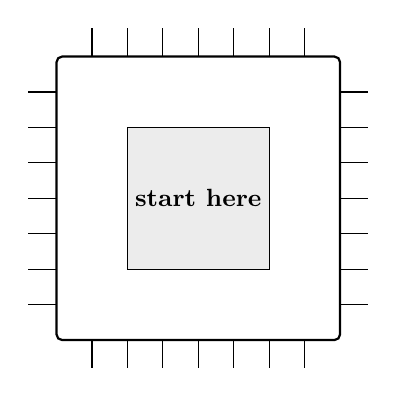
\begin{tikzpicture}[scale=0.9]
    \draw[thick,rounded corners=2pt] (0,0) rectangle (4,4);
    \foreach \i in {0.5,1,...,3.5} {
      \draw (\i,4) -- (\i,4.4); \draw (\i,0) -- (\i,-0.4);
      \draw (0,\i) -- (-0.4,\i); \draw (4,\i) -- (4.4,\i);}
    \draw[fill=gray!15] (1,1) rectangle (3,3);
    \node[font=\small\bfseries] at (2,2) {start here};
  \end{tikzpicture}
  \vfill
  {\large First edition, October 2026\par}
  \vspace{0.5em}
  {\small An unofficial study book. It is not produced or endorsed by NVIDIA.\par}
\end{titlepage}

\chapter{Preface}

\section*{Who this book is for}

This book is for someone who wants to work on computer hardware and is starting from nothing. It assumes you know high-school algebra and can read a simple program. It does \emph{not} assume you know what a voltage is, what a transistor does, or why a chip gets hot. Every idea is built from the one before it.

It was written for one specific goal: passing the hardware online assessment for NVIDIA's Ignite program, a 12-week summer internship for first- and second-year university students. But the content is the standard foundation every hardware engineer learns, so it will serve you well in your courses and in any hardware interview.

\section*{Why the assessment felt like a different subject}

Many students prepare for hardware assessments by practicing Verilog on sites like HDLBits. That is useful, but the Ignite hardware assessment mostly tests \emph{theory}: why circuits behave the way they do. Questions like these have appeared:

\begin{itemize}
  \item What is one advantage of a flip-flop over a latch?
  \item How do you build an OR gate out of a 2:1 multiplexer?
  \item If you swap the transistors in an inverter so the NMOS connects to the supply and the PMOS to ground, how does the circuit behave?
  \item If the clock frequency doubles and the supply voltage doubles, what happens to dynamic power?
  \item When temperature rises, what happens to transistor carrier mobility and to wire resistance?
  \item True or false: for the antenna rule, as long as the metal wire is safe, a small connected transistor is good.
\end{itemize}

None of these needs code. Each one needs one idea, understood well enough to apply to a small twist. This book teaches those ideas from the beginning.

\section*{What the assessment looks like}

NVIDIA does not publish the format, and it changes between years and teams. The picture below comes from candidate reports on Glassdoor and interview-preparation sites (see Appendix~\ref{app:sources}). Treat it as a guide, not a promise.

\begin{itemize}
  \item \textbf{Platform:} HackerRank, with webcam and screen recording. The link is usually open for about 48 hours; once started, the timer runs roughly 45 to 90 minutes.
  \item \textbf{Coding:} one or two easy coding problems. Reported examples include a linked-list problem, bit-manipulation problems (checking whether two addresses are on the same 4\,KB page, building a bit mask), and an XOR-of-subarrays problem.
  \item \textbf{Hardware multiple choice and true/false:} reported topics include transistors, circuits, heat sinks, ground (GND) connections, FIFOs, timing diagrams, the output of short code snippets, and every question in the list above. One hardware intern reported 15 questions in 50 minutes. Some tracks use negative marking, so a wrong guess can cost points.
  \item \textbf{After the assessment:} reported interviews ask you to build gates and flip-flops out of multiplexers, list the stages of a five-stage processor pipeline, design clock dividers, and reason about setup and hold timing.
\end{itemize}

\section*{How the reported topics map to this book}

\begin{center}
\begin{tabularx}{\linewidth}{>{\raggedright\arraybackslash}X l}
\toprule
\textbf{Reported topic} & \textbf{Where it is taught} \\
\midrule
Voltage, current, resistance, ground connections & Chapter~\ref{ch:electricity} \\
Capacitors, decoupling, signal reflections & Chapter~\ref{ch:capind} \\
Heat sinks and cooling & Chapter~\ref{ch:heat} \\
Carrier mobility and temperature & Chapters~\ref{ch:semis} and~\ref{ch:pvt} \\
Transistors, strong and weak 0 and 1, sizing & Chapter~\ref{ch:mosfet} \\
Inverters, the swapped inverter, NAND and NOR & Chapter~\ref{ch:cmos} \\
Gates built from multiplexers, XOR chains & Chapter~\ref{ch:comb} \\
Latches versus flip-flops, flip-flops from multiplexers & Chapter~\ref{ch:latch} \\
Setup, hold, timing diagrams, maximum frequency & Chapter~\ref{ch:timing} \\
Clock dividers, counters, state machines & Chapter~\ref{ch:fsm} \\
Gate and wire delay & Chapter~\ref{ch:delay} \\
Dynamic power scaling, power gating & Chapter~\ref{ch:power} \\
Wire resistance, crosstalk, bandwidth & Chapter~\ref{ch:wires} \\
Antenna rule, electromigration, latch-up & Chapter~\ref{ch:fab} \\
SRAM and DRAM & Chapter~\ref{ch:memory} \\
FIFOs, clock-domain crossing, Verilog, verification & Chapter~\ref{ch:rtl} \\
Pipelines, caches, memory access time & Chapter~\ref{ch:arch} \\
GPUs and number formats & Chapter~\ref{ch:gpu} \\
Computer arithmetic (named in the job posting) & Chapter~\ref{ch:arith} \\
Linked lists, bit manipulation, C output questions & Chapter~\ref{ch:prog} \\
Aptitude and puzzles & Chapter~\ref{ch:aptitude} \\
\bottomrule
\end{tabularx}
\end{center}

\section*{How to read this book}

Read the chapters in order. Each one builds on the last: you cannot understand why an inverter swapped upside down misbehaves (Chapter~\ref{ch:cmos}) until you understand why a transistor passes a ``weak 1'' (Chapter~\ref{ch:mosfet}), and that rests on how a transistor's channel forms (Chapter~\ref{ch:semis}).

Throughout the book you will see these boxes:

\begin{bigidea}
The one sentence to remember from a section. If you forget everything else, keep this.
\end{bigidea}

\begin{everyday}
A comparison to something you already know, such as water in pipes, to build intuition before the math.
\end{everyday}

\begin{worked}{a calculation}
A problem solved step by step, in the style of the assessment.
\end{worked}

\begin{trap}
A twist that assessment questions like to use to catch people who memorized instead of understood.
\end{trap}

\begin{onoa}
A topic or question that candidates have reported seeing on the NVIDIA assessment or in its interviews.
\end{onoa}

Every chapter ends with exercises and their answers. Try each exercise before reading the answer; the struggle is where the learning happens. Chapter~\ref{ch:exam} is a full practice assessment, Appendix~\ref{app:plan} lays out a twelve-month plan to be ready for the next application cycle, and Appendix~\ref{app:projects} lists what to learn beyond this book and the projects that make an application stand out.

\section*{A note on honesty}

The reported questions come from anonymous candidate reports, and some come from other NVIDIA hardware roles rather than Ignite itself. Where a reported question depended on a diagram that was never published, this book teaches the method for that \emph{kind} of question with its own example rather than pretending to know the original. The safest preparation is not memorizing past questions; it is understanding the ideas well enough that a new twist does not scare you.

\tableofcontents

\mainmatter

\part{Electricity, from Zero}
\chapter{Charge, Current, Voltage and Resistance}
\label{ch:electricity}

Every chip, from a calculator to a GPU, is a machine for moving tiny amounts of electric charge around. Before we can talk about transistors or logic gates, we need four words that every later chapter uses: \emph{charge}, \emph{current}, \emph{voltage} and \emph{resistance}. This chapter builds each one from scratch, then uses them to analyze simple circuits.

\section{Charge: the thing that moves}

All matter is made of atoms. An atom has a small, heavy center (the \term{nucleus}, made of protons and neutrons) surrounded by much lighter \term{electrons}. Protons carry a positive electric \term{charge}; electrons carry an equal amount of negative charge. Neutrons carry none.

Charges push and pull on each other:
\begin{itemize}
  \item Opposite charges attract (a positive and a negative pull together).
  \item Like charges repel (two negatives push apart, as do two positives).
\end{itemize}

Charge is measured in \term{coulombs} (C). One electron carries $1.6 \times 10^{-19}$\,C, so one coulomb is about $6.2 \times 10^{18}$ electrons. That is a huge number of electrons, which is why everyday electricity feels continuous rather than like individual particles.

In some materials, the outermost electrons are only loosely held by their atoms and can wander from atom to atom. These materials are \term{conductors}: metals such as copper, aluminum, gold and silver. In other materials every electron is tightly bound, so charge cannot move; these are \term{insulators}: glass, plastic, rubber, air, and silicon dioxide (which matters a lot later). Between the two are \term{semiconductors}, like silicon, whose ability to conduct can be controlled. Semiconductors get their own chapter (Chapter~\ref{ch:semis}).

\section{Current: how fast charge flows}

\term{Current} is the rate at which charge flows past a point. If 1 coulomb passes a point every second, the current is 1 \term{ampere} (A), usually shortened to ``amp.''
\[
  I = \frac{\Delta Q}{\Delta t} \qquad \text{(current = charge per unit time)}
\]

Typical sizes:
\begin{itemize}
  \item A single logic gate switching: microamps ($10^{-6}$\,A) or less.
  \item A phone charging: about 1--3\,A.
  \item A large GPU at full load: hundreds of amps, delivered at around 1\,V.
\end{itemize}

\begin{everyday}
Think of a wire as a pipe full of water. Current is how much water flows past a point each second. A wide river moving slowly and a narrow jet moving fast can carry the same flow.
\end{everyday}

\paragraph{Which direction does current flow?} By an old convention (chosen before electrons were discovered), current is drawn flowing from the positive terminal, through the circuit, to the negative terminal. Electrons, being negative, actually drift the opposite way. Engineers always use the convention, \term{conventional current}, and so does this book. The direction almost never matters for understanding a circuit, as long as you are consistent.

\section{Voltage: the push}

Charge does not move on its own; something has to push it. \term{Voltage} is that push. More precisely, voltage is the \emph{energy per unit charge} available between two points:
\[
  V = \frac{\text{energy}}{\text{charge}}, \qquad 1~\text{volt} = 1~\text{joule per coulomb}.
\]

\begin{everyday}
Voltage is like water pressure, or like height. Water flows from high pressure to low pressure, and a ball rolls from high ground to low ground. Charge flows from high voltage to low voltage. A battery is a pump that keeps one end at high pressure and the other at low pressure.
\end{everyday}

The most important fact about voltage is this:

\begin{bigidea}
Voltage is always measured \emph{between two points}. ``This wire is at 5 volts'' really means ``this wire is 5 volts higher than some reference point.''
\end{bigidea}

A height of ``100 meters'' only means something if you know where you measured from (sea level? the floor?). Voltage is the same.

\section{Ground: the reference point}
\label{sec:ground}

Because voltage is always relative, every circuit picks one node as the reference and calls it 0\,V. That node is called \term{ground}, written GND, and drawn with this symbol:
\begin{center}
\begin{circuitikz}
  \draw (0,0) -- (0,-0.5) node[ground]{};
\end{circuitikz}
\end{center}
When someone says a chip's supply is ``1.0\,V'', they mean the supply wire is 1.0\,V above that chip's ground.

Ground is not magic. It is just a wire (or, on a circuit board, a large copper plane) that everything agrees to measure from. Several practical rules follow from this.

\paragraph{Every connected device must share ground.} Suppose board A sends a ``1'' to board B as 3.3\,V. That 3.3\,V is measured relative to A's ground. If B's ground is not connected to A's ground, B has no idea what A's 3.3\,V means: the two boards have no common reference, and the signal is meaningless. This is why every cable between two devices carries a ground wire as well as the signal wires, and why a missing ground connection is one of the most common reasons a circuit ``does nothing.''

\paragraph{Current needs a return path.} Charge flows in loops. Current that leaves a power supply through the supply wire must come back through ground. If the ground path is broken, no current flows at all, just as water cannot circulate in a pipe loop with a gap in it.

\paragraph{Floating inputs.} An input that is connected to nothing (neither a voltage nor ground) is called \term{floating}. Its voltage is undefined: it drifts with stray charge and electrical noise, so a digital input reads randomly as 0 or 1. Never leave a logic input floating. Tie it to the supply or to ground, directly or through a resistor.

\paragraph{Pull-up and pull-down resistors.} A common fix for a floating input is a resistor to the supply (a \term{pull-up}) or to ground (a \term{pull-down}). In Figure~\ref{fig:pullup}, when the button is open, no current flows through the resistor, so the input sits at $\VDD$ and reads 1. When the button is pressed, the input is connected straight to ground and reads 0. The resistor limits the current that flows from the supply to ground while the button is pressed.

\begin{figure}[h]
\centering
\begin{circuitikz}
  \draw (0,3) node[vdd]{$V_{DD}$} to[R, l=$10\,\mathrm{k}\Omega$] (0,1.2)
        to[push button, l=button] (0,-0.4) node[ground]{};
  \draw (0,1.2) to[short,*-o] (2,1.2) node[right]{to logic input};
\end{circuitikz}
\caption{A pull-up resistor keeps the input at a defined 1 until the button connects it to ground.}
\label{fig:pullup}
\end{figure}

\paragraph{Ground is not perfectly 0\,V everywhere.} Real ground wires have a little resistance. When large currents flow through them, different points on ``ground'' end up at slightly different voltages. This effect, called \term{ground bounce} when it happens quickly, returns in Chapters~\ref{ch:capind} and~\ref{ch:pvt}.

\begin{onoa}
Candidates have reported questions about GND connections. Whatever the exact wording, the ideas above are the ones being tested: ground is the shared reference, current needs a return path through it, devices must share ground to communicate, and inputs must never float.
\end{onoa}

\section{Resistance and Ohm's law}

Even in a good conductor, moving charge bumps into atoms and loses energy as heat. \term{Resistance} measures how strongly a component opposes current. It is measured in \term{ohms} ($\Omega$).

For many materials, current is proportional to the voltage across them. This is \term{Ohm's law}:
\[
  \boxed{V = I R}
  \qquad\text{equivalently}\qquad I = \frac{V}{R}, \quad R = \frac{V}{I}.
\]

\begin{everyday}
Resistance is how narrow the pipe is. For the same pressure (voltage), a narrow pipe (high resistance) lets less water (current) through.
\end{everyday}

\begin{worked}{Ohm's law}
A 1\,k$\Omega$ resistor (1000 ohms) is connected across a 5\,V battery. What current flows?
\[
  I = \frac{V}{R} = \frac{5~\text{V}}{1000~\Omega} = 0.005~\text{A} = 5~\text{mA}.
\]
\end{worked}

\paragraph{What sets a wire's resistance?} A wire's resistance depends on its material and shape:
\[
  R = \rho \frac{L}{A}
\]
where $L$ is the length, $A$ is the cross-sectional area, and $\rho$ (rho) is the material's \term{resistivity}. Copper's resistivity is about $1.7 \times 10^{-8}~\Omega\cdot$m; aluminum's is about $2.7 \times 10^{-8}$. So:
\begin{itemize}
  \item A wire twice as long has twice the resistance (charge must travel further).
  \item A wire with twice the cross-section has half the resistance (more room to flow).
  \item Copper conducts better than aluminum, which is one reason modern chips use copper wiring.
\end{itemize}
Resistivity also changes with temperature; for metals it rises as they heat up. That fact is central to Chapter~\ref{ch:pvt}.

\section{Power: how fast energy is used}

When current flows through a resistance, electrical energy turns into heat. \term{Power} is the rate of energy use, measured in \term{watts} (W): one watt is one joule per second.
\[
  \boxed{P = V I}
\]
Combining with Ohm's law gives two more forms that are useful when you know only two of the three quantities:
\[
  P = I^2 R = \frac{V^2}{R}.
\]

\begin{worked}{power in a GPU}
A GPU runs at a supply of 0.9\,V and draws 400\,A. How much power does it use?
\[
  P = V I = 0.9 \times 400 = 360~\text{W}.
\]
All 360\,W ends up as heat that the cooling system must remove (Chapter~\ref{ch:heat}).
\end{worked}

\paragraph{Energy versus power.} Energy is power multiplied by time: a 360\,W GPU running for one hour uses $360 \times 3600 = 1.3$ million joules. Power is how fast you spend energy; energy is how much you spent in total. Batteries are rated in energy; chips are usually rated in power. This distinction matters in Chapter~\ref{ch:power}.

\section{Circuits: closed loops, opens and shorts}

A \term{circuit} is a closed loop through which current can flow: from a source, through components, and back. Two failure modes appear constantly:

\begin{itemize}
  \item An \term{open circuit} is a break in the loop. No current flows, no matter how high the voltage. A switch that is ``off'' is an open circuit.
  \item A \term{short circuit} is a path with (nearly) zero resistance. By Ohm's law, $I = V/R$ becomes very large. A short across a power supply can melt wires or destroy the supply.
\end{itemize}

\section{Series and parallel}

Components can be connected in two basic ways (Figure~\ref{fig:seriespar}).

\begin{figure}[h]
\centering
\begin{circuitikz}
  \draw (0,0) to[battery1, l=$V$] (0,2) to[R, l=$R_1$] (2.5,2) to[R, l=$R_2$] (2.5,0) -- (0,0);
  \node at (1.25,-0.6) {series};
  \draw (5,0) to[battery1, l=$V$] (5,2) -- (8,2);
  \draw (6.5,2) to[R, l_=$R_1$] (6.5,0);
  \draw (8,2) to[R, l=$R_2$] (8,0);
  \draw (5,0) -- (8,0);
  \node at (6.5,-0.6) {parallel};
\end{circuitikz}
\caption{Series (left): one path, same current through both. Parallel (right): two paths, same voltage across both.}
\label{fig:seriespar}
\end{figure}

\paragraph{Series.} Components in series sit one after another on a single path. The \emph{same current} flows through each, and their voltages add up. Resistances in series add:
\[
  R_{\text{series}} = R_1 + R_2 + \cdots
\]

\paragraph{Parallel.} Components in parallel connect across the same two nodes. Each has the \emph{same voltage}, and their currents add. Resistances in parallel combine as
\[
  \frac{1}{R_{\text{parallel}}} = \frac{1}{R_1} + \frac{1}{R_2} + \cdots,
  \qquad\text{and for two:}\quad R_{\text{parallel}} = \frac{R_1 R_2}{R_1 + R_2}.
\]
Parallel resistance is always \emph{smaller} than the smallest resistor, because each new path gives current another way through. Two equal resistors $R$ in parallel give $R/2$.

\begin{bigidea}
Series: same current, resistances add. Parallel: same voltage, the result is smaller than either. This exact pattern returns when we build logic gates: transistors in series make it \emph{harder} for current to flow, and transistors in parallel make it \emph{easier}.
\end{bigidea}

\begin{worked}{series and parallel together}
A 100\,$\Omega$ resistor is in series with two 200\,$\Omega$ resistors that are in parallel with each other. A 12\,V source drives the combination. Find the total current.

The parallel pair: $200 \parallel 200 = 100~\Omega$. Add the series resistor: $100 + 100 = 200~\Omega$. Current: $I = 12/200 = 0.06$\,A $= 60$\,mA. Each parallel resistor carries half of it, 30\,mA.
\end{worked}

\section{Kirchhoff's laws}

Two rules, both forms of ``nothing is created or lost,'' let you solve any circuit.

\paragraph{Kirchhoff's current law (KCL).} The total current flowing into a node equals the total current flowing out. Charge does not pile up in a wire junction.
\[
  \sum I_{\text{in}} = \sum I_{\text{out}}.
\]

\paragraph{Kirchhoff's voltage law (KVL).} Around any closed loop, the voltage rises (from sources) equal the voltage drops (across components). If you walk around a loop and return to your start, you are back at the same ``height.''
\[
  \sum V_{\text{around a loop}} = 0.
\]

\section{The voltage divider}

The single most useful small circuit is the \term{voltage divider}: two resistors in series across a voltage, with the output taken from the middle (Figure~\ref{fig:divider}).

\begin{figure}[h]
\centering
\begin{circuitikz}
  \draw (0,0) to[battery1, l=$V_{\text{in}}$] (0,3) -- (2,3) to[R, l=$R_1$] (2,1.5) to[R, l=$R_2$] (2,0) -- (0,0);
  \draw (2,1.5) to[short,*-o] (3.5,1.5) node[right]{$V_{\text{out}}$};
  \draw (0,0) node[ground]{};
\end{circuitikz}
\caption{A voltage divider.}
\label{fig:divider}
\end{figure}

The same current $I = V_{\text{in}}/(R_1 + R_2)$ flows through both resistors (they are in series). The output is the voltage across $R_2$:
\[
  \boxed{V_{\text{out}} = V_{\text{in}} \cdot \frac{R_2}{R_1 + R_2}}
\]

\begin{worked}{divider}
$V_{\text{in}} = 5$\,V, $R_1 = 3$\,k$\Omega$, $R_2 = 2$\,k$\Omega$. Then $V_{\text{out}} = 5 \times 2/(3+2) = 2$\,V.
\end{worked}

You will meet the divider idea again and again: whenever two things ``fight'' over a node, one pulling up and one pulling down, the node settles where their strengths balance. This is exactly what happens inside a logic gate when both transistors are partly on (Chapter~\ref{ch:cmos}) and inside an SRAM cell during a read (Chapter~\ref{ch:memory}).

\section{Real sources and IR drop}
\label{sec:irdrop}

A real power supply is not a perfect voltage source. The supply itself, and every wire, connector, board trace and package pin between the supply and the chip, has some resistance. Current flowing through that resistance causes a voltage drop, $V = IR$, called \term{IR drop} (I times R).

\begin{figure}[h]
\centering
\begin{circuitikz}
  \draw (0,0) to[battery1, l=$1.00$\,V regulator] (0,2.5) to[R, l=$R_{\text{path}}$, i=$I$] (4,2.5) -- (4,2.2);
  \draw (3.4,0.3) rectangle (4.6,2.2); \node at (4,1.25) {chip};
  \draw (4,0.3) -- (4,0) -- (0,0);
  \draw (0,0) node[ground]{};
\end{circuitikz}
\caption{Every bit of resistance between the regulator and the chip steals some voltage.}
\end{figure}

\begin{worked}{voltage at the chip's power pins}
A voltage regulator outputs 1.00\,V. The path to the chip has a total resistance of 0.25\,m$\Omega$ ($0.25 \times 10^{-3}~\Omega$). The chip draws 200\,A. What voltage reaches the chip?
\[
  V_{\text{drop}} = I R = 200 \times 0.00025 = 0.05~\text{V}, \qquad
  V_{\text{chip}} = 1.00 - 0.05 = 0.95~\text{V}.
\]
A quarter of a milliohm sounds like nothing, but at hundreds of amps it costs 5\% of the supply. Lower voltage makes transistors slower (Chapter~\ref{ch:pvt}), so power delivery design matters.
\end{worked}

Notice why high-power chips are hard: power is $V \times I$, and chip voltages are low (around 1\,V), so a few hundred watts means a few hundred amps. Large currents make even tiny resistances matter.

\section{Measuring voltage and current}

A \term{voltmeter} measures the voltage between two points, so it connects \emph{across} (in parallel with) the thing being measured. A good voltmeter has very high resistance so it draws almost no current and does not disturb the circuit.

An \term{ammeter} measures the current through a wire, so the wire must be broken and the meter placed \emph{in series}. A good ammeter has very low resistance so it does not add a voltage drop. Connecting an ammeter across a power supply (in parallel) creates a short circuit, a classic lab mistake.

\section{DC, AC and frequency}

A \term{DC} (direct current) signal stays at a constant value, like a battery. An \term{AC} (alternating current) signal changes over time and repeats, like the mains power in a wall outlet or a clock signal in a chip.

A repeating signal has a \term{period} $T$, the time for one full repetition, and a \term{frequency} $f$, the number of repetitions per second, measured in \term{hertz} (Hz):
\[
  f = \frac{1}{T}.
\]
A 2\,GHz clock ($2 \times 10^9$ cycles per second) has a period of $1/(2\times 10^9) = 0.5$\,ns. Square-wave signals that switch between a low and a high level also have a \term{duty cycle}: the fraction of each period spent high. A clock that is high for half its period has a 50\% duty cycle.

\section{Summary}

\begin{itemize}
  \item Charge (coulombs) is what moves. Current (amps) is how fast it flows. Voltage (volts) is the push, always measured between two points.
  \item Ground is the shared 0\,V reference. Connected devices must share ground, current returns through it, and inputs must never float.
  \item Ohm's law: $V = IR$. Power: $P = VI = I^2R = V^2/R$.
  \item Series: same current, resistances add. Parallel: same voltage, resistance falls.
  \item KCL: current in equals current out at a node. KVL: voltages around a loop sum to zero.
  \item Voltage divider: $V_{\text{out}} = V_{\text{in}} R_2/(R_1+R_2)$.
  \item IR drop: big currents through small resistances still lose voltage.
\end{itemize}

\section{Exercises}

\begin{enumerate}
  \item A 470\,$\Omega$ resistor has 2.35\,V across it. What current flows through it?
  \item Three 300\,$\Omega$ resistors are connected in parallel. What is the total resistance?
  \item A 10\,$\Omega$ resistor carries 2\,A. How much power does it dissipate?
  \item In a voltage divider, $V_{\text{in}} = 3.3$\,V, $R_1 = 10$\,k$\Omega$, $R_2 = 20$\,k$\Omega$. Find $V_{\text{out}}$.
  \item True or false: if a wire is made twice as long and twice as wide (in cross-sectional area), its resistance is unchanged.
  \item A microcontroller on board A sends signals to board B over a single wire, the signal wire, and nothing else. Board B reads random values. What is the most likely problem?
  \item A chip draws 150\,A from a 0.80\,V regulator through 0.4\,m$\Omega$ of path resistance. What voltage reaches the chip, and how much power is wasted in the path?
  \item Why is an unconnected (floating) digital input a problem, and what are two ways to fix it?
\end{enumerate}

\subsection*{Answers}
\begin{enumerate}
  \item $I = V/R = 2.35/470 = 0.005$\,A $= 5$\,mA.
  \item Three equal resistors in parallel: $300/3 = 100~\Omega$.
  \item $P = I^2R = 2^2 \times 10 = 40$\,W.
  \item $V_{\text{out}} = 3.3 \times 20/(10+20) = 2.2$\,V.
  \item True. $R = \rho L/A$: doubling $L$ doubles $R$, doubling $A$ halves it; the effects cancel.
  \item There is no shared ground. Board A's signal voltage is relative to A's ground, so without a ground wire B has no reference (and the current has no return path). Add a ground connection between the boards.
  \item Drop $= 150 \times 0.0004 = 0.06$\,V, so the chip sees $0.74$\,V. Power lost in the path $= I^2R = 150^2 \times 0.0004 = 9$\,W.
  \item Its voltage is undefined, so noise makes it read randomly as 0 or 1 (and it can also make the input circuit waste power). Fix it with a pull-up resistor to the supply or a pull-down resistor to ground, or by tying it directly to a defined level.
\end{enumerate}

\chapter{Capacitors, Inductors and the Role of Time}
\label{ch:capind}

Resistors respond instantly: change the voltage and the current changes at the same moment. Real circuits also contain components that \emph{store energy}, and stored energy takes time to fill and to drain. Those components, capacitors and inductors, are the reason every signal in a chip takes time to switch, the reason chips need dozens of small capacitors around them, and the reason fast signals on a circuit board can bounce like waves. This chapter explains all three.

\section{The capacitor}

A \term{capacitor} is two conductors (``plates'') separated by a thin insulator. Connect it to a voltage and charge flows onto the plates: positive charge piles up on one plate and an equal negative charge on the other. The insulator stops charge from crossing, so the charge stays there, held by the attraction between the plates.

The amount of charge stored is proportional to the voltage across the capacitor:
\[
  \boxed{Q = C V}
\]
The constant $C$ is the \term{capacitance}, measured in \term{farads} (F). A farad is enormous; real values are written with prefixes:

\begin{center}
\begin{tabular}{lll}
\toprule
Prefix & Value & Typical example \\
\midrule
femtofarad (fF) & $10^{-15}$\,F & the gate of one small transistor \\
picofarad (pF) & $10^{-12}$\,F & a long on-chip wire, an I/O pin \\
nanofarad (nF) & $10^{-9}$\,F & a small ceramic capacitor on a board \\
microfarad ($\mu$F) & $10^{-6}$\,F & a typical board-level decoupling capacitor \\
\bottomrule
\end{tabular}
\end{center}

For two flat plates of area $A$ separated by a gap $d$ filled with an insulator of permittivity $\varepsilon$,
\[
  C = \varepsilon \frac{A}{d}.
\]
Bigger plates hold more charge; a thinner gap holds more charge because the plates attract each other more strongly.

\begin{bigidea}
Every wire and every transistor gate in a chip \emph{is} a capacitor, whether we want it or not. A wire running next to another wire, or above the silicon, forms plates separated by insulation. A transistor's gate sits on a very thin insulator above the silicon. So every time a signal switches, some capacitance must be charged or discharged. That takes time (delay) and energy (power). Most of Chapters~\ref{ch:delay} and~\ref{ch:power} follow from this sentence.
\end{bigidea}

\begin{everyday}
A capacitor is like a water tank. The water level is the voltage; the amount of water is the charge. A wide tank (large capacitance) needs a lot of water to raise its level a little. Filling a tank through a pipe takes time, and the narrower the pipe (larger resistance), the longer it takes.
\end{everyday}

\section{Current into a capacitor}

Since $Q = CV$, changing the voltage requires moving charge, which is a current:
\[
  \boxed{I = C\,\frac{dV}{dt}}
\]
In words: the current into a capacitor equals its capacitance times how fast its voltage is changing. Two consequences:

\begin{itemize}
  \item A capacitor's voltage \emph{cannot change instantly}. An instant change would need infinite current. Voltage across a capacitor always changes smoothly.
  \item When the voltage is steady, no current flows into the capacitor. At DC, a capacitor acts like an open circuit.
\end{itemize}

\section{Energy stored in a capacitor}

A charged capacitor holds energy:
\[
  \boxed{E = \tfrac{1}{2} C V^2}
\]
The square on $V$ is important. Doubling the voltage stores four times the energy. This is why the power a chip burns when it switches grows with the \emph{square} of the supply voltage (Chapter~\ref{ch:power}).

\section{Charging through a resistor: the RC time constant}
\label{sec:rc}

Connect a capacitor, initially at 0\,V, through a resistor $R$ to a voltage $V_s$ (Figure~\ref{fig:rc}).

\begin{figure}[h]
\centering
\begin{circuitikz}
  \draw (0,0) to[battery1, l=$V_s$] (0,2.4) to[R, l=$R$, i=$I$] (3,2.4) to[C, l=$C$, v^=$V_C$] (3,0) -- (0,0);
  \draw (0,0) node[ground]{};
\end{circuitikz}
\hspace{1cm}
\begin{tikzpicture}[scale=0.9]
  \draw[->] (0,0) -- (6.2,0) node[right]{$t$};
  \draw[->] (0,0) -- (0,3.2) node[above]{$V_C$};
  \draw[dashed] (0,2.6) node[left]{$V_s$} -- (6,2.6);
  \draw[thick,blue!60!black,domain=0:6,samples=60] plot (\x,{2.6*(1-exp(-\x))});
  \draw[dotted] (1,0) node[below]{$\tau$} -- (1,{2.6*(1-exp(-1))}) -- (0,{2.6*(1-exp(-1))}) node[left]{$0.63V_s$};
  \draw[dotted] (0.69,0) -- (0.69,1.3) -- (0,1.3) node[left]{$0.5V_s$};
  \node[below] at (0.6,-0.3) {\scriptsize $0.69\tau$};
\end{tikzpicture}
\caption{Charging a capacitor through a resistor. The voltage rises quickly at first, then slows as it approaches $V_s$.}
\label{fig:rc}
\end{figure}

At the first instant the capacitor is at 0\,V, so the full $V_s$ appears across the resistor and current is large: $I = V_s/R$. As the capacitor charges, its voltage rises, the voltage left across the resistor shrinks, and the current falls. Charging slows down as it goes. The result is an exponential curve:
\[
  V_C(t) = V_s\left(1 - e^{-t/RC}\right).
\]
The product $\tau = RC$ is the \term{time constant} (ohms times farads gives seconds). These checkpoints are worth memorizing:

\begin{center}
\begin{tabular}{ll}
\toprule
Time & Capacitor voltage \\
\midrule
$0.69\,RC$ & 50\% of final value \\
$1\,RC$ & 63\% \\
$2.2\,RC$ & time to go from 10\% to 90\% (the ``rise time'') \\
$3\,RC$ & 95\% \\
$5\,RC$ & over 99\% (``fully'' charged) \\
\bottomrule
\end{tabular}
\end{center}

Discharging works the same way in reverse: a capacitor at $V_0$ discharging through $R$ follows $V_C(t) = V_0 e^{-t/RC}$ and reaches half its starting voltage after $0.69\,RC$.

\begin{worked}{an on-chip RC delay}
A transistor that behaves like a 2\,k$\Omega$ resistor drives a wire with 50\,fF of capacitance. How long until the wire reaches half the supply voltage?

$\tau = RC = 2000 \times 50\times10^{-15} = 10^{-10}$\,s $= 100$\,ps. Half-voltage takes $0.69\,\tau \approx 69$\,ps.
\end{worked}

This little calculation is the heart of all delay estimates in chip design: a transistor is a resistor, the thing it drives is a capacitor, and the delay is about $0.69\,RC$.

\section{Capacitors in series and parallel}

Capacitors combine the \emph{opposite} way from resistors:
\begin{itemize}
  \item \textbf{Parallel capacitors add}: $C = C_1 + C_2$. Side by side, they act like one capacitor with more plate area.
  \item \textbf{Series capacitors combine like parallel resistors}: $1/C = 1/C_1 + 1/C_2$. In series, the gap effectively gets wider, so capacitance falls.
\end{itemize}

\section{The inductor}

An \term{inductor} is usually a coil of wire. Current through it creates a magnetic field, and the field stores energy. Changing the current means changing the field, and the inductor fights that change by producing a voltage:
\[
  \boxed{V = L\,\frac{dI}{dt}}
\]
$L$ is the \term{inductance}, measured in \term{henries} (H). Practical values are nanohenries (nH) to microhenries ($\mu$H). The stored energy is $E = \tfrac12 L I^2$.

\begin{everyday}
An inductor is like a heavy water wheel in a pipe. Once water is moving, the wheel's momentum keeps it moving; to speed the flow up or slow it down quickly, you have to push hard. A capacitor resists sudden changes in \emph{voltage}; an inductor resists sudden changes in \emph{current}.
\end{everyday}

\paragraph{Every wire has inductance.} Coils are not the only inductors. Any loop of current, including the path from a power supply to a chip and back through ground, has some inductance. A rule of thumb is roughly 1\,nH per millimeter of a thin wire, such as the bond wires inside an older chip package. Small numbers, but chips change their current very fast.

\begin{worked}{why fast current changes are dangerous}
The power path into a chip package has an effective inductance of 10\,pH ($10 \times 10^{-12}$\,H). The chip's current jumps by 50\,A in 10\,ns when a big block starts working. What voltage appears across that inductance?
\[
  V = L\frac{dI}{dt} = 10\times10^{-12} \times \frac{50}{10\times10^{-9}} = 0.05~\text{V}.
\]
On a 0.8\,V supply, a 50\,mV dip is over 6\%. Faster current changes, or more inductance, make it worse. This dip is called \term{supply droop} or $L\,di/dt$ noise.
\end{worked}

\section{Decoupling capacitors}
\label{sec:decap}

Look at any graphics card or motherboard near the processor and you will see dozens or hundreds of tiny capacitors. They are \term{decoupling capacitors} (``decaps''), and they solve the problem in the last example.

\paragraph{The problem.} The voltage regulator that powers a chip is centimeters away. Between them sit board traces, connectors, package pins and solder balls, all with resistance and inductance. When the chip's current demand suddenly jumps, the inductance prevents the regulator's current from arriving quickly ($V = L\,dI/dt$). For a short time the chip is starved and its supply voltage dips.

\paragraph{The solution.} Put a capacitor right next to the chip's power pins, between the supply and ground. It is a small reservoir of charge, already charged to the supply voltage. When the chip suddenly needs current, the capacitor supplies it from just millimeters away, through very little inductance, while the far-away regulator catches up.

\begin{figure}[h]
\centering
\begin{circuitikz}
  \draw (0,0) to[battery1, l=regulator] (0,2.6) to[L, l=$L_{\text{path}}$] (3,2.6) to[R, l=$R_{\text{path}}$] (5.5,2.6) -- (7.2,2.6);
  \draw (5.5,2.6) to[C, l_=decap, *-*] (5.5,0);
  \draw (6.6,0.4) rectangle (7.8,2.2); \node at (7.2,1.3) {chip};
  \draw (7.2,2.6) -- (7.2,2.2);
  \draw (7.2,0.4) -- (7.2,0) -- (0,0);
  \draw (0,0) node[ground]{};
\end{circuitikz}
\caption{A decoupling capacitor next to the chip supplies sudden bursts of current that cannot get through the inductance of the long path from the regulator.}
\end{figure}

\paragraph{Why it must be close.} The capacitor only helps if \emph{its own} path to the chip has little inductance. Every millimeter of trace between the capacitor and the pin adds inductance and undoes the benefit. Real capacitors also have a little built-in inductance, called \term{ESL} (equivalent series inductance), and resistance, \term{ESR} (equivalent series resistance). Smaller capacitor packages have lower ESL.

\paragraph{Why several sizes.} Different capacitors handle different speeds of change, so designs use a ladder of them:
\begin{itemize}
  \item \textbf{Bulk capacitors} (tens to hundreds of $\mu$F) store lots of charge but have higher inductance. They cover slow changes over microseconds.
  \item \textbf{Ceramic capacitors near the chip} (roughly 0.1 to 10\,$\mu$F, in tiny packages) cover faster changes.
  \item \textbf{Capacitors inside the package and on the die itself} (on-die decap, made from transistor gates or metal layers) cover the fastest changes, within nanoseconds, because they are closest of all.
\end{itemize}

\begin{onoa}
A reported style of question asks which decoupling arrangement ``better supports rapid changes in current, and why.'' The answer to reason toward: for \emph{fast} changes, what matters is low inductance in the path, so a small, low-ESL capacitor placed as close as possible to the power pins beats a large capacitor far away. A large capacitor stores more total charge, but it cannot deliver it quickly through the inductance of a long path. Large capacitors help with slow, sustained changes.
\end{onoa}

\section{How capacitors and inductors respond to frequency}

Because a capacitor's current depends on how fast voltage changes, its effect depends on frequency. For a sine wave of frequency $f$, the capacitor's opposition to current, its \term{reactance}, is
\[
  X_C = \frac{1}{2\pi f C}.
\]
At DC ($f = 0$) this is infinite: a capacitor blocks steady current. At high frequency it becomes small: a capacitor passes fast changes. An inductor does the opposite, $X_L = 2\pi f L$: it passes DC and blocks fast changes.

A resistor followed by a capacitor to ground is a \term{low-pass filter}. Slow signals pass through unchanged; fast signals are smoothed away because the capacitor cannot charge and discharge fast enough to follow them. The boundary is the \term{cutoff frequency}
\[
  f_c = \frac{1}{2\pi R C}.
\]
Every wire on a chip is a little low-pass filter, which is why signals sent over long wires get slow and rounded.

\section{When wires become transmission lines}
\label{sec:tline}

So far we assumed a wire's voltage is the same everywhere along it. That is true when signals change slowly compared with the time a signal takes to travel down the wire. Signals do not travel instantly: on a circuit board they move at roughly half the speed of light, about 15\,cm per nanosecond. A signal that switches in 100\,ps has its edge spread over only about 1.5\,cm of board trace.

When a wire is long compared with the distance a signal edge covers, the signal travels as a wave, and the wire must be treated as a \term{transmission line}. A transmission line has a \term{characteristic impedance} $Z_0$, set by its geometry and materials. Board traces are usually designed for 50\,$\Omega$ (or 100\,$\Omega$ for a differential pair).

\paragraph{Reflections.} When a wave reaches the end of the line, some of it bounces back unless the load at the end matches $Z_0$. The fraction of the voltage that reflects is the \term{reflection coefficient}:
\[
  \boxed{\Gamma = \frac{Z_L - Z_0}{Z_L + Z_0}}
\]

\begin{center}
\begin{tabularx}{\linewidth}{>{\raggedright\arraybackslash}p{4.2cm}>{\raggedright\arraybackslash}p{1.6cm}>{\raggedright\arraybackslash}X}
\toprule
Load at the end & $\Gamma$ & What happens \\
\midrule
Matched, $Z_L = Z_0$ & 0 & no reflection; the ideal \\
Open circuit, $Z_L = \infty$ & $+1$ & everything reflects, same polarity (voltage doubles at the end) \\
Short circuit, $Z_L = 0$ & $-1$ & everything reflects, inverted \\
$Z_L > Z_0$ & positive & partial reflection, same polarity \\
$Z_L < Z_0$ & negative & partial reflection, inverted polarity \\
\bottomrule
\end{tabularx}
\end{center}

\begin{worked}{reflection from a mismatched load}
A 50\,$\Omega$ trace ends in a 25\,$\Omega$ load. What fraction of an incoming voltage step reflects, and is it inverted?
\[
  \Gamma = \frac{25 - 50}{25 + 50} = \frac{-25}{75} = -\frac13.
\]
One third of the step reflects, and since $\Gamma$ is negative, the reflection is inverted. With a 150\,$\Omega$ load instead, $\Gamma = (150-50)/(150+50) = +0.5$: half reflects, same polarity.
\end{worked}

Reflections cause \term{ringing}: the signal overshoots and wobbles before settling, which can make a receiver see extra transitions. The cure is \term{termination}: adding resistors so the line sees a matched load at the end (parallel termination) or a matched source at the start (series termination).

\section{Measuring fast signals: bandwidth}
\label{sec:probe}

A square wave is not as simple as it looks. Mathematically, a square wave of frequency $f$ is a sum of sine waves: one at $f$ (the \term{fundamental}), plus smaller ones at $3f$, $5f$, $7f$ and so on (the \term{odd harmonics}). The sharp corners come from those high harmonics.

An oscilloscope and its probe can only follow signals up to their \term{bandwidth}; above it, they act like a low-pass filter. A useful rule links bandwidth to the fastest rise time an instrument can show:
\[
  t_{\text{rise}} \approx \frac{0.35}{\text{bandwidth}}.
\]

\begin{worked}{why a square wave looks like a sine wave}
A 100\,MHz square wave is viewed with a 150\,MHz probe and scope. The fundamental (100\,MHz) passes, but the third harmonic (300\,MHz) and everything above it are filtered out. With only the fundamental left, the display shows something close to a 100\,MHz sine wave. The signal is fine; the measurement is too slow. To see the true edges you need roughly five times the signal frequency in bandwidth, or more.
\end{worked}

\section{Summary}

\begin{itemize}
  \item Capacitor: $Q = CV$, $I = C\,dV/dt$, energy $\tfrac12CV^2$. Its voltage cannot jump; it blocks DC.
  \item Every wire and transistor gate is a capacitor, so switching costs time and energy.
  \item RC charging: 50\% at $0.69RC$, 63\% at $RC$, essentially done at $5RC$.
  \item Inductor: $V = L\,dI/dt$. It resists sudden current changes. Every current loop has some inductance.
  \item Decoupling capacitors are local charge reservoirs. For fast current changes, low inductance (small and close) matters most; large capacitors handle slow changes.
  \item Long, fast wires are transmission lines. Reflection coefficient $\Gamma = (Z_L - Z_0)/(Z_L + Z_0)$; negative means inverted.
  \item Too little measurement bandwidth makes a square wave look like a sine wave.
\end{itemize}

\section{Exercises}

\begin{enumerate}
  \item A 10\,pF capacitor is charged to 1.2\,V. How much charge does it hold, and how much energy?
  \item A 2\,k$\Omega$ resistance drives a 50\,fF load. Find the time constant and the time to reach 50\%.
  \item Two 1\,$\mu$F capacitors are connected (a) in parallel and (b) in series. What is the total capacitance in each case?
  \item A current through a 1\,nH inductance changes by 2\,A in 1\,ns. What voltage appears across it?
  \item True or false: the voltage across a capacitor can change instantly if the current is large enough.
  \item You can place either a 100\,$\mu$F capacitor 10\,cm from a chip or a 0.1\,$\mu$F capacitor right next to its power pins. Which better handles a sudden current step lasting a few nanoseconds? Why?
  \item A 50\,$\Omega$ line drives a 150\,$\Omega$ load. Find the reflection coefficient. Is the reflection inverted?
  \item A 200\,MHz clock looks like a sine wave on a 250\,MHz oscilloscope. Is the clock broken?
\end{enumerate}

\subsection*{Answers}
\begin{enumerate}
  \item $Q = CV = 10\times10^{-12}\times1.2 = 12$\,pC. $E = \tfrac12CV^2 = 0.5\times10\times10^{-12}\times1.44 = 7.2$\,pJ.
  \item $\tau = 2000 \times 50\times10^{-15} = 100$\,ps. 50\% at $0.69\tau \approx 69$\,ps.
  \item (a) 2\,$\mu$F. (b) 0.5\,$\mu$F.
  \item $V = L\,dI/dt = 10^{-9} \times 2/10^{-9} = 2$\,V.
  \item False. In any real circuit current is finite, so the voltage changes at a finite rate; it changes quickly with large current, but never instantly.
  \item The small capacitor next to the pins. A fast current step is limited by inductance, and the capacitor that is 10\,cm away sits behind a lot of path inductance. The big capacitor helps only with slower, longer changes.
  \item $\Gamma = (150-50)/(150+50) = 0.5$. Positive, so not inverted.
  \item Probably not. The scope's bandwidth removes the third harmonic (600\,MHz) and above, so only the 200\,MHz fundamental is displayed, which is a sine wave. Use a faster scope and probe to judge the real edges.
\end{enumerate}

\chapter{Heat: Where Every Watt Ends Up}
\label{ch:heat}

A chip does useful work, but physically, all the electrical energy it consumes turns into heat. A GPU drawing 700\,W is, from the room's point of view, a 700\,W heater. Getting that heat out without letting the chip overheat is a major part of hardware engineering, and candidates have reported assessment questions on heat sinks. This chapter explains how heat moves, how to calculate a chip's temperature, and why heat sinks are built the way they are.

\section{Every watt becomes heat}

Energy is never destroyed, only converted. When current flows through the resistance of wires and transistors, electrical energy becomes heat (Chapter~\ref{ch:electricity}). Charging and discharging capacitance also turns energy into heat in the transistors that do the charging (Chapter~\ref{ch:power}). The chip stores almost none of this energy, so in steady operation:
\[
  \text{heat produced per second} = \text{electrical power consumed}.
\]

What makes chips hard to cool is not just total power but \term{power density}: power per unit area. A large GPU die is roughly 8\,cm$^2$. At 700\,W that is close to 90\,W/cm$^2$, many times the power density of a kitchen stove burner, concentrated in a sliver of silicon smaller than a postage stamp.

\section{Why temperature matters}

Silicon chips are typically allowed to run up to a maximum \term{junction temperature} (the temperature of the transistors themselves) of around 100 to 110\,\textdegree C, depending on the product. Staying below that limit matters because temperature affects nearly everything:

\begin{itemize}
  \item \textbf{Leakage power rises steeply with temperature} (Chapter~\ref{ch:power}). Hotter chips waste more power even when idle, which makes them hotter still.
  \item \textbf{Speed changes.} In most conditions transistors and wires get slower when hot (Chapter~\ref{ch:pvt}).
  \item \textbf{Aging speeds up.} Wear-out mechanisms such as electromigration (Chapter~\ref{ch:fab}) accelerate strongly with temperature. A common rule of thumb is that many failure rates roughly double for every 10\,\textdegree C rise.
\end{itemize}

\section{The three ways heat moves}

\begin{itemize}
  \item \term{Conduction}: heat flows through a solid (or still fluid) from hot to cold, passed along by vibrating atoms and moving electrons. This is how heat gets from the transistors, through the silicon and metal, to the heat sink.
  \item \term{Convection}: a moving fluid (air or liquid) picks up heat from a surface and carries it away. This is how a heat sink hands its heat to the air. A fan makes it \emph{forced} convection, which is far more effective than air drifting on its own (\emph{natural} convection).
  \item \term{Radiation}: hot objects emit infrared light. For chips at normal temperatures this is a small effect, and we will ignore it.
\end{itemize}

\section{Thermal resistance: Ohm's law for heat}

Heat flow behaves just like current in a circuit, which gives us a powerful shortcut:

\begin{center}
\begin{tabular}{ll}
\toprule
Electrical & Thermal \\
\midrule
Current $I$ (A) & Heat flow $P$ (W) \\
Voltage difference $V$ (V) & Temperature difference $\Delta T$ (\textdegree C) \\
Resistance $R$ ($\Omega$) & Thermal resistance $\theta$ (\textdegree C/W) \\
$V = IR$ & $\Delta T = P\,\theta$ \\
\bottomrule
\end{tabular}
\end{center}

\begin{bigidea}
Temperature rise equals power times thermal resistance: $\Delta T = P\,\theta$. A thermal resistance of 0.2\,\textdegree C/W means every watt flowing through it raises the temperature difference across it by 0.2\,\textdegree C.
\end{bigidea}

Heat leaving a chip passes through a chain of layers, one after another, so their thermal resistances add in series exactly like resistors (Figure~\ref{fig:thermalstack}).

\begin{figure}[h]
\centering
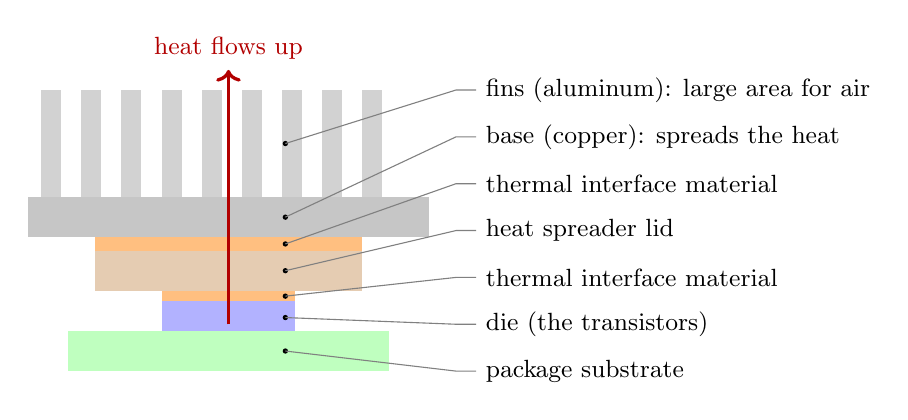
\begin{tikzpicture}[scale=0.85]
  % fins and base
  \foreach \x in {0.2,0.8,...,5.6} \fill[gray!35] (\x,3.4) rectangle (\x+0.3,5.0);
  \fill[gray!45] (0,2.8) rectangle (6,3.4);
  \fill[orange!50] (1.0,2.6) rectangle (5.0,2.8);
  \fill[brown!40] (1,2.0) rectangle (5,2.6);
  \fill[orange!50] (2,1.85) rectangle (4,2.0);
  \fill[blue!30] (2,1.4) rectangle (4,1.85);
  \fill[green!25] (0.6,0.8) rectangle (5.4,1.4);
  \draw[->,very thick,red!70!black] (3,1.5) -- (3,5.3) node[above]{\small heat flows up};
  % labels with leader lines
  \foreach \y/\ly/\t in {4.2/5.0/{fins (aluminum): large area for air},
                     3.1/4.3/{base (copper): spreads the heat},
                     2.7/3.6/{thermal interface material},
                     2.3/2.9/{heat spreader lid},
                     1.92/2.2/{thermal interface material},
                     1.6/1.5/{die (the transistors)},
                     1.1/0.8/{package substrate}} {
    \fill[black] (3.85,\y) circle (0.04);
    \draw[gray] (3.85,\y) -- (6.4,\ly) -- (6.7,\ly);
    \node[anchor=west,font=\small] at (6.7,\ly) {\t};}
\end{tikzpicture}
\caption{The path heat takes from the transistors to the air. Each layer adds thermal resistance.}
\label{fig:thermalstack}
\end{figure}

The standard names are:
\begin{itemize}
  \item $\theta_{jc}$: junction to case (from the transistors, through the die and lid).
  \item $\theta_{cs}$: case to sink (through the thermal interface material).
  \item $\theta_{sa}$: sink to ambient (from the heat sink into the surrounding air).
\end{itemize}
\[
  T_{\text{junction}} = T_{\text{ambient}} + P\,(\theta_{jc} + \theta_{cs} + \theta_{sa}).
\]

\begin{worked}{junction temperature}
A 300\,W chip has $\theta_{jc} = 0.05$, $\theta_{cs} = 0.03$ and $\theta_{sa} = 0.10$\,\textdegree C/W. The air entering the heat sink is at 35\,\textdegree C. What is the junction temperature?

Total thermal resistance: $0.05 + 0.03 + 0.10 = 0.18$\,\textdegree C/W. Temperature rise: $300 \times 0.18 = 54$\,\textdegree C. Junction temperature: $35 + 54 = 89$\,\textdegree C.
\end{worked}

\begin{worked}{sizing a heat sink}
The same chip must stay below 95\,\textdegree C with 40\,\textdegree C air. What is the largest $\theta_{sa}$ the heat sink may have?

Allowed rise: $95 - 40 = 55$\,\textdegree C. Allowed total resistance: $55/300 \approx 0.183$\,\textdegree C/W. Subtract the fixed parts: $0.183 - 0.05 - 0.03 = 0.103$\,\textdegree C/W. The heat sink and fan must achieve about 0.10\,\textdegree C/W or better.
\end{worked}

\section{Conduction and materials}

How well a material conducts heat is its \term{thermal conductivity} $k$, in W/(m$\cdot$K). A slab of thickness $L$ and area $A$ has thermal resistance
\[
  \theta = \frac{L}{k A},
\]
the same form as electrical resistance $R = \rho L / A$. Thin, wide layers of high-$k$ material are best.

\begin{center}
\begin{tabular}{lrl}
\toprule
Material & $k$ (W/(m$\cdot$K)), approx. & Notes \\
\midrule
Copper & 400 & excellent conductor; heavy, costly \\
Aluminum & 205--237 & about half of copper; light, cheap, easy to shape \\
Silicon & 150 & the die itself conducts well \\
Thermal paste & 1--10 & far worse than metal, but far better than air \\
Water (still) & 0.6 & poor conductor when not moving \\
Air (still) & 0.026 & a very good insulator \\
\bottomrule
\end{tabular}
\end{center}

\section{Heat sinks}

A heat sink has one job: take heat that is concentrated in a small area and spread it over a very large surface that moving air can touch. Its design follows from the two steps it performs.

\paragraph{Spreading (conduction).} The base sits on the chip and must carry heat sideways and upward quickly, without large temperature differences across it. This calls for high thermal conductivity, which is why bases are often copper. Many heat sinks also use \term{heat pipes} or \term{vapor chambers}: sealed copper tubes or plates containing a little liquid. The liquid boils at the hot end, the vapor rushes to the cold end and condenses, and the liquid wicks back. Moving heat by evaporation and condensation gives an effective conductivity far higher than solid copper.

\paragraph{Dumping (convection).} The \term{fins} give a large surface area to the air. Convection is roughly proportional to surface area, so more fins (or taller, thinner ones) remove more heat, up to the point where fins are so close that air cannot flow between them. A fan forces air through the fins and greatly lowers $\theta_{sa}$.

\paragraph{Why combine copper and aluminum?} Copper conducts heat about twice as well as aluminum, but it is about 3.3 times as dense (8.96 versus 2.70\,g/cm$^3$), costs more, and is harder to form into thin fins. A heat sink made entirely of copper would be very heavy and expensive. So a common design uses copper where heat is concentrated and conduction matters most (the base and heat pipes), and aluminum where large area matters most (the fins). Each metal goes where its strength counts.

\begin{onoa}
Candidates have reported multiple-choice questions on heat sinks. The ideas to have ready: fins increase surface area for convection; fans lower the sink-to-air thermal resistance; copper conducts better but is heavier and costlier than aluminum, so the two are combined; heat pipes move heat by phase change; and thermal paste fills air gaps.
\end{onoa}

\section{Thermal interface materials}

Two metal surfaces that look flat are rough at the microscopic scale. Pressed together, they touch only at high points, leaving tiny gaps filled with air, and air is an excellent insulator. A \term{thermal interface material} (TIM), such as thermal paste, a pad, or a soldered metal layer, fills those gaps.

TIM conducts heat much worse than metal, so it should be as thin as possible: just enough to fill the gaps. Too much paste adds thermal resistance instead of removing it.

\section{Air versus liquid cooling}

The heat a moving fluid carries away is
\[
  P = \dot m\, c\, \Delta T,
\]
where $\dot m$ is the mass flow rate (kg/s), $c$ the \term{specific heat} (energy to warm 1\,kg by 1\,\textdegree C), and $\Delta T$ how much the fluid warms up. Water's specific heat is about 4.18\,J/(g$\cdot$K), about four times air's (about 1.0), and water is roughly 800 times denser. Per unit volume, water carries several thousand times more heat per degree than air.

\begin{worked}{removing 1000\,W}
How much water, and how much air, must flow to carry away 1000\,W while warming by 10\,\textdegree C?

Water: $\dot m = 1000/(4180 \times 10) \approx 0.024$\,kg/s, about 1.4 liters per minute: a gentle trickle.

Air: $\dot m = 1000/(1005 \times 10) \approx 0.10$\,kg/s. At about 1.2\,kg/m$^3$, that is about 0.083\,m$^3$/s, or 83 liters every second: a powerful fan.
\end{worked}

This is why the highest-power data-center GPU systems are increasingly liquid cooled: air simply cannot move enough heat through a small space.

\section{Thermal throttling and runaway}

Chips contain on-die temperature sensors. When the temperature approaches the limit, power-management firmware lowers the clock frequency and supply voltage. Because dynamic power is proportional to $V^2 f$ (Chapter~\ref{ch:power}), even a modest reduction cuts power, and therefore heat, sharply. This is \term{thermal throttling}.

\term{Thermal runaway} is the dangerous loop in the other direction: higher temperature raises leakage power, which raises temperature, which raises leakage further. A cooling system must have enough margin that this loop settles instead of running away.

\section{Summary}

\begin{itemize}
  \item All the power a chip consumes becomes heat; power density is what makes cooling hard.
  \item Heat moves by conduction, convection and radiation (the last is minor for chips).
  \item $\Delta T = P\,\theta$; thermal resistances in the heat path add in series.
  \item Heat sinks spread heat (conduction: copper base, heat pipes) and dump it (convection: large fin area, fans).
  \item Copper conducts better but is heavy and costly; aluminum is light and cheap; good designs combine them.
  \item TIM replaces insulating air gaps; it should be thin.
  \item Liquid carries far more heat per volume than air.
\end{itemize}

\section{Exercises}

\begin{enumerate}
  \item A 250\,W chip has a total junction-to-ambient thermal resistance of 0.2\,\textdegree C/W in 25\,\textdegree C air. Find its junction temperature.
  \item A 400\,W chip must stay below 95\,\textdegree C in 40\,\textdegree C air. What is the maximum total thermal resistance allowed?
  \item Why do many heat sinks use a copper base with aluminum fins rather than one metal throughout?
  \item Why is thermal paste needed between a chip and its heat sink, and why should the layer be thin?
  \item True or false: adding fins to a heat sink increases its thermal resistance.
  \item A chip is overheating. Its firmware lowers the supply voltage by 10\% and the clock frequency by 10\%. By roughly what percentage does dynamic power fall?
  \item Explain thermal runaway in one or two sentences.
\end{enumerate}

\subsection*{Answers}
\begin{enumerate}
  \item $T_j = 25 + 250 \times 0.2 = 75$\,\textdegree C.
  \item $(95 - 40)/400 = 0.1375$\,\textdegree C/W.
  \item Copper conducts heat about twice as well, which matters most where heat is concentrated (the base). But copper is about 3.3 times denser and more expensive, so the large fin area is made of light, cheap aluminum. Each material is used where it helps most.
  \item Microscopic roughness leaves air gaps, and air insulates. Paste fills the gaps. Paste conducts much worse than metal, so a thick layer adds resistance; it should be just thick enough to fill the gaps.
  \item False. Fins add surface area for convection, which lowers the sink-to-air thermal resistance.
  \item Power scales with $V^2 f$: $0.9^2 \times 0.9 = 0.729$, so power falls by about 27\%.
  \item Higher temperature increases leakage power, which produces more heat and raises temperature further. If cooling cannot keep up, the loop keeps escalating.
\end{enumerate}


\part{Semiconductors and Transistors}
\chapter{Semiconductors: Making Silicon Useful}
\label{ch:semis}

A computer needs billions of switches that can be flipped by an electrical signal, with no moving parts, billions of times per second. Metals cannot do this: they always conduct. Insulators cannot either: they never conduct. We need a material whose ability to conduct can be \emph{controlled}. That material is a semiconductor, almost always silicon. This chapter explains what makes silicon special, how ``doping'' turns it into a building material, and how temperature changes its behavior, which is one of the questions from the assessment.

\section{Electrons that can and cannot move}

Recall from Chapter~\ref{ch:electricity} that a material conducts when some of its electrons are free to move. Whether they are free depends on how tightly atoms hold their outermost electrons, called \term{valence electrons}.

\begin{itemize}
  \item In a \term{metal}, valence electrons are not tied to any one atom. They form a ``sea'' of free electrons that drifts easily when a voltage is applied. Metals conduct very well.
  \item In an \term{insulator}, every electron is locked in a chemical bond. Breaking one free takes a lot of energy, so almost none are free.
  \item In a \term{semiconductor}, electrons are bound, but not very tightly. A small amount of energy, such as heat at room temperature, frees a few of them.
\end{itemize}

Physicists describe this with an energy gap, the \term{band gap}: the minimum energy needed to free a bound electron. Silicon's band gap is about 1.12 electron-volts (eV). Silicon dioxide, a good insulator, has a gap of about 9\,eV. Metals have no gap at all.

\section{The silicon crystal}

A silicon atom has four valence electrons. In a crystal, each silicon atom shares one electron with each of four neighbors, forming four bonds (Figure~\ref{fig:silattice}). Every electron is used in a bond, so at very low temperature pure silicon is an insulator.

At room temperature, atoms vibrate. Occasionally the vibration shakes an electron out of its bond. Two things result:
\begin{enumerate}
  \item A \term{free electron} that can wander through the crystal and carry current.
  \item A \term{hole}: the empty spot where the electron used to be.
\end{enumerate}
In pure silicon at room temperature, fewer than one atom in a trillion has lost an electron this way, so pure silicon conducts very poorly.

\begin{figure}[h]
\centering
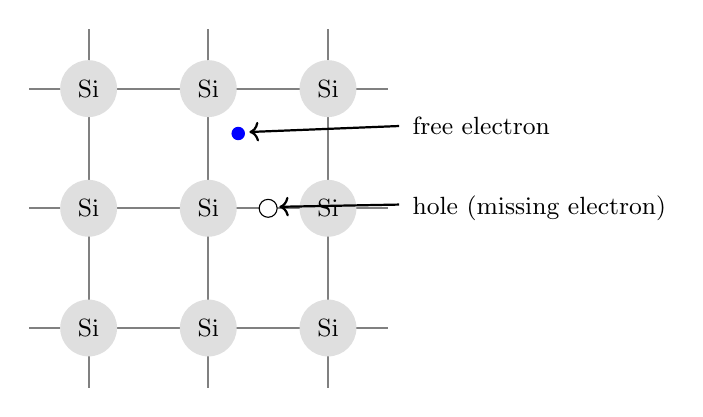
\begin{tikzpicture}[scale=0.95]
  \foreach \x in {0,1.6,3.2} \foreach \y in {0,1.6,3.2} {
    \draw[thick,gray] (\x,\y) -- ++(0.8,0); \draw[thick,gray] (\x,\y) -- ++(-0.8,0);
    \draw[thick,gray] (\x,\y) -- ++(0,0.8); \draw[thick,gray] (\x,\y) -- ++(0,-0.8);
    \fill[gray!25] (\x,\y) circle (0.38); \node at (\x,\y) {\small Si};}
  \fill[white] (2.4,1.6) circle (0.12); \draw (2.4,1.6) circle (0.12);
  \node[right,font=\small] at (4.2,1.6) {hole (missing electron)};
  \draw[->,thick] (4.15,1.65) -- (2.55,1.62);
  \fill[blue] (2.0,2.6) circle (0.09);
  \node[right,font=\small] at (4.2,2.7) {free electron};
  \draw[->,thick] (4.15,2.7) -- (2.15,2.62);
\end{tikzpicture}
\caption{Silicon atoms each share four bonds. Heat occasionally frees an electron, leaving a hole behind.}
\label{fig:silattice}
\end{figure}

\section{Holes: the missing electron that moves}

A hole is not a particle; it is the absence of an electron. But it behaves like a positive charge that can move. Here is why. If a neighboring bonded electron hops into the hole, the hole has effectively moved to where that electron came from. Under a voltage, electrons hop one way and the hole travels the other way, exactly as a positive charge would.

\begin{everyday}
Picture a row of full seats in a theater with one empty seat. When the person next to the empty seat slides over, the empty seat moves one place the other way. Keep sliding and the empty seat ``travels'' down the row, even though only people moved. The hole is the empty seat.
\end{everyday}

So a semiconductor has \emph{two} kinds of charge carriers: negative electrons and positive holes. This is the key to building two kinds of transistors.

\section{Doping: controlling the carriers}
\label{sec:doping}

Pure silicon has too few carriers to be useful. \term{Doping} adds a tiny, carefully controlled amount of another element, typically a few atoms per million or less, and changes conductivity enormously.

\paragraph{n-type silicon.} Add atoms with \emph{five} valence electrons, such as phosphorus or arsenic. Four electrons bond with silicon neighbors; the fifth has nothing to bond with and is freed easily. The silicon now has many free electrons, which carry negative charge, so it is called \term{n-type}. Electrons are its \term{majority carriers}; holes are \term{minority carriers}.

\paragraph{p-type silicon.} Add atoms with \emph{three} valence electrons, such as boron. One bond is left incomplete, creating a hole. The silicon now has many holes, which act as positive carriers, so it is called \term{p-type}. Holes are its majority carriers.

\begin{remember}
\textbf{n}-type: extra \textbf{n}egative carriers (electrons), from 5-electron dopants like phosphorus.\\
\textbf{p}-type: extra \textbf{p}ositive carriers (holes), from 3-electron dopants like boron.\\
A doped crystal is still electrically neutral overall: every extra free electron is balanced by a positive dopant nucleus, and every hole by a negative one.
\end{remember}

Chip designers write \term{n+} or \term{p+} for heavily doped regions (which conduct well and form transistor terminals), and speak of an \term{n-well}: a region of n-type silicon built into a p-type wafer so that both kinds of transistor can live on the same chip (Chapter~\ref{ch:mosfet}).

\section{How carriers move: drift, diffusion and mobility}

Carriers move for two reasons:
\begin{itemize}
  \item \term{Drift}: an electric field (a voltage across a distance) pushes them. Electrons drift toward the higher voltage; holes toward the lower.
  \item \term{Diffusion}: carriers spread from where they are crowded to where they are sparse, like a drop of ink spreading in water. No voltage is needed.
\end{itemize}

How fast a carrier drifts in a given field is its \term{mobility}, written $\mu$ (mu):
\[
  v_{\text{drift}} = \mu\,E,
\]
where $E$ is the electric field (volts per meter). Higher mobility means faster carriers, more current, and faster transistors.

\begin{center}
\begin{tabular}{ll}
\toprule
Carrier in silicon & Mobility (lightly doped, room temperature) \\
\midrule
Electrons & about 1400\,cm$^2$/(V$\cdot$s) \\
Holes & about 450\,cm$^2$/(V$\cdot$s) \\
\bottomrule
\end{tabular}
\end{center}

\begin{bigidea}
Electrons are about two to three times more mobile than holes. Holes move only by electrons hopping from bond to bond, which is slower than a free electron's travel. This single fact is why PMOS transistors (which use holes) are weaker than NMOS transistors (which use electrons), and why PMOS transistors are usually drawn about twice as wide (Chapter~\ref{ch:mosfet}).
\end{bigidea}

At very high fields, carriers stop speeding up; their velocity levels off at roughly $10^7$\,cm/s. This \term{velocity saturation} matters in modern, very short transistors.

\section{What heat does to semiconductors and to metal}
\label{sec:tempmobility}

Temperature changes conduction in two competing ways, and semiconductors and metals respond differently.

\paragraph{Effect 1: more scattering, so lower mobility.} A hotter crystal vibrates more. Carriers moving through it collide with the vibrating atoms more often (these vibrations are called \term{phonons}, and the collisions \term{phonon scattering}). More collisions mean carriers cannot build up speed, so \textbf{mobility decreases as temperature increases}. Transistors therefore carry less current and get slower.

\paragraph{Effect 2: more carriers.} Heat also frees more electrons from bonds. In pure silicon the number of free carriers rises very steeply (exponentially) with temperature. In a transistor that is supposed to be off, those extra carriers show up as \term{leakage current}, which grows rapidly when the chip is hot.

\paragraph{Metals.} A metal's free electrons are already all free; heat does not add more. Only effect 1 applies: more vibration means more scattering. So \textbf{metal resistance increases with temperature}. For copper, resistance rises by about 0.4\% per \textdegree C, so a wire 100\,\textdegree C hotter has roughly 40\% more resistance.

\begin{onoa}
A reported question asked how carrier mobility and wire resistance change when temperature increases. Answer: \textbf{carrier mobility decreases} (more phonon scattering), so transistors drive less current; \textbf{wire resistance increases} (also more scattering), so wires get slower. Both effects make the circuit slower at high temperature. Chapter~\ref{ch:pvt} adds one twist: the transistor's threshold voltage also drops when hot, which pushes the other way and, at low supply voltages, can win.
\end{onoa}

\section{The PN junction and the diode}
\label{sec:pn}

Something important happens where p-type and n-type silicon meet, a \term{PN junction}.

Near the boundary, free electrons from the n side diffuse into the p side and fill holes; holes from the p side diffuse into the n side. Carriers near the boundary cancel out, leaving a thin \term{depletion region} with no free carriers. The dopant atoms left behind are charged (positive on the n side, negative on the p side), creating a built-in electric field that stops further diffusion. The built-in voltage is a few tenths of a volt.

This structure is a \term{diode}, a one-way valve for current:
\begin{itemize}
  \item \term{Forward bias} (p side more positive than n side): the applied voltage fights the built-in barrier, the depletion region shrinks, and current flows easily once the voltage exceeds about 0.6--0.7\,V for silicon. Current grows exponentially with voltage:
  \[
    I = I_S\left(e^{V/V_T} - 1\right), \qquad V_T = \frac{kT}{q} \approx 26~\text{mV at room temperature}.
  \]
  \item \term{Reverse bias} (n side more positive): the barrier grows, the depletion region widens, and only a tiny leakage current flows. At a large enough reverse voltage the junction \term{breaks down} and conducts heavily.
\end{itemize}

\begin{center}
\begin{circuitikz}
  \draw (0,0) node[left]{anode (p)} to[D] (2.5,0) node[right]{cathode (n)};
  \node[font=\small] at (1.25,-0.8) {current flows easily from anode to cathode};
\end{circuitikz}
\end{center}

Diodes matter to a digital designer in three ways:
\begin{itemize}
  \item Every transistor's source and drain form PN junctions with the silicon beneath them. These junctions must always stay reverse biased, which is why the p-type body under NMOS transistors is tied to ground and the n-well under PMOS transistors is tied to the supply (Chapter~\ref{ch:mosfet}).
  \item Reverse-biased junctions leak a little, adding to leakage power.
  \item Diodes are deliberately added to protect circuits: from static electricity (ESD protection) and from charge collected during manufacturing (antenna diodes, Chapter~\ref{ch:fab}).
\end{itemize}

\section{Silicon dioxide: silicon's perfect partner}

Silicon has a lucky property: heat it in oxygen and it grows a layer of \term{silicon dioxide} (SiO$_2$), essentially glass, which is an excellent insulator and bonds cleanly to the silicon. A thin layer of insulator on silicon is exactly what a transistor's gate needs (next chapter). In the most advanced processes, the gate insulator is so thin that designers switched to materials with higher permittivity (``high-$k$'' dielectrics such as hafnium oxide), which give the same capacitance with a physically thicker, less leaky layer.

\section{Summary}

\begin{itemize}
  \item Semiconductors sit between conductors and insulators: a little energy frees their electrons.
  \item Freeing an electron leaves a hole, which behaves like a moving positive charge.
  \item Doping controls carriers: phosphorus or arsenic makes n-type (electrons); boron makes p-type (holes).
  \item Mobility measures how fast carriers drift. Electrons are 2--3 times more mobile than holes, so NMOS is stronger than PMOS.
  \item Heat lowers mobility (transistors slow down), raises metal resistance (wires slow down), and sharply raises leakage.
  \item A PN junction is a diode: it conducts in forward bias and blocks (with slight leakage) in reverse bias.
\end{itemize}

\section{Exercises}

\begin{enumerate}
  \item Why is pure silicon a poor conductor at room temperature?
  \item Which dopant makes n-type silicon, boron or phosphorus? Explain using valence electrons.
  \item What are the majority carriers in p-type silicon?
  \item Electron mobility is about three times hole mobility. Name one consequence for chip design.
  \item As temperature rises, what happens to (a) carrier mobility, (b) copper wire resistance, (c) transistor leakage current?
  \item True or false: a hole is a positively charged particle, like a proton, that moves through the crystal.
  \item A silicon diode has 0.7\,V across it with the p side positive. Is it conducting? What if the polarity is reversed?
  \item Why is the p-type body under NMOS transistors connected to ground?
\end{enumerate}

\subsection*{Answers}
\begin{enumerate}
  \item All its valence electrons are locked in bonds; at room temperature heat frees only a tiny number, so there are very few carriers.
  \item Phosphorus. It has five valence electrons; four bond with silicon neighbors and the fifth is easily freed, adding free electrons.
  \item Holes.
  \item PMOS transistors are weaker for the same size, so they are made wider (about 2--3 times) to match NMOS strength; also, gate designs prefer to put PMOS in parallel rather than in series (Chapter~\ref{ch:cmos}).
  \item (a) Decreases. (b) Increases. (c) Increases, steeply.
  \item False. A hole is the absence of an electron in a bond. It behaves like a positive charge because neighboring electrons hop into it, making the vacancy move.
  \item Yes, it is forward biased and conducting. Reversed, it blocks current except for a tiny leakage.
  \item To keep the PN junctions between the n+ source/drain regions and the p-type body reverse biased (the body is at the lowest voltage), so they do not conduct.
\end{enumerate}

\chapter{The MOSFET: A Switch Controlled by Voltage}
\label{ch:mosfet}

Every digital chip is built from one device repeated billions of times: the \term{MOSFET}, short for metal--oxide--semiconductor field-effect transistor. If you understand this chapter, a surprising number of assessment questions become easy, including the swapped inverter and every question about ``strong'' and ``weak'' logic levels.

\section{What we want}

We want a switch with three wires. Two wires are the ends of the switch, and current flows between them when the switch is closed. The third wire controls the switch: a high voltage on it closes the switch, a low voltage opens it. Crucially, the control wire should not draw any steady current, so one switch can control many others without being drained.

The MOSFET does exactly this. Its terminals are:
\begin{itemize}
  \item the \term{gate} (G): the control input;
  \item the \term{source} (S) and \term{drain} (D): the two ends of the switch;
  \item the \term{body} (B), also called the bulk or substrate: the silicon underneath, usually tied to a fixed voltage and often not drawn.
\end{itemize}

\section{Inside an NMOS transistor}

Figure~\ref{fig:nmoscross} shows a slice through an NMOS transistor. Starting from p-type silicon (the body), two heavily doped n+ regions are formed: the source and the drain. Between them, on the surface, sits a very thin layer of insulating oxide, and on top of that the gate electrode. The distance from source to drain is the channel \term{length} $L$; the distance into the page is the channel \term{width} $W$.

\begin{figure}[h]
\centering
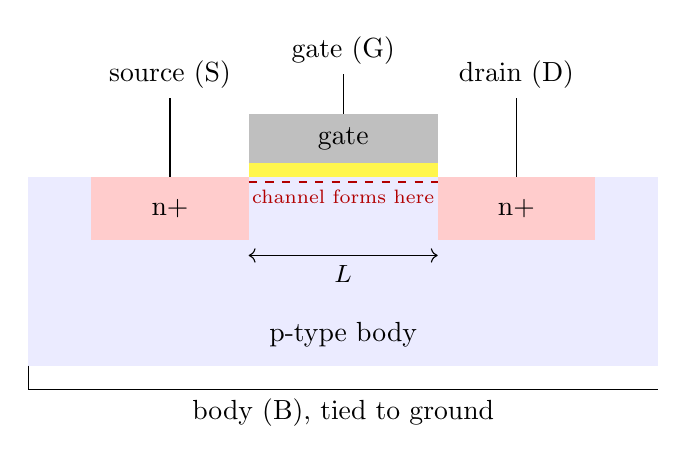
\begin{tikzpicture}[scale=1.0]
  \fill[blue!8] (0,0) rectangle (8,2.4); \node at (4,0.4) {p-type body};
  \fill[red!20] (0.8,1.6) rectangle (2.8,2.4); \node at (1.8,2.0) {n+};
  \fill[red!20] (5.2,1.6) rectangle (7.2,2.4); \node at (6.2,2.0) {n+};
  \fill[yellow!70] (2.8,2.4) rectangle (5.2,2.58);
  \fill[gray!50] (2.8,2.58) rectangle (5.2,3.2); \node at (4,2.88) {gate};
  \draw (1.8,2.4) -- (1.8,3.4) node[above]{source (S)};
  \draw (6.2,2.4) -- (6.2,3.4) node[above]{drain (D)};
  \draw (4,3.2) -- (4,3.7) node[above]{gate (G)};
  \draw (0,0) -- (0,-0.3) -- (8,-0.3); \node[below] at (4,-0.3) {body (B), tied to ground};
  \draw[<->] (2.8,1.4) -- node[below,font=\small]{$L$} (5.2,1.4);
  \draw[dashed,red!70!black,thick] (2.8,2.33) -- (5.2,2.33);
  \node[font=\scriptsize,red!70!black] at (4,2.15) {channel forms here};
\end{tikzpicture}
\caption{Cross-section of an NMOS transistor. The yellow strip under the gate is the thin insulating oxide.}
\label{fig:nmoscross}
\end{figure}

\section{How the channel forms}

With the gate at 0\,V, look at the path from source to drain: n+ silicon, then p-type body, then n+ silicon. That is two PN junctions back to back (Chapter~\ref{ch:semis}), and whichever way you push current, one of them is reverse biased. No current flows. The switch is \emph{open}.

Now raise the gate voltage. The gate, the oxide and the silicon form a capacitor. A positive gate attracts negative charge to the silicon surface just under the oxide: it pushes holes away and pulls in electrons. Once the gate voltage is high enough, electrons outnumber holes in a thin surface layer. That layer has effectively become n-type: an \term{inversion layer}, or \term{channel}. Now there is a continuous n-type path from source to drain, and current can flow. The switch is \emph{closed}.

The gate-to-source voltage needed to form the channel is the \term{threshold voltage}, $\Vt$. In modern chips it is typically 0.2 to 0.5\,V, with supply voltages around 0.7 to 1.2\,V.

\begin{bigidea}
An NMOS transistor is on when its gate is higher than its source by more than the threshold voltage: $V_{GS} > \Vtn$. The higher the gate goes above that, the more electrons fill the channel, the lower its resistance, and the more current it carries.
\end{bigidea}

\paragraph{The gate draws no steady current.} The gate sits on an insulator, so no DC current flows into it. The only current is the brief flow needed to charge or discharge the gate capacitance when its voltage changes. This is why a CMOS logic gate uses almost no power when nothing is switching, and why one gate's output can drive many other gates' inputs.

\paragraph{Which end is the source?} An NMOS transistor is physically symmetric; nothing in the silicon marks one n+ region as ``source.'' By definition, the \textbf{source of an NMOS is whichever end is at the lower voltage} (electrons flow out of the source). This sounds like a technicality, but it is the key to the ``weak 1'' later in this chapter.

\section{The PMOS transistor}

A \term{PMOS} transistor is the mirror image. It is built in n-type silicon (an \term{n-well}), with p+ source and drain regions. A channel of \emph{holes} forms when the gate is pulled sufficiently \emph{below} the source:
\[
  V_{SG} > |\Vtp| \quad \text{(gate lower than source by more than the threshold magnitude)}.
\]
The source of a PMOS is whichever end is at the \emph{higher} voltage, usually the supply $\VDD$. The n-well is tied to $\VDD$, the highest voltage, to keep its junctions reverse biased.

Because holes are about two to three times less mobile than electrons (Chapter~\ref{ch:semis}), a PMOS carries less current than an NMOS of the same size.

\section{The switch model}

For most logic design, this simple model is enough. Here $\VDD$ (logic 1) is the supply and 0\,V (logic 0) is ground.

\begin{figure}[h]
\centering
\begin{circuitikz}
  \draw (0,0) node[nmos](n){};
  \node[left] at (n.G) {G}; \node[right] at (n.D) {D}; \node[right] at (n.S) {S};
  \node at (0,-1.4) {NMOS};
  \draw (4,0) node[pmos](p){};
  \node[left] at (p.G) {G}; \node[right] at (p.S) {S}; \node[right] at (p.D) {D};
  \node at (4,-1.4) {PMOS (bubble = active low)};
\end{circuitikz}
\caption{Circuit symbols. The PMOS symbol's bubble on the gate means ``on when the gate is low.''}
\end{figure}

\begin{center}
\begin{tabular}{lll}
\toprule
 & Gate $= 1$ ($\VDD$) & Gate $= 0$ (ground) \\
\midrule
NMOS & ON (closed) & OFF (open) \\
PMOS & OFF (open) & ON (closed) \\
\bottomrule
\end{tabular}
\end{center}

\begin{remember}
NMOS: on when the gate is high. PMOS: on when the gate is low. The bubble on the PMOS symbol is a reminder: the bubble means ``inverted.''
\end{remember}

\section{How much current: regions of operation}

The switch model says only on or off. To understand speed and power we need to know how \emph{much} current flows. Define the \term{overdrive} $V_{ov} = V_{GS} - \Vt$: how far the gate is above threshold. An NMOS operates in one of three regions:

\begin{itemize}
  \item \textbf{Cutoff} ($V_{GS} < \Vt$): no channel. Ideally zero current; really a small \term{subthreshold leakage} (below).
  \item \textbf{Linear} or \textbf{triode} ($V_{GS} > \Vt$ and $V_{DS} < V_{ov}$): the channel stretches all the way from source to drain. The transistor acts like a resistor whose value the gate controls:
  \[
    I_D = \mu C_{ox}\frac{W}{L}\left(V_{ov} V_{DS} - \tfrac12 V_{DS}^2\right).
  \]
  \item \textbf{Saturation} ($V_{GS} > \Vt$ and $V_{DS} \ge V_{ov}$): near the drain, the voltage between gate and channel is too small to hold the channel open, so the channel ``pinches off.'' Raising the drain voltage further barely changes the current, which is now set by the gate:
  \[
    \boxed{I_D = \tfrac12\,\mu C_{ox}\frac{W}{L}\,(V_{GS} - \Vt)^2}
  \]
\end{itemize}

Here $\mu$ is the carrier mobility and $C_{ox}$ the gate-oxide capacitance per unit area. The product $\mu C_{ox}$ is a constant for a given manufacturing process.

\begin{figure}[h]
\centering
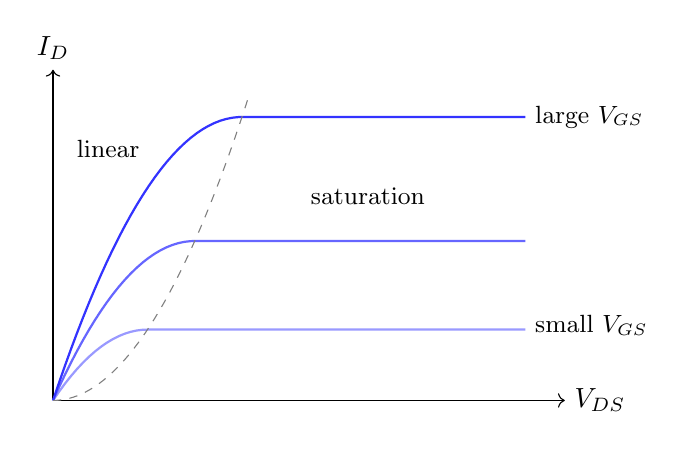
\begin{tikzpicture}[scale=1.0]
  \draw[->] (0,0) -- (6.5,0) node[right]{$V_{DS}$};
  \draw[->] (0,0) -- (0,4.2) node[above]{$I_D$};
  \foreach \v/\c in {1.2/blue!40,1.8/blue!60,2.4/blue!80} {
    \draw[thick,\c,domain=0:6,samples=80] plot (\x,{ (\x<\v) ? (\v*\x - 0.5*\x*\x)*1.25 : (0.5*\v*\v)*1.25 });
  }
  \node[right,font=\small] at (6,0.95) {small $V_{GS}$};
  \node[right,font=\small] at (6,3.6) {large $V_{GS}$};
  \draw[dashed,gray,domain=0:2.5,samples=40] plot (\x,{0.5*\x*\x*1.25});
  \node[font=\small] at (0.7,3.2) {linear};
  \node[font=\small] at (4.0,2.6) {saturation};
\end{tikzpicture}
\caption{Drain current versus drain voltage for three gate voltages. The dashed curve separates the linear region (left) from saturation (right).}
\end{figure}

What the saturation formula tells you:
\begin{itemize}
  \item \textbf{Wider is stronger}: current is proportional to $W$. Doubling the width doubles the current.
  \item \textbf{Shorter is stronger}: current is proportional to $1/L$. This is why each new manufacturing generation shrinks $L$.
  \item \textbf{More overdrive is stronger}: current grows with $(V_{GS} - \Vt)^2$. Raising the supply voltage speeds up circuits; raising the threshold slows them down.
  \item \textbf{Higher mobility is stronger}: NMOS beats PMOS of the same size.
\end{itemize}

\begin{worked}{saturation current}
An NMOS has $\mu C_{ox} = 200~\mu$A/V$^2$, $W/L = 4$, $\Vt = 0.4$\,V and $V_{GS} = 1.0$\,V, in saturation. Find $I_D$.
\[
  I_D = \tfrac12 \times 200\times10^{-6} \times 4 \times (1.0 - 0.4)^2 = 400\times10^{-6} \times 0.36 = 144~\mu\text{A}.
\]
\end{worked}

\paragraph{Real modern transistors.} The square law is a teaching model from older, longer transistors. In today's very short transistors, carriers hit their maximum velocity (velocity saturation, Chapter~\ref{ch:semis}), and current grows more like $(V_{GS} - \Vt)^{1}$ to $(V_{GS}-\Vt)^{1.3}$ than the square. Saturation current also creeps up slightly with $V_{DS}$ (\term{channel-length modulation}). The trends above still hold, and assessment questions use the simple model.

\paragraph{Subthreshold leakage.} Below threshold the current is small but not zero; it falls off \emph{exponentially} as $V_{GS}$ drops below $\Vt$, by roughly a factor of 10 for every 60 to 100\,mV at room temperature. So a transistor with a lower threshold voltage leaks exponentially more when it is ``off.'' This is the main source of leakage power (Chapter~\ref{ch:power}).

\section{Strong and weak logic levels}
\label{sec:weak1}

This section is the single most important idea for transistor-level assessment questions.

Use an NMOS as a \term{pass transistor}: its gate is held at $\VDD$ (fully on), one end is the input, and the other end drives an output node that has some capacitance (Figure~\ref{fig:passnmos}).

\begin{figure}[h]
\centering
\begin{circuitikz}
  \draw (0,0) node[nmos, rotate=-90](n){};
  \draw (n.G) -- ++(0,0.5) node[above]{gate $=\VDD$};
  \draw (n.S) -- ++(-0.8,0) node[left]{input};
  \draw (n.D) -- ++(1.0,0) coordinate(o) to[C, l=$C_{\text{load}}$] ++(0,-1.6) node[ground]{};
  \draw (o) -- ++(1.0,0) node[right]{output};
\end{circuitikz}
\caption{An NMOS pass transistor charging or discharging a load.}
\label{fig:passnmos}
\end{figure}

\paragraph{Passing a 0.} The input is 0\,V and the output starts high. The input end is the lower voltage, so it is the source, fixed at 0\,V. Then $V_{GS} = \VDD - 0 = \VDD$, comfortably above $\Vt$, for the whole discharge. The transistor stays fully on and pulls the output all the way to 0\,V. This is a \term{strong 0}.

\paragraph{Passing a 1.} The input is $\VDD$ and the output starts at 0\,V. Now the \emph{output} is the lower-voltage end, so the output is the source. As the output charges up, $V_{GS} = \VDD - V_{\text{out}}$ shrinks. When $V_{\text{out}}$ reaches $\VDD - \Vtn$, the gate is only $\Vtn$ above the source, and the transistor turns off. The output gets stuck one threshold below the supply:
\[
  V_{\text{out, max}} = \VDD - \Vtn.
\]
This is a \term{weak 1} (also called a degraded 1).

\begin{worked}{a weak 1}
$\VDD = 1.0$\,V, $\Vtn = 0.3$\,V. An NMOS pass transistor with its gate at $\VDD$ passes a 1. The output rises only to $1.0 - 0.3 = 0.7$\,V.
\end{worked}

The PMOS is the mirror image. Its source is its higher end. Passing a 1, the input (at $\VDD$) is the source, the gate is at 0, and the transistor stays fully on: a \term{strong 1}. Passing a 0, the output becomes the source; the PMOS turns off when the output falls to $|\Vtp|$, leaving a \term{weak 0}.

\begin{center}
\begin{tabular}{lll}
\toprule
 & Passes 0 & Passes 1 \\
\midrule
NMOS & strong (reaches 0\,V) & weak (stops at $\VDD - \Vtn$) \\
PMOS & weak (stops at $|\Vtp|$) & strong (reaches $\VDD$) \\
\bottomrule
\end{tabular}
\end{center}

\begin{bigidea}
NMOS is good at pulling \emph{down}; PMOS is good at pulling \emph{up}. That is why every CMOS logic gate uses NMOS transistors to connect the output to ground and PMOS transistors to connect it to the supply, and never the other way around. Chapter~\ref{ch:cmos} shows what goes wrong when you swap them.
\end{bigidea}

\paragraph{The general rule.} An NMOS whose gate is at $V_G$ can pass a voltage up to $V_G - \Vtn$, and no higher:
\[
  V_{\text{out}} = \min\left(V_{\text{in}},\; V_G - \Vtn\right).
\]
(This ignores the body effect, described below, which makes the drop slightly larger.)

\section{Chains of pass transistors}
\label{sec:passchain}

Questions often chain several pass transistors together. Two cases behave very differently.

\paragraph{Case 1: transistors in series, all gates at $\VDD$.} The threshold drop happens only \emph{once}. The first transistor passes at most $\VDD - \Vt$. The second transistor also has its gate at $\VDD$, so it too can pass up to $\VDD - \Vt$; it has no trouble passing a voltage that is already that low. The output of the chain is $\VDD - \Vt$, not $\VDD - 2\Vt$.

\paragraph{Case 2: one transistor's output drives the next transistor's gate.} Now the drops \emph{accumulate}. If node N1 is only at $\VDD - \Vt$ and it drives the gate of the next transistor, that transistor can pass only up to $(\VDD - \Vt) - \Vt$.

\begin{worked}{node voltages in a pass-transistor network}
All NMOS transistors are identical with $\Vt = 2$\,V; the supply is $\VDD = 5$\,V (an older, high-voltage process, used here to make the numbers easy to follow). Ignore the body effect.

\begin{enumerate}
  \item Transistor M1 has its gate at 5\,V and passes an input of 4\,V to node N1. \\
  $V_{N1} = \min(4,\; 5 - 2) = 3$\,V. The input is limited by the gate.
  \item Node N1 (3\,V) drives the gate of transistor M2, which passes 5\,V from the supply to node N2. \\
  $V_{N2} = \min(5,\; 3 - 2) = 1$\,V.
  \item Node N2 (1\,V) drives the gate of transistor M3. Since $1~\text{V} < \Vt = 2$\,V, M3 is off and passes nothing.
  \item Instead, suppose M1 is followed by M4, in series, also with its gate at 5\,V. The output of M4 is $\min(3,\; 5-2) = 3$\,V: no extra drop.
\end{enumerate}
\end{worked}

\begin{onoa}
A reported question asked for the voltages at several nodes of a network of identical NMOS transistors with $\VDD = 5$\,V, $\Vt = 2$\,V and an input of 4\,V. Without the original diagram, the method above is what such questions test: at each node apply $V_{\text{out}} = \min(V_{\text{in}}, V_G - \Vt)$, notice whether a gate is driven by the full supply or by an already-degraded node, and check whether any transistor's gate falls below threshold.
\end{onoa}

\section{The body effect}

So far we assumed the threshold voltage is fixed. In fact, an NMOS's threshold \emph{increases} when its source is above its body. In a pass transistor passing a 1, the source rises toward $\VDD$ while the body stays at ground, so $\Vt$ grows as the output rises, making the weak 1 even weaker. Transistors stacked in series (where the upper ones have sources above ground) are also slightly weakened. For assessment questions, it is enough to know the direction: \textbf{a source above the body raises $\Vt$}.

\section{Sizing transistors}
\label{sec:sizing}

Because current is proportional to $\mu\,W/L$, a designer chooses $W$ (and sometimes $L$) to set each transistor's strength. To make a PMOS deliver the same current as an NMOS, it must make up for its lower mobility with extra width:
\[
  \frac{(W/L)_p}{(W/L)_n} = \frac{\mu_n}{\mu_p} \approx 2 \text{ to } 3.
\]

\begin{worked}{equal saturation currents}
In a process where $\mu_n = 2.5\,\mu_p$, the NMOS in an inverter is 1\,$\mu$m wide. Both have the same length. How wide should the PMOS be so both deliver the same current?

$W_p = 2.5 \times 1 = 2.5~\mu$m.
\end{worked}

The trade-off: a wider transistor is stronger, but its gate has more capacitance, so whatever drives \emph{it} has a bigger load and becomes slower. Sizing is a balance (Chapter~\ref{ch:delay}).

\section{Transistor capacitance}

A transistor's gate is a capacitor: gate on one side, channel on the other, oxide between. Its capacitance is roughly
\[
  C_g = C_{ox}\,W\,L.
\]
The source and drain regions also have capacitance to the body, called \term{diffusion capacitance}. When a gate's output switches, it must charge the input capacitance of every gate it drives, the wires in between, and its own diffusion capacitance.

\section{Threshold voltage as a design knob}

Chip processes usually offer several transistor flavors with different thresholds:
\begin{itemize}
  \item \textbf{Low-$\Vt$} transistors: more overdrive, so faster, but they leak exponentially more when off.
  \item \textbf{High-$\Vt$} transistors: slower but with far less leakage.
\end{itemize}
Designers use fast low-$\Vt$ transistors only on the few paths that limit speed, and high-$\Vt$ transistors everywhere else to save leakage power. Temperature also changes $\Vt$: it \emph{decreases} as the chip heats up (Chapter~\ref{ch:pvt}).

\section{Modern transistor shapes}

As $L$ shrank to tens of nanometers, a gate sitting only on top of the channel could no longer fully control it, and leakage grew. Two newer structures fix this by wrapping the gate around more of the channel:
\begin{itemize}
  \item \term{FinFET}: the channel is a thin vertical fin, and the gate wraps over three sides.
  \item \term{Gate-all-around} (GAA) or \term{nanosheet}: the channel is a stack of thin horizontal sheets, each surrounded by the gate on all four sides.
\end{itemize}
More gate control means the transistor turns off more completely, which reduces leakage. The basic switch behavior in this chapter is unchanged.

\section{Summary}

\begin{itemize}
  \item A MOSFET is a voltage-controlled switch: gate controls whether current flows between source and drain. The gate draws no DC current.
  \item NMOS: on when $V_{GS} > \Vtn$ (gate high). PMOS: on when $V_{SG} > |\Vtp|$ (gate low).
  \item NMOS source is its lower-voltage end; PMOS source is its higher-voltage end.
  \item Saturation current: $I_D = \tfrac12\mu C_{ox}(W/L)(V_{GS}-\Vt)^2$. Wider, shorter, more overdrive and higher mobility all mean more current.
  \item NMOS passes a strong 0 and a weak 1 ($\VDD - \Vtn$). PMOS passes a strong 1 and a weak 0 ($|\Vtp|$).
  \item Pass-transistor rule: $V_{\text{out}} = \min(V_{\text{in}}, V_G - \Vt)$. Drops do not add in a series chain with full gates; they do add when degraded nodes drive gates.
  \item PMOS is made about 2--3 times wider than NMOS for equal current.
  \item Lower $\Vt$ means faster but exponentially leakier.
\end{itemize}

\section{Exercises}

\begin{enumerate}
  \item An NMOS has $V_{GS} = 0.2$\,V and $\Vtn = 0.35$\,V. Is it on or off?
  \item A PMOS has its source at 1.0\,V, its gate at 0\,V, and $|\Vtp| = 0.3$\,V. Is it on or off?
  \item An NMOS pass transistor with its gate at $\VDD = 1.2$\,V passes a 1. If $\Vtn = 0.4$\,V, what is the highest voltage the output reaches?
  \item A PMOS pass transistor with its gate at 0\,V passes a 0. If $|\Vtp| = 0.35$\,V, what is the lowest voltage the output reaches?
  \item An NMOS in saturation has $\mu C_{ox}(W/L) = 1$\,mA/V$^2$ and $V_{GS} - \Vt = 0.5$\,V. Find $I_D$. What happens to $I_D$ if $W$ doubles?
  \item Two NMOS transistors are in series, both gates at $\VDD = 1$\,V, $\Vt = 0.3$\,V. The input is 1\,V. What is the output: 0.7\,V or 0.4\,V?
  \item An NMOS has its gate driven by a node at 0.7\,V and passes a 1.0\,V input. With $\Vt = 0.3$\,V, what is the output?
  \item In a process with $\mu_n/\mu_p = 2$, an NMOS is 0.2\,$\mu$m wide. How wide should a same-length PMOS be for equal current?
  \item Why does a MOSFET's gate draw no DC current?
  \item What is the trade-off between low-$\Vt$ and high-$\Vt$ transistors?
\end{enumerate}

\subsection*{Answers}
\begin{enumerate}
  \item Off (below threshold), apart from a small subthreshold leakage.
  \item On: $V_{SG} = 1.0 - 0 = 1.0~\text{V} > 0.3$\,V.
  \item $1.2 - 0.4 = 0.8$\,V.
  \item $0.35$\,V.
  \item $I_D = \tfrac12 \times 1\times10^{-3} \times 0.25 = 125~\mu$A. Doubling $W$ doubles it to 250\,$\mu$A.
  \item 0.7\,V. Both gates are at the full supply, so only one threshold drop occurs.
  \item $\min(1.0,\; 0.7 - 0.3) = 0.4$\,V.
  \item 0.4\,$\mu$m.
  \item The gate is separated from the channel by an insulating oxide, so the gate is a capacitor: current flows only briefly while its voltage changes.
  \item Low-$\Vt$ is faster (more overdrive) but leaks exponentially more; high-$\Vt$ is slower but leaks far less.
\end{enumerate}

\chapter{A Short Tour of Analog Circuits}
\label{ch:analog}

Digital circuits treat voltages as just 0 or 1. Underneath, every voltage is a continuous, \term{analog} quantity, and some parts of every chip system must deal with it directly: the power supplies, the sensors, the converters between analog and digital, and the high-speed links between chips. Hardware assessments sometimes include a basic analog question, and the ideas here also deepen your understanding of transistors. This chapter is a short tour, not a full course.

\section{The transistor as an amplifier}

In Chapter~\ref{ch:mosfet} we used the transistor as a switch. Used differently, it is an \term{amplifier}: a small change in input voltage produces a large change in output voltage.

In saturation, the drain current depends on the gate voltage. A small wiggle in $V_{GS}$ produces a wiggle in $I_D$. How much current change you get per volt of gate change is the \term{transconductance}:
\[
  g_m = \frac{\Delta I_D}{\Delta V_{GS}} = \mu C_{ox}\frac{W}{L}(V_{GS}-\Vt) = \frac{2 I_D}{V_{GS}-\Vt}.
\]

\paragraph{The common-source amplifier.} Connect a resistor $R_D$ from the supply to the drain, ground the source, apply the input to the gate, and take the output from the drain (Figure~\ref{fig:csamp}). The drain voltage is $V_{\text{out}} = \VDD - I_D R_D$. A small input change $\Delta V_{\text{in}}$ changes the current by $g_m\,\Delta V_{\text{in}}$, which changes the output by $-g_m R_D\,\Delta V_{\text{in}}$. The \term{voltage gain} is
\[
  \boxed{A_v = \frac{\Delta V_{\text{out}}}{\Delta V_{\text{in}}} = -g_m R_D}
\]
The minus sign means the output moves the opposite way from the input: raising the gate pulls more current, which drops more voltage across $R_D$, which lowers the output. (A CMOS inverter is a common-source amplifier with a PMOS in place of the resistor. That is why an inverter has high gain in the middle of its range, Chapter~\ref{ch:cmos}.)

\begin{figure}[h]
\centering
\begin{circuitikz}
  \draw (0,0) node[nmos](n){};
  \draw (n.S) node[ground]{};
  \draw (n.D) to[R, l=$R_D$] ++(0,2) node[vdd]{$\VDD$};
  \draw (n.D) to[short,-o] ++(1.2,0) node[right]{$V_{\text{out}}$};
  \draw (n.G) to[short,-o] ++(-0.8,0) node[left]{$V_{\text{in}}$};
\end{circuitikz}
\caption{A common-source amplifier.}
\label{fig:csamp}
\end{figure}

\begin{worked}{amplifier gain}
An NMOS is biased at $I_D = 100~\mu$A with overdrive $V_{GS} - \Vt = 0.2$\,V, and $R_D = 10$\,k$\Omega$. Find the gain.
\[
  g_m = \frac{2 \times 100\,\mu\text{A}}{0.2\,\text{V}} = 1~\text{mA/V}, \qquad A_v = -g_m R_D = -10^{-3} \times 10^4 = -10.
\]
A 10\,mV wiggle at the input becomes a 100\,mV wiggle at the output, inverted.
\end{worked}

\section{The operational amplifier}

An \term{operational amplifier}, or op-amp, is a packaged amplifier with two inputs, $V_+$ (non-inverting) and $V_-$ (inverting), and one output. Its output is the difference between the inputs multiplied by an enormous gain $A$, often $10^5$ or more:
\[
  V_{\text{out}} = A\,(V_+ - V_-).
\]
With such huge gain, an op-amp is almost always used with \term{negative feedback}: part of the output is fed back to the $V_-$ input. Then two ``golden rules'' let you analyze circuits in seconds:

\begin{enumerate}
  \item \textbf{No current flows into the inputs.}
  \item \textbf{With negative feedback, the output adjusts itself until $V_+ = V_-$.} If they differ even slightly, the huge gain drives the output in the direction that removes the difference. (This is called a \term{virtual short}.)
\end{enumerate}

\paragraph{Inverting amplifier.} $V_+$ is grounded; the input drives $V_-$ through $R_{\text{in}}$; a feedback resistor $R_f$ connects the output back to $V_-$ (Figure~\ref{fig:opamps}, left). By rule 2, $V_- = V_+ = 0$. The current through $R_{\text{in}}$ is $V_{\text{in}}/R_{\text{in}}$; by rule 1, it all continues through $R_f$, so $V_{\text{out}} = 0 - R_f\,(V_{\text{in}}/R_{\text{in}})$:
\[
  \boxed{V_{\text{out}} = -\frac{R_f}{R_{\text{in}}}\,V_{\text{in}}}
\]

\paragraph{Non-inverting amplifier.} The input drives $V_+$ directly; $R_f$ and $R_g$ form a divider from the output to $V_-$ (Figure~\ref{fig:opamps}, right). By rule 2, $V_- = V_{\text{in}}$, and the divider gives $V_- = V_{\text{out}}\,R_g/(R_f+R_g)$:
\[
  \boxed{V_{\text{out}} = \left(1 + \frac{R_f}{R_g}\right) V_{\text{in}}}
\]

\begin{figure}[h]
\centering
\begin{circuitikz}
  \draw (0,0) node[op amp](A){};
  \draw (A.-) to[R, l_=$R_{\text{in}}$, -o] ++(-2.2,0) node[left]{$V_{\text{in}}$};
  \draw (A.+) -- ++(-0.4,0) node[ground]{};
  \draw (A.-) -- ++(0,1.3) coordinate(fb) to[R, l=$R_f$] (fb -| A.out) -- (A.out);
  \draw (A.out) to[short,-o] ++(0.8,0) node[right]{$V_{\text{out}}$};
  \node at (0,-1.6) {inverting};
\end{circuitikz}
\hspace{0.6cm}
\begin{circuitikz}
  \draw (0,0) node[op amp, noinv input up](B){};
  \draw (B.+) to[short,-o] ++(-1.2,0) node[left]{$V_{\text{in}}$};
  \draw (B.-) -- ++(-0.5,0) coordinate(m) -- ++(0,-1.0) coordinate(k);
  \draw (k) to[R, l_=$R_f$] (k -| B.out) -- (B.out);
  \draw (k) to[R, l_=$R_g$] ++(0,-1.8) node[ground]{};
  \draw (B.out) to[short,-o] ++(0.8,0) node[right]{$V_{\text{out}}$};
  \node at (0.6,-3.6) {non-inverting};
\end{circuitikz}
\caption{The two basic op-amp amplifiers.}
\label{fig:opamps}
\end{figure}

\paragraph{Voltage follower.} Connect the output straight to $V_-$ and drive $V_+$ with the input. The gain is exactly 1, so it seems useless, but it is not: the op-amp's input draws no current while its output can supply plenty. A follower lets a weak signal drive a heavy load without being dragged down. It is a \term{buffer}.

\paragraph{Comparator.} With no feedback at all, the huge gain slams the output to its maximum if $V_+ > V_-$ and to its minimum if $V_+ < V_-$. The output is effectively a digital 1 or 0 answering ``which input is bigger?'' A comparator is a one-bit analog-to-digital converter.

\section{The bipolar junction transistor, briefly}

Before MOSFETs dominated, the main transistor was the \term{bipolar junction transistor} (BJT), made of three layers: n-p-n or p-n-p. Its terminals are the \term{base}, \term{collector} and \term{emitter}. In an NPN transistor:
\begin{itemize}
  \item it turns on when the base--emitter junction is forward biased, about $V_{BE} \approx 0.7$\,V;
  \item a small base current controls a large collector current, $I_C = \beta I_B$, with $\beta$ typically around 100.
\end{itemize}
The key contrast: a MOSFET is \emph{voltage-controlled} and its gate draws no DC current; a BJT is \emph{current-controlled} and its base needs a steady current. BJTs are still used in some analog and radio circuits. For a CMOS designer they matter mostly because CMOS chips contain unwanted \emph{parasitic} BJTs that can cause latch-up (Chapter~\ref{ch:fab}).

\section{Filters}

A resistor and capacitor make a simple filter. With the capacitor to ground at the output, it is a \term{low-pass filter}: slow signals pass, fast ones are smoothed away. Swap the two components and it becomes a \term{high-pass filter}: fast changes pass, steady levels are blocked. Either way the boundary is the cutoff frequency
\[
  f_c = \frac{1}{2\pi R C}.
\]

\section{Converting between analog and digital}

An \term{analog-to-digital converter} (ADC) measures a voltage and outputs a number. An $N$-bit ADC divides its input range into $2^N$ steps. The voltage of one step, the \term{least significant bit} (LSB) or \term{resolution}, is
\[
  \boxed{\text{LSB} = \frac{V_{\text{ref}}}{2^N}}
\]
where $V_{\text{ref}}$ is the full-scale range. (Some texts divide by $2^N - 1$ instead; for large $N$ the difference is tiny. Use whichever convention a question implies.)

\begin{worked}{ADC resolution}
A 12-bit ADC has a 3.3\,V range. What voltage change corresponds to one code step?
\[
  \frac{3.3}{2^{12}} = \frac{3.3}{4096} \approx 0.806~\text{mV}.
\]
A 10-bit ADC with a 1.024\,V range has exactly $1.024/1024 = 1$\,mV per step.
\end{worked}

\paragraph{Sampling.} An ADC measures at regular intervals, the \term{sampling rate}. To capture a signal faithfully, you must sample at more than twice its highest frequency, the \term{Nyquist rate}. Sampling too slowly causes \term{aliasing}: fast signals masquerade as slow ones. Audio CDs sample at 44.1\,kHz to capture sound up to about 20\,kHz.

A \term{digital-to-analog converter} (DAC) does the reverse, turning numbers into voltages.

\section{Power supplies}

Chips need a precise, low supply voltage (around 1\,V), but power arrives at higher voltages (12\,V or more in a computer). Two kinds of circuit convert it.

\begin{itemize}
  \item A \term{linear regulator} (often an LDO, ``low-dropout'' regulator) acts like an automatically adjusted resistor in series with the load. It is simple and quiet, but it burns the voltage difference as heat. Its efficiency is about $V_{\text{out}}/V_{\text{in}}$.
  \item A \term{switching regulator} (such as a \term{buck converter}) rapidly switches the input on and off and smooths the result with an inductor and capacitor. It wastes little power, typically 85--95\% efficient. GPUs are powered by multi-phase buck converters, called voltage regulator modules (VRMs), placed close to the chip.
\end{itemize}

\begin{worked}{why linear regulators waste power}
An LDO converts 3.3\,V to 1.0\,V for a load drawing 2\,A. The same 2\,A flows through the regulator, which drops $3.3 - 1.0 = 2.3$\,V. Power wasted: $2.3 \times 2 = 4.6$\,W. Power delivered: $1.0 \times 2 = 2$\,W. Efficiency: $2/(2+4.6) \approx 30\%$, matching $V_{\text{out}}/V_{\text{in}} = 1.0/3.3$.
\end{worked}

\section{Summary}

\begin{itemize}
  \item A transistor in saturation amplifies: $g_m = 2I_D/(V_{GS}-\Vt)$; common-source gain $A_v = -g_m R_D$.
  \item Op-amp golden rules (with negative feedback): no input current; $V_+ = V_-$.
  \item Inverting gain $-R_f/R_{\text{in}}$; non-inverting gain $1 + R_f/R_g$; a follower is a unity-gain buffer; with no feedback an op-amp is a comparator.
  \item BJTs are current-controlled ($I_C = \beta I_B$, $V_{BE} \approx 0.7$\,V); MOSFETs are voltage-controlled.
  \item ADC step size $= V_{\text{ref}}/2^N$. Sample at more than twice the highest frequency.
  \item Linear regulators are simple but waste the voltage difference; switching regulators are efficient.
\end{itemize}

\section{Exercises}

\begin{enumerate}
  \item An NMOS is biased at $I_D = 200~\mu$A with overdrive 0.25\,V. Find $g_m$, and the gain of a common-source amplifier with $R_D = 5$\,k$\Omega$.
  \item An inverting amplifier has $R_{\text{in}} = 2$\,k$\Omega$ and $R_f = 10$\,k$\Omega$. If $V_{\text{in}} = 0.3$\,V, what is $V_{\text{out}}$?
  \item A non-inverting amplifier has $R_f = 9$\,k$\Omega$ and $R_g = 1$\,k$\Omega$. What is its gain?
  \item An op-amp with no feedback has $V_+ = 1.2$\,V and $V_- = 1.0$\,V. What does the output do?
  \item A 10-bit ADC has a 1.024\,V range. What is one step?
  \item A signal contains frequencies up to 20\,kHz. What is the minimum sampling rate?
  \item A linear regulator supplies 3.3\,V at 1\,A from a 5\,V input. How much power does it waste, and what is its efficiency?
\end{enumerate}

\subsection*{Answers}
\begin{enumerate}
  \item $g_m = 2 \times 200\,\mu\text{A}/0.25\,\text{V} = 1.6$\,mA/V. Gain $= -1.6\times10^{-3} \times 5000 = -8$.
  \item $V_{\text{out}} = -(10/2) \times 0.3 = -1.5$\,V.
  \item $1 + 9/1 = 10$.
  \item It swings to its maximum (positive) output, because $V_+ > V_-$. It is acting as a comparator.
  \item $1.024/1024 = 1$\,mV.
  \item More than 40\,kHz (twice 20\,kHz).
  \item Wasted: $(5 - 3.3) \times 1 = 1.7$\,W. Efficiency: $3.3/5 = 66\%$.
\end{enumerate}


\part{From Transistors to Logic}
\chapter{Binary Numbers, Bits and Boolean Algebra}
\label{ch:binary}

We now have switches (transistors). Before wiring them into logic, we need the language that logic speaks: binary numbers and Boolean algebra. This chapter covers how computers represent numbers, how to manipulate individual bits (a favorite topic of the coding part of the assessment), and the algebra used to design and simplify logic circuits.

\section{Why two values?}

A wire's voltage can take any value, so why do computers use only two, 0 and 1? Because of \emph{noise}. Every real signal picks up small unwanted disturbances: from neighboring wires, from the power supply, from temperature. If we tried to represent ten different values with ten voltage levels between 0 and 1\,V, levels would be only 0.1\,V apart, and a little noise would turn a 6 into a 7.

With only two values, we can treat \emph{any} voltage near 0 as a 0 and \emph{any} voltage near the supply as a 1, with a wide forbidden zone between. Noise has to be enormous to flip a value. Better still, each logic gate restores its output to a clean 0 or 1, so noise does not accumulate as signals pass through many gates (Chapter~\ref{ch:cmos}). Two values are the most robust choice.

One binary digit is a \term{bit}. Groups of bits have names: 4 bits are a \term{nibble}, 8 bits a \term{byte}, and a \term{word} is the natural size a processor works with (often 32 or 64 bits).

\section{Binary numbers}

In decimal, each digit position is worth ten times the one to its right: $347 = 3\times100 + 4\times10 + 7\times1$. In binary, each position is worth \emph{two} times the one to its right:
\[
  1011_2 = 1\times8 + 0\times4 + 1\times2 + 1\times1 = 11_{10}.
\]
The rightmost bit is the \term{least significant bit} (LSB); the leftmost is the \term{most significant bit} (MSB).

\paragraph{Decimal to binary.} Repeatedly divide by 2 and record the remainders; read them from last to first. For 45: $45/2 = 22$ r1, $22/2 = 11$ r0, $11/2 = 5$ r1, $5/2 = 2$ r1, $2/2 = 1$ r0, $1/2 = 0$ r1. Reading upward: $45 = 101101_2$. Check: $32+8+4+1 = 45$.

\paragraph{Powers of two to know by heart.}
\begin{center}
\begin{tabular}{ccccccc}
\toprule
$2^0$ & $2^1$ & $2^2$ & $2^3$ & $2^4$ & $2^5$ & $2^6$ \\
1 & 2 & 4 & 8 & 16 & 32 & 64 \\
\midrule
$2^7$ & $2^8$ & $2^{10}$ & $2^{12}$ & $2^{16}$ & $2^{20}$ & $2^{32}$ \\
128 & 256 & 1024 & 4096 & 65\,536 & 1\,048\,576 & $\approx 4.3\times10^9$ \\
\bottomrule
\end{tabular}
\end{center}

In computing, a ``kilobyte'' of memory usually means $2^{10} = 1024$ bytes (strictly a kibibyte, KiB), a ``megabyte'' $2^{20}$ bytes, and a ``4\,KB page'' is $2^{12} = 4096$ bytes.

\section{Hexadecimal}

Long binary strings are hard to read, so engineers write them in \term{hexadecimal} (base 16). Each hex digit stands for exactly 4 bits, using 0--9 then A--F for 10--15:

\begin{center}
\begin{tabular}{cccccccc}
\toprule
0 & 1 & 2 & 3 & 4 & 5 & 6 & 7 \\
0000 & 0001 & 0010 & 0011 & 0100 & 0101 & 0110 & 0111 \\
\midrule
8 & 9 & A & B & C & D & E & F \\
1000 & 1001 & 1010 & 1011 & 1100 & 1101 & 1110 & 1111 \\
\bottomrule
\end{tabular}
\end{center}

To convert binary to hex, split into groups of four from the right: $1011\,0111_2 = \text{B7}_{16}$. In code, hex is written with a \code{0x} prefix: \code{0xB7} $= 11\times16 + 7 = 183$. Memory addresses are almost always written in hex.

\section{How many values fit in $n$ bits?}

Each bit doubles the number of possible patterns, so $n$ bits can represent $2^n$ different values. Going the other way, to represent $N$ different things you need
\[
  n = \lceil \log_2 N \rceil \text{ bits}
\]
(the ceiling $\lceil\cdot\rceil$ means round up). For 1000 values: $2^9 = 512$ is too few, $2^{10} = 1024$ is enough, so 10 bits. This calculation appears constantly: how many flip-flops a state machine needs (Chapter~\ref{ch:fsm}), how many address bits a memory needs, how many select lines a multiplexer needs.

\section{Negative numbers: two's complement}
\label{sec:twos}

Computers almost always store signed integers in \term{two's complement}. The idea is simple: the MSB gets a \emph{negative} weight. For 8 bits, the place values are
\[
  -128,\; 64,\; 32,\; 16,\; 8,\; 4,\; 2,\; 1.
\]
So $1111\,1111_2 = -128 + 127 = -1$, and $1000\,0000_2 = -128$.

\begin{itemize}
  \item Range of $n$-bit two's complement: $-2^{n-1}$ to $2^{n-1}-1$. For 8 bits: $-128$ to $127$.
  \item The MSB tells the sign: 1 means negative.
  \item \textbf{To negate a number: invert every bit, then add 1.}
\end{itemize}

\begin{worked}{representing $-20$ in 8 bits}
$+20 = 0001\,0100$. Invert: $1110\,1011$. Add 1: $1110\,1100$. Check with weights: $-128 + 64 + 32 + 8 + 4 = -20$. Correct.
\end{worked}

The beauty of two's complement is that ordinary binary addition works for signed numbers too: the same adder hardware handles both, and subtraction is just adding the negation, $A - B = A + \nt{B} + 1$ (Chapter~\ref{ch:comb}).

\paragraph{Overflow.} If a result does not fit in $n$ bits, it wraps around. In 8 bits, $127 + 1$ gives $1000\,0000 = -128$. Signed overflow happens exactly when two numbers of the same sign are added and the result has the opposite sign.

\paragraph{Sign extension.} To widen a two's complement number, copy its sign bit into the new upper bits: $-3$ in 4 bits is $1101$; in 8 bits it is $1111\,1101$.

\section{Bitwise operations}
\label{sec:bitops}

Programming languages (and hardware) can operate on every bit of a word at once:

\begin{center}
\begin{tabular}{llll}
\toprule
Operation & C syntax & Rule per bit & Example (\code{1100} op \code{1010}) \\
\midrule
AND & \code{a \& b} & 1 only if both are 1 & \code{1000} \\
OR & \code{a | b} & 1 if either is 1 & \code{1110} \\
XOR & \code{a \^{} b} & 1 if they differ & \code{0110} \\
NOT & \code{\~{}a} & flip every bit & \code{\~{}1100 = 0011} \\
Left shift & \code{a << k} & move bits left, fill with 0 & \code{0011 << 1 = 0110} \\
Right shift & \code{a >> k} & move bits right & \code{1100 >> 2 = 0011} \\
\bottomrule
\end{tabular}
\end{center}

Shifting left by $k$ multiplies by $2^k$; shifting right by $k$ divides by $2^k$ (rounding down) for unsigned numbers. So with \code{i = 8} and \code{j = 2}, \code{i << j} is 32 and \code{i >> j} is 2. For \emph{signed} numbers, a right shift usually copies the sign bit in from the left (an \term{arithmetic shift}) so negative numbers stay negative; unsigned values get zeros (a \term{logical shift}).

\subsection*{Bit tricks worth knowing}

Using a \term{mask} (a word with 1s only where you care), you can work on individual bits:

\begin{center}
\begin{tabular}{ll}
\toprule
Goal & Expression \\
\midrule
Read bit $k$ & \code{(x >> k) \& 1} \\
Set bit $k$ to 1 & \code{x | (1 << k)} \\
Clear bit $k$ to 0 & \code{x \& \~{}(1 << k)} \\
Toggle bit $k$ & \code{x \^{} (1 << k)} \\
Keep only the lowest set bit & \code{x \& (-x)} \\
Clear the lowest set bit & \code{x \& (x - 1)} \\
Is $x$ a power of two? & \code{x != 0 \&\& (x \& (x - 1)) == 0} \\
Mask of bits \code{lo} to \code{hi} & \code{((1 << (hi - lo + 1)) - 1) << lo} \\
\bottomrule
\end{tabular}
\end{center}

Why does \code{x \& (x-1)} clear the lowest set bit? Subtracting 1 flips the lowest 1 to 0 and all the 0s below it to 1s, and leaves everything above unchanged. ANDing with the original keeps the upper bits and zeros the rest. A power of two has exactly one 1 bit, so clearing it leaves zero.

\begin{worked}{building a bit mask}
Build a mask with 1s in bits 4 through 7. Width $= 7 - 4 + 1 = 4$. \code{(1 << 4) - 1} $= 1111_2$. Shift left by 4: $1111\,0000_2 =$ \code{0xF0}. (Careful: if the width is the full 32 bits, \code{1 << 32} overflows a 32-bit integer in C; use a 64-bit type for the intermediate value.)
\end{worked}

\begin{worked}{are two addresses on the same 4\,KB page?}
Memory is divided into pages of $4096 = 2^{12}$ bytes. The low 12 bits of an address are the offset within a page; the remaining upper bits are the \emph{page number}. Two addresses are on the same page exactly when their page numbers match:
\begin{center}
\code{(a >> 12) == (b >> 12)} \qquad or equivalently \qquad \code{((a \^{} b) \& \~{}0xFFF) == 0}
\end{center}
\code{0x12345FF0} and \code{0x12345010}: both have page number \code{0x12345}, so same page. \code{0x12345FFF} and \code{0x12346000}: page numbers \code{0x12345} and \code{0x12346}, so different pages, even though the addresses differ by only 1.
\end{worked}

\begin{onoa}
Both of the worked examples above match coding problems reported on NVIDIA's Ignite assessment: building a bit mask from bit \code{lo} to bit \code{hi}, and checking whether two 32-bit addresses fall on the same 4\,KB page. Chapter~\ref{ch:prog} has full code.
\end{onoa}

\subsection*{XOR, the most useful operator}

XOR has algebraic properties that make it a favorite in puzzles and in hardware:
\begin{itemize}
  \item $a \oplus 0 = a$ and $a \oplus a = 0$: XORing with a value twice cancels it.
  \item $a \oplus 1 = \nt{a}$: XOR with 1 inverts. So XOR is a \emph{controlled inverter}.
  \item XOR is commutative and associative, so order does not matter.
  \item The XOR of all bits of a word is its \term{parity}: 1 if it has an odd number of 1s.
\end{itemize}
A consequence used in coding problems: if $P_i$ is the XOR of the first $i$ elements of an array (a \term{prefix XOR}), then the XOR of elements $l$ through $r$ is $P_{r+1} \oplus P_l$, because everything before $l$ appears twice and cancels.

\section{Gray code}
\label{sec:gray}

In ordinary binary, counting from 3 ($011$) to 4 ($100$) changes three bits at once. If those bits are read at the wrong moment, while some have changed and some have not, you can get any value at all. \term{Gray code} orders the numbers so that \emph{exactly one bit changes} between neighbors:

\begin{center}
\begin{tabular}{lcccccccc}
\toprule
Decimal & 0 & 1 & 2 & 3 & 4 & 5 & 6 & 7 \\
Binary & 000 & 001 & 010 & 011 & 100 & 101 & 110 & 111 \\
Gray & 000 & 001 & 011 & 010 & 110 & 111 & 101 & 100 \\
\bottomrule
\end{tabular}
\end{center}

Conversion: $g = b \oplus (b \gg 1)$. Gray code is used for counters that are read by a different clock (Chapter~\ref{ch:rtl}) and to label Karnaugh maps (below).

\section{Boolean algebra}

\term{Boolean algebra}, named after George Boole, is the mathematics of variables that are only 0 or 1. It has three basic operations:
\begin{itemize}
  \item AND, written $A \cdot B$ or just $AB$: 1 only if both are 1.
  \item OR, written $A + B$: 1 if at least one is 1. (Here $1 + 1 = 1$.)
  \item NOT, written $\nt{A}$ (or $A'$): the opposite value.
\end{itemize}
Precedence, as in ordinary algebra: NOT first, then AND, then OR. So $A + BC$ means $A + (B \cdot C)$.

Combined truth table of the common two-input functions:
\begin{center}
\begin{tabular}{cc|ccccccc}
\toprule
$A$ & $B$ & AND & OR & NAND & NOR & XOR & XNOR \\
\midrule
0 & 0 & 0 & 0 & 1 & 1 & 0 & 1 \\
0 & 1 & 0 & 1 & 1 & 0 & 1 & 0 \\
1 & 0 & 0 & 1 & 1 & 0 & 1 & 0 \\
1 & 1 & 1 & 1 & 0 & 0 & 0 & 1 \\
\bottomrule
\end{tabular}
\end{center}

\subsection*{The laws}

\begin{center}
\begin{tabular}{lll}
\toprule
Law & OR form & AND form \\
\midrule
Identity & $A + 0 = A$ & $A \cdot 1 = A$ \\
Null & $A + 1 = 1$ & $A \cdot 0 = 0$ \\
Idempotent & $A + A = A$ & $A \cdot A = A$ \\
Complement & $A + \nt{A} = 1$ & $A \cdot \nt{A} = 0$ \\
Involution & \multicolumn{2}{l}{$\nt{\nt{A}} = A$} \\
Commutative & $A + B = B + A$ & $AB = BA$ \\
Associative & $(A+B)+C = A+(B+C)$ & $(AB)C = A(BC)$ \\
Distributive & $A + BC = (A+B)(A+C)$ & $A(B+C) = AB + AC$ \\
Absorption & $A + AB = A$ & $A(A+B) = A$ \\
Also useful & $A + \nt{A}B = A + B$ & $A(\nt{A} + B) = AB$ \\
De Morgan & $\nt{A + B} = \nt{A}\,\nt{B}$ & $\nt{AB} = \nt{A} + \nt{B}$ \\
Consensus & \multicolumn{2}{l}{$AB + \nt{A}C + BC = AB + \nt{A}C$} \\
\bottomrule
\end{tabular}
\end{center}

Two of these surprise people because they do not hold in ordinary algebra: $A + 1 = 1$, and the first distributive law $A + BC = (A+B)(A+C)$. Check any law yourself with a truth table; that is always a valid proof.

\begin{bigidea}
\textbf{De Morgan's laws}: to complement an expression, swap AND with OR and complement each variable. ``Not (A or B)'' is ``not A and not B.'' These laws are why a NAND gate is the same as an OR gate with inverted inputs, and they are the key to building logic from transistors (Chapter~\ref{ch:cmos}).
\end{bigidea}

\begin{worked}{simplifying}
Simplify $F = AB + A\nt{B} + \nt{A}B$.

$AB + A\nt{B} = A(B + \nt{B}) = A$. So $F = A + \nt{A}B = A + B$.
\end{worked}

\section{From a truth table to an expression}

Any truth table can be turned into a formula:

\begin{itemize}
  \item \textbf{Sum of products (SOP)}: for each row where the output is 1, write an AND term (a \term{minterm}) that is 1 only for that row, then OR them all. For $A=0, B=1$, the minterm is $\nt{A}B$.
  \item \textbf{Product of sums (POS)}: for each row where the output is 0, write an OR term (a \term{maxterm}) that is 0 only for that row, then AND them.
\end{itemize}

Minterms are numbered by the row's binary value; $F = \sum m(1,2)$ means ``1 in rows 1 and 2.'' For two inputs, that is $\nt{A}B + A\nt{B} = A \oplus B$.

\paragraph{How many functions are there?} An $n$-input truth table has $2^n$ rows, and each row's output can be 0 or 1 independently, so there are $2^{2^n}$ different functions. For 2 inputs: $2^4 = 16$. For 3 inputs: $2^8 = 256$.

\section{Karnaugh maps}

A \term{Karnaugh map} (K-map) is a truth table drawn as a grid so that simplifications become visible. Rows and columns are labeled in Gray code, so any two neighboring cells differ in exactly one variable. When two neighboring cells are both 1, that variable does not matter, and the two minterms merge into one simpler term.

Rules for grouping the 1s:
\begin{enumerate}
  \item Groups are rectangles of 1, 2, 4, 8 or 16 cells (powers of two).
  \item Groups may wrap around the edges: the left column neighbors the right column, and the top row neighbors the bottom row (the four corners are neighbors too).
  \item Make each group as large as possible, and use as few groups as possible. Groups may overlap.
  \item Each group becomes one product term containing only the variables that stay constant across the group.
  \item ``Don't care'' cells (inputs that never occur, written $X$) may be included in groups if that helps, or ignored.
\end{enumerate}

\begin{figure}[h]
\centering
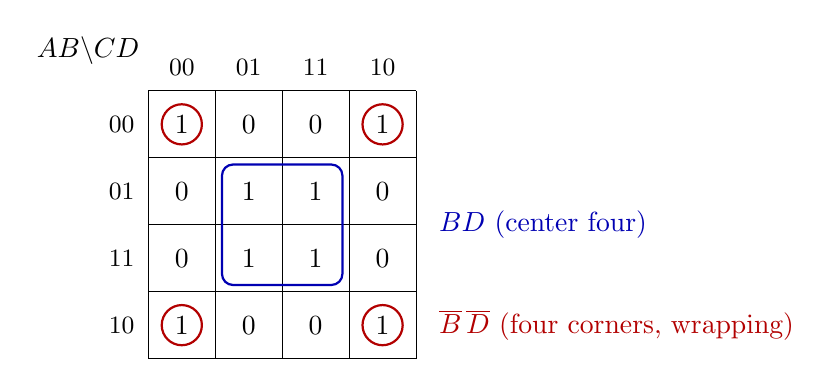
\begin{tikzpicture}[scale=0.85]
  \foreach \i in {0,...,4} { \draw (\i,0) -- (\i,4); \draw (0,\i) -- (4,\i); }
  \node at (-0.9,4.6) {$AB \backslash CD$};
  \foreach \lab [count=\c from 0] in {00,01,11,10} {
    \node at (\c+0.5,4.35) {\small \lab};
    \node at (-0.4,3.5-\c) {\small \lab};}
  % rows: 00: 1 0 0 1 ; 01: 0 1 1 0 ; 11: 0 1 1 0 ; 10: 1 0 0 1
  \foreach \c/\r/\v in {0/0/1,1/0/0,2/0/0,3/0/1, 0/1/0,1/1/1,2/1/1,3/1/0,
                       0/2/0,1/2/1,2/2/1,3/2/0, 0/3/1,1/3/0,2/3/0,3/3/1}
    \node at (\c+0.5,3.5-\r) {\v};
  \draw[blue!70!black,thick,rounded corners] (1.1,1.1) rectangle (2.9,2.9);
  \node[blue!70!black,right] at (4.2,2) {$BD$ (center four)};
  \foreach \c/\r in {0/0,3/0,0/3,3/3}
    \draw[red!70!black,thick] (\c+0.5,3.5-\r) circle (0.3);
  \node[red!70!black,right] at (4.2,0.5) {$\nt{B}\,\nt{D}$ (four corners, wrapping)};
\end{tikzpicture}
\caption{K-map for $F = \sum m(0,2,5,7,8,10,13,15)$. Two groups of four give $F = BD + \nt{B}\,\nt{D}$.}
\label{fig:kmap}
\end{figure}

\begin{worked}{a four-variable K-map}
Simplify $F(A,B,C,D) = \sum m(0,2,5,7,8,10,13,15)$ (Figure~\ref{fig:kmap}).

The center four cells have $B=1$ and $D=1$ while $A$ and $C$ vary: the group is $BD$. The four corner cells are neighbors through wrap-around; they have $B = 0$ and $D = 0$: the group is $\nt{B}\,\nt{D}$. So $F = BD + \nt{B}\,\nt{D}$, which is $B \text{ XNOR } D$. Eight minterms collapsed into one two-input gate.
\end{worked}

\section{Summary}

\begin{itemize}
  \item Binary uses two values because they are the most robust against noise.
  \item $n$ bits hold $2^n$ values; $N$ values need $\lceil\log_2 N\rceil$ bits. Hex digits are 4 bits each.
  \item Two's complement: MSB has weight $-2^{n-1}$; negate by inverting and adding 1; range $-2^{n-1}$ to $2^{n-1}-1$.
  \item Shifts multiply and divide by powers of two; masks select bits; \code{x \& (x-1)} clears the lowest set bit.
  \item Same 4\,KB page: compare \code{a >> 12} with \code{b >> 12}.
  \item XOR: $a \oplus a = 0$, $a \oplus 1 = \nt{a}$; prefix XOR gives any subarray's XOR.
  \item Gray code changes one bit at a time.
  \item Boolean laws, especially De Morgan; SOP from the 1-rows; K-maps group neighboring 1s in powers of two.
\end{itemize}

\section{Exercises}

\begin{enumerate}
  \item Convert 45 to binary and to hex.
  \item Convert \code{0xB7} to decimal and to binary.
  \item What is the range of an 8-bit two's complement number? Write $-20$ and $-1$ in 8-bit two's complement.
  \item How many bits are needed to give 1000 items unique IDs?
  \item For \code{x = 0b10110110}, compute \code{x \& (x - 1)} and \code{x \& (-x)}.
  \item Are \code{0x7FFFF000} and \code{0x7FFFFFFF} on the same 4\,KB page? What about \code{0x00001FFF} and \code{0x00002000}?
  \item Write a mask with 1s in bits 8 through 11 (bit 0 is the LSB), in hex.
  \item Simplify: (a) $A + \nt{A}B$; (b) $(A+B)(A+C)$; (c) apply De Morgan to $\nt{AB + C}$.
  \item Use a K-map (or algebra) to simplify $F(A,B,C) = \sum m(1,3,5,7)$.
  \item How many different Boolean functions of 3 inputs exist?
  \item What is the 3-bit Gray code for the number 6?
  \item In C, with \code{int i = 8, j = 2;}, what do \code{i << j} and \code{i >> j} evaluate to?
\end{enumerate}

\subsection*{Answers}
\begin{enumerate}
  \item $45 = 101101_2 = \code{0x2D}$.
  \item $\code{0xB7} = 183 = 1011\,0111_2$.
  \item $-128$ to $127$. $-20 = 1110\,1100$. $-1 = 1111\,1111$.
  \item 10 bits ($2^{10} = 1024 \ge 1000$).
  \item \code{x \& (x-1)} $= 1011\,0100$ (lowest set bit, bit 1, cleared). \code{x \& (-x)} $= 0000\,0010$ (only the lowest set bit kept).
  \item First pair: both have page number \code{0x7FFFF}, so yes. Second pair: \code{0x00001} versus \code{0x00002}, so no.
  \item \code{0xF00}.
  \item (a) $A + B$. (b) $A + BC$. (c) $\nt{AB}\cdot\nt{C} = (\nt{A} + \nt{B})\,\nt{C}$.
  \item The 1s are exactly the rows where $C = 1$, so $F = C$.
  \item $2^{2^3} = 256$.
  \item $6 = 110_2$; $g = 110 \oplus 011 = 101$.
  \item 32 and 2.
\end{enumerate}

\chapter{Building Logic Gates from Transistors}
\label{ch:cmos}

We have switches (Chapter~\ref{ch:mosfet}) and the algebra of 0s and 1s (Chapter~\ref{ch:binary}). This chapter joins them: it shows how NMOS and PMOS transistors are wired into logic gates, why the standard arrangement works so well, and what goes wrong when it is changed, including the swapped-inverter question from the assessment.

\section{The rule of complementary logic}

Every standard logic gate in a modern chip uses \term{static CMOS} (complementary MOS) design. Its output node is connected to two networks of transistors:

\begin{itemize}
  \item a \term{pull-up network} (PUN) of PMOS transistors, between the supply $\VDD$ and the output, which connects the output to 1;
  \item a \term{pull-down network} (PDN) of NMOS transistors, between the output and ground, which connects the output to 0.
\end{itemize}

The two networks are designed so that, for every combination of inputs, \emph{exactly one} of them conducts. The output is therefore always firmly connected to either the supply or ground, never to both and never to neither.

Why PMOS on top and NMOS on the bottom? Because of the strong and weak levels from Section~\ref{sec:weak1}: PMOS passes a strong 1 and NMOS passes a strong 0. Each transistor is placed where it is good.

\section{The CMOS inverter}

The simplest gate is the \term{inverter} (NOT gate): one PMOS and one NMOS, gates tied together as the input, drains tied together as the output (Figure~\ref{fig:inverter}).

\begin{figure}[h]
\centering
\begin{circuitikz}
  \draw (0,0) node[pmos](p){} (0,-2.2) node[nmos](n){};
  \draw (p.S) node[vdd]{$\VDD$};
  \draw (n.S) node[ground]{};
  \draw (p.D) -- (n.D);
  \draw (p.G) -- (n.G);
  \draw ($(p.G)!0.5!(n.G)$) to[short,-o] ++(-1,0) node[left]{In};
  \draw ($(p.D)!0.5!(n.D)$) to[short,*-o] ++(1.3,0) node[right]{Out};
\end{circuitikz}
\hspace{1.5cm}
\begin{circuitikz}
  \draw (0,0) node[not port](i){};
  \draw (i.in) -- ++(-0.4,0) node[left]{In};
  \draw (i.out) -- ++(0.4,0) node[right]{Out};
  \node at (0,-1.2) {logic symbol};
\end{circuitikz}
\caption{The CMOS inverter and its logic symbol.}
\label{fig:inverter}
\end{figure}

\begin{itemize}
  \item \textbf{Input = 0:} the PMOS is on (gate low) and the NMOS is off. The output connects to $\VDD$: output = 1.
  \item \textbf{Input = 1:} the NMOS is on and the PMOS is off. The output connects to ground: output = 0.
\end{itemize}

Three properties make this the ideal gate:
\begin{enumerate}
  \item \textbf{Full swing.} The output reaches exactly $\VDD$ and exactly 0\,V, because each transistor passes its strong level.
  \item \textbf{No static current.} In either steady state one transistor is off, so there is no path from supply to ground. An idle inverter burns only tiny leakage power.
  \item \textbf{Restoring.} The output is driven by the supply rails, not by the input, so a slightly noisy input still produces a clean output.
\end{enumerate}

\section{The voltage transfer characteristic}

What happens for inputs between 0 and $\VDD$? Plotting the output voltage against the input voltage gives the \term{voltage transfer characteristic} (VTC), Figure~\ref{fig:vtc}.

\begin{figure}[h]
\centering
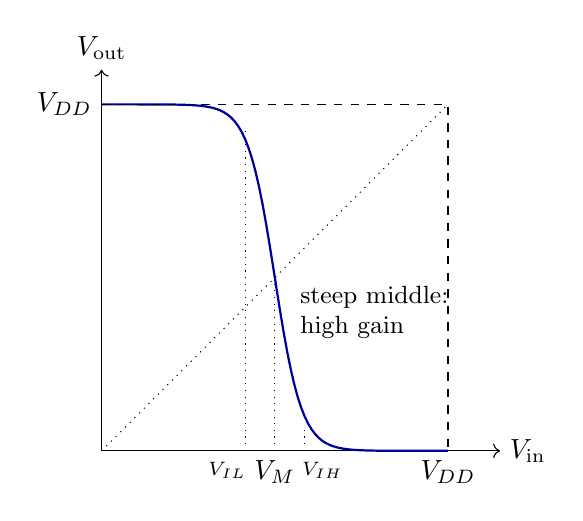
\begin{tikzpicture}[scale=1.1]
  \draw[->] (0,0) -- (4.6,0) node[right]{$V_{\text{in}}$};
  \draw[->] (0,0) -- (0,4.4) node[above]{$V_{\text{out}}$};
  \draw[thick,blue!60!black,domain=0:4,samples=100] plot (\x,{2*(1-tanh(3.2*(\x-2)))});
  \draw[dashed] (0,4) node[left]{$\VDD$} -- (4,4) -- (4,0) node[below]{$\VDD$};
  \draw[dotted] (0,0) -- (4,4);
  \draw[dotted] (2,0) node[below]{$V_M$} -- (2,2);
  \draw[dotted] (1.66,0) -- (1.66,3.75); \node[below] at (1.45,-0.02) {\scriptsize $V_{IL}$};
  \draw[dotted] (2.34,0) -- (2.34,0.25); \node[below] at (2.55,-0.02) {\scriptsize $V_{IH}$};
  \node[font=\small,align=left] at (3.15,1.6) {steep middle:\\high gain};
\end{tikzpicture}
\caption{Voltage transfer characteristic of an inverter. Where the curve crosses the diagonal, $V_{\text{in}} = V_{\text{out}} = V_M$.}
\label{fig:vtc}
\end{figure}

\begin{itemize}
  \item For low inputs the output stays near $\VDD$; for high inputs it stays near 0. In between, it drops steeply.
  \item In the steep middle both transistors are partly on. A current flows straight from supply to ground for the short time the input spends there (the short-circuit current, Chapter~\ref{ch:power}).
  \item The \term{switching threshold} $V_M$ is the input voltage at which $V_{\text{out}} = V_{\text{in}}$. With equally strong pull-up and pull-down (PMOS sized up to match the NMOS), $V_M = \VDD/2$. A stronger PMOS shifts $V_M$ higher, a stronger NMOS shifts it lower: the stronger side wins the tug-of-war, just like a voltage divider (Chapter~\ref{ch:electricity}).
  \item The steep middle means \emph{high gain}: the inverter acts as an amplifier there (Chapter~\ref{ch:analog}). This gain is what lets gates clean up noisy signals.
\end{itemize}

\paragraph{Noise margins.} Define four voltages:
\begin{itemize}
  \item $V_{OH}$, $V_{OL}$: the output levels a gate actually produces for 1 and 0;
  \item $V_{IH}$: the lowest input voltage guaranteed to be read as 1;
  \item $V_{IL}$: the highest input voltage guaranteed to be read as 0.
\end{itemize}
($V_{IL}$ and $V_{IH}$ are usually taken where the VTC's slope is $-1$.) The \term{noise margins} are how much noise a signal can pick up between one gate and the next and still be read correctly:
\[
  NM_H = V_{OH} - V_{IH}, \qquad NM_L = V_{IL} - V_{OL}.
\]
Larger is better. A CMOS inverter has $V_{OH} = \VDD$ and $V_{OL} = 0$, which gives it large noise margins.

\section{The swapped inverter}
\label{sec:swapped}

Now the assessment question. Take an inverter and swap the transistors: the NMOS now connects the output to $\VDD$, and the PMOS connects the output to ground (Figure~\ref{fig:swapped}). What does the circuit do?

\begin{figure}[h]
\centering
\begin{circuitikz}
  \draw (0,0) node[nmos](n){} (0,-2.4) node[pmos, xscale=1](p){};
  \draw (n.D) node[vdd]{$\VDD$};
  \draw (p.D) node[ground]{};
  \draw (n.S) -- (p.S);
  \draw (n.G) -- (p.G);
  \draw ($(n.G)!0.5!(p.G)$) to[short,-o] ++(-1,0) node[left]{In};
  \draw ($(n.S)!0.5!(p.S)$) to[short,*-o] ++(1.3,0) node[right]{Out};
  \node[right,font=\small] at (0.6,0.3) {NMOS on top};
  \node[right,font=\small] at (0.6,-2.7) {PMOS on bottom};
\end{circuitikz}
\caption{The ``swapped'' inverter: NMOS to the supply, PMOS to ground.}
\label{fig:swapped}
\end{figure}

Work through both inputs using the rules from Chapter~\ref{ch:mosfet}. Let $\VDD = 1.0$\,V, $\Vtn = 0.3$\,V and $|\Vtp| = 0.3$\,V.

\paragraph{Input = 1 ($\VDD$).} The top NMOS has its gate high, so it turns on and starts pulling the output \emph{up} toward $\VDD$. The bottom PMOS has its gate high, so it is off. But the NMOS is passing a 1, and NMOS passes a weak 1: the output is the NMOS's source, and the transistor turns off when the output reaches $\VDD - \Vtn = 0.7$\,V. The output settles at about 0.7\,V.

\paragraph{Input = 0.} The top NMOS is off. The bottom PMOS has its gate at 0, so it turns on and pulls the output \emph{down}. But PMOS passes a weak 0: the output is the PMOS's source, and the transistor turns off when the output falls to $|\Vtp| = 0.3$\,V. The output settles at about 0.3\,V.

\begin{center}
\begin{tabular}{ccc}
\toprule
Input & Normal inverter output & Swapped circuit output \\
\midrule
0 & $\VDD$ (strong 1) & $|\Vtp| = 0.3$\,V (weak 0) \\
1 & 0 (strong 0) & $\VDD - \Vtn = 0.7$\,V (weak 1) \\
\bottomrule
\end{tabular}
\end{center}

\begin{onoa}
The swapped circuit \textbf{no longer inverts}. It is a \textbf{non-inverting buffer with degraded output levels}: a high input gives a weak high ($\VDD - \Vtn$), and a low input gives a weak low ($|\Vtp|$). Each transistor acts as a \emph{source follower}: its output follows its gate, one threshold behind. The output swing is reduced, drive strength is weak (the transistors turn off as the output approaches its final value, so it gets there slowly), noise margins shrink, and the gain is less than 1, so the circuit cannot clean up noise. Chaining such stages makes it worse: in the simple model, a second stage driven by 0.7\,V can only reach $0.7 - 0.3 = 0.4$\,V, and the logic levels collapse.
\end{onoa}

The lesson generalizes: whenever a question puts NMOS in a pull-up position or PMOS in a pull-down position, expect a threshold-voltage drop on that level.

\section{NAND and NOR gates}

\subsection*{The two-input NAND}

A NAND gate's output is 0 only when both inputs are 1. So the pull-down network must conduct only when $A = 1$ \emph{and} $B = 1$: two NMOS transistors \textbf{in series} (current must pass through both, so both must be on). The pull-up must conduct whenever $A = 0$ \emph{or} $B = 0$: two PMOS transistors \textbf{in parallel} (either one can connect the output to $\VDD$). See Figure~\ref{fig:nandnor}, left.

\subsection*{The two-input NOR}

A NOR gate's output is 0 when $A = 1$ \emph{or} $B = 1$: two NMOS \textbf{in parallel}. Its output is 1 only when both inputs are 0: two PMOS \textbf{in series} (Figure~\ref{fig:nandnor}, right).

\begin{figure}[h]
\centering
\begin{circuitikz}[scale=0.9, transform shape]
  % NAND2
  \draw (0,0) node[pmos](pa){} (2,0) node[pmos](pb){};
  \draw (pa.S) -- (pb.S); \draw ($(pa.S)!0.5!(pb.S)$) node[vdd]{$\VDD$};
  \draw (pa.D) -- (pb.D);
  \draw (pb.D) -- ++(0,-0.6) coordinate(out);
  \draw (out) to[short,*-o] ++(1.2,0) node[right]{Out};
  \draw (out) -- ++(0,-0.3) coordinate(t);
  \draw (t) ++(0,-0.77) node[nmos,anchor=D](na){};
  \draw (na.S) ++(0,-0.77) node[nmos,anchor=D](nb){};
  \draw (t) -- (na.D);
  \draw (na.S) -- (nb.D);
  \draw (nb.S) node[ground]{};
  \node[left] at (pa.G) {A}; \node[left] at (pb.G) {B};
  \node[left] at (na.G) {A}; \node[left] at (nb.G) {B};
  \node at (1,-7.5) {NAND: PMOS parallel, NMOS series};
\end{circuitikz}
\hspace{1cm}
\begin{circuitikz}[scale=0.9, transform shape]
  % NOR2
  \draw (0,0) node[pmos](pa){};
  \draw (pa.S) node[vdd]{$\VDD$};
  \draw (pa.D) ++(0,-0.77) node[pmos,anchor=S](pb){};
  \draw (pa.D) -- (pb.S);
  \draw (pb.D) -- ++(0,-0.5) coordinate(out);
  \draw (out) to[short,*-o] ++(2.6,0) node[right]{Out};
  \draw (out) ++(0,-0.3) coordinate(t);
  \draw (out) -- (t);
  \draw (t) -- ++(2.0,0) coordinate(t2);
  \draw (t) ++(0,-0.77) node[nmos,anchor=D](na){};
  \draw (t2) ++(0,-0.77) node[nmos,anchor=D](nb){};
  \draw (t) -- (na.D); \draw (t2) -- (nb.D);
  \draw (na.S) -- (nb.S);
  \draw ($(na.S)!0.5!(nb.S)$) node[ground]{};
  \node[left] at (pa.G) {A}; \node[left] at (pb.G) {B};
  \node[left] at (na.G) {A}; \node[left] at (nb.G) {B};
  \node at (1.0,-7.5) {NOR: PMOS series, NMOS parallel};
\end{circuitikz}
\caption{Two-input NAND (left) and NOR (right). In each, the pull-up network is the \emph{dual} of the pull-down: series becomes parallel and parallel becomes series.}
\label{fig:nandnor}
\end{figure}

\begin{bigidea}
In the pull-down network, \textbf{series NMOS means AND} (all must be on) and \textbf{parallel NMOS means OR} (any can be on). The pull-up network is the \textbf{dual}: swap series and parallel, and use PMOS. This guarantees exactly one network conducts for every input combination.
\end{bigidea}

\section{Designing any gate}

The same recipe builds any inverting function:
\begin{enumerate}
  \item Write the function as $F = \nt{\text{something}}$, where ``something'' uses only ANDs and ORs of the inputs. That ``something'' is when the output should be 0.
  \item Build the pull-down network from it: AND becomes series NMOS, OR becomes parallel NMOS.
  \item Build the pull-up network as the dual: swap series and parallel, use PMOS, same inputs.
\end{enumerate}

\begin{worked}{an AND-OR-INVERT gate}
Build $F = \nt{AB + C}$ (called AOI21: AND-OR-INVERT with a 2-input AND and a 1-input term).

Pull-down conducts when $AB + C = 1$: NMOS $A$ in series with NMOS $B$, and that pair in parallel with NMOS $C$.

Pull-up is the dual: PMOS $A$ in parallel with PMOS $B$, and that pair in series with PMOS $C$.

Total: 6 transistors. Building the same function from separate AND, OR and NOT gates would take 12 or more, and be slower. Compound gates like AOI and OAI (OR-AND-INVERT) are common for this reason.
\end{worked}

\paragraph{Why static CMOS gates always invert.} In a single stage, turning an input \emph{on} (to 1) can only turn NMOS transistors on, which can only pull the output \emph{down}. So a rising input can only cause a falling output. A non-inverting function needs two stages: AND is a NAND followed by an inverter, OR is a NOR followed by an inverter.

\begin{center}
\begin{tabular}{lc}
\toprule
Gate & Transistors (static CMOS) \\
\midrule
Inverter & 2 \\
NAND2, NOR2 & 4 \\
NAND3, NOR3 & 6 \\
AND2, OR2 (gate + inverter) & 6 \\
AOI21, OAI21 & 6 \\
XOR2 (straightforward static design) & 12 \\
\bottomrule
\end{tabular}
\end{center}
An $n$-input static CMOS gate uses $2n$ transistors: one NMOS and one PMOS per input.

\section{Why NAND is preferred over NOR}

NAND and NOR are both universal (Chapter~\ref{ch:comb}), but designers strongly prefer NAND. The reason is mobility. Transistors in series are slower, because their resistances add (Chapter~\ref{ch:electricity}). A NAND puts its series stack in the NMOS, which is the fast device. A NOR puts its series stack in the PMOS, which is already about two to three times slower. To compensate, the series PMOS in a NOR must be made very wide, which costs area and adds input capacitance.

Sizing for the same strength as a reference inverter (NMOS width 1, PMOS width 2, assuming $\mu_n = 2\mu_p$):
\begin{center}
\begin{tabular}{lll}
\toprule
Gate & Each NMOS & Each PMOS \\
\midrule
Inverter & 1 & 2 \\
NAND2 & 2 (two in series) & 2 (in parallel) \\
NOR2 & 1 (in parallel) & 4 (two in series) \\
\bottomrule
\end{tabular}
\end{center}
Two transistors in series act like one with twice the resistance, so each must be twice as wide to keep the same total strength. The NOR's PMOS pair ends up four times the NMOS width.

\paragraph{Fan-in limits.} The more inputs a gate has, the taller its series stack. Tall stacks are slow, both because resistances add and because the upper transistors suffer the body effect (Chapter~\ref{ch:mosfet}). Gates are usually limited to about four inputs; wider functions are built as trees of smaller gates.

\section{Pass transistors and transmission gates}

Instead of connecting outputs to the supply rails, a \term{pass transistor} simply passes an input signal through. A single NMOS pass transistor is small, but it passes a weak 1. The fix is the \term{transmission gate} (TG): an NMOS and a PMOS in parallel, controlled by opposite signals (Figure~\ref{fig:tg}). When the control is on, both conduct: the NMOS carries the 0s well and the PMOS carries the 1s well, so the TG passes \emph{both} levels at full strength.

\begin{figure}[h]
\centering
\begin{circuitikz}
  \draw (0,0) node[nmos, rotate=90](n){};
  \draw (0,1.8) node[pmos, rotate=-90](p){};
  \draw (n.D) -- (p.D); \draw (n.S) -- (p.S);
  \draw ($(n.D)!0.5!(p.D)$) to[short,*-o] ++(-1,0) node[left]{In};
  \draw ($(n.S)!0.5!(p.S)$) to[short,*-o] ++(1,0) node[right]{Out};
  \draw (n.G) -- ++(0,-0.4) node[below]{$S$};
  \draw (p.G) -- ++(0,0.4) node[above]{$\nt{S}$};
\end{circuitikz}
\caption{A transmission gate: when $S = 1$, both transistors conduct and the input passes to the output at full strength.}
\label{fig:tg}
\end{figure}

Transmission gates make compact multiplexers (two TGs and an inverter make a 2:1 mux), XOR gates, and the latches inside flip-flops (Chapter~\ref{ch:latch}). Their drawback is that they do not restore signal levels or add drive; a long chain of TGs gets slow and must be broken up with buffers.

\section{Tristate buffers}

Sometimes several circuits must share one wire, such as a bus. Only one may drive it at a time; the others must disconnect. A \term{tristate buffer} has an enable input. When enabled, it drives its input value (0 or 1) onto the output. When disabled, both its pull-up and pull-down are off and the output is disconnected, a third state called \term{high impedance} or \term{Z}. If two enabled drivers fight over one wire (one driving 1, the other 0), the result is \term{contention}: a large current flows between them and the wire sits at an undefined middle voltage.

\section{Other logic styles}

\paragraph{Dynamic logic.} A dynamic gate replaces the pull-up network with a single clocked PMOS. In the \emph{precharge} phase (clock low), it charges the output high. In the \emph{evaluate} phase (clock high), a clocked NMOS ``foot'' turns on and the NMOS pull-down network discharges the output if the logic function says so. Dynamic gates use fewer transistors and are fast, but the precharged output is held only by capacitance, so it can leak away, be disturbed by noise, or lose charge to internal nodes (\term{charge sharing}). They also need a clock and burn more power. \term{Domino logic} adds an inverter after each dynamic gate so that cascaded gates work correctly.

\paragraph{Ratioed logic (pseudo-NMOS).} Replace the pull-up network with a single PMOS that is always on, acting like a resistor. The pull-down network must overpower it to make a 0. It saves transistors, but the output low is set by a tug-of-war (a voltage divider), so it never reaches exactly 0\,V, and current flows from supply to ground continuously whenever the output is low: static power.

\section{Summary}

\begin{itemize}
  \item Static CMOS: PMOS pull-up network to $\VDD$, NMOS pull-down network to ground, exactly one conducting.
  \item The inverter has full swing, no static current, high gain and restores clean levels.
  \item VTC: $V_M = \VDD/2$ when balanced; the stronger device pulls $V_M$ toward its side. Noise margins $NM_H = V_{OH} - V_{IH}$, $NM_L = V_{IL} - V_{OL}$.
  \item Swapped inverter (NMOS up, PMOS down): non-inverting buffer with weak levels, $\VDD - \Vtn$ and $|\Vtp|$; gain below 1; degrades when chained.
  \item Pull-down: series NMOS = AND, parallel = OR. Pull-up is the dual.
  \item Single-stage static CMOS gates are inverting. $n$ inputs need $2n$ transistors.
  \item NAND beats NOR because NOR stacks slow PMOS in series.
  \item Transmission gates pass both levels strongly. Tristate outputs can disconnect (Z).
  \item Dynamic logic is fast but fragile; pseudo-NMOS burns static power.
\end{itemize}

\section{Exercises}

\begin{enumerate}
  \item In a CMOS inverter with input 0, which transistor is on, and what is the output?
  \item How much static current does an ideal CMOS inverter draw when its input is steady?
  \item The PMOS in an inverter is made much stronger than the NMOS. Does $V_M$ move up or down?
  \item A swapped inverter has $\VDD = 1.2$\,V, $\Vtn = 0.4$\,V, $|\Vtp| = 0.35$\,V. What are the outputs for input 1 and input 0? Is it an inverter?
  \item How many transistors are in a static CMOS NOR3? In an AND2?
  \item Design the pull-down and pull-up networks for $F = \nt{(A + B)\,C}$ (an OAI21 gate).
  \item Why are NAND gates generally preferred over NOR gates?
  \item Assuming $\mu_n = 2\mu_p$ and a reference inverter with NMOS width 1, size a NOR2 for equal pull-up and pull-down strength.
  \item Why does a transmission gate pass both 0 and 1 at full strength?
  \item Give one advantage and one disadvantage of dynamic logic.
  \item A gate has $V_{OH} = 1.0$\,V, $V_{OL} = 0.05$\,V, $V_{IH} = 0.6$\,V and $V_{IL} = 0.4$\,V. Find both noise margins.
  \item True or false: a single static CMOS stage can implement AND.
\end{enumerate}

\subsection*{Answers}
\begin{enumerate}
  \item The PMOS is on (its gate is low), connecting the output to $\VDD$: output = 1.
  \item Essentially none; only leakage, because one transistor is always off.
  \item Up: the stronger pull-up wins the tug-of-war until the input is higher.
  \item Input 1: $1.2 - 0.4 = 0.8$\,V. Input 0: 0.35\,V. It does not invert; it is a weak, non-inverting buffer.
  \item NOR3: 6. AND2: 6 (a NAND2 plus an inverter).
  \item Output is 0 when $(A + B)C = 1$. Pull-down: NMOS $A$ parallel with NMOS $B$, that pair in series with NMOS $C$. Pull-up (dual): PMOS $A$ in series with PMOS $B$, that pair in parallel with PMOS $C$.
  \item NOR puts the slow PMOS transistors in series, making the pull-up slow or requiring very wide PMOS devices. NAND puts the fast NMOS in series and the PMOS in parallel.
  \item Each NMOS width 1 (parallel), each PMOS width 4 (two in series, each needs twice the reference PMOS width of 2).
  \item Its NMOS passes a strong 0 and its PMOS passes a strong 1; with both on in parallel, whichever level is being passed has a strong path.
  \item Advantage: fewer transistors and faster. Disadvantage: the output is held only by charge, so it is sensitive to leakage, noise and charge sharing; it also needs a clock and uses more power.
  \item $NM_H = 1.0 - 0.6 = 0.4$\,V. $NM_L = 0.4 - 0.05 = 0.35$\,V.
  \item False. A single static CMOS stage is always inverting; AND needs NAND plus an inverter.
\end{enumerate}

\chapter{Combinational Building Blocks}
\label{ch:comb}

A \term{combinational} circuit is one whose output depends only on its \emph{current} inputs, with no memory of the past. Gates are combinational; so are the larger blocks built from them: multiplexers, decoders, adders, comparators. This chapter covers those blocks, with special attention to the multiplexer, because ``build gate X out of 2:1 multiplexers'' is one of the most frequently reported assessment and interview questions. It ends with timing: how long a combinational circuit takes to settle, and the glitches it can produce on the way.

\section{Universal gates}

A gate type is \term{universal} if any Boolean function can be built using only that gate. NAND is universal, and so is NOR. With NAND alone:

\begin{itemize}
  \item \textbf{NOT}: tie both inputs together. $\nt{A \cdot A} = \nt{A}$. (1 gate)
  \item \textbf{AND}: a NAND followed by a NAND-inverter. (2 gates)
  \item \textbf{OR}: invert each input, then NAND them: $\nt{\nt{A}\cdot\nt{B}} = A + B$ by De Morgan. (3 gates)
  \item \textbf{XOR}: the classic 4-NAND circuit: let $M = \nt{AB}$; then $A \oplus B = \nt{\nt{A M} \cdot \nt{B M}}$. (4 gates)
\end{itemize}

Because NOT, AND and OR can express any function (any truth table can be written as a sum of products), a gate that can build all three is universal.

\section{The multiplexer}

A \term{multiplexer} (mux) is a selector switch. A 2:1 mux has two data inputs $I_0$ and $I_1$, one select input $S$, and one output $Y$. When $S = 0$, the output copies $I_0$; when $S = 1$, it copies $I_1$:
\[
  \boxed{Y = \nt{S}\,I_0 + S\,I_1} \qquad\text{(in C notation: \code{Y = S ? I1 : I0})}
\]

\begin{figure}[h]
\centering
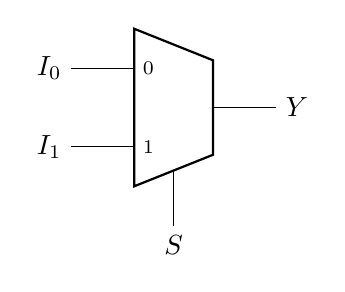
\begin{tikzpicture}
  \muxtwo{m}{(0,0)}{}
  \draw (m-in0) -- ++(-0.8,0) node[left]{$I_0$};
  \draw (m-in1) -- ++(-0.8,0) node[left]{$I_1$};
  \draw (m-sel) -- ++(0,-0.7) node[below]{$S$};
  \draw (m-out) -- ++(0.8,0) node[right]{$Y$};
\end{tikzpicture}
\hspace{1.5cm}
\begin{tabular}[b]{c|c}
\toprule
$S$ & $Y$ \\
\midrule
0 & $I_0$ \\
1 & $I_1$ \\
\bottomrule
\end{tabular}
\caption{A 2:1 multiplexer. The input marked 0 is chosen when $S = 0$.}
\label{fig:mux}
\end{figure}

Bigger muxes choose among more inputs: a 4:1 mux has 2 select bits, an 8:1 mux has 3, and in general an $N$:1 mux needs $\log_2 N$ select bits. Muxes are everywhere in hardware: choosing which register feeds an adder, which input a pipeline stage takes, which data a cache returns.

\section{Building any gate from a 2:1 multiplexer}
\label{sec:muxgates}

Here is the method that answers every ``build X from muxes'' question. Any function $F$ can be split on any one of its variables, say $S$:
\[
  F = \nt{S}\cdot F\big|_{S=0} \;+\; S\cdot F\big|_{S=1}
\]
This is \term{Shannon expansion}. Compare it with the mux equation $Y = \nt{S}\,I_0 + S\,I_1$: they have the same shape. So:

\begin{bigidea}
To build $F$ from a 2:1 mux, pick one variable for the select line. Feed $I_0$ with what $F$ equals when that variable is 0, and feed $I_1$ with what $F$ equals when it is 1.
\end{bigidea}

\begin{worked}{an OR gate from one 2:1 mux}
Build $F = A + B$. Choose $B$ as the select.
\begin{itemize}
  \item When $B = 0$: $F = A + 0 = A$. So $I_0 = A$.
  \item When $B = 1$: $F = A + 1 = 1$. So $I_1 = 1$.
\end{itemize}
Result: $S = B$, $I_0 = A$, $I_1 = 1$. Check: $Y = \nt{B}A + B\cdot1 = \nt{B}A + B = A + B$ (by the rule $X + \nt{X}Y = X + Y$).

Choosing $A$ as the select instead gives $S = A$, $I_0 = B$, $I_1 = 1$, which is equally correct, because OR treats its two inputs the same way.
\end{worked}

\begin{onoa}
The question ``build an OR gate from a 2:1 mux'' was on the Ignite hardware assessment, with the two answers in the worked example above (both are valid). Interviews have also asked for AND and OR from 2:1 muxes, and for XOR from 2:1 muxes, covered next.
\end{onoa}

Applying the method to the other gates (assuming the constants 0 and 1 are available):

\begin{center}
\begin{tabular}{lcccc}
\toprule
Function & $S$ & $I_0$ & $I_1$ & 2:1 muxes needed \\
\midrule
Buffer ($A$) & $A$ & 0 & 1 & 1 \\
NOT ($\nt{A}$) & $A$ & 1 & 0 & 1 \\
AND ($AB$) & $A$ & 0 & $B$ & 1 \\
OR ($A + B$) & $A$ & $B$ & 1 & 1 \\
NAND ($\nt{AB}$) & $A$ & 1 & $\nt{B}$ & 2 (one to make $\nt{B}$) \\
NOR ($\nt{A+B}$) & $A$ & $\nt{B}$ & 0 & 2 \\
XOR ($A \oplus B$) & $A$ & $B$ & $\nt{B}$ & 2 \\
XNOR & $A$ & $\nt{B}$ & $B$ & 2 \\
\bottomrule
\end{tabular}
\end{center}

\begin{worked}{XOR from 2:1 multiplexers}
$A \oplus B$ split on $A$: when $A = 0$ it equals $B$; when $A = 1$ it equals $\nt{B}$. So the main mux has $S = A$, $I_0 = B$, $I_1 = \nt{B}$. If $\nt{B}$ is not available as an input, make it with a second mux wired as an inverter ($S = B$, $I_0 = 1$, $I_1 = 0$). Total: two 2:1 muxes (Figure~\ref{fig:muxxor}).
\end{worked}

\begin{figure}[h]
\centering
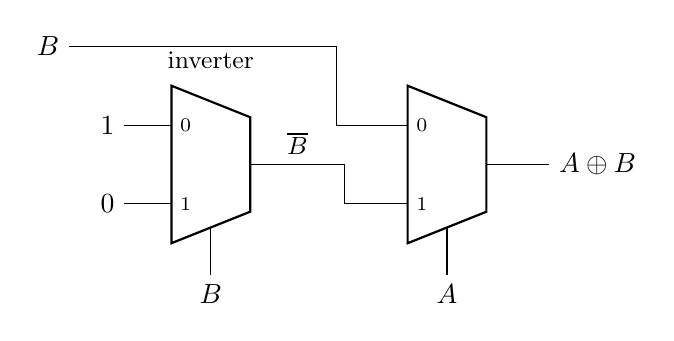
\begin{tikzpicture}
  \muxtwo{a}{(0,0)}{}
  \draw (a-in0) -- ++(-0.6,0) node[left]{1};
  \draw (a-in1) -- ++(-0.6,0) node[left]{0};
  \draw (a-sel) -- ++(0,-0.6) node[below]{$B$};
  \node[above] at (0.5,2.1) {\small inverter};
  \muxtwo{b}{(3,0)}{}
  \draw (a-out) -- node[above,font=\small]{$\nt{B}$} ++(1.2,0) |- (b-in1);
  \draw (b-in0) -- ++(-0.9,0) |- ++(0,1.0) -- ++(-3.4,0) node[left]{$B$};
  \draw (b-sel) -- ++(0,-0.6) node[below]{$A$};
  \draw (b-out) -- ++(0.8,0) node[right]{$A \oplus B$};
\end{tikzpicture}
\caption{XOR from two 2:1 muxes: the first makes $\nt{B}$, the second selects $B$ or $\nt{B}$ based on $A$.}
\label{fig:muxxor}
\end{figure}

\paragraph{Larger muxes from smaller ones.} A 4:1 mux is three 2:1 muxes: two pick within pairs using the low select bit, and a third picks between their outputs using the high select bit. An 8:1 mux takes seven 2:1 muxes. In general, an $N$:1 mux takes $N - 1$ two-input muxes arranged as a tree.

\paragraph{Any function from a bigger mux.} A $2^n$:1 mux with the $n$ inputs on its selects can implement \emph{any} $n$-input function: just put the function's truth-table output values (0s and 1s) on the data inputs. That is exactly a \term{lookup table} (LUT), the basic element of an FPGA. With one more trick, a 4:1 mux implements any 3-input function: put two inputs on the selects and feed each data input with 0, 1, $C$ or $\nt{C}$.

\begin{worked}{majority function from a 4:1 mux}
The 3-input majority function is 1 when at least two inputs are 1. Use $A$ and $B$ as selects:
$AB = 00$: majority needs both others, impossible, so feed 0.
$AB = 01$ or $10$: majority iff $C = 1$, so feed $C$.
$AB = 11$: already a majority, so feed 1.
\end{worked}

Muxes can also build \emph{memory}: a mux whose output is fed back to one of its inputs is a latch. That leads to building flip-flops from muxes in Chapter~\ref{ch:latch}.

\section{Decoders, encoders and demultiplexers}

A \term{decoder} takes an $n$-bit binary number and raises exactly one of its $2^n$ outputs: a 2-to-4 decoder with input $11$ raises output 3. Decoders select memory rows: a memory with 1024 rows uses a 10-to-1024 decoder on its address bits (Chapter~\ref{ch:memory}).

An \term{encoder} does the reverse: given which one of $2^n$ inputs is active, it outputs that input's number. A \term{priority encoder} handles several active inputs by reporting the highest-priority one, which is useful for interrupt controllers and arbiters.

A \term{demultiplexer} routes one input to one of several outputs, chosen by select bits: the opposite of a mux.

\section{Adding binary numbers}

\paragraph{Half adder.} Adding two bits gives a sum bit and a carry bit:
\[
  S = A \oplus B, \qquad C = AB.
\]

\paragraph{Full adder.} To add multi-bit numbers, each position must also add the carry from the position to its right. A \term{full adder} adds three bits, $A$, $B$ and carry-in $C_{in}$:
\[
  S = A \oplus B \oplus C_{in}, \qquad C_{out} = AB + C_{in}(A \oplus B).
\]
$C_{out}$ is the \term{majority} function: it is 1 when at least two of the three inputs are 1. The sum is 1 when an odd number of inputs are 1.

\paragraph{Ripple-carry adder.} Chain $n$ full adders, each passing its carry to the next. It is simple and small, but slow: in the worst case (for example, adding 1 to $0111\ldots1$) a carry must ripple through every stage, so delay grows in proportion to $n$.

\paragraph{Faster adders.} Each position can be described by whether it \term{generates} a carry ($G = AB$: both bits are 1) or \term{propagates} an incoming carry ($P = A \oplus B$: exactly one bit is 1). A \term{carry-lookahead} adder computes the carries for many positions at once from $G$ and $P$ instead of waiting for the ripple. Tree-shaped \term{prefix adders} (such as Kogge--Stone) bring the delay down to grow with $\log_2 n$ instead of $n$, at the cost of more area and wiring. A \term{carry-select} adder computes the upper half twice, once assuming carry-in 0 and once assuming 1, then uses a mux to pick the right one when the real carry arrives.

\paragraph{Subtraction.} Using two's complement (Chapter~\ref{ch:binary}), $A - B = A + \nt{B} + 1$. An adder becomes a subtractor by inverting $B$ (XOR gates controlled by a ``subtract'' signal act as optional inverters) and setting the carry-in to 1.

\paragraph{Comparators.} Two numbers are equal when every bit pair is equal: XNOR each pair, then AND all the results. To find which is larger, subtract and look at the sign or the carry.

\paragraph{Shifters and multipliers.} A \term{barrel shifter} shifts by any amount in one step using layers of muxes (shift by 1, 2, 4, 8, \ldots, each layer enabled or not). A \term{multiplier} adds up shifted copies of one operand (one for each 1 bit in the other); fast multipliers add the partial products with trees of adders. Multipliers are among the largest arithmetic blocks, and a GPU contains thousands of them.

\section{XOR chains and parity}
\label{sec:xorchain}

Because XOR with 1 inverts and XOR with 0 passes, a chain of XOR gates is easy to analyze if you track what each stage does.

\begin{worked}{a chain of 50 XOR gates}
Gate 1 has inputs 1 and $X$. Every later gate $k$ has inputs (output of gate $k-1$) and $X$. What does each gate output?
\begin{itemize}
  \item Gate 1: $1 \oplus X = \nt{X}$.
  \item Gate 2: $\nt{X} \oplus X = 1$.
  \item Gate 3: $1 \oplus X = \nt{X}$.
\end{itemize}
The pattern repeats: odd-numbered gates output $\nt{X}$ and even-numbered gates output 1. Gate 50 outputs 1. Gate 49 outputs $\nt{X}$, so gate 49 followed by an inverter gives $X$.
\end{worked}

\begin{onoa}
A reported question gave a chain of 50 XOR gates with input $X$ and asked for the output of the $N$th gate and the inverted output of the $(N+1)$th gate. The exact wiring may differ from this example, but the method is the same: compute the first two or three stages, spot the period-2 pattern, and use whether $N$ is odd or even.
\end{onoa}

The XOR of many bits is their \term{parity}. Parity bits detect single-bit errors in memory and communication. A parity tree of XOR gates computes the parity of $n$ bits in about $\log_2 n$ gate delays.

\section{Delay through combinational logic}
\label{sec:combdelay}

Gates are not instant: each takes time to charge its output capacitance (Chapter~\ref{ch:capind}). Two numbers describe a gate's timing:

\begin{itemize}
  \item \term{Propagation delay} $t_{pd}$: the \emph{longest} time from an input change until the output has settled to its final value.
  \item \term{Contamination delay} $t_{cd}$: the \emph{shortest} time from an input change until the output \emph{starts} to change.
\end{itemize}

A gate may have different delays for a rising output and a falling output ($t_{pLH}$ and $t_{pHL}$), because the PMOS pull-up and NMOS pull-down have different strengths. The delay of a whole circuit is found by adding delays along each path from input to output. The slowest path is the \term{critical path}; it sets the circuit's propagation delay. The fastest path sets its contamination delay. Both matter for timing (Chapter~\ref{ch:timing}).

\begin{worked}{how long does the output stay at 0?}
$Z = A \cdot \nt{B}$, where $\nt{B}$ comes from an inverter. Delays: inverter rise 2\,ns and fall 1\,ns; AND gate rise 3\,ns and fall 2\,ns. Initially $A = 0$, $B = 1$, so $\nt{B} = 0$ and $Z = 0$. At $t = 0$ both inputs flip: $A$ becomes 1 and $B$ becomes 0. When does $Z$ become 1?

$A$ is high from $t = 0$. The inverter output rises (0 to 1), which takes its \emph{rise} delay: $\nt{B}$ is high at $t = 2$\,ns. The AND gate's inputs are both high only from $t = 2$, and its output rises after its rise delay: $Z$ becomes 1 at $t = 2 + 3 = 5$\,ns. So $Z$ stays at 0 for 5\,ns.
\end{worked}

\begin{onoa}
Reported questions give a small gate circuit with rise and fall delays, flip the inputs at $t = 0$, and ask how long the output stays at a value. The method: walk forward from the inputs, at each gate note which input arrives last for the transition that matters, and add the gate's rise or fall delay according to the direction its output moves.
\end{onoa}

\subsection*{Glitches and hazards}

Unequal path delays can produce a brief wrong pulse, a \term{glitch}, even when the output should not change at all.

\begin{worked}{a glitch}
$Z = A + \nt{A}$ should always be 1. Build $\nt{A}$ with an inverter of delay 1\,ns, and suppose $A$ falls from 1 to 0 at $t = 0$. From $t = 0$ to $t = 1$\,ns, $A$ is already 0 but $\nt{A}$ has not yet risen. Both OR inputs are 0, so after the OR gate's delay, $Z$ dips to 0 for about 1\,ns before returning to 1.
\end{worked}

This is a \term{static-1 hazard}: an output that should stay 1 briefly drops to 0. In a K-map it appears when two groups of 1s touch but do not overlap; adding the redundant \emph{consensus} term that covers the boundary removes the hazard. In synchronous designs (Chapter~\ref{ch:timing}), glitches are usually harmless as long as everything settles before the next clock edge, but they waste power, and a glitch on a clock or an asynchronous reset is a serious bug.

\section{Summary}

\begin{itemize}
  \item NAND and NOR are each universal. OR from NANDs takes 3 gates; XOR takes 4.
  \item A 2:1 mux computes $Y = \nt{S}I_0 + SI_1$. Shannon expansion builds any function from muxes: select on a variable, feed each data input with the function's value for that select value.
  \item OR: $S = B$, $I_0 = A$, $I_1 = 1$. AND: $S = A$, $I_0 = 0$, $I_1 = B$. NOT: $S = A$, $I_0 = 1$, $I_1 = 0$. XOR: $S = A$, $I_0 = B$, $I_1 = \nt{B}$ (two muxes).
  \item $N$:1 mux $= N - 1$ two-input muxes. A $2^n$:1 mux is a lookup table for any $n$-input function.
  \item Full adder: $S = A\oplus B\oplus C_{in}$, $C_{out} = $ majority. Ripple carry is $O(n)$; lookahead and prefix adders are $O(\log n)$. Subtract with $A + \nt{B} + 1$.
  \item XOR chains alternate; track the pattern and the parity of $N$.
  \item Propagation delay is the slowest path; contamination delay the fastest. Unequal paths cause glitches.
\end{itemize}

\section{Exercises}

\begin{enumerate}
  \item Give the $S$, $I_0$ and $I_1$ connections that make a 2:1 mux act as NOT, AND and OR.
  \item How many 2:1 muxes are needed for XOR if $\nt{B}$ is not available? For NAND?
  \item How many 2:1 muxes make a 4:1 mux? An 8:1 mux?
  \item Implement the 3-input majority function with a 4:1 mux using $A$ and $B$ as selects.
  \item A 32-bit ripple-carry adder's full adders each have a 50\,ps carry delay. Estimate the worst-case carry delay.
  \item Compute $5 - 3$ in 4-bit two's complement using addition.
  \item In the 50-gate XOR chain of Section~\ref{sec:xorchain}, what is the output of gate 37? Of gate 37 followed by an inverter?
  \item $Z = A + \nt{A}$, inverter delay 1\,ns. Does $Z$ glitch when $A$ \emph{rises} from 0 to 1? Explain.
  \item In the worked example $Z = A\nt{B}$ (inverter rise 2, fall 1; AND rise 3, fall 2), the inputs now flip back: at $t = 0$, $A$ falls to 0 and $B$ rises to 1. When does $Z$ fall to 0?
  \item How many outputs does a 3-to-8 decoder have? What size decoder selects one of 1024 memory rows?
\end{enumerate}

\subsection*{Answers}
\begin{enumerate}
  \item NOT: $S = A$, $I_0 = 1$, $I_1 = 0$. AND: $S = A$, $I_0 = 0$, $I_1 = B$. OR: $S = A$, $I_0 = B$, $I_1 = 1$ (or $S = B$, $I_0 = A$, $I_1 = 1$).
  \item XOR: 2 (one makes $\nt{B}$). NAND: 2 ($S = A$, $I_0 = 1$, $I_1 = \nt{B}$, with a second mux making $\nt{B}$).
  \item 3; 7.
  \item Data inputs for $AB = 00, 01, 10, 11$: $0, C, C, 1$.
  \item $32 \times 50 = 1600$\,ps $= 1.6$\,ns.
  \item $0101 + \nt{0011} + 1 = 0101 + 1100 + 1 = 1\,0010$. Drop the carry out: $0010 = 2$.
  \item Gate 37 is odd, so it outputs $\nt{X}$; inverted, $X$.
  \item No. When $A$ rises, the OR gate sees $A = 1$ immediately, which already makes $Z = 1$; $\nt{A}$ falling later does not matter. The glitch happens only when $A$ falls.
  \item $Z$ falls as soon as either AND input falls. $A$ falls at $t = 0$; $\nt{B}$ falls at $t = 1$\,ns (inverter fall delay). The earliest falling input is $A$ at $t = 0$, so $Z$ falls after the AND gate's fall delay: $t = 2$\,ns.
  \item 8 outputs. A 10-to-1024 decoder.
\end{enumerate}


\part{Memory and Time}
\chapter{Latches and Flip-Flops}
\label{ch:latch}

Combinational circuits forget: the moment their inputs change, their old outputs are gone. But a computer must remember things: the value in a register, the count in a counter, which step a machine is on. This chapter builds memory out of gates. It explains latches and flip-flops, the difference between them (an assessment question), how to build a flip-flop from multiplexers (an interview question), and the strange behavior called metastability.

\section{Memory from feedback}

Connect two inverters in a loop: the output of the first drives the second, and the output of the second drives the first (Figure~\ref{fig:bistable}).

\begin{figure}[h]
\centering
\begin{circuitikz}
  \draw (0,0) node[not port](a){};
  \draw (0,-1.6) node[not port, xscale=-1](b){};
  \draw (a.out) -- ++(0.5,0) coordinate(q) |- (b.in);
  \draw (b.out) -- ++(-0.5,0) |- (a.in);
  \node[right] at (q) {$Q$};
  \node[left] at ($(b.out)+(-0.5,0.8)$) {$\nt{Q}$};
\end{circuitikz}
\caption{Two cross-coupled inverters: a circuit with two stable states.}
\label{fig:bistable}
\end{figure}

If $Q = 1$, the lower inverter makes $\nt{Q} = 0$, and the upper inverter turns that back into $Q = 1$. The loop holds itself. If $Q = 0$, the same reasoning shows the loop holds that too. The circuit is \term{bistable}: it has two stable states and stays in whichever one it is put in, as long as power is on. That is one bit of memory.

\begin{everyday}
A light switch is bistable: push it up and it stays up, push it down and it stays down. A doorbell button is not: it only stays pressed while you hold it. Memory circuits are the light-switch kind.
\end{everyday}

The remaining problem is how to \emph{write} a new value into the loop. Every latch and flip-flop is a bistable loop plus some way to control when it accepts new data.

\section{The SR latch}

Replace the two inverters with two NOR gates, giving each a spare input: $S$ (set) and $R$ (reset). This is the \term{SR latch} (Figure~\ref{fig:srlatch}).

\begin{figure}[h]
\centering
\begin{circuitikz}
  \draw (0,0) node[nor port](n1){};
  \draw (0,-2.4) node[nor port](n2){};
  \draw (n1.in 1) -- ++(-0.8,0) node[left]{$R$};
  \draw (n2.in 2) -- ++(-0.8,0) node[left]{$S$};
  \draw (n1.out) -- ++(0.8,0) coordinate(q) node[right]{$Q$};
  \draw (n2.out) -- ++(0.8,0) coordinate(qb) node[right]{$\nt{Q}$};
  \draw ($(n1.out)+(0.4,0)$) -- ++(0,-0.7) -- ++(-2.2,-0.6) |- (n2.in 1);
  \draw ($(n2.out)+(0.4,0)$) -- ++(0,0.7) -- ++(-2.2,0.6) |- (n1.in 2);
\end{circuitikz}
\caption{An SR latch made of two cross-coupled NOR gates.}
\label{fig:srlatch}
\end{figure}

Recall that a NOR outputs 0 whenever any input is 1.
\begin{center}
\begin{tabular}{cc|l}
\toprule
$S$ & $R$ & Result \\
\midrule
0 & 0 & hold: $Q$ keeps its previous value \\
1 & 0 & set: $Q = 1$ \\
0 & 1 & reset: $Q = 0$ \\
1 & 1 & forbidden: both outputs forced to 0 \\
\bottomrule
\end{tabular}
\end{center}

$S = R = 1$ is forbidden for two reasons: $Q$ and $\nt{Q}$ are both 0, so they are no longer opposites; and if $S$ and $R$ then drop to 0 at the same moment, the latch races to an unpredictable state. An SR latch built from NAND gates works the same way with active-low inputs ($\nt{S}$ and $\nt{R}$, where 0 means ``do it'').

\section{The D latch}

The SR latch has two awkward inputs and a forbidden case. The \term{D latch} fixes both. It has a data input $D$ and an enable $EN$ (often the clock):
\begin{itemize}
  \item While $EN = 1$, the latch is \term{transparent}: $Q$ follows $D$, changing whenever $D$ changes.
  \item While $EN = 0$, the latch is \term{opaque}: $Q$ holds whatever value $D$ had at the moment $EN$ fell.
\end{itemize}

The simplest way to build one is a 2:1 mux whose output feeds back to one of its own inputs:
\[
  Q = EN\;?\;D : Q.
\]
When $EN = 1$ the mux passes $D$; when $EN = 0$ it passes its own output back to itself, a loop that holds the value (Figure~\ref{fig:muxlatch}). In transistor-level designs, the mux is made of two transmission gates, one letting $D$ in and one closing the feedback loop of two inverters.

\begin{figure}[h]
\centering
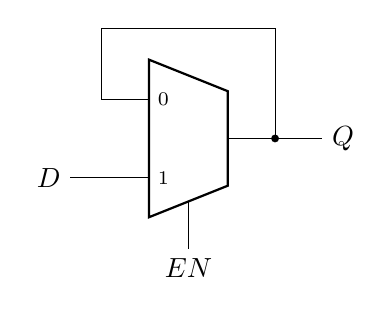
\begin{tikzpicture}
  \muxtwo{m}{(0,0)}{}
  \draw (m-in1) -- ++(-1.0,0) node[left]{$D$};
  \draw (m-sel) -- ++(0,-0.6) node[below]{$EN$};
  \draw (m-out) -- ++(1.2,0) coordinate(q) node[right]{$Q$};
  \draw ($(m-out)+(0.6,0)$) -- ++(0,1.4) -- ++(-2.2,0) |- (m-in0);
  \fill ($(m-out)+(0.6,0)$) circle (0.05);
\end{tikzpicture}
\caption{A D latch from a 2:1 mux. The 1 input takes new data; the 0 input feeds the output back to hold it.}
\label{fig:muxlatch}
\end{figure}

\begin{figure}[h]
\centering
\begin{tikztimingtable}[timing/slope=0.05, xscale=1.6, yscale=1.2]
$EN$ & LL HHHH LLLL HHHH LL \\
$D$  & L HHH LL HH LL LLL HHH \\
$Q$  & LL HH LL LLLL LLL HHH \\
\extracode
\begin{pgfonlayer}{background}
\vertlines[help lines]{2,6,10,14}
\end{pgfonlayer}
\end{tikztimingtable}
\caption{A D latch: while $EN$ is high, $Q$ follows $D$; while $EN$ is low, $Q$ holds (the pulse on $D$ during the low phase never reaches $Q$).}
\label{fig:latchtiming}
\end{figure}

\section{The edge-triggered D flip-flop}

A latch is transparent for the whole time its enable is high, which makes timing hard to control (we will see why shortly). Usually we want a storage element that captures its input at one precise instant, the moment the clock rises, and ignores the input at all other times. That is the \term{D flip-flop}.

\paragraph{Master--slave construction.} Put two D latches in a row with opposite enables (Figure~\ref{fig:masterslave}):
\begin{itemize}
  \item the \term{master} latch is transparent while $CLK = 0$;
  \item the \term{slave} latch is transparent while $CLK = 1$.
\end{itemize}

\begin{figure}[h]
\centering
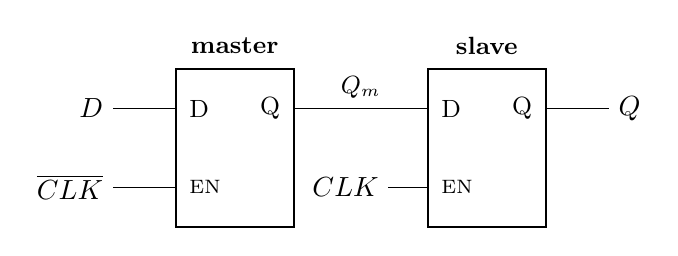
\begin{tikzpicture}
  \dbox{m}{(0,0)}{master}{0}
  \dbox{s}{(3.2,0)}{slave}{0}
  \draw (m-d) -- ++(-0.8,0) node[left]{$D$};
  \draw (m-q) -- node[above,font=\small]{$Q_m$} (s-d);
  \draw (s-q) -- ++(0.8,0) node[right]{$Q$};
  \draw (m-clk) -- ++(-0.8,0) node[left]{$\nt{CLK}$};
  \draw (s-clk) -- ++(-0.5,0) node[left]{$CLK$};
\end{tikzpicture}
\caption{A positive-edge-triggered D flip-flop: master latch enabled by $\nt{CLK}$, slave latch enabled by $CLK$.}
\label{fig:masterslave}
\end{figure}

Step through one clock cycle:
\begin{enumerate}
  \item \textbf{While $CLK = 0$:} the master is transparent, so $Q_m$ follows $D$. The slave is opaque, so $Q$ holds its old value.
  \item \textbf{At the rising edge:} the master closes, freezing $Q_m$ at the value $D$ had at that instant. At the same moment the slave opens and passes that frozen value to $Q$.
  \item \textbf{While $CLK = 1$:} the master is closed, so changes on $D$ cannot get in. The slave is transparent, but its input $Q_m$ is frozen, so $Q$ stays put.
\end{enumerate}
The net effect: $Q$ takes the value of $D$ at each rising clock edge and holds it for the rest of the cycle. At no time is there a transparent path all the way from $D$ to $Q$.

\begin{figure}[h]
\centering
\begin{tikztimingtable}[timing/slope=0.05, xscale=1.6, yscale=1.2]
$CLK$ & LL HH LL HH LL HH LL HH \\
$D$   & L HH L H LLLL HHHH LLL \\
$Q$   & LL HHHH LLLL HHHH LL \\
\extracode
\begin{pgfonlayer}{background}
\vertlines[help lines]{2,6,10,14}
\end{pgfonlayer}
\end{tikztimingtable}
\caption{A D flip-flop: $Q$ changes only at rising clock edges (gridlines), taking the value $D$ had at that instant. The brief dip in $D$ between edges is ignored.}
\label{fig:fftiming}
\end{figure}

\section{A D flip-flop from two 2:1 multiplexers}
\label{sec:ffmux}

Since a D latch is one mux with feedback, a flip-flop is two of them:

\begin{itemize}
  \item \textbf{Master mux:} $S = CLK$, $I_0 = D$, $I_1 = Q_m$ (its own output fed back). It is transparent when $CLK = 0$ and holds when $CLK = 1$.
  \item \textbf{Slave mux:} $S = CLK$, $I_0 = Q$ (its own output fed back), $I_1 = Q_m$. It holds when $CLK = 0$ and is transparent when $CLK = 1$.
\end{itemize}

\begin{figure}[h]
\centering
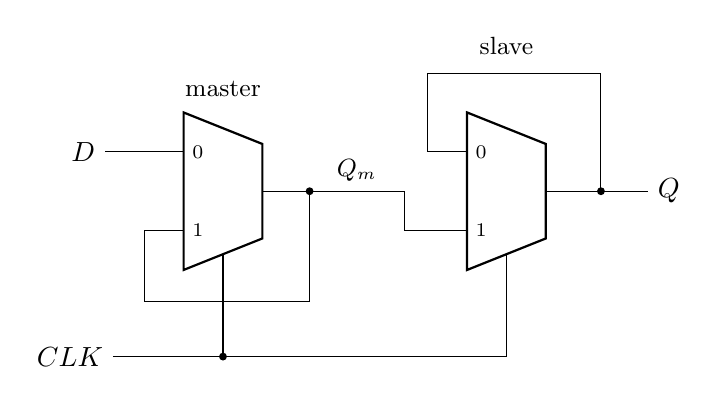
\begin{tikzpicture}
  \muxtwo{a}{(0,0)}{}
  \muxtwo{b}{(3.6,0)}{}
  \draw (a-in0) -- ++(-1.0,0) node[left]{$D$};
  % master feedback into in1
  \draw (a-out) -- ++(0.6,0) coordinate(am);
  \fill (am) circle (0.05);
  \draw (am) |- ($(a-in1)+(-0.5,-0.9)$) |- (a-in1);
  % master to slave in1
  \draw (am) -- ++(1.2,0) |- (b-in1);
  \node[above,font=\small] at ($(am)+(0.6,0)$) {$Q_m$};
  % slave feedback into in0
  \draw (b-out) -- ++(0.7,0) coordinate(bq);
  \fill (bq) circle (0.05);
  \draw (bq) |- ($(b-in0)+(-0.5,1.0)$) |- (b-in0);
  \draw (bq) -- ++(0.6,0) node[right]{$Q$};
  % clock
  \draw (a-sel) -- ++(0,-1.3) coordinate(ca);
  \draw (b-sel) -- ++(0,-1.3) coordinate(cb);
  \draw ($(ca)+(-1.4,0)$) node[left]{$CLK$} -- (cb);
  \fill (ca) circle (0.05);
  \node[font=\small] at (0.5,2.3) {master};
  \node[font=\small] at (4.1,2.85) {slave};
\end{tikzpicture}
\caption{A positive-edge D flip-flop from two 2:1 muxes. Both selects are driven by $CLK$; the feedback goes to opposite data inputs, so the two latches are transparent in opposite clock phases.}
\label{fig:ffmux}
\end{figure}

\begin{onoa}
Interview reports include ``make a D flip-flop using 2:1 muxes.'' The answer is Figure~\ref{fig:ffmux}: two mux-latches in series, enabled in opposite clock phases. (Moving the feedback to the other input of each mux gives a negative-edge flip-flop.) In real silicon, care is needed so that both latches are never transparent at the same time during the clock transition, but the logical structure is exactly this.
\end{onoa}

\section{Latch versus flip-flop}
\label{sec:latchvsff}

\begin{center}
\begin{tabularx}{\linewidth}{>{\raggedright\arraybackslash}p{3.2cm}>{\raggedright\arraybackslash}X>{\raggedright\arraybackslash}X}
\toprule
 & Latch & Flip-flop \\
\midrule
Triggered by & clock \textbf{level} & clock \textbf{edge} \\
While the clock is active & transparent: output follows input & opaque: input only sampled at the edge \\
Size & one latch (smaller) & two latches (about twice the size) \\
Power & lower & higher (more transistors, more clock load) \\
Glitches on the input & passed through while transparent & ignored except near the edge \\
Timing & harder: data can race through; but allows time borrowing & simpler: one capture per cycle \\
\bottomrule
\end{tabularx}
\end{center}

\begin{onoa}
``What is one advantage of a flip-flop over a latch?'' was an Ignite assessment question. The key answer: \textbf{a flip-flop is edge-triggered, so it samples its input at one instant per cycle and is never transparent.} Data cannot ``race through'' several stages in one clock phase, glitches on the input are ignored, and timing analysis is simple and predictable. Advantages of a latch in return: it is smaller, uses less power, and allows \emph{time borrowing} (a slow stage can use some of the next stage's time while the latch is transparent, Chapter~\ref{ch:timing}).
\end{onoa}

\paragraph{Why race-through is a problem.} Imagine a pipeline of latches all enabled by the same clock. While the clock is high, every latch is transparent at once, and data entering the first latch can rush through the logic and into the second, third and fourth before the clock falls. The circuit no longer advances one step per cycle; it advances an unpredictable number of steps depending on gate delays. Flip-flops cannot do this, because no flip-flop is ever transparent from input to output. (Latch-based designs avoid the problem by alternating latches on opposite clock phases, which is exactly what a master--slave flip-flop does internally.)

\section{Other kinds of flip-flop}

Older textbooks and some interview questions use other flip-flop types. Each can be built from a D flip-flop plus a little logic.

\begin{center}
\begin{tabular}{lll}
\toprule
Type & Behavior at the clock edge & Next state $Q^+$ \\
\midrule
D & copy $D$ & $D$ \\
T (toggle) & flip if $T = 1$, hold if $T = 0$ & $T \oplus Q$ \\
JK & $J$ sets, $K$ resets, both 1 toggles, both 0 holds & $J\nt{Q} + \nt{K}Q$ \\
SR & $S$ sets, $R$ resets, both 1 not allowed & $S + \nt{R}Q$ \\
\bottomrule
\end{tabular}
\end{center}

\begin{itemize}
  \item A \textbf{T flip-flop} is a D flip-flop with $D = T \oplus Q$.
  \item A \textbf{T flip-flop with $T = 1$}, or a D flip-flop with $\nt{Q}$ fed back to $D$, toggles on every clock edge. Its output is a square wave at \emph{half} the clock frequency: a divide-by-two circuit (Chapter~\ref{ch:fsm}).
\end{itemize}

\section{Set, reset and enable}

\paragraph{Asynchronous set and clear.} Many flip-flops have extra inputs that force the output immediately, without waiting for a clock edge: \term{preset} (or set) forces $Q = 1$, and \term{clear} (or reset) forces $Q = 0$. These are often \term{active low}, written $\nt{PRE}$ and $\nt{CLR}$: they act when held at 0.

\begin{trap}
``Set and clear tied to zero'' means opposite things depending on the polarity. For \emph{active-high} set and clear, tying them to 0 disables them, and the flip-flop works normally. For \emph{active-low} inputs, tying them to 0 asserts them, and the output is stuck (and with both asserted, the behavior is invalid). Always check whether the input has a bubble on the symbol.
\end{trap}

\paragraph{Synchronous versus asynchronous reset.} An \term{asynchronous} reset acts immediately, even with no clock running. A \term{synchronous} reset is just a condition in the logic in front of $D$, so it takes effect only at the next clock edge. Both are common; Chapter~\ref{ch:rtl} discusses the trade-offs.

\paragraph{Enable.} To make a flip-flop update only when an enable signal is 1, put a mux in front of it: $D_{\text{ff}} = EN\;?\;D : Q$. When disabled, the flip-flop reloads its own value each cycle. (An alternative is to stop its clock, called clock gating, which saves power, Chapter~\ref{ch:power}.)

\paragraph{Scan flip-flops.} Chips are tested after manufacturing by loading known patterns into every flip-flop. A \term{scan flip-flop} has a mux in front that, in test mode, connects all flip-flops into one long shift register (a \term{scan chain}) so test patterns can be shifted in and results shifted out.

\section{Metastability}
\label{sec:metastability}

A flip-flop needs its input to be stable for a short window around the clock edge (the setup and hold times, Chapter~\ref{ch:timing}). What if the input changes inside that window? The bistable loop can be caught balanced exactly between its two states, like a ball balanced on top of a hill. Eventually noise tips it one way or the other, but \emph{how long} that takes is unpredictable. While it hangs there, the output sits at an in-between voltage that is neither a valid 0 nor a valid 1. This is \term{metastability}.

\begin{figure}[h]
\centering
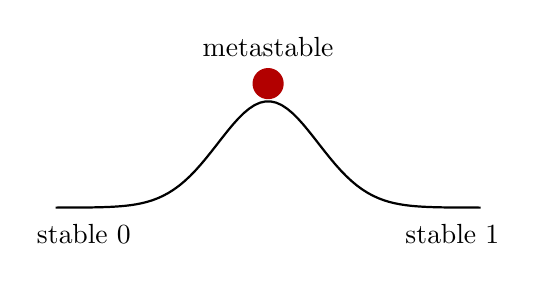
\begin{tikzpicture}[scale=0.9]
  \draw[thick,domain=-3:3,samples=80] plot (\x,{1.5*exp(-\x*\x)});
  \fill[red!70!black] (0,1.75) circle (0.22);
  \node[below] at (-2.6,-0.1) {stable 0};
  \node[below] at (2.6,-0.1) {stable 1};
  \node[above] at (0,2.0) {metastable};
\end{tikzpicture}
\caption{Metastability: a ball balanced on a hill eventually rolls to one side, but nobody can say exactly when.}
\end{figure}

Key facts:
\begin{itemize}
  \item Metastability happens whenever the input is \term{asynchronous}: it comes from outside the flip-flop's clock domain (a button, another chip, a different clock), so it can change at any time.
  \item It \emph{cannot be eliminated}, only made very unlikely.
  \item The probability that the flip-flop is still unresolved after waiting time $t$ falls \emph{exponentially} with $t$. So the mean time between failures (MTBF) grows exponentially with the time you allow it to settle.
  \item The standard defense is a \term{synchronizer}: two flip-flops in a row on the receiving clock. The first may go metastable, but it has a whole clock cycle to resolve before the second samples it. This reduces the failure rate to something like once in thousands of years (Chapter~\ref{ch:rtl}).
\end{itemize}

\section{Summary}

\begin{itemize}
  \item Memory comes from feedback: two cross-coupled inverters are bistable.
  \item SR latch: set, reset, hold; $S = R = 1$ forbidden.
  \item D latch: transparent while enabled, holds while disabled. A 2:1 mux with feedback is a D latch.
  \item D flip-flop: master latch (transparent on $CLK = 0$) plus slave latch (transparent on $CLK = 1$) captures $D$ at the rising edge. Two muxes make one.
  \item Flip-flop advantages: edge-triggered, never transparent, no race-through, glitches ignored, easy timing. Latch advantages: smaller, lower power, time borrowing.
  \item T flip-flop: $Q^+ = T \oplus Q$; with $T = 1$ it divides the clock by 2. JK: $Q^+ = J\nt{Q} + \nt{K}Q$.
  \item Check set/clear polarity before deciding what ``tied to 0'' means.
  \item Metastability cannot be eliminated; synchronizers make it exponentially unlikely.
\end{itemize}

\section{Exercises}

\begin{enumerate}
  \item A NOR SR latch has $S = 1$, $R = 0$. Then $S$ returns to 0. What is $Q$ now?
  \item Why is $S = R = 1$ not allowed in a NOR SR latch?
  \item A D latch has $EN = 1$ and $D$ toggles three times. How many times does $Q$ change? What if $EN = 0$?
  \item Draw (or describe) a D latch made from one 2:1 mux. Which input gets the feedback?
  \item Describe the connections of a positive-edge D flip-flop built from two 2:1 muxes.
  \item State one advantage of a flip-flop over a latch, and one advantage of a latch over a flip-flop.
  \item How do you make a T flip-flop from a D flip-flop?
  \item A JK flip-flop has $J = K = 1$. What does it do on each clock edge?
  \item A flip-flop has active-low asynchronous clear, and the clear input is tied to 0. What is $Q$?
  \item True or false: with careful design, metastability can be completely eliminated.
  \item A D flip-flop is clocked at 100\,MHz with $\nt{Q}$ connected to $D$. What is the frequency of $Q$?
\end{enumerate}

\subsection*{Answers}
\begin{enumerate}
  \item $Q = 1$: the latch was set, and with $S = R = 0$ it holds.
  \item It forces both $Q$ and $\nt{Q}$ to 0 (no longer complements), and if both inputs then return to 0 together, the final state depends on a race and is unpredictable.
  \item Three times (it is transparent; $Q$ follows each change of $D$). With $EN = 0$, zero times.
  \item The mux's select is $EN$; $D$ goes to the 1 input; the output is fed back to the 0 input.
  \item Master mux: select $CLK$, $I_0 = D$, $I_1$ = its own output $Q_m$. Slave mux: select $CLK$, $I_1 = Q_m$, $I_0$ = its own output $Q$.
  \item Flip-flop: edge-triggered, never transparent, so no race-through and simpler timing (also ignores glitches). Latch: smaller and lower power, and allows time borrowing.
  \item Feed $D = T \oplus Q$.
  \item It toggles ($Q^+ = \nt{Q}$).
  \item The clear is permanently asserted, so $Q$ is stuck at 0.
  \item False. Its probability can only be made extremely small.
  \item 50\,MHz (the output toggles once per clock period, so its period is two clock periods).
\end{enumerate}

\chapter{Timing: Setup, Hold and Clock Speed}
\label{ch:timing}

How fast can a chip run? What limits it? Why can one mistake be fixed by slowing the clock while another makes the chip useless at any speed? This chapter answers those questions. Timing is the single most important topic in digital hardware interviews, and it is the foundation for the clock divider, pipeline and FIFO questions later in the book.

\section{Synchronous design}

Almost every digital chip follows one pattern, called \term{synchronous design}: banks of flip-flops (registers) hold the current state, blocks of combinational logic compute the next state from it, and one shared clock tells every flip-flop to capture its new value at the same moment (Figure~\ref{fig:syncpath}).

\begin{figure}[h]
\centering
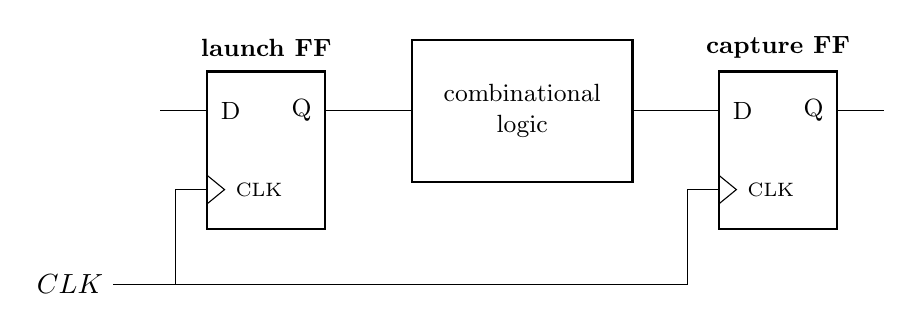
\begin{tikzpicture}
  \dbox{a}{(0,0)}{launch FF}{1}
  \draw[thick] (2.6,0.6) rectangle (5.4,2.4); \node[align=center,font=\small] at (4,1.5) {combinational\\logic};
  \dbox{b}{(6.5,0)}{capture FF}{1}
  \draw (a-q) -- (2.6,1.5); \draw (5.4,1.5) -- (b-d);
  \draw (a-d) -- ++(-0.6,0);
  \draw (b-q) -- ++(0.6,0);
  \draw (a-clk) -- ++(-0.4,0) |- (-0.4,-0.7) -- (6.1,-0.7) |- (b-clk);
  \draw (-0.4,-0.7) -- ++(-0.8,0) node[left]{$CLK$};
\end{tikzpicture}
\caption{The basic timing path: a launch flip-flop, logic, and a capture flip-flop on the same clock.}
\label{fig:syncpath}
\end{figure}

At each rising clock edge, the launch flip-flop sends out a new value. It ripples through the logic. At the \emph{next} rising edge, the capture flip-flop must grab the result. The whole chip advances one step per clock cycle, and as long as every path obeys two timing rules, gate delays never cause errors. Those two rules are the subject of this chapter.

\section{The clock}

A clock is a square wave. Its \term{period} $T$ is the time between rising edges; its \term{frequency} is $f = 1/T$. A 2\,GHz clock has a 500\,ps period. The \term{duty cycle} is the fraction of the period the clock spends high, normally 50\%.

\section{Timing parameters}

Every flip-flop and logic block has a few timing numbers:

\begin{itemize}
  \item \term{Setup time} $t_{su}$: how long \emph{before} the clock edge the input $D$ must be stable.
  \item \term{Hold time} $t_h$: how long \emph{after} the clock edge $D$ must stay stable.
  \item \term{Clock-to-Q delay} $t_{cq}$: how long after the clock edge the output $Q$ changes.
  \item For the logic: the \term{propagation delay} $t_{pd}$ (slowest path, time until the output is final) and the \term{contamination delay} $t_{cd}$ (fastest path, time until the output first starts changing), as in Chapter~\ref{ch:comb}.
\end{itemize}

\begin{figure}[h]
\centering
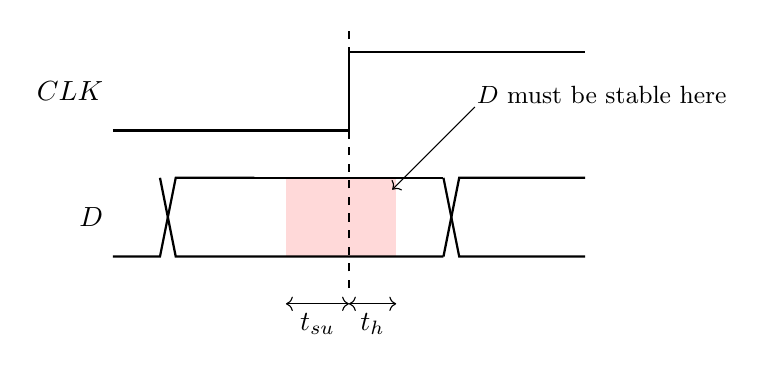
\begin{tikzpicture}[scale=1.0]
  \draw[thick] (0,2) -- (3,2) -- (3,3) -- (6,3);
  \node[left] at (0,2.5) {$CLK$};
  \fill[red!15] (2.2,0.4) rectangle (3.6,1.4);
  \draw[thick] (0,0.4) -- (0.6,0.4) -- (0.8,1.4) -- (1.8,1.4);
  \draw[thick] (1.8,1.4) -- (4.2,1.4);
  \draw[thick] (0.6,1.4) -- (0.8,0.4) -- (1.8,0.4) -- (4.2,0.4);
  \draw[thick] (4.2,0.4) -- (4.4,1.4) -- (6,1.4); \draw[thick] (4.2,1.4) -- (4.4,0.4) -- (6,0.4);
  \node[left] at (0,0.9) {$D$};
  \draw[dashed] (3,0) -- (3,3.3);
  \draw[<->] (2.2,-0.2) -- node[below]{$t_{su}$} (3,-0.2);
  \draw[<->] (3,-0.2) -- node[below]{$t_h$} (3.6,-0.2);
  \node[font=\small,anchor=west] at (4.5,2.45) {$D$ must be stable here};
  \draw[->] (4.6,2.3) -- (3.55,1.25);
\end{tikzpicture}
\caption{$D$ must not change inside the shaded window around the clock edge: from $t_{su}$ before it to $t_h$ after it.}
\label{fig:window}
\end{figure}

If $D$ changes inside that window (Figure~\ref{fig:window}), the flip-flop may capture the wrong value or go metastable (Chapter~\ref{ch:latch}).

\section{The setup constraint: how fast can the clock go?}

Follow the data launched at one clock edge (time 0) to the capture flip-flop.
\begin{enumerate}
  \item The launch flip-flop's output changes at $t_{cq}$.
  \item The change ripples through the logic and settles by $t_{cq} + t_{pd}$.
  \item The capture flip-flop samples at the next edge, time $T$, and needs the data stable $t_{su}$ before that.
\end{enumerate}
So the data must arrive in time:
\[
  \boxed{t_{cq} + t_{pd} + t_{su} \le T}
\]
The minimum period is the sum on the left, and the maximum frequency is its reciprocal:
\[
  f_{max} = \frac{1}{t_{cq} + t_{pd} + t_{su}}.
\]

\begin{bigidea}
The setup constraint is about data arriving \emph{too late}. It is set by the slowest path (the \term{critical path}), and it depends on the clock period. If it fails, you can always fix it by slowing the clock down.
\end{bigidea}

\begin{worked}{maximum clock frequency}
$t_{cq} = 50$\,ps, the slowest logic path $t_{pd} = 400$\,ps, $t_{su} = 30$\,ps.
\[
  T_{min} = 50 + 400 + 30 = 480~\text{ps}, \qquad f_{max} = \frac{1}{480~\text{ps}} \approx 2.08~\text{GHz}.
\]
\end{worked}

\begin{worked}{the logic budget}
A design must run at 500\,MHz ($T = 2$\,ns). Its flip-flops have $t_{cq} = 0.3$\,ns and $t_{su} = 0.2$\,ns. What is the longest the logic may take?
\[
  t_{pd} \le T - t_{cq} - t_{su} = 2 - 0.3 - 0.2 = 1.5~\text{ns}.
\]
\end{worked}

\section{The hold constraint: data arriving too early}

There is a second, sneakier danger. At the same clock edge at which the capture flip-flop samples the \emph{old} data, the launch flip-flop is sending \emph{new} data. If that new data races through a very short path and arrives before the capture flip-flop's hold time is over, it corrupts the value being captured.

The earliest the new data can arrive is $t_{cq} + t_{cd}$ (using the fastest clock-to-Q and the fastest logic path). It must not arrive before the hold window closes:
\[
  \boxed{t_{cq} + t_{cd} \ge t_h}
\]

\begin{bigidea}
The hold constraint involves only \emph{one} clock edge, the same edge launching and capturing, so \textbf{the clock period does not appear in it}. A hold violation cannot be fixed by slowing the clock. A chip with a hold violation fails at every frequency. It is fixed by \emph{adding delay} (buffers) to the too-fast path.
\end{bigidea}

\begin{worked}{a hold violation}
$t_{cq} = 40$\,ps, the shortest logic path is 10\,ps, $t_h = 60$\,ps.
Arrival $= 40 + 10 = 50$\,ps $< 60$\,ps: a hold violation of 10\,ps. Lowering the frequency changes nothing. Add at least 10\,ps of delay on the short path (in practice, a little more for margin).
\end{worked}

\begin{trap}
``The chip fails a timing check; can we fix it by lowering the clock frequency?'' Yes for setup, \emph{no} for hold. This is one of the most common true/false questions. A related trap: adding logic delay \emph{helps} hold and \emph{hurts} setup.
\end{trap}

\section{Clock skew and jitter}

So far we assumed the clock reaches every flip-flop at the same instant. In reality the clock travels through wires and buffers, and different flip-flops receive it at slightly different times. The difference is \term{clock skew}. Define
\[
  t_{skew} = (\text{clock arrival at capture FF}) - (\text{clock arrival at launch FF}).
\]
Positive skew means the capture flip-flop's clock arrives later.

With skew, the constraints become:
\[
  \text{setup: } t_{cq} + t_{pd} + t_{su} \le T + t_{skew}, \qquad
  \text{hold: } t_{cq} + t_{cd} \ge t_h + t_{skew}.
\]

Positive skew gives the data extra time to arrive before the capture edge, which \textbf{helps setup}. But it also keeps the capture flip-flop's hold window open later, which \textbf{hurts hold}. Negative skew does the opposite. Skew is a trade: whatever it gives one constraint, it takes from the other.

\term{Jitter} is random variation in the clock edge timing from cycle to cycle. Because nobody can predict it, it always eats into the margin; for setup, it effectively shortens the period.

\begin{worked}{skew in a clock buffer}
At 500\,MHz, $t_{cq} = 0.3$\,ns, $t_{su} = 0.2$\,ns, and the capture flip-flop's clock passes through one extra buffer of 0.1\,ns, so $t_{skew} = +0.1$\,ns. The logic budget becomes
\[
  t_{pd} \le T + t_{skew} - t_{cq} - t_{su} = 2 + 0.1 - 0.3 - 0.2 = 1.6~\text{ns}.
\]
If the hold time is 0.15\,ns, the shortest path must satisfy $0.3 + t_{cd} \ge 0.15 + 0.1$: true for any $t_{cd} \ge 0$, so hold is safe.
\end{worked}

\section{Slack}

Timing tools report \term{slack}: how much margin a path has.
\[
  \text{setup slack} = (T + t_{skew}) - (t_{cq} + t_{pd} + t_{su}), \qquad
  \text{hold slack} = (t_{cq} + t_{cd}) - (t_h + t_{skew}).
\]
Positive slack means the path passes with that much to spare; negative slack is a violation. \term{Static timing analysis} (STA) tools compute the slack of every path in a chip, using worst-case delays, without simulating any data.

\section{Reading timing diagrams}

Assessment questions often show a waveform and ask for the output. The method:
\begin{enumerate}
  \item Mark every active clock edge (usually rising).
  \item At each edge, read the value of $D$ just \emph{before} the edge (that is what is captured).
  \item Draw $Q$ changing to that value a little after the edge ($t_{cq}$), and holding until the next edge.
  \item For a chain of flip-flops, repeat stage by stage: each stage's input is the previous stage's output, which changed only just after the edge, so each stage sees the \emph{old} value at that edge.
\end{enumerate}

\begin{figure}[h]
\centering
\begin{tikztimingtable}[timing/slope=0.05, xscale=1.5, yscale=1.2]
$CLK$ & LL HH LL HH LL HH LL HH LL \\
$D$   & L HHHH LLL LLLL HHHH LL \\
$Q_1$ & 2.3L 4H 8L 3.7H \\
$Q_2$ & 6.3L 4H 7.7L \\
\extracode
\begin{pgfonlayer}{background}
\vertlines[help lines]{2,6,10,14}
\end{pgfonlayer}
\end{tikztimingtable}
\caption{Two flip-flops in a row ($D \to Q_1 \to Q_2$). Each output changes slightly after a rising edge (gridlines). $Q_2$ copies $Q_1$ one cycle later.}
\label{fig:twoflops}
\end{figure}

\section{Shift registers and hold time}

A \term{shift register} is a chain of flip-flops with each $Q$ wired directly to the next $D$, no logic in between. On each clock edge every bit moves one place along. Because there is no logic, $t_{cd} = 0$, and the hold check is simply $t_{cq} \ge t_h + t_{skew}$.

\begin{worked}{a 4-bit shift register}
Four D flip-flops form a shift register. Each has $t_{cq} = 50$\,ps (positive) and $t_h = 0$.
\begin{itemize}
  \item With zero skew: $50 \ge 0$. Hold is met. Each stage captures its neighbor's old value before the neighbor changes, and the register shifts exactly one place per edge.
  \item Now suppose the clock reaches each flip-flop 60\,ps later than the one before it ($t_{skew} = +60$\,ps along the shift direction). Hold requires $50 \ge 0 + 60$: violated. The new value from one flip-flop arrives at the next one before that one's (late) clock edge, so data can skip through two stages in one cycle and bits are lost.
  \item Fix: route the clock the other way (so skew is negative along the data direction), or add delay between stages.
\end{itemize}
\end{worked}

\begin{onoa}
A reported question describes a 4-bit shift register of D flip-flops with positive clock-to-Q delay and zero hold time. The point being tested: with no logic between stages, correct shifting depends on $t_{cq}$ being larger than the hold time plus any skew. With $t_h = 0$ and no skew, any positive $t_{cq}$ works.
\end{onoa}

\section{Pipelining}
\label{sec:pipelining}

If the critical path is too slow for the clock you want, you can split the logic into stages with registers between them. This is \term{pipelining}.

\begin{worked}{pipelining a slow block}
A 900\,ps block of logic sits between two registers whose overhead is $t_{cq} + t_{su} = 100$\,ps. The clock period must be at least 1000\,ps (1\,GHz). Split the logic into three 300\,ps stages with registers between: each stage needs $300 + 100 = 400$\,ps, so the clock can run at 2.5\,GHz.
\begin{itemize}
  \item \textbf{Throughput} (results per second) rises from 1 to 2.5 billion: a new input enters every 400\,ps.
  \item \textbf{Latency} (time for one input to come out) rises from 1000\,ps to $3 \times 400 = 1200$\,ps.
\end{itemize}
\end{worked}

Pipelining trades latency for throughput. Its returns diminish: each extra stage adds another $t_{cq} + t_{su}$ of overhead, and stages can never be perfectly balanced. Processor pipelines (Chapter~\ref{ch:arch}) are the most famous example.

\section{Long wires and retiming flip-flops}
\label{sec:retiming}

On a large chip, just sending a signal across the die can take longer than a clock period. The fix is the same idea as pipelining: insert flip-flops along the wire so that each segment fits in one cycle. These are sometimes called \term{pipeline} or \term{retiming flops}.

\begin{worked}{flip-flops on a long wire}
A signal must travel 60\,mm between two flip-flops. The wire (with repeaters) has a delay of 0.1\,ns per mm. The clock period is 5\,ns, and each flip-flop's overhead is $t_{cq} + t_{su} = 0.2$\,ns. Assume the clock arrives everywhere at the same time.

Total wire delay: $60 \times 0.1 = 6$\,ns, longer than one period. Each segment can use at most $5 - 0.2 = 4.8$\,ns, which covers $4.8/0.1 = 48$\,mm. Segments needed: $\lceil 60/48 \rceil = 2$. Two segments need \textbf{one} extra flip-flop in the middle. The signal now takes two cycles to arrive.
\end{worked}

\begin{onoa}
A reported question gives two flip-flops 60\,mm apart, data and clock wire delays, and a 5\,ns period, and asks for the minimum number of retiming flip-flops. If the clock is routed along with the data, its wire delay creates skew: add the skew to the time each segment may use (positive skew in the data direction helps setup). Then divide the total data delay by the time per segment, round up to get segments, and subtract one to get flip-flops.
\end{onoa}

\section{Time borrowing with latches}

Latch-based designs can do something flip-flop designs cannot. Because a latch is transparent for a whole clock phase, data that arrives late at a latch is not lost; it passes through while the latch is open, and the next stage simply starts late. A slow stage can \term{borrow time} from a fast one that follows it. This is one reason high-performance custom designs sometimes use latches instead of flip-flops, despite their harder timing analysis.

\section{Special paths and sign-off corners}

\begin{itemize}
  \item A \term{false path} is a path that exists in the wiring but can never actually carry a meaningful transition (for example, through two muxes whose selects are never set that way together). It is excluded from timing checks.
  \item A \term{multicycle path} is allowed more than one clock cycle by design (for example, a slow divider whose result is only read every other cycle).
  \item Timing must be met across manufacturing and operating variation (Chapter~\ref{ch:pvt}). \textbf{Setup} is checked at the \textbf{slow} corner (slow transistors, low voltage, worst temperature), where paths are longest. \textbf{Hold} is checked at the \textbf{fast} corner, where short paths are shortest.
\end{itemize}

\section{Making and distributing the clock}

\begin{itemize}
  \item A \term{phase-locked loop} (PLL) generates a fast, stable clock from a slower reference crystal, by multiplying its frequency.
  \item A \term{clock tree} distributes the clock to millions of flip-flops through a balanced network of buffers (H-trees, meshes, spines) designed to keep skew small.
  \item \term{Clock gating} turns off the clock to idle flip-flops to save power (Chapter~\ref{ch:power}). It must be done with a special cell (a latch plus an AND gate) so the gated clock never glitches.
  \item A group of flip-flops driven by one clock forms a \term{clock domain}. Signals that cross between domains need special handling (Chapter~\ref{ch:rtl}).
\end{itemize}

\section{Summary}

\begin{itemize}
  \item Setup: $t_{cq} + t_{pd} + t_{su} \le T + t_{skew}$. It limits frequency; fix it by slowing the clock, shortening logic, or pipelining.
  \item Hold: $t_{cq} + t_{cd} \ge t_h + t_{skew}$. No $T$ in it; fix it by adding delay, never by slowing the clock.
  \item Positive skew (capture clock late) helps setup and hurts hold.
  \item Slack is the margin; negative slack is a violation.
  \item In a timing diagram, each flip-flop captures the value just before the edge and changes $t_{cq}$ after it.
  \item Shift registers depend on $t_{cq} > t_h + t_{skew}$.
  \item Pipelining raises throughput and frequency but adds latency and register overhead.
  \item Long wires need retiming flip-flops: segments $= \lceil \text{wire delay} / (T - \text{overhead}) \rceil$, flops $=$ segments $- 1$.
  \item Setup is signed off at the slow corner, hold at the fast corner.
\end{itemize}

\section{Exercises}

\begin{enumerate}
  \item $t_{cq} = 80$\,ps, $t_{pd} = 600$\,ps, $t_{su} = 40$\,ps, no skew. What is the maximum clock frequency?
  \item $t_{cq} = 30$\,ps, $t_{cd} = 5$\,ps, $t_h = 50$\,ps. Is there a hold problem? How would you fix it?
  \item The capture clock arrives 40\,ps after the launch clock. Does this help or hurt setup? Hold?
  \item A design targets 1\,GHz with $t_{cq} = 100$\,ps and $t_{su} = 50$\,ps. What is the maximum logic delay?
  \item A 1200\,ps logic block with 100\,ps of register overhead is split into four equal pipeline stages. Find the new clock frequency, and compare the latency before and after.
  \item A shift register has $t_{cq} = 50$\,ps and $t_h = 20$\,ps. Does it work with zero skew? With the capture clock 40\,ps late at every stage?
  \item True or false: a hold violation can be fixed by lowering the clock frequency.
  \item At which process corner is setup timing checked? Hold timing?
  \item A 50\,mm wire has 0.08\,ns/mm delay. The clock period is 1\,ns and flip-flop overhead is 0.2\,ns. How many retiming flip-flops are needed?
  \item In Figure~\ref{fig:twoflops}, what is the value of $Q_2$ just after the third rising edge?
\end{enumerate}

\subsection*{Answers}
\begin{enumerate}
  \item $T = 80 + 600 + 40 = 720$\,ps, so $f_{max} \approx 1.39$\,GHz.
  \item Yes: $30 + 5 = 35 < 50$, a 15\,ps violation. Add at least 15\,ps of delay to the short path. Changing the frequency will not help.
  \item That is $+40$\,ps skew: it helps setup (40\,ps more time) and hurts hold (the hold requirement grows by 40\,ps).
  \item $1000 - 100 - 50 = 850$\,ps.
  \item Each stage: $300 + 100 = 400$\,ps, so 2.5\,GHz. Latency before: $1200 + 100 = 1300$\,ps. After: $4 \times 400 = 1600$\,ps.
  \item Zero skew: $50 \ge 20$, works. With $+40$\,ps skew: $50 \ge 20 + 40 = 60$ fails, a 10\,ps hold violation.
  \item False.
  \item Setup: slow corner. Hold: fast corner.
  \item Each segment may use $1 - 0.2 = 0.8$\,ns, covering 10\,mm. Total 50\,mm needs 5 segments, so 4 flip-flops.
  \item Before the third edge, $Q_1$ is 0 (it captured $D = 0$ at the second edge), so $Q_2$ becomes 0. (At the second edge $Q_2$ captured $Q_1 = 1$; at the third it captures $Q_1 = 0$.)
\end{enumerate}

\chapter{Counters, Clock Dividers and State Machines}
\label{ch:fsm}

With flip-flops and timing understood, we can build circuits that step through sequences: counters, circuits that make slower clocks from faster ones, and finite state machines, which are the ``brains'' of almost every control circuit. Candidates report questions on all three: clock dividers with particular duty cycles, counting flip-flops in a counter, the minimum flip-flops for a traffic-light controller, and sequence detectors.

\section{Counters}

A \term{counter} is a register that adds 1 on every clock edge. An $n$-bit counter steps through $0, 1, 2, \ldots, 2^n - 1$ and then wraps back to 0.

\paragraph{Synchronous counter.} A register plus an adder: $Q^+ = Q + 1$. All flip-flops share one clock and change together. This is the standard design.

\paragraph{Ripple counter.} A chain of toggle flip-flops in which each flip-flop's output clocks the next. The first flip-flop toggles on every clock edge, so its output is a square wave at half the clock frequency. The second toggles on every edge of the first, so it runs at a quarter of the clock frequency, and so on. Ripple counters are small, but each stage adds a clock-to-Q delay, so the bits do not change at the same instant. Reading the count while it ripples gives wrong values briefly.

\begin{bigidea}
Each bit of a binary counter runs at half the frequency of the bit below it. Bit $k$ (counting from bit 0) is a square wave at $f_{clk}/2^{k+1}$. The most significant bit of an $n$-bit counter has frequency $f_{clk}/2^n$ and period $2^n \cdot T_{clk}$.
\end{bigidea}

\begin{worked}{how many flip-flops in the counter?}
An engineer measures a binary counter: the clock period is 2\,ns, and the counter's most significant output has a period of 128\,ns. How many flip-flops does the counter have?

The MSB period is $2^n$ times the clock period: $2^n = 128/2 = 64$, so $n = 6$ flip-flops.
\end{worked}

\begin{onoa}
A reported question gives two measured times, $A = 2$\,ns and $B = 128$\,ns, and asks for the number of flip-flops in a binary counter. With $A$ as the clock period and $B$ as the period of the top bit, the answer is $\log_2(128/2) = 6$. Use the same reasoning for any variant: the frequency ratio between the clock and the top bit is $2^n$.
\end{onoa}

\paragraph{Mod-$N$ counters.} A counter that counts $0$ to $N-1$ and then wraps to 0 is a \term{mod-$N$ counter}. It needs $\lceil \log_2 N \rceil$ flip-flops: a decimal digit counter (mod 10) needs 4. It is built as a normal counter with a comparator that resets it to 0 when it reaches $N - 1$.

\paragraph{Counters with enable.} Often a counter should only count when an enable input is 1: $Q^+ = EN\;?\;Q+1 : Q$.

\begin{worked}{a counter with an enable input}
A counter starts at 0 and increments on each rising clock edge \emph{only if} input $X = 1$ at that edge. The clock is 8\,kHz; $X$ is a 2\,kHz square wave. Assume $X$ is 1 at clock edges 1 and 2, 0 at edges 3 and 4, 1 at edges 5 and 6, and so on.

The clock is 4 times faster than $X$, so each period of $X$ spans 4 clock edges: 2 with $X = 1$ and 2 with $X = 0$. After edge 7, the counter has incremented at edges 1, 2, 5 and 6: the count is 4. After edge 10, add edges 9 and 10: the count is 6.
\end{worked}

The answer depends on how the two waveforms line up, so read the question's timing diagram carefully: which edges see $X = 1$ is the whole problem.

\section{Clock dividers}

A \term{clock divider} makes a slower clock from a faster one. It is one of the most commonly reported interview topics.

\subsection*{Divide by 2}

Connect a D flip-flop's $\nt{Q}$ to its own $D$ (or use a T flip-flop with $T = 1$). Each rising edge flips the output, so the output completes one full cycle every two clock cycles: half the frequency, with a perfect 50\% duty cycle.

\begin{worked}{a toggle flip-flop}
A 25\,kHz clock drives a T flip-flop with $T = 1$ and its asynchronous set and clear inputs tied inactive. The output is a 12.5\,kHz square wave. A second such stage, clocked by the first, gives 6.25\,kHz.
\end{worked}

A chain of $n$ such stages divides by $2^n$.

\subsection*{Divide by an even number}

To divide by $N = 2M$ with a 50\% duty cycle, count clock edges from 0 to $M - 1$ and toggle the output each time the count wraps. For divide-by-6, toggle every 3 cycles: the output is high for 3 cycles and low for 3.

\subsection*{Divide by an odd number with a 50\% duty cycle}

Odd division is harder, because $N$ cycles cannot be split into two equal whole numbers of cycles. The trick is to use \emph{both} clock edges. For divide-by-3:

\begin{enumerate}
  \item Build a mod-3 counter on the rising edge (states 0, 1, 2).
  \item Make a signal $P$ that is 1 during state 0: high for 1 cycle out of 3 (a 33\% duty cycle).
  \item Make $N$, a copy of $P$ delayed by half a cycle, by sampling $P$ with a flip-flop on the \emph{falling} clock edge.
  \item Output $P$ OR $N$. It is high for $1 + \tfrac12 = 1.5$ cycles out of 3: exactly 50\%.
\end{enumerate}

\begin{figure}[h]
\centering
\begin{tikztimingtable}[timing/slope=0.05, xscale=1.8, yscale=1.2]
$CLK$   & H L H L H L H L H L H L \\
count   & 2D{0} 2D{1} 2D{2} 2D{0} 2D{1} 2D{2} \\
$P$     & 2H 4L 2H 4L \\
$N$     & 1L 2H 4L 2H 3L \\
$P + N$ & 3H 3L 3H 3L \\
\extracode
\begin{pgfonlayer}{background}
\vertlines[help lines]{0,2,4,6,8,10}
\end{pgfonlayer}
\end{tikztimingtable}
\caption{Divide-by-3 with a 50\% duty cycle. $P$ comes from rising edges (gridlines); $N$ is $P$ delayed to the next falling edge; their OR is high for 1.5 of every 3 clock cycles.}
\label{fig:div3}
\end{figure}

The same method divides by any odd $N$: make $P$ high for $(N-1)/2$ cycles out of $N$, delay it half a cycle, and OR. For divide-by-5, $P$ is high for 2 cycles; the OR is high for 2.5 cycles out of 5.

\subsection*{Divide by 2 with a 25\% duty cycle}

Take the divide-by-2 output $Q$ (high for one full clock period, low for the next) and combine it with the clock itself. Inside each period in which $Q$ is high, the clock is high for half and low for half. ANDing $Q$ with the clock, or with the inverted clock, keeps only one half: a pulse one half-period wide every two periods, which is a 25\% duty cycle at half the frequency.

Which version? $Q$ changes just \emph{after} each rising clock edge (by $t_{cq}$). With $Q \cdot CLK$, at the rising edge where $Q$ falls, the clock rises a moment before $Q$ drops, producing a brief glitch. With $Q \cdot \nt{CLK}$, the inverted clock falls at that edge before $Q$ changes, so no glitch can occur. The glitch-free answer is
\[
  \text{OUT} = Q \cdot \nt{CLK}.
\]

\begin{onoa}
Reported clock-divider questions include divide-by-2 with a 25\% duty cycle and divide-by-3 with a 50\% duty cycle (``bonus for 50\% duty cycle''), followed by many follow-up questions about the design. Be ready to draw the waveforms, explain why odd division needs the falling edge, and point out glitch risks when gating a clock with logic.
\end{onoa}

\paragraph{A caution about logic on clocks.} Combining clocks with ordinary gates can create glitches, and a glitch on a clock is catastrophic: flip-flops see it as an extra edge. Real designs use special glitch-free clock-gating cells and clock muxes, and keep clock logic to a minimum.

\section{Finite state machines}

A \term{finite state machine} (FSM) is a circuit that remembers which of a fixed set of \term{states} it is in, and moves between states according to its inputs. Traffic lights, vending machines, communication protocols, and the control unit of every processor are FSMs.

Every synchronous FSM has the same three parts (Figure~\ref{fig:fsmblock}):
\begin{itemize}
  \item a \term{state register}: flip-flops holding the current state;
  \item \term{next-state logic}: combinational logic computing the next state from the current state and inputs;
  \item \term{output logic}: combinational logic computing the outputs.
\end{itemize}

\begin{figure}[h]
\centering
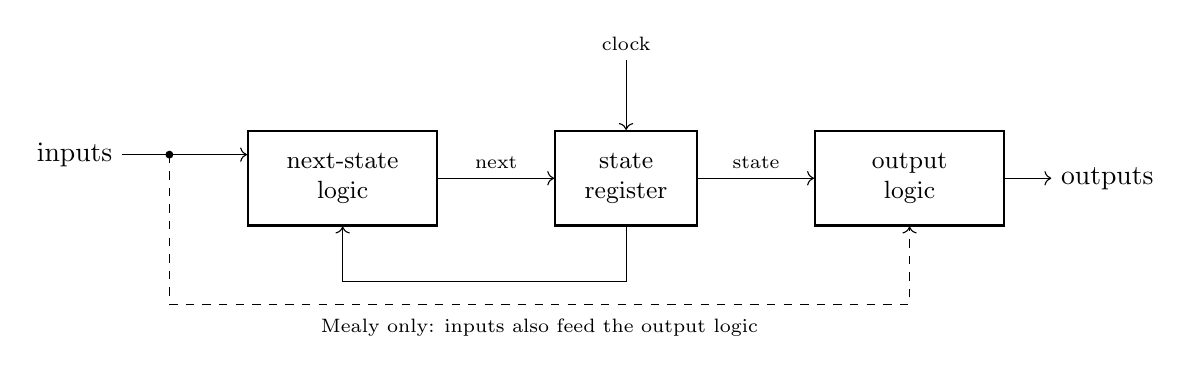
\begin{tikzpicture}[box/.style={draw,thick,minimum height=1.2cm,align=center,font=\small}]
  \node[box,minimum width=2.4cm] (ns) at (0,0) {next-state\\logic};
  \node[box,minimum width=1.8cm] (sr) at (3.6,0) {state\\register};
  \node[box,minimum width=2.4cm] (ol) at (7.2,0) {output\\logic};
  \draw[->] (-2.8,0.3) node[left]{inputs} -- ([yshift=0.3cm]ns.west);
  \draw[->] (ns) -- node[above,font=\scriptsize]{next} (sr);
  \draw[->] (sr) -- node[above,font=\scriptsize]{state} (ol);
  \draw[->] (ol) -- ++(1.8,0) node[right]{outputs};
  \draw[->] (sr.south) -- ++(0,-0.7) -| (ns.south);
  \draw[->] (3.6,1.5) node[above,font=\scriptsize]{clock} -- (sr.north);
  \fill (-2.2,0.3) circle (0.05);
  \draw[->,dashed] (-2.2,0.3) -- (-2.2,-1.6) -- (7.2,-1.6) -- (ol.south);
  \node[font=\scriptsize] at (2.5,-1.9) {Mealy only: inputs also feed the output logic};
\end{tikzpicture}
\caption{Structure of a finite state machine.}
\label{fig:fsmblock}
\end{figure}

\paragraph{Moore versus Mealy.}
\begin{itemize}
  \item In a \term{Moore machine}, the outputs depend only on the current state. Outputs are stable for a whole cycle and glitch-free, but they react to an input one cycle later.
  \item In a \term{Mealy machine}, the outputs depend on the current state \emph{and} the current inputs. Mealy machines react within the same cycle and often need fewer states, but their outputs can glitch when the inputs do.
\end{itemize}

\paragraph{State encoding.} The states must be given binary codes:
\begin{itemize}
  \item \textbf{Binary}: number the states $0, 1, 2, \ldots$. Fewest flip-flops: $\lceil\log_2(\text{number of states})\rceil$.
  \item \textbf{One-hot}: one flip-flop per state, exactly one of them 1. More flip-flops, but the next-state logic is simple and fast. Popular in FPGAs.
  \item \textbf{Gray}: consecutive states differ by one bit, which reduces switching power and glitches.
\end{itemize}

\section{Example: how many flip-flops for a traffic light?}

\begin{worked}{the minimum flip-flops for a traffic-light FSM}
A traffic light stays green for 30\,s, yellow for 5\,s and red for 25\,s, then repeats. The controller's clock has a 1\,s period, and the FSM must count the seconds itself (no separate timer). What is the minimum number of flip-flops?

Every second of the 60-second cycle must be a distinct state, because the machine must know how long it has been in each color. That is $30 + 5 + 25 = 60$ states. Minimum flip-flops: $\lceil \log_2 60 \rceil = 6$ (since $2^5 = 32 < 60 \le 64 = 2^6$).
\end{worked}

A common alternative design uses a 3-state color FSM (2 flip-flops) plus a separate countdown timer big enough for 30 (5 flip-flops): 7 flip-flops in total. It is often cleaner, but it is not the minimum. Read whether the question asks for the minimum.

\begin{onoa}
A reported question asks for the minimum number of flip-flops for a traffic-light FSM, given the green, yellow and red durations and a clock period. The method: total cycles in one full loop $=$ (sum of the durations) / (clock period); minimum flip-flops $= \lceil \log_2(\text{total cycles}) \rceil$.
\end{onoa}

\section{Example: a sequence detector}

A \term{sequence detector} watches a serial input, one bit per clock cycle, and outputs 1 when a particular pattern has just arrived. With \term{overlap}, the end of one match may also be the start of the next.

\begin{worked}{detecting 1011 with overlap (Mealy)}
Each state records how much of the pattern 1011 has been seen so far:
\begin{itemize}
  \item S0: nothing useful yet.
  \item S1: seen ``1''.
  \item S2: seen ``10''.
  \item S3: seen ``101''.
\end{itemize}
The transitions, written as input/output:
\begin{center}
\begin{tabular}{lll}
\toprule
State & Input 0 & Input 1 \\
\midrule
S0 & S0 / 0 & S1 / 0 \\
S1 (``1'') & S2 / 0 & S1 / 0 \quad (``11'': the last 1 may start a match) \\
S2 (``10'') & S0 / 0 \quad (``100'': start over) & S3 / 0 \\
S3 (``101'') & S2 / 0 \quad (``1010'' ends in ``10'') & S1 / \textbf{1} \quad (match; last 1 restarts) \\
\bottomrule
\end{tabular}
\end{center}
The tricky entries are where a mismatch still leaves part of a pattern. From S3 on input 1, the machine has seen 1011: it outputs 1, and the final 1 is the start of a possible new match, so it goes to S1 (that is the overlap). From S3 on input 0, the last two bits ``10'' are a valid start, so it goes to S2, not S0.

Check with the input 1011011: states S0 $\to$ S1 $\to$ S2 $\to$ S3 $\to$ S1 (output 1) $\to$ S2 $\to$ S3 $\to$ S1 (output 1). Two matches, ending at bits 4 and 7, as expected.
\end{worked}

\begin{figure}[h]
\centering
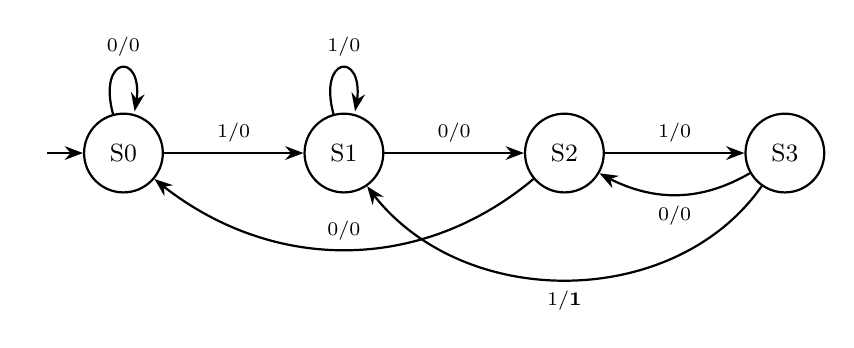
\begin{tikzpicture}[->,>=Stealth,node distance=2.8cm,auto,
    every state/.style={draw,thick,minimum size=1.0cm,font=\small},
    every edge/.style={draw,thick}]
  \node[state,initial,initial text={}] (s0) {S0};
  \node[state] (s1) [right of=s0] {S1};
  \node[state] (s2) [right of=s1] {S2};
  \node[state] (s3) [right of=s2] {S3};
  \path (s0) edge node[font=\scriptsize] {1/0} (s1)
        (s0) edge[loop above] node[font=\scriptsize] {0/0} ()
        (s1) edge node[font=\scriptsize] {0/0} (s2)
        (s1) edge[loop above] node[font=\scriptsize] {1/0} ()
        (s2) edge node[font=\scriptsize] {1/0} (s3)
        (s2) edge[bend left=40] node[font=\scriptsize,above] {0/0} (s0)
        (s3) edge[bend left=30] node[font=\scriptsize,below] {0/0} (s2)
        (s3) edge[bend left=55] node[font=\scriptsize,below] {1/\textbf{1}} (s1);
\end{tikzpicture}
\caption{Mealy state diagram for detecting 1011 with overlap. Labels are input/output.}
\label{fig:seq1011}
\end{figure}

A \textbf{Moore} version needs one more state, S4 (``just matched''), whose output is 1. From S4, input 1 goes to S1 and input 0 goes to S2 (since ``10110'' ends in ``10''). Moore machines typically need more states than Mealy machines for the same job, because the output must be attached to a state.

\paragraph{The general recipe for sequence detectors.} For a pattern of length $L$, the Mealy machine has $L$ states (one per prefix length, $0$ to $L-1$). For each state and input, the next state is the longest suffix of (seen-so-far + new bit) that is also a prefix of the pattern. Doing this carefully is what makes overlapping detection correct.

\section{Other useful counters}

\begin{itemize}
  \item \term{Ring counter}: a shift register with the last output fed back to the first, holding a single 1. With $N$ flip-flops it has $N$ states (one-hot).
  \item \term{Johnson counter}: a shift register with the \emph{inverted} last output fed back. With $N$ flip-flops it cycles through $2N$ states, and only one bit changes per step.
  \item \term{Linear-feedback shift register} (LFSR): a shift register whose input is the XOR of certain bits. With the right taps, $N$ flip-flops step through all $2^N - 1$ nonzero states in a pseudo-random order. LFSRs generate test patterns, scramble data and compute checksums (CRCs).
  \item \term{Gray-code counter}: counts in Gray code, so only one bit changes per step; used for pointers that cross clock domains (Chapter~\ref{ch:rtl}).
\end{itemize}

\section{Summary}

\begin{itemize}
  \item A binary counter's bit $k$ runs at $f_{clk}/2^{k+1}$; the MSB of $n$ bits has period $2^n T_{clk}$.
  \item A mod-$N$ counter needs $\lceil\log_2 N\rceil$ flip-flops.
  \item Divide by 2: toggle flip-flop. Divide by $2^n$: $n$ stages. Even $N$: toggle every $N/2$ cycles.
  \item Odd $N$ with 50\% duty: a rising-edge signal high for $(N-1)/2$ cycles, ORed with a copy delayed half a cycle by a falling-edge flip-flop.
  \item Divide by 2 with 25\% duty: $Q \cdot \nt{CLK}$ (glitch-free).
  \item FSM: state register + next-state logic + output logic. Moore outputs depend on state only; Mealy on state and inputs.
  \item Minimum flip-flops $= \lceil\log_2(\text{states})\rceil$; one-hot uses one per state.
  \item Overlapping sequence detectors: after a match or mismatch, go to the state of the longest suffix that is still a prefix.
\end{itemize}

\section{Exercises}

\begin{enumerate}
  \item A 3-bit ripple counter is clocked at 16\,MHz. What is the frequency of its most significant bit?
  \item How many flip-flops are needed for a mod-10 counter? A mod-100 counter?
  \item Design a divide-by-4 from a 100\,MHz clock. What is the output frequency and how many flip-flops are needed?
  \item Describe a divide-by-6 circuit with a 50\% duty cycle.
  \item Describe a divide-by-5 circuit with a 50\% duty cycle.
  \item An FSM has 12 states. How many flip-flops does it need with binary encoding? With one-hot encoding?
  \item What is the difference between a Moore and a Mealy machine? Which usually needs more states?
  \item How many states does a Mealy machine need to detect the overlapping sequence 110?
  \item A traffic light is green for 20\,s, yellow for 4\,s and red for 24\,s, with a 2\,s clock period. What is the minimum number of flip-flops?
  \item Why is $Q \cdot \nt{CLK}$ preferred over $Q \cdot CLK$ for a 25\% duty-cycle divide-by-2?
  \item How many states does a 4-flip-flop Johnson counter have? A 4-flip-flop maximal LFSR?
\end{enumerate}

\subsection*{Answers}
\begin{enumerate}
  \item $16/2^3 = 2$\,MHz.
  \item 4 ($2^4 = 16 \ge 10$). 7 ($2^7 = 128 \ge 100$).
  \item Two toggle stages: 25\,MHz, 2 flip-flops.
  \item A mod-3 counter on the rising edge; toggle the output each time the counter wraps (every 3 cycles). High for 3 cycles, low for 3.
  \item A mod-5 counter on the rising edge; make $P$ high for 2 of the 5 states; delay $P$ by half a cycle with a falling-edge flip-flop to get $N$; output $P$ OR $N$, which is high for 2.5 of every 5 cycles.
  \item Binary: 4 ($2^4 = 16 \ge 12$). One-hot: 12.
  \item Moore outputs depend only on the state; Mealy outputs depend on the state and the current inputs. Moore usually needs more states.
  \item 3 (prefixes of length 0, 1 and 2).
  \item $(20 + 4 + 24)/2 = 24$ cycles, so $\lceil\log_2 24\rceil = 5$.
  \item $Q$ changes $t_{cq}$ after each rising edge. With $Q \cdot CLK$, when $Q$ falls the clock has already risen, giving a short glitch. With $\nt{CLK}$, that input has already fallen before $Q$ changes, so the AND output stays low.
  \item Johnson: $2 \times 4 = 8$ states. LFSR: $2^4 - 1 = 15$ states.
\end{enumerate}


\part{Speed, Power and the Real World}
\chapter{Delay: Why Circuits Take Time}
\label{ch:delay}

Chapter~\ref{ch:timing} used gate delays as given numbers. This chapter explains where they come from and how designers control them. One idea runs through all of it: a transistor behaves like a resistor, whatever it drives behaves like a capacitor, and delay is the time to charge that capacitor through that resistor.

\section{The RC model of a gate}

When a gate's output switches from 0 to 1, its PMOS pull-up network charges the output node from 0 to $\VDD$. Everything connected to that node is capacitance (Chapter~\ref{ch:capind}):
\begin{itemize}
  \item the input (gate) capacitance of every gate it drives, called its \term{fan-out};
  \item the capacitance of the wire;
  \item the gate's own drain (diffusion) capacitance, its \term{parasitic} capacitance.
\end{itemize}
The pull-up network acts like a resistor, $R$, so the output rises like an RC charging curve. It reaches 50\% after about $0.69\,RC$ (Section~\ref{sec:rc}):
\[
  \boxed{t_{pd} \approx 0.69\,R\,C_{load}}
\]
The same applies to a falling output through the pull-down network.

\begin{worked}{an inverter driving four others}
A unit inverter has an effective resistance of 10\,k$\Omega$, an input capacitance of 1\,fF and a parasitic output capacitance of 1\,fF. It drives four identical inverters (a \term{fan-out of 4}).

$C_{load} = 4 \times 1 + 1 = 5$\,fF. Delay $\approx 0.69 \times 10^4 \times 5\times10^{-15} \approx 35$\,ps.
\end{worked}

The delay of an inverter driving four copies of itself, the \term{FO4 delay}, is a standard yardstick for how fast a manufacturing process is. Designers often describe a clock period as ``so many FO4 delays,'' which stays meaningful across processes.

\section{Rise, fall and propagation}

Precise definitions, all measured on waveforms:
\begin{itemize}
  \item $t_{pLH}$, $t_{pHL}$: from the input crossing 50\% to the output crossing 50\%, for a rising or falling output. The propagation delay is often quoted as their average.
  \item \term{Rise time} and \term{fall time}: how long the output takes to go from 10\% to 90\% of its swing (or the reverse). For an RC curve that is $2.2\,RC$.
  \item The \term{slew} or transition time of a signal is its rise or fall time. A slowly rising input makes the next gate slower and wastes power, because both of its transistors are partly on for longer.
\end{itemize}

\section{How sizing changes delay}

From Chapter~\ref{ch:mosfet}, a transistor's current is proportional to its width $W$, so its resistance is proportional to $1/W$. Its gate capacitance is proportional to $W$. That gives the basic tension of sizing:

\begin{bigidea}
Making a gate $k$ times wider makes it $k$ times stronger (its own delay falls), but it presents $k$ times more input capacitance to whatever drives it (the previous gate's delay rises). Making gates bigger is not free speed; it moves delay backward.
\end{bigidea}

\section{Driving a big load: buffer chains}

Suppose a small gate must drive a huge capacitance: a long bus, a clock net, an output pin. Driving it directly is very slow, and making the small gate huge just loads \emph{its} driver. The solution is a chain of inverters, each bigger than the last by a constant factor, a \term{tapered buffer}.

If the load is $F$ times the input capacitance of the first inverter and you use $N$ stages, each stage should be $F^{1/N}$ times bigger than the one before. Analysis (and practice) shows the best ratio per stage is around \textbf{4}, so
\[
  N \approx \log_4 F.
\]

\begin{worked}{sizing a buffer chain}
A unit inverter must drive a load 1024 times its own input capacitance. With a ratio of 4 per stage: $\log_4 1024 = 5$ stages, sized 1, 4, 16, 64 and 256, with the last one driving the 1024 load. Each stage sees a fan-out of 4, so each has roughly an FO4 delay, and the total is about 5 FO4.
\end{worked}

\section{Logical effort}
\label{sec:logeffort}

\term{Logical effort} is a method for estimating and optimizing the delay of a path of different gates. It writes the delay of each gate, in units of a basic inverter delay, as
\[
  d = g\,h + p
\]
\begin{itemize}
  \item $g$, the \term{logical effort}: how much worse the gate is at driving current than an inverter with the same input capacitance. It depends only on the gate type.
  \item $h$, the \term{electrical effort} or fan-out: $C_{out}/C_{in}$.
  \item $p$, the \term{parasitic delay}: the gate's delay from its own internal capacitance.
\end{itemize}

\begin{center}
\begin{tabular}{lcc}
\toprule
Gate & Logical effort $g$ & Parasitic delay $p$ \\
\midrule
Inverter & 1 & 1 \\
NAND2 & 4/3 & 2 \\
NAND3 & 5/3 & 3 \\
NOR2 & 5/3 & 2 \\
NOR3 & 7/3 & 3 \\
\bottomrule
\end{tabular}
\end{center}
(These values assume a PMOS twice as wide as an NMOS for equal strength.) NOR has a higher logical effort than NAND, which is the quantitative version of ``NAND is better than NOR'' (Chapter~\ref{ch:cmos}).

For a path of $N$ gates, multiply the logical efforts into $G$, take the overall electrical effort $H = C_{out,\text{path}}/C_{in,\text{path}}$, and form the \term{path effort} $F = G\,H$ (ignoring branching). The fastest design gives every stage the same effort, $f = F^{1/N}$, and the minimum delay is
\[
  D = N\,F^{1/N} + P,
\]
where $P$ is the sum of the parasitic delays.

\begin{worked}{a three-gate path}
A path is inverter, NAND2, inverter. The final load is 48 times the first inverter's input capacitance ($H = 48$).

$G = 1 \times \tfrac43 \times 1 = \tfrac43$. $F = GH = \tfrac43 \times 48 = 64$. Best stage effort $f = 64^{1/3} = 4$. $P = 1 + 2 + 1 = 4$. Minimum delay $D = 3 \times 4 + 4 = 16$ inverter delay units. Each stage is then sized so that its $g\,h = 4$.
\end{worked}

\section{Elmore delay: delays through networks}

Often a driver charges several capacitances through a chain or tree of resistances (a wire with many segments, or a stack of transistors). The \term{Elmore delay} is a simple estimate of the time constant to a given node:

\begin{bigidea}
Elmore delay: for each resistor on the path from the source to the node of interest, multiply its resistance by \emph{all} the capacitance downstream of it, then add up the products:
\[
  \tau_{Elmore} = \sum_i R_i \cdot C_{\text{downstream of } R_i}.
\]
\end{bigidea}

\begin{figure}[h]
\centering
\begin{circuitikz}
  \draw (0,0) node[left]{driver} to[R, l=$R_1$, o-] (2,0) to[R, l=$R_2$] (4,0) to[R, l=$R_3$] (6,0) node[right]{end};
  \draw (2,0) to[C, l=$C_1$, *-] (2,-1.5) node[ground]{};
  \draw (4,0) to[C, l=$C_2$, *-] (4,-1.5) node[ground]{};
  \draw (6,0) to[C, l=$C_3$, *-] (6,-1.5) node[ground]{};
\end{circuitikz}
\caption{An RC ladder, the model of a wire divided into three segments.}
\label{fig:ladder}
\end{figure}

\begin{worked}{Elmore delay of a ladder}
In Figure~\ref{fig:ladder}, every $R$ and every $C$ is equal. To the end node:
\[
  \tau = R_1(C_1 + C_2 + C_3) + R_2(C_2 + C_3) + R_3 C_3 = 3RC + 2RC + RC = 6RC.
\]
With $R = 100~\Omega$ and $C = 10$\,fF, $\tau = 6 \times 10^{-12} = 6$\,ps.
\end{worked}

\section{Wires}

A wire's resistance and capacitance are both spread along its length. Split a wire of length $L$ into $n$ segments, and the Elmore delay grows like $1 + 2 + \cdots + n \approx n^2/2$. Since both $R$ and $C$ are proportional to $L$:
\[
  t_{wire} \propto R_{wire}\,C_{wire} \propto L^2.
\]
(For a uniformly distributed RC wire, the 50\% delay is about $0.38\,R_{wire}C_{wire}$.)

\begin{bigidea}
An unbuffered wire's delay grows with the \emph{square} of its length. Doubling the length quadruples the delay. The fix is to break a long wire into segments with \term{repeaters} (buffers) between them: each short segment has a small delay, and the total grows only linearly with length.
\end{bigidea}

\begin{worked}{repeaters}
An unbuffered wire has a delay of 400\,ps. Insert one repeater in the middle. Each half has a quarter of the original delay (half the length, squared): 100\,ps each, 200\,ps for both, plus the repeater's own delay (say 20\,ps): 220\,ps total, almost half. More repeaters help further, up to the point where the repeaters' own delays dominate.
\end{worked}

As transistors have shrunk, they have become much faster, but thin wires have become \emph{more} resistive. In modern chips, long-wire delay often matters more than gate delay, which is why chip architects work hard to keep communicating blocks close together.

\section{Other effects on delay}

\begin{itemize}
  \item \textbf{Supply voltage.} A gate's delay is roughly $C\,\VDD/I$, and drive current grows with $(\VDD - \Vt)$ raised to a power between 1 and 2. Raising $\VDD$ speeds gates up; lowering it slows them, dramatically so as $\VDD$ approaches $\Vt$.
  \item \textbf{Temperature and process.} Hot transistors are usually slower (lower mobility), and manufacturing variation makes some chips faster than others (Chapter~\ref{ch:pvt}).
  \item \textbf{Input ordering in stacks.} In a series stack, the transistor nearest the output must discharge the most internal capacitance. Connecting the \emph{latest-arriving} input to the transistor nearest the output makes the gate respond fastest to it, because the other transistors have already turned on and discharged the internal nodes.
  \item \textbf{Miller effect.} Capacitance between a gate's input and output appears doubled when they swing in opposite directions (as they do in an inverter), adding delay. The same effect makes coupling between neighboring wires worse when they switch in opposite directions (Chapter~\ref{ch:wires}).
\end{itemize}

\section{Summary}

\begin{itemize}
  \item Gate delay $\approx 0.69\,R\,C_{load}$; the load is fan-out input capacitance plus wire plus parasitic capacitance.
  \item FO4 delay is the standard yardstick for process speed.
  \item Wider gates are stronger but load their drivers more.
  \item Drive big loads with a tapered chain, about 4 times larger per stage: $N \approx \log_4(C_{load}/C_{in})$.
  \item Logical effort: $d = gh + p$; NAND2 has $g = 4/3$, NOR2 $5/3$. Best path delay $D = NF^{1/N} + P$.
  \item Elmore delay: sum of each resistance times all downstream capacitance.
  \item Unbuffered wire delay grows with $L^2$; repeaters make it linear.
  \item Higher $\VDD$ is faster; put the latest-arriving input nearest the output.
\end{itemize}

\section{Exercises}

\begin{enumerate}
  \item A gate with a 5\,k$\Omega$ effective resistance drives 20\,fF. Estimate its delay.
  \item A gate's fan-out doubles. Roughly what happens to its delay, assuming the fan-out capacitance dominates?
  \item A unit inverter must drive 64 times its input capacitance. How many stages should a tapered buffer chain have, and what sizes?
  \item What are the logical efforts of an inverter, a NAND2 and a NOR2? Why is the NOR2's larger?
  \item An RC ladder has $R_1 = R_2 = 1$\,k$\Omega$ and $C_1 = C_2 = 10$\,fF (the same shape as Figure~\ref{fig:ladder} with two segments). Find the Elmore delay to the end.
  \item An unbuffered wire's length triples. By what factor does its delay change?
  \item Why should the latest-arriving input of a NAND gate drive the transistor nearest the output?
  \item Does raising the supply voltage make a gate faster or slower? Why?
\end{enumerate}

\subsection*{Answers}
\begin{enumerate}
  \item $0.69 \times 5000 \times 20\times10^{-15} \approx 69$\,ps.
  \item It roughly doubles.
  \item $\log_4 64 = 3$ stages, sized 1, 4 and 16 (the last drives the 64 load).
  \item 1, 4/3 and 5/3. NOR2 has two PMOS in series; to match an inverter's strength they must be very wide, giving more input capacitance for the same drive.
  \item $R_1(C_1 + C_2) + R_2 C_2 = 1000 \times 20\times10^{-15} + 1000 \times 10\times10^{-15} = 30$\,ps.
  \item $3^2 = 9$ times.
  \item By the time the last input arrives, the other transistors are already on and the internal nodes have been discharged, so only the transistor nearest the output has to switch, and the output responds fastest.
  \item Faster: more voltage gives more drive current (more overdrive above $\Vt$), so capacitances charge and discharge more quickly. The cost is more power.
\end{enumerate}

\chapter{Power: Where the Energy Goes}
\label{ch:power}

Power limits modern chips more than anything else. A GPU could be faster if it could burn more power, but it would melt (Chapter~\ref{ch:heat}), and a phone could be faster but its battery would die. This chapter explains exactly where a chip's power goes, derives the formula behind the assessment question ``if frequency and voltage double, what happens to dynamic power?'', and surveys the techniques engineers use to save power.

\section{Three kinds of power}

\begin{enumerate}
  \item \term{Dynamic power}: spent charging and discharging capacitance every time a signal switches. Usually the largest part when a chip is busy.
  \item \term{Short-circuit power}: during each transition, both the pull-up and pull-down are briefly on together, and current flows straight from the supply to ground.
  \item \term{Leakage power} (static power): transistors that are ``off'' still leak a little current, all the time, even when nothing switches.
\end{enumerate}

\section{Dynamic power}

Consider an inverter driving a load capacitance $C$ (Figure~\ref{fig:dynpower}).

\begin{figure}[h]
\centering
\begin{circuitikz}
  \draw (0,0) node[pmos](p){} (0,-2.2) node[nmos](n){};
  \draw (p.S) node[vdd]{$\VDD$};
  \draw (n.S) node[ground]{};
  \draw (p.D) -- (n.D);
  \draw (p.G) -- (n.G);
  \draw ($(p.G)!0.5!(n.G)$) to[short,-o] ++(-0.8,0) node[left]{In};
  \draw ($(p.D)!0.5!(n.D)$) to[short,*-] ++(1.6,0) coordinate(o) to[C, l=$C$] ++(0,-1.6) node[ground]{};
  \draw[->,red!70!black,thick] (0.45,0.2) .. controls (1.2,0.2) .. (1.55,-0.8);
  \node[red!70!black,font=\small,right] at (1.5,0.3) {charge: $CV^2$ from supply};
  \draw[->,blue!70!black,thick] (1.55,-1.5) .. controls (1.0,-2.6) .. (0.45,-2.4);
  \node[blue!70!black,font=\small,right] at (1.6,-2.6) {discharge to ground};
\end{circuitikz}
\caption{Each 0-to-1 output transition draws charge from the supply; each 1-to-0 transition dumps it to ground.}
\label{fig:dynpower}
\end{figure}

\paragraph{Charging (output 0 $\to$ 1).} The PMOS connects the capacitor to $\VDD$. Charge $Q = C\VDD$ flows out of the supply at voltage $\VDD$, so the supply delivers energy $Q\VDD = C\VDD^2$. Of that, $\tfrac12 C\VDD^2$ ends up stored in the capacitor (Chapter~\ref{ch:capind}); the other half is turned into heat in the PMOS's resistance.

\paragraph{Discharging (output 1 $\to$ 0).} The NMOS connects the capacitor to ground, and the stored $\tfrac12 C\VDD^2$ is turned into heat in the NMOS.

So every full cycle of charge and discharge consumes $C\VDD^2$ from the supply. If the node does this $f$ times per second, the power is $C\VDD^2 f$. Most nodes do not switch every cycle, so we multiply by an \term{activity factor} $\alpha$: the fraction of clock cycles in which the node makes a 0-to-1 transition.

\begin{center}
\fbox{\parbox{0.6\linewidth}{\centering\vspace{0.2em}
$\displaystyle P_{dynamic} = \alpha\, C\, \VDD^2\, f$\vspace{0.4em}}}
\end{center}

\begin{itemize}
  \item $\alpha$: activity factor. A clock rises once every cycle, so $\alpha = 1$. Typical data nodes have $\alpha$ around 0.1 to 0.25.
  \item $C$: the total capacitance that switches.
  \item $\VDD$: supply voltage, and it is \emph{squared}.
  \item $f$: clock frequency.
\end{itemize}

\begin{bigidea}
Dynamic power is proportional to the \emph{square} of the voltage and only linearly to frequency and capacitance. Lowering the voltage is the most powerful way to save power.
\end{bigidea}

\begin{worked}{a chip's dynamic power}
A block has 1\,nF of total switching capacitance, an average activity factor of 0.2, a 1.0\,V supply and a 1\,GHz clock.
\[
  P = 0.2 \times 10^{-9} \times 1.0^2 \times 10^9 = 0.2~\text{W}.
\]
\end{worked}

\section{Scaling questions}
\label{sec:powerscaling}

Assessment questions change one or more of the variables and ask for the new power. Since $P \propto \alpha C V^2 f$, multiply the factors, remembering to square the voltage factor.

\begin{center}
\begin{tabular}{lll}
\toprule
Change & New dynamic power & Working \\
\midrule
$f \times 2$ & $\times 2$ & linear in $f$ \\
$V \times 2$ & $\times 4$ & $2^2$ \\
$f \times 2$ \textbf{and} $V \times 2$ & $\times 8$ & $2 \times 2^2$ \\
$V \times 0.5$ & $\times 0.25$ & $0.5^2$ \\
$V$ up 10\%, $f$ up 20\% & $\times 1.452$ (+45\%) & $1.1^2 \times 1.2$ \\
$(f, 2V) \to (4f, 3V)$ & $\times 9$ & $4 \times (3/2)^2$ \\
$V \times 0.9$, $f \times 0.9$ & $\times 0.729$ & $0.9^2 \times 0.9$ \\
$C \times 2$ (twice the logic) & $\times 2$ & linear in $C$ \\
\bottomrule
\end{tabular}
\end{center}

\begin{onoa}
``If the clock frequency doubles and the supply voltage doubles, what is the dynamic power?'' was an Ignite assessment question. Answer: \textbf{8 times} the original ($2$ for frequency times $2^2 = 4$ for voltage). Reported variants include voltage up 10\% with frequency up 20\% ($\times 1.45$) and a change from $(f, 2V)$ to $(4f, 3V)$ ($\times 9$; note that the voltage factor is $3V/2V = 1.5$, squared to 2.25).
\end{onoa}

\begin{trap}
Watch for the starting point. In ``$(f, 2V) \to (4f, 3V)$'' the voltage does not triple; it goes from $2V$ to $3V$, a factor of 1.5. Always divide new by old for each variable before multiplying.
\end{trap}

\section{Power versus energy}

\term{Power} is energy per second. \term{Energy} is what drains a battery. The energy for one operation is
\[
  E_{op} = \alpha C \VDD^2,
\]
with no $f$ in it. So:
\begin{itemize}
  \item Running the same work at double the frequency (same voltage) \emph{doubles the power} but uses \emph{the same energy} per operation; the work just finishes sooner.
  \item Lowering the voltage reduces \emph{both} power and energy per operation.
\end{itemize}
This is why ``slow down to save energy'' only works if the voltage comes down too.

\section{Short-circuit power}

During an input transition, there is a moment when the input is between $\Vtn$ and $\VDD - |\Vtp|$ and both transistors are on. Current flows straight from $\VDD$ to ground. The slower the input transition, the longer this lasts, which is one reason designers keep signal transitions sharp. In a well-designed chip, short-circuit power is usually 10\% or less of dynamic power.

\section{Leakage power}
\label{sec:leakage}

Even with no switching at all, current trickles through transistors that are supposed to be off. Leakage power is $P_{leak} = I_{leak}\,\VDD$. The main sources:

\begin{itemize}
  \item \textbf{Subthreshold leakage}: an ``off'' transistor still conducts a little, and this current grows \emph{exponentially} as $\Vt$ decreases (Chapter~\ref{ch:mosfet}) and as temperature increases (Chapter~\ref{ch:semis}). It is usually the largest leakage source.
  \item \textbf{Gate leakage}: electrons tunnel through extremely thin gate oxide. High-$k$ gate materials were introduced largely to reduce it.
  \item \textbf{Junction leakage}: small reverse current through the source/drain diodes.
\end{itemize}

Two transistors that are both off and in series leak much less than one (the \term{stack effect}), because the node between them rises slightly and turns both off more firmly.

As transistors shrank, thresholds had to fall to keep them fast, and leakage grew from negligible to a large fraction of total power. Leakage also feeds on heat: a hotter chip leaks more and gets hotter still (Chapter~\ref{ch:heat}).

\section{Saving power}

\begin{center}
\begin{tabularx}{\linewidth}{>{\raggedright\arraybackslash}p{3.3cm}>{\raggedright\arraybackslash}p{2.3cm}>{\raggedright\arraybackslash}X}
\toprule
Technique & Reduces & How \\
\midrule
Clock gating & dynamic & Stop the clock to idle registers. The clock network has $\alpha = 1$ and is a big part of dynamic power, so this is the most common technique. \\
Power gating & leakage (and dynamic) & Cut off the supply to an idle block with a large ``sleep'' transistor (a header PMOS or footer NMOS). \\
DVFS & dynamic and leakage & Dynamic voltage and frequency scaling: lower $V$ and $f$ together when full speed is not needed. \\
Multi-$\Vt$ cells & leakage & High-$\Vt$ (low-leakage) transistors on paths that are not timing-critical. \\
Multiple voltage domains & dynamic & Run slower blocks at a lower $\VDD$; level shifters translate signals between domains. \\
Body biasing & leakage or delay & Reverse body bias raises $\Vt$ (less leakage); forward bias lowers it (faster). \\
Reducing activity & dynamic & Avoid useless toggling: operand isolation, Gray-coded counters, removing glitches. \\
Parallelism & dynamic & Two slower units at a lower voltage can beat one fast unit (below). \\
\bottomrule
\end{tabularx}
\end{center}

\paragraph{Clock gating done safely.} Simply ANDing a clock with an enable signal can produce glitches if the enable changes while the clock is high. The standard \term{integrated clock gating} (ICG) cell captures the enable in a latch that is transparent only while the clock is low, then ANDs the latched enable with the clock. The enable can only change while the clock is low, so the gated clock is always clean.

\paragraph{Power gating trade-offs.} A power-gated block loses its state, so registers that must survive need special \term{retention} flip-flops (or the state is saved elsewhere). Outputs of a powered-off block float, so \term{isolation cells} clamp them to safe values. Waking up takes time and causes a surge of current as the block's capacitance recharges.

\begin{worked}{parallelism saves power}
One processing unit runs at frequency $f$ and voltage $V$. Replace it with two identical units, each running at $f/2$ (same total throughput), which lets the voltage drop to $0.7V$. Ignoring overhead, the capacitance doubles:
\[
  \frac{P_{new}}{P_{old}} = \frac{2C \times (0.7V)^2 \times f/2}{C V^2 f} = 0.49.
\]
Same work, about half the power. This is a big part of why GPUs, with thousands of moderately clocked cores, are so energy efficient for parallel work.
\end{worked}

\begin{worked}{how much power is left after power gating?}
In an idle mode, a design power-gates most of its logic. The numbers (with assumptions stated):
\begin{itemize}
  \item Standard cells: 40\,W dynamic and 10\,W leakage when active. 10\% of the cells must stay on (always-on logic); the other 90\% are gated with 80\% efficiency (gating removes 80\% of their leakage).
  \item RAMs: 20\,W dynamic and 6\,W leakage. All are gated with 90\% efficiency.
  \item Gated blocks do no switching, so their dynamic power becomes zero; the always-on cells keep their share of dynamic power.
\end{itemize}
Standard-cell leakage left: $10 \times [0.1 + 0.9 \times (1 - 0.8)] = 10 \times 0.28 = 2.8$\,W.
RAM leakage left: $6 \times (1 - 0.9) = 0.6$\,W.
Dynamic left: $0.1 \times 40 = 4$\,W from the always-on cells; RAMs 0\,W.
Total in idle: $2.8 + 0.6 + 4 = 7.4$\,W, down from 76\,W.
\end{worked}

\begin{onoa}
A reported question gives power-gating efficiencies for standard cells (80\%) and RAMs (90\%), with 10\% of cells always on, and asks for the remaining dynamic and leakage power. The exact answer depends on the numbers given, but the method is the one above: split each block into always-on and gated parts, remove the stated fraction of leakage from the gated part, and remove the gated part's dynamic power.
\end{onoa}

\section{The bigger picture: Dennard scaling and dark silicon}

For decades, shrinking transistors brought a free lunch called \term{Dennard scaling}: smaller transistors could run at lower voltage, so power per unit area stayed constant while chips got faster. Around 2005 this broke down. Voltage could no longer drop much, because lower thresholds would make leakage explode. Power density started rising with each generation, clock frequencies stopped climbing (most processors have stayed around 3 to 5\,GHz since), and the industry turned to parallelism: multiple cores, and massively parallel GPUs.

Today a chip often cannot run all of its transistors at full speed at once without exceeding its power and cooling budget; some must be idle or slowed at any moment. This is called \term{dark silicon}. A chip's \term{thermal design power} (TDP) is the sustained power its cooling system is designed to remove.

\section{Summary}

\begin{itemize}
  \item Dynamic power $= \alpha C \VDD^2 f$: each charge-discharge cycle costs $C\VDD^2$; half is lost charging and half discharging.
  \item Scaling: multiply the factor changes, squaring the voltage factor. $f\times2$ and $V\times2$ gives $\times8$.
  \item Energy per operation $= \alpha C \VDD^2$, independent of $f$. Only lowering voltage saves energy per operation.
  \item Short-circuit power comes from both transistors being on during transitions; sharp edges minimize it.
  \item Leakage grows exponentially as $\Vt$ falls and temperature rises.
  \item Clock gating cuts dynamic power; power gating cuts leakage; DVFS cuts both.
  \item Parallel units at lower voltage can do the same work for less power.
  \item The end of Dennard scaling ended rising clock speeds and pushed the industry toward parallelism.
\end{itemize}

\section{Exercises}

\begin{enumerate}
  \item A block has $\alpha = 0.2$, $C = 1$\,nF, $\VDD = 1.0$\,V and $f = 1$\,GHz. Find its dynamic power.
  \item Clock frequency and supply voltage both double. By what factor does dynamic power change?
  \item Supply voltage rises 10\% and frequency rises 20\%. What is the percentage change in dynamic power?
  \item A chip moves from frequency $f$ at voltage $2V$ to frequency $4f$ at voltage $3V$. By what factor does dynamic power change?
  \item Voltage and frequency are both reduced by 10\%. What fraction of the original dynamic power remains?
  \item A processor runs the same program twice as fast at the same voltage. What happens to its power, and to the energy the program uses?
  \item Which kind of power does clock gating reduce? Which does power gating reduce?
  \item Does leakage power rise or fall with temperature?
  \item What is the activity factor of a clock net?
  \item Compare one core at frequency $f$ and 1.0\,V with two cores at $f/2$ and 0.6\,V each. What is the power ratio, ignoring overhead?
  \item Why can't a designer simply AND a clock with an enable signal to gate it?
\end{enumerate}

\subsection*{Answers}
\begin{enumerate}
  \item $0.2 \times 10^{-9} \times 1 \times 10^9 = 0.2$\,W.
  \item $2 \times 2^2 = 8$.
  \item $1.1^2 \times 1.2 = 1.452$, an increase of about 45\%.
  \item $4 \times (3/2)^2 = 9$.
  \item $0.9^2 \times 0.9 = 0.729$, about 73\%.
  \item Power doubles; energy for the program stays the same (energy per operation does not depend on frequency).
  \item Clock gating: dynamic power. Power gating: leakage power (and the gated block's dynamic power).
  \item Rise (exponentially).
  \item 1.
  \item $2 \times 0.6^2 \times 0.5 = 0.36$: about 36\% of the original power.
  \item If the enable changes while the clock is high, the AND output can produce a shortened pulse or glitch, which flip-flops would treat as a clock edge. A latch-based clock-gating cell allows the enable to change only while the clock is low.
\end{enumerate}

\chapter{Process, Voltage and Temperature}
\label{ch:pvt}

No two chips are identical, and no chip runs in identical conditions all its life. Transistors come out of the factory a little faster or slower; the supply voltage sags under load; the temperature swings from a cold start to full load. A design must work across all of it. Engineers summarize these three sources of variation as \term{PVT}: process, voltage and temperature. This chapter explains each, finishes the temperature question from the assessment, and shows how designers decide which conditions to check.

\section{Process variation}

Manufacturing a chip involves printing features tens of nanometers wide and implanting dopant atoms by the thousands (Chapter~\ref{ch:fab}). Nothing can be done perfectly at that scale, so transistor properties vary:
\begin{itemize}
  \item \textbf{Global variation}: whole wafers or whole chips come out faster or slower than average (for example, a slightly thinner gate oxide everywhere on one wafer).
  \item \textbf{Local variation}: neighboring transistors on the same chip differ. With only a few dozen dopant atoms in a tiny transistor's channel, the random count alone changes its threshold voltage (\term{random dopant fluctuation}). The roughness of printed edges changes channel lengths.
\end{itemize}

Designers describe global variation with \term{process corners}, named by the speed of the NMOS and PMOS transistors:
\begin{center}
\begin{tabular}{ll}
\toprule
Corner & Meaning \\
\midrule
TT & typical NMOS, typical PMOS \\
FF & fast NMOS, fast PMOS \\
SS & slow NMOS, slow PMOS \\
FS & fast NMOS, slow PMOS \\
SF & slow NMOS, fast PMOS \\
\bottomrule
\end{tabular}
\end{center}
The skewed corners (FS and SF) matter for circuits that depend on a balance between pull-up and pull-down, such as an inverter's switching threshold or an SRAM cell's stability (Chapter~\ref{ch:memory}). Local variation is handled statistically, with \term{Monte Carlo} simulation (running many simulations with randomly varied transistors) and with timing margins called on-chip variation (OCV) derates.

A practical consequence is \term{binning}: chips from the same wafer are tested and sorted by how fast they run, and faster chips are sold as higher-end products.

\section{Voltage variation}

The supply voltage a transistor actually sees is lower than the regulator's output and changes over time (Chapters~\ref{ch:electricity} and~\ref{ch:capind}):
\begin{itemize}
  \item \textbf{Regulator tolerance}: the supply is specified as, say, $0.80\,\text{V} \pm 3\%$.
  \item \textbf{Static IR drop}: steady current through the resistance of the power grid lowers the voltage, more so far from the power pins.
  \item \textbf{Dynamic droop}: sudden increases in current cause $L\,di/dt$ dips until decoupling capacitors and the regulator respond.
\end{itemize}
Lower voltage means less overdrive, so transistors are slower. Power-delivery design aims to keep the total drop within a budget, often a few percent.

\section{Temperature}

Chips must work across a wide range of temperatures, from a cold start in an unheated room (or a car in winter) to full load under a heat sink. Typical junction-temperature ranges are about 0 to 100\,\textdegree C for consumer products, and $-40$ to 125\,\textdegree C or more for automotive parts. Temperature changes several things at once:

\begin{center}
\begin{tabular}{lll}
\toprule
Quantity & As temperature rises & Effect \\
\midrule
Carrier mobility $\mu$ & decreases & transistors slower \\
Threshold voltage $\Vt$ & decreases & transistors faster \\
Metal wire resistance & increases & wires slower \\
Subthreshold leakage & increases exponentially & more power, more heat \\
Electromigration & accelerates & shorter wire lifetime \\
\bottomrule
\end{tabular}
\end{center}

\subsection*{Why each happens}

\paragraph{Mobility falls.} Hot atoms vibrate more, so carriers collide with them more often (phonon scattering) and drift more slowly in the same electric field (Section~\ref{sec:tempmobility}).

\paragraph{Wire resistance rises.} Metal electrons are scattered by the same vibrations. Copper's resistance increases by about 0.39\% per \textdegree C.

\paragraph{Threshold voltage falls.} Heat gives carriers more energy, so a smaller gate voltage is enough to form the channel. A typical rate is on the order of 1\,mV per \textdegree C.

\begin{onoa}
The assessment asked how CMOS carrier mobility and wire resistance change as temperature increases. \textbf{Mobility decreases} and \textbf{wire resistance increases}; both make the circuit slower when hot. A complete answer also knows the exception below.
\end{onoa}

\begin{worked}{a hot wire}
A copper wire has a resistance of 100\,$\Omega$ at 25\,\textdegree C. What is its resistance at 85\,\textdegree C?
\[
  R = 100 \times [1 + 0.0039 \times (85 - 25)] = 100 \times 1.234 \approx 123\,\Omega.
\]
A 60\,\textdegree C rise adds about 23\% to the wire's resistance, and to its RC delay.
\end{worked}

\section{Temperature inversion}
\label{sec:tempinv}

For a transistor, heat has two opposite effects: lower mobility (slower) and lower threshold (faster). Which wins depends on the supply voltage. Drive current is roughly
\[
  I \propto \mu(T)\,\big(\VDD - \Vt(T)\big)^{\alpha}, \qquad \alpha \approx 1 \text{ to } 1.3.
\]

\begin{worked}{which effect wins? (illustrative numbers)}
Suppose heating a chip from 25\,\textdegree C to 100\,\textdegree C lowers mobility by 25\% and lowers $\Vt$ from 0.35\,V to 0.30\,V. Take $\alpha = 1.3$.

\textbf{At $\VDD = 1.0$\,V:} overdrive goes from 0.65 to 0.70\,V, up 7.7\%; raised to 1.3, about $+10\%$. Combined with the 25\% mobility loss: $0.75 \times 1.10 \approx 0.83$. Current \emph{falls}; the chip is slower when hot.

\textbf{At $\VDD = 0.5$\,V:} overdrive goes from 0.15 to 0.20\,V, up 33\%; raised to 1.3, about $+45\%$. Combined: $0.75 \times 1.45 \approx 1.09$. Current \emph{rises}; the chip is \emph{faster} when hot.
\end{worked}

At high supply voltages the overdrive is large, so a small change in $\Vt$ hardly matters and the mobility loss dominates: hotter is slower. At low supply voltages, common in modern power-saving chips, the overdrive is small, so the $\Vt$ drop is a large fraction of it and wins: hotter is faster, and the worst-case speed is at the \emph{coldest} temperature. This is \term{temperature inversion}.

\begin{trap}
True or false: ``A chip is always slowest at its highest temperature.'' False for modern low-voltage designs, because of temperature inversion. Wires, however, are always slower when hot.
\end{trap}

\section{Corners for sign-off}

Since no single condition is worst for everything, designers check a set of \term{PVT corners}:

\begin{center}
\begin{tabularx}{\linewidth}{>{\raggedright\arraybackslash}p{3.2cm}>{\raggedright\arraybackslash}X}
\toprule
Check & Worst-case corner \\
\midrule
Setup (paths too slow) & slow process (SS), low voltage, and the temperature that makes cells slowest (hot at high voltage; cold at low voltage, because of inversion) \\
Hold (paths too fast) & fast process (FF), high voltage, and the temperature that makes cells fastest \\
Leakage power & fast process (FF), high voltage, high temperature \\
Electromigration & high temperature, high current \\
\bottomrule
\end{tabularx}
\end{center}

\section{Aging}

Chips also slow down slowly over their lifetimes. Mechanisms such as NBTI (in PMOS) and hot-carrier injection gradually raise threshold voltages (Chapter~\ref{ch:fab}). Designers add an \term{aging guardband}: timing margin so that the chip still meets its frequency after years of use.

\section{Living with variation}

Modern chips measure their own conditions and adapt:
\begin{itemize}
  \item On-die \textbf{thermal sensors} trigger throttling before the chip overheats (Chapter~\ref{ch:heat}).
  \item \textbf{Ring oscillators} or replica critical paths measure how fast this particular chip is right now.
  \item \textbf{Adaptive voltage scaling} gives a fast chip a lower voltage (saving power) and a slow chip a higher one, so both meet the same frequency.
  \item \textbf{DVFS} picks voltage and frequency based on workload (Chapter~\ref{ch:power}).
\end{itemize}

\section{Summary}

\begin{itemize}
  \item Process: chips vary; corners TT, FF, SS, FS, SF; local variation handled statistically.
  \item Voltage: regulator tolerance, IR drop and $L\,di/dt$ droop lower the supply; lower voltage is slower.
  \item Temperature: mobility down, $\Vt$ down, wire resistance up, leakage up.
  \item At high $\VDD$ hot is slower; at low $\VDD$ hot can be faster (temperature inversion). Wires are always slower when hot.
  \item Setup is signed off at the slow corner, hold at the fast corner, leakage at fast, high-voltage, hot.
\end{itemize}

\section{Exercises}

\begin{enumerate}
  \item As temperature increases, what happens to carrier mobility, threshold voltage, wire resistance and leakage?
  \item A copper wire is 100\,$\Omega$ at 25\,\textdegree C. Estimate its resistance at 85\,\textdegree C.
  \item True or false: every chip is slowest at its maximum temperature.
  \item At which corner is setup checked? Hold? Worst-case leakage?
  \item A 0.80\,V supply suffers 5\% IR drop. What voltage do the transistors see, and are they faster or slower?
  \item What does the FS corner mean? Name a circuit property it might affect.
  \item Why is Monte Carlo simulation used?
\end{enumerate}

\subsection*{Answers}
\begin{enumerate}
  \item Mobility decreases; threshold voltage decreases; wire resistance increases; leakage increases (exponentially).
  \item About $100 \times (1 + 0.0039 \times 60) \approx 123\,\Omega$.
  \item False. At low supply voltage, temperature inversion makes cold the slow case.
  \item Setup: slow process, low voltage (and the slowest temperature). Hold: fast process, high voltage (and the fastest temperature). Leakage: fast process, high voltage, high temperature.
  \item 0.76\,V. Slower, because there is less overdrive.
  \item Fast NMOS, slow PMOS. It skews any balance between pull-up and pull-down, for example moving an inverter's switching threshold down, or affecting SRAM read and write margins.
  \item To estimate the effect of random local variation, by simulating many randomly varied copies of a circuit and looking at the spread of results.
\end{enumerate}


\part{Building Real Chips}
\chapter{Wires, Crosstalk and Signals Between Chips}
\label{ch:wires}

Transistors get the attention, but a modern chip contains tens of kilometers of wire, stacked in a dozen or more layers. Wires set much of a chip's speed and power, and they interfere with each other. This chapter covers on-chip wiring, crosstalk, how signals travel between chips, and the bandwidth calculations that come up in assessment questions.

\section{The metal stack}

Above the transistors sits a stack of metal layers separated by insulating material (Figure~\ref{fig:metalstack}). Vertical connections between layers are called \term{vias}.

\begin{figure}[h]
\centering
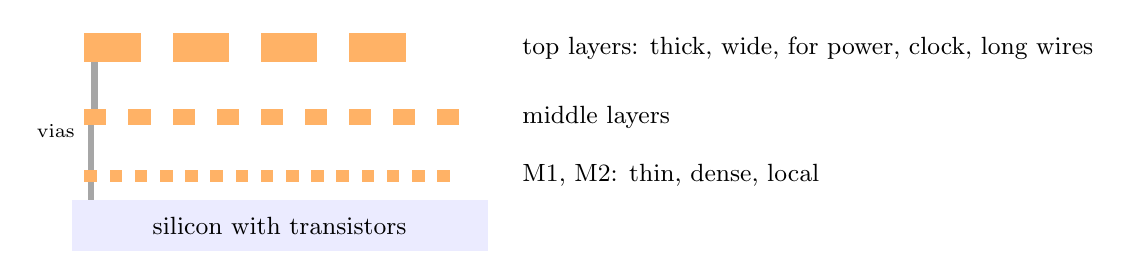
\begin{tikzpicture}[scale=0.8]
  \fill[blue!8] (0,0) rectangle (6.6,0.8); \node at (3.3,0.4) {\small silicon with transistors};
  \foreach \x in {0.2,0.6,...,6.2} \fill[orange!60] (\x,1.1) rectangle (\x+0.2,1.28);
  \foreach \x in {0.2,0.9,...,6.1} \fill[orange!60] (\x,2.0) rectangle (\x+0.35,2.25);
  \foreach \x in {0.2,1.6,...,5.8} \fill[orange!60] (\x,3.0) rectangle (\x+0.9,3.45);
  \fill[gray!70] (0.25,0.8) rectangle (0.35,1.1);
  \fill[gray!70] (0.25,1.28) rectangle (0.35,2.0);
  \fill[gray!70] (0.3,2.25) rectangle (0.42,3.0);
  \node[left,font=\scriptsize] at (0.2,1.9) {vias};
  \node[anchor=west,font=\small] at (7.0,1.2) {M1, M2: thin, dense, local};
  \node[anchor=west,font=\small] at (7.0,2.12) {middle layers};
  \node[anchor=west,font=\small] at (7.0,3.22) {top layers: thick, wide, for power, clock, long wires};
\end{tikzpicture}
\caption{Wiring layers above the transistors (not to scale). Lower layers are thin and closely packed; upper layers are thick and widely spaced.}
\label{fig:metalstack}
\end{figure}

\begin{itemize}
  \item The \textbf{lowest layers} are thin and densely packed, for short connections between nearby transistors.
  \item The \textbf{highest layers} are thick and wide. They carry power, ground, the clock, and long signals that cross the chip, because thick wires have much lower resistance.
  \item Modern chips use \textbf{copper} wires (lower resistivity than aluminum, and more resistant to electromigration), embedded in \textbf{low-$k$} insulators that reduce capacitance between wires.
\end{itemize}

\section{Wire resistance}

A wire's resistance is $R = \rho L/(W T)$, with length $L$, width $W$ and thickness $T$. Since all wires on one layer have the same thickness, designers use the layer's \term{sheet resistance} $R_\square = \rho/T$, in ohms per square. A wire's resistance is then its sheet resistance times the number of \emph{squares} it contains, length divided by width:
\[
  R = R_\square \cdot \frac{L}{W}.
\]
(A square of any size has the same resistance: a bigger square is longer, but proportionally wider.)

\begin{worked}{resistance of a thin wire}
A wire on a lower layer is 1\,mm long and 50\,nm wide, with a sheet resistance of 0.2\,$\Omega/\square$.
Squares: $10^{-3}/(50\times10^{-9}) = 20{,}000$. Resistance: $0.2 \times 20{,}000 = 4$\,k$\Omega$, comparable to a transistor's resistance. Long thin wires are slow.
\end{worked}

At these tiny dimensions, copper's effective resistivity is also higher than in bulk copper, because electrons scatter off the wire's surfaces and grain boundaries, and part of the cross-section is taken up by a barrier liner. Wire resistance is one of the hardest problems in advanced chips.

\section{Wire capacitance and crosstalk}

A wire has capacitance to the layers above and below (effectively to ground) and to its \emph{neighbors} on the same layer. In dense wiring, neighbor capacitance, called \term{coupling capacitance}, is often the largest part. Coupling causes \term{crosstalk}: a switching wire (the \term{aggressor}) disturbs a nearby wire (the \term{victim}).

\paragraph{Noise on a quiet victim.} If the victim is supposed to hold steady, a switching aggressor pushes charge onto it through the coupling capacitance $C_c$. If the victim's driver did not fight back at all, the victim's voltage would jump by
\[
  \Delta V \approx \VDD\,\frac{C_c}{C_c + C_g},
\]
where $C_g$ is the victim's capacitance to ground. A real driver pulls it back, so the result is a glitch. A large enough glitch can flip a latch or a dynamic node.

\begin{worked}{size of a crosstalk glitch}
$C_c = 10$\,fF, $C_g = 30$\,fF, $\VDD = 0.8$\,V. Worst case: $\Delta V \approx 0.8 \times 10/40 = 0.2$\,V, a quarter of the supply.
\end{worked}

\paragraph{Delay change on a switching victim.} If both wires switch at once:
\begin{itemize}
  \item In \textbf{opposite} directions, the voltage across $C_c$ changes by $2\VDD$, so it acts like $2C_c$ (the Miller effect, Chapter~\ref{ch:delay}): the victim is \emph{slower}.
  \item In the \textbf{same} direction, the voltage across $C_c$ barely changes, so it acts like almost nothing: the victim is \emph{faster}.
\end{itemize}

\paragraph{Switching windows.} Crosstalk only matters if the aggressor switches while the victim is vulnerable. Each net has a \term{switching window}: the interval between the earliest and latest times it can change, found by adding up the shortest and longest delays along the paths that drive it. Two coupled nets can interact only where their windows overlap.

\begin{worked}{do these nets interact?}
Net A can switch anywhere from 1.0\,ns to 1.6\,ns after the clock edge. Net B, which runs next to it, can switch from 1.4\,ns to 2.2\,ns. Their windows overlap from 1.4\,ns to 1.6\,ns, so crosstalk is possible only in that interval. If B's window were 1.8 to 2.2\,ns, there would be no overlap and no timing crosstalk.
\end{worked}

\begin{onoa}
A reported question gives two adjacent nets driven by gates with known delays and asks during what window crosstalk might occur. Compute each net's earliest and latest switching times from its gate delays, then intersect the two intervals.
\end{onoa}

\paragraph{Fixes for crosstalk.} Increase the spacing between wires; put a grounded \term{shield} wire between sensitive wires; route neighbors on different layers or perpendicular to each other; make the victim's driver stronger; or insert buffers to shorten the coupled length.

\section{Signals between chips}

Off the chip, signals travel through package pins, circuit-board traces and connectors. At modern speeds these are transmission lines (Section~\ref{sec:tline}): signals travel as waves, reflections must be prevented by matching impedances and terminating lines, and losses in the board material smear fast edges.

\paragraph{Differential signaling.} Most fast links send each signal on \emph{two} wires carrying opposite voltages, and the receiver looks only at the \emph{difference}. Noise that hits both wires equally (common-mode noise) cancels out. Differential links can therefore use small voltage swings, which saves power and allows very high speeds. PCIe, USB, HDMI, Ethernet and NVIDIA's NVLink all use differential pairs.

\paragraph{SerDes.} Instead of many slow parallel wires that must stay perfectly aligned in time, high-speed links use a few very fast serial lanes. A \term{serializer/deserializer} (SerDes) converts wide parallel data into a fast bit stream and back. The receiver recovers the clock from the data's transitions, so the data is \term{encoded} to guarantee enough transitions: 8b/10b encoding (8 data bits sent as 10, 80\% efficient) or 128b/130b (about 98.5\% efficient).

\paragraph{Eye diagrams.} Engineers check link quality by overlaying many bit periods of the received signal. A clean link shows a wide-open ``eye'' between the 0 and 1 levels; noise, jitter and reflections close it.

\section{Bandwidth calculations}
\label{sec:bandwidth}

Bandwidth questions are mostly careful unit-keeping:
\[
  \text{bandwidth (bytes/s)} = \frac{\text{bus width (bits)} \times \text{transfers per second}}{8} \times \text{efficiency}.
\]

\begin{itemize}
  \item \textbf{DDR} (double data rate) transfers data on both the rising and falling clock edges: two transfers per clock cycle.
  \item Link speeds are often given in \textbf{GT/s} (giga-transfers per second), which for a single lane equals Gb/s before encoding overhead.
  \item Divide bits by 8 for bytes. Apply encoding efficiency and protocol overhead (packet headers) if the question includes them.
\end{itemize}

\begin{worked}{DDR bandwidth}
An 8-bit DDR interface has a 10\,GHz clock. Transfers per second: $2 \times 10^{10}$. Bandwidth: $8 \times 2\times10^{10}/8 = 2\times10^{10}$\,bytes/s $= 20$\,GB/s.

If instead ``10\,GHz'' were the data rate (10\,GT/s, already counting both edges), the answer would be 10\,GB/s. Read carefully which one a question means.
\end{worked}

\begin{worked}{memory and link bandwidth}
\textbf{HBM}: one stack has a 1024-bit interface at 6.4\,Gb/s per pin: $1024 \times 6.4/8 \approx 819$\,GB/s.

\textbf{PCIe}: a 16-lane link at 16\,GT/s per lane with 128b/130b encoding: $16 \times 16 \times (128/130)/8 \approx 31.5$\,GB/s in each direction.

\textbf{Protocol overhead}: if every 256-byte payload travels with 24 bytes of headers, only $256/280 \approx 91\%$ of the link carries data, so the payload rate is 91\% of the raw rate.
\end{worked}

\section{Packets and address alignment}

Links such as PCIe move data in \term{packets} with a maximum payload size. Memory systems also prefer requests that do not cross certain \term{aligned} boundaries (addresses that are multiples of 64 bytes, for example). A large read is therefore split into several reply packets, and the first packet may be short so that later packets start on aligned boundaries.

\begin{worked}{how many reply packets?}
A device reads 202 bytes starting at address \code{0x31121133}. Replies carry at most 64 bytes and must not cross a 64-byte-aligned boundary.

The address's offset within its 64-byte block is its low 6 bits: \code{0x33} $= 51$. The first packet can carry only up to the next boundary: $64 - 51 = 13$ bytes. Remaining: $202 - 13 = 189$ bytes, which takes $\lceil 189/64 \rceil = 3$ more packets (64, 64 and 61 bytes). Total: \textbf{4 packets}.

Here the simple estimate $\lceil 202/64 \rceil = 4$ happens to agree, but not always. A 128-byte read starting at offset 32 needs \emph{three} packets (32, 64, 32), not two.
\end{worked}

\begin{onoa}
A reported question asked for the number of completion packets for a 202-byte read at address \code{0x31121133} with a 64-byte maximum payload. The method above, with alignment, gives 4.
\end{onoa}

\section{Summary}

\begin{itemize}
  \item Lower metal layers are thin and dense; upper layers are thick, for power, clock and long wires.
  \item $R = R_\square \cdot L/W$; very thin wires are surprisingly resistive.
  \item Coupling capacitance causes crosstalk: glitches on quiet victims ($\Delta V \approx \VDD C_c/(C_c+C_g)$) and delay changes on switching ones (opposite directions slower, same direction faster).
  \item Crosstalk needs overlapping switching windows.
  \item Fast chip-to-chip links are differential, serial (SerDes) and encoded.
  \item Bandwidth $=$ width $\times$ transfer rate $/ 8 \times$ efficiency; DDR doubles transfers per clock.
  \item Reads are split into packets at the maximum payload size and at aligned boundaries.
\end{itemize}

\section{Exercises}

\begin{enumerate}
  \item A wire is 200\,$\mu$m long and 0.1\,$\mu$m wide, on a layer with $R_\square = 0.1\,\Omega/\square$. What is its resistance?
  \item $C_c = 5$\,fF, $C_g = 15$\,fF, $\VDD = 0.8$\,V. Estimate the worst-case crosstalk glitch.
  \item Net A switches between 0.2 and 0.5\,ns; net B between 0.6 and 0.9\,ns. Can they cause timing crosstalk?
  \item How does a neighbor switching in the opposite direction affect a victim's delay? In the same direction?
  \item A 32-bit DDR bus runs at a 1.6\,GHz clock. What is its bandwidth?
  \item A PCIe link has 8 lanes at 8\,GT/s with 128b/130b encoding. What is its bandwidth per direction?
  \item A device reads 100 bytes starting at address \code{0x1030}, with 64-byte maximum payloads that cannot cross 64-byte boundaries. How many packets?
  \item Why does differential signaling resist noise?
\end{enumerate}

\subsection*{Answers}
\begin{enumerate}
  \item $2000$ squares $\times\, 0.1 = 200\,\Omega$.
  \item $0.8 \times 5/20 = 0.2$\,V.
  \item No; their windows do not overlap.
  \item Opposite: slower (the coupling acts like double the capacitance). Same: faster.
  \item $32 \times 3.2\times10^9 / 8 = 12.8$\,GB/s.
  \item $8 \times 8 \times (128/130)/8 \approx 7.9$\,GB/s.
  \item Offset of \code{0x1030} in its 64-byte block is \code{0x30} $= 48$, so the first packet carries 16 bytes; the remaining 84 bytes need 2 more (64 and 20). Total 3 packets.
  \item Noise usually couples equally onto both wires of the pair, and the receiver only looks at the difference between them, so the common noise cancels.
\end{enumerate}

\chapter{Manufacturing and Reliability}
\label{ch:fab}

A design that is logically perfect can still fail: it might be damaged while it is being manufactured, wear out after a year in the field, or be destroyed by a spark of static electricity. This chapter explains how chips are made and the physical rules designers follow to keep them alive, including the antenna rule from the assessment.

\section{From sand to wafer}

Chips start as extremely pure silicon, grown into a single crystal cylinder (an ingot) and sliced into thin, polished discs called \term{wafers}, today mostly 300\,mm across. Hundreds of chips (\term{dies}) are built side by side on each wafer.

Manufacturing has two halves:
\begin{itemize}
  \item the \term{front end of line} (FEOL) builds the transistors in and on the silicon;
  \item the \term{back end of line} (BEOL) builds the stack of metal wiring layers above them, one layer at a time from the bottom up (Chapter~\ref{ch:wires}).
\end{itemize}

\section{Photolithography: printing the patterns}

Every layer's pattern is printed using light, much like developing a photograph:
\begin{enumerate}
  \item Coat the wafer with a light-sensitive film, \term{photoresist}.
  \item Shine light through a \term{mask} (or reticle) carrying the layer's pattern, so only some of the resist is exposed.
  \item \term{Develop} the resist, washing away the exposed (or unexposed) parts.
  \item \term{Etch} the material not protected by resist, or implant dopants into it.
  \item Strip the remaining resist, and repeat for the next layer.
\end{enumerate}
A modern chip needs dozens of masks and hundreds of process steps. Features are now far smaller than the wavelength of the light used to print them (193\,nm deep ultraviolet, or 13.5\,nm extreme ultraviolet, EUV), which requires tricks such as \term{optical proximity correction} (deliberately distorting mask shapes so they print correctly) and \term{multi-patterning} (printing one layer with several masks).

\section{Other process steps}

\begin{itemize}
  \item \textbf{Deposition}: growing or depositing thin films of insulator or metal, sometimes one atomic layer at a time.
  \item \textbf{Etching}: removing material, usually with a reactive \term{plasma} (an electrically charged gas). Plasma etching is why the antenna rule exists.
  \item \textbf{Ion implantation}: firing dopant atoms into the silicon to make n-type and p-type regions, followed by \textbf{annealing} (heating) to repair the crystal.
  \item \textbf{Chemical--mechanical polishing} (CMP): grinding each layer perfectly flat before the next. Polishing works evenly only if the density of metal is roughly uniform, so tools add \term{dummy fill}: small unconnected metal shapes in empty areas.
\end{itemize}

\section{Test, dicing and packaging}

Each die on the finished wafer is tested with fine probes. The wafer is cut (diced) into individual dies, and good dies are placed in a \term{package} that connects them to the circuit board, spreads heat and protects them. High-performance chips are mounted face down (\term{flip-chip}) on thousands of tiny solder bumps.

Advanced packaging now matters as much as transistors. Large GPUs place the processor die and stacks of high-bandwidth memory (HBM) side by side on a silicon \term{interposer} full of fine wires (2.5D packaging), and some products stack dies directly on top of each other (3D). Splitting a design into several smaller dies, \term{chiplets}, connected in one package, helps yield, as the next section shows.

\section{Yield}

Tiny defects (a dust particle, a flaw in a film) land randomly across a wafer. A die with a defect in a critical spot does not work. If defects land at an average density $D$ per unit area, the fraction of dies of area $A$ that escape them all is approximately
\[
  Y = e^{-D A}.
\]

\begin{worked}{yield and die size}
With $D = 0.1$ defects per cm$^2$: a 1\,cm$^2$ die has $Y = e^{-0.1} \approx 90\%$. An 8\,cm$^2$ die has $Y = e^{-0.8} \approx 45\%$.
\end{worked}

Large dies are doubly expensive: fewer fit on a wafer, and a smaller fraction of them work. Designers fight back with \textbf{redundancy} (spare memory rows and columns that can replace defective ones) and by \textbf{disabling} defective units (a GPU with one broken processing cluster can be sold as a lower-tier product with that cluster turned off).

\section{The design flow}

The path from an idea to a manufacturable layout:
\begin{enumerate}
  \item Specification and architecture.
  \item RTL design in a hardware description language, and functional verification (Chapter~\ref{ch:rtl}).
  \item \textbf{Synthesis}: tools turn RTL into a netlist of standard cells (gates and flip-flops from a library).
  \item \textbf{Floorplanning}: placing large blocks, memories, I/O and the power grid.
  \item \textbf{Placement} of the standard cells.
  \item \textbf{Clock tree synthesis}.
  \item \textbf{Routing}: connecting everything with metal.
  \item \textbf{Sign-off}: static timing analysis, power and IR-drop analysis, and the physical checks below.
  \item \textbf{Tape-out}: sending the final layout (a GDSII or OASIS file) to the factory.
\end{enumerate}

Key physical checks:
\begin{itemize}
  \item \term{DRC} (design rule check): every shape obeys the factory's geometric rules: minimum widths, spacings, enclosures, densities.
  \item \term{LVS} (layout versus schematic): the transistors and connections in the layout match the intended netlist.
  \item \textbf{Antenna}, \textbf{electromigration} and \textbf{ERC} (electrical rule) checks, described next.
\end{itemize}

\section{The antenna effect}
\label{sec:antenna}

During manufacturing, metal layers are patterned by plasma etching. The plasma is full of charged particles, and any metal wire exposed to it collects charge, like an antenna collecting a radio signal. The longer (larger in area) the wire, the more charge it collects.

Normally that charge would drain away harmlessly through a transistor's source or drain diffusion, which connects to the silicon. But consider a wire, being built on a lower metal layer, whose only connection so far is to the \emph{gate} of a transistor (Figure~\ref{fig:antenna}). The connection to the driving gate's output, which would provide a diffusion path, may only be completed later, on a higher metal layer that does not exist yet. The collected charge has nowhere to go except \emph{through the thin gate oxide}. Enough charge forced through the oxide damages it: it shifts the transistor's threshold voltage, makes the oxide leaky, or breaks it down completely.

\begin{figure}[h]
\centering
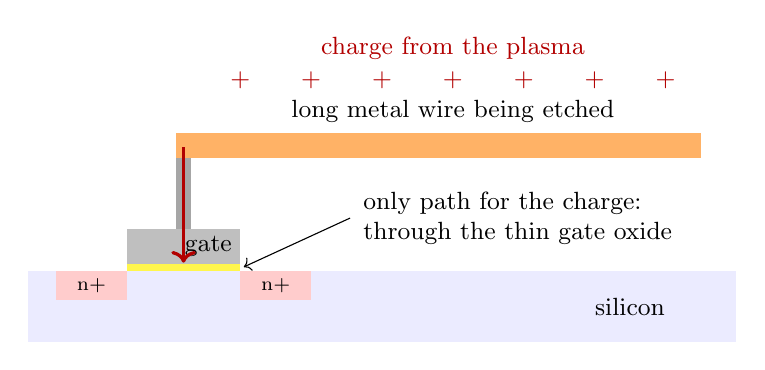
\begin{tikzpicture}[scale=0.9]
  \fill[blue!8] (0,0) rectangle (10,1); \node at (8.5,0.5) {\small silicon};
  \fill[red!20] (0.4,0.6) rectangle (1.4,1); \fill[red!20] (3.0,0.6) rectangle (4.0,1);
  \node[font=\scriptsize] at (0.9,0.8) {n+}; \node[font=\scriptsize] at (3.5,0.8) {n+};
  \fill[yellow!70] (1.4,1) rectangle (3.0,1.1);
  \fill[gray!50] (1.4,1.1) rectangle (3.0,1.6); \node[font=\small] at (2.55,1.35) {gate};
  \fill[gray!70] (2.1,1.6) rectangle (2.3,2.6);
  \fill[orange!60] (2.1,2.6) rectangle (9.5,2.95);
  \node[font=\small] at (6,3.25) {long metal wire being etched};
  \foreach \x in {3,4,...,9} \node[red!70!black,font=\small] at (\x,3.7) {$+$};
  \node[font=\small,red!70!black] at (6,4.15) {charge from the plasma};
  \draw[->,very thick,red!70!black] (2.2,2.75) -- (2.2,1.12);
  \node[font=\small,anchor=west,align=left] at (4.6,1.75) {only path for the charge:\\through the thin gate oxide};
  \draw[->] (4.55,1.75) -- (3.05,1.06);
\end{tikzpicture}
\caption{The antenna effect: a long wire connected only to a gate funnels plasma charge through the gate oxide.}
\label{fig:antenna}
\end{figure}

\paragraph{The antenna rule.} The danger depends on how much charge is collected compared with how much oxide area it is spread over. So the rule limits the \term{antenna ratio}:
\[
  \text{antenna ratio} = \frac{\text{area of metal connected to the gate (during that etch)}}{\text{area of the gate oxide it connects to}}.
\]
The factory gives a maximum ratio for each layer. Notice what each side means:
\begin{itemize}
  \item More metal (a longer wire) collects more charge: \textbf{worse}.
  \item More gate area spreads the charge over more oxide: \textbf{better}.
\end{itemize}

\begin{onoa}
The assessment asked, true or false: ``For the antenna rule, as long as the metal wire is safe, a small connected transistor is good.'' This is \textbf{false}. The wire is not ``safe'' or ``unsafe'' on its own; what matters is the \emph{ratio} of metal area to gate area. A \emph{smaller} gate means a \emph{larger} ratio, so a small connected transistor makes an antenna violation \emph{more} likely. A larger gate (or several gates) on the same wire is safer.
\end{onoa}

\paragraph{Fixing antenna violations.}
\begin{itemize}
  \item \textbf{Antenna diode}: add a small diode from the wire to the substrate near the gate. During etching it gives the charge a safe path to the silicon. In normal operation the diode is reverse biased, so it only adds a little leakage and capacitance (Chapter~\ref{ch:semis}).
  \item \textbf{Metal jumper (layer hopping)}: break the long wire and route part of it on a higher layer. While the lower layer is etched, the gate sees only a short piece of metal; by the time the higher layer is etched, the connection to the driver's diffusion is complete and the charge can drain.
  \item \textbf{Buffer insertion}: insert a buffer near the vulnerable gate, splitting the long wire into two nets, each with a smaller ratio.
  \item \textbf{Larger gate area}: a bigger receiving transistor lowers the ratio (at a cost in power and loading).
\end{itemize}

\section{Electromigration}

Electrons flowing through a wire collide with its metal atoms and, very slowly, push them along in the direction of electron flow. Over months and years this \term{electromigration} (EM) leaves \term{voids} where atoms have left (which can break the wire open) and \term{hillocks} where they pile up (which can short to a neighbor).

The median time to failure follows \term{Black's equation}:
\[
  \text{MTTF} = A\,J^{-n}\,e^{E_a/kT},
\]
where $J$ is the current density, $n$ is typically around 2, $E_a$ is an activation energy, and $T$ is absolute temperature. Two lessons: higher current density shortens life sharply, and higher temperature shortens it \emph{exponentially}.

Wires that carry steady current in one direction (power and ground) are most at risk; signal wires, whose current flows back and forth, are less so. Designers prevent EM failures by limiting current density: wider wires, more parallel wires, and multiple vias at every connection. Copper's better EM resistance was one reason it replaced aluminum.

\section{Latch-up}

A CMOS chip accidentally contains a parasitic structure that can short the supply to ground. Follow the layers from $\VDD$ to ground through a PMOS and a nearby NMOS: the PMOS's p+ source, the n-well, the p-type substrate, and the NMOS's n+ source. That is p-n-p-n, a four-layer device called a \term{thyristor} (or SCR), which behaves like two bipolar transistors feeding each other.

\begin{figure}[h]
\centering
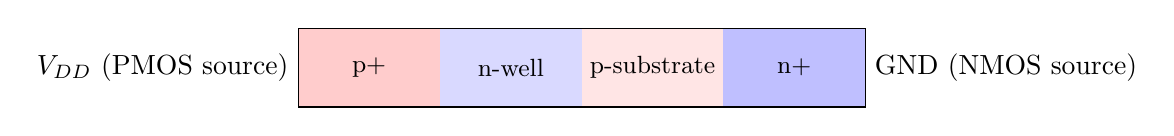
\begin{tikzpicture}
  \foreach \x/\lab/\col in {0/p+/red!20, 1.8/n-well/blue!15, 3.6/p-substrate/red!10, 5.4/n+/blue!25}
    { \fill[\col] (\x,0) rectangle (\x+1.8,1); \node at (\x+0.9,0.5) {\small \lab}; }
  \draw (0,0) rectangle (7.2,1);
  \node[left] at (0,0.5) {$\VDD$ (PMOS source)};
  \node[right] at (7.2,0.5) {GND (NMOS source)};
\end{tikzpicture}
\caption{The parasitic p-n-p-n path inside CMOS. Once triggered, it can latch into a low-resistance state between the supply and ground.}
\end{figure}

Normally this structure is off. But a disturbance that injects current into the well or substrate, such as a voltage spike on an input pin, an ESD event or a radiation strike, can turn both parasitic transistors on. Each then keeps the other on: the structure \emph{latches}, conducting heavily from $\VDD$ to ground until power is removed, often destroying the chip.

\paragraph{Prevention.} Keep the well and substrate firmly tied to their supplies with frequent \term{well taps} and \term{substrate taps} (low resistance there keeps the parasitic transistors from turning on); surround sensitive or I/O transistors with \term{guard rings}; keep NMOS and PMOS devices apart; or use processes that isolate transistors completely (such as silicon-on-insulator).

\section{Electrostatic discharge}

Walking across a carpet can charge your body to thousands of volts. Touching a chip's pin discharges that through the chip in nanoseconds. Gate oxides break down at only a few volts, so an unprotected input would be destroyed instantly. Every I/O pad therefore has \term{ESD protection}: diodes from the pad to $\VDD$ and to ground, plus clamp circuits between the supplies, which steer the discharge current around the core circuitry. ESD structures add capacitance to every pin, which is a challenge for very high-speed I/O.

\section{Aging and soft errors}

\paragraph{Wear-out.} Transistors degrade slowly under voltage and heat:
\begin{itemize}
  \item \term{NBTI} (negative bias temperature instability): PMOS thresholds rise over time while the transistor is on.
  \item \term{HCI} (hot-carrier injection): fast-moving carriers get trapped in the gate oxide, degrading the transistor.
  \item \term{TDDB} (time-dependent dielectric breakdown): the gate oxide eventually wears out under a strong electric field.
\end{itemize}
Designs include an \textbf{aging guardband} in their timing so they still work after years.

\paragraph{Soft errors.} A neutron from cosmic rays, or an alpha particle from trace radioactive impurities, can deposit enough charge to flip a bit in an SRAM cell or a flip-flop without damaging anything. These \term{soft errors} are handled with parity and error-correcting codes (Chapter~\ref{ch:memory}).

\section{Testing manufactured chips}

Factory testing looks for manufacturing defects, not design bugs. The standard model is the \term{stuck-at fault}: a node permanently stuck at 0 or 1. Scan chains (Chapter~\ref{ch:latch}) let testers load every flip-flop with a pattern, run one clock cycle, and read every result back out. Software (\term{ATPG}, automatic test pattern generation) finds a small set of patterns that detect nearly all possible stuck-at faults. Memories have built-in self-test (\term{BIST}) circuits that run test patterns on themselves.

\section{Summary}

\begin{itemize}
  \item Chips are printed layer by layer with photolithography; transistors first (FEOL), then wires (BEOL).
  \item Yield falls exponentially with die area ($Y = e^{-DA}$), motivating redundancy and chiplets.
  \item DRC checks shapes; LVS checks that the layout matches the netlist.
  \item Antenna effect: plasma charge on a wire connected only to a gate flows through the gate oxide. The rule limits metal area / gate area; a small gate is \emph{worse}. Fixes: diodes, layer jumpers, buffers, larger gates.
  \item Electromigration: current density and heat move metal atoms; MTTF $\propto J^{-n}e^{E_a/kT}$.
  \item Latch-up: a parasitic p-n-p-n thyristor shorts $\VDD$ to ground; prevented by taps and guard rings.
  \item ESD protection diodes guard every pin.
  \item Aging (NBTI, HCI, TDDB) needs guardbands; soft errors need ECC.
\end{itemize}

\section{Exercises}

\begin{enumerate}
  \item True or false: for the antenna rule, as long as the metal wire is safe, a small connected transistor is good. Explain.
  \item Give two ways to fix an antenna violation.
  \item With a defect density of 0.2 per cm$^2$, what is the yield of a 2\,cm$^2$ die?
  \item Does electromigration get better or worse at higher temperature?
  \item What causes latch-up, and name two ways to prevent it.
  \item What is the difference between DRC and LVS?
  \item Why do layout tools add dummy metal fill?
  \item What protects a chip's input pins from static electricity?
  \item Why does doubling a die's area more than double its cost per working die?
\end{enumerate}

\subsection*{Answers}
\begin{enumerate}
  \item False. The risk depends on the ratio of metal area to gate area. A smaller gate gives a larger ratio, so the charge collected by the wire is concentrated on less oxide: more likely to cause damage.
  \item Any two of: an antenna diode near the gate; breaking the wire and jumping to a higher metal layer; inserting a buffer near the gate; increasing the gate area.
  \item $e^{-0.4} \approx 67\%$.
  \item Worse; lifetime falls exponentially as temperature rises.
  \item A parasitic p-n-p-n structure (two coupled parasitic bipolar transistors) between the PMOS and NMOS can be triggered by injected current and then holds a low-resistance path from $\VDD$ to ground. Prevent it with frequent well and substrate taps, guard rings, spacing, or isolated processes such as SOI.
  \item DRC checks that layout shapes obey the factory's geometric rules. LVS checks that the circuit extracted from the layout matches the intended schematic or netlist.
  \item To make the metal density uniform so chemical-mechanical polishing produces flat layers.
  \item ESD protection: diodes from each pad to the supply and ground, plus supply clamps, that divert the discharge current.
  \item Fewer dies fit on each wafer, and the fraction of working dies falls (yield $e^{-DA}$ drops as $A$ grows), so both effects raise the cost of each good die.
\end{enumerate}

\chapter{Memory Circuits}
\label{ch:memory}

A large part of every GPU's silicon is memory: register files, caches, shared memory. Off the chip sit gigabytes of DRAM. Flip-flops (Chapter~\ref{ch:latch}) are far too big to store that much, so memories use specialized, tiny storage cells packed into dense arrays. This chapter explains the two workhorse cells, SRAM and DRAM, and the circuits around them.

\section{Kinds of memory}

\begin{center}
\small
\begin{tabularx}{\linewidth}{>{\raggedright\arraybackslash}p{2.6cm}*{4}{>{\raggedright\arraybackslash}X}}
\toprule
 & Flip-flop & SRAM & DRAM & Flash \\
\midrule
Cell & 20+ transistors & 6 transistors & 1 transistor, 1 capacitor & 1 special transistor \\
Speed & fastest & very fast & medium & slow (writes very slow) \\
Density & lowest & low & high & highest \\
Needs refresh & no & no & yes & no \\
Keeps data without power & no & no & no & yes \\
Typical use & pipeline registers & caches, register files & main and GPU memory & SSDs, storage \\
\bottomrule
\end{tabularx}
\end{center}

Memory that loses its contents without power is \term{volatile} (SRAM, DRAM); memory that keeps them is \term{nonvolatile} (flash).

\section{How a memory array is organized}

Memory cells are arranged in a grid (Figure~\ref{fig:array}):
\begin{itemize}
  \item Each \textbf{row} shares a horizontal \term{wordline}. Turning a wordline on connects every cell in that row to its column.
  \item Each \textbf{column} shares a vertical \term{bitline} (in SRAM, a pair: $BL$ and $\nt{BL}$), which carries data in and out.
  \item A \term{row decoder} turns the row part of the address into one active wordline (Chapter~\ref{ch:comb}).
  \item \term{Sense amplifiers} at the bottom of the columns detect the small signals the cells put on the bitlines; a \term{column multiplexer} picks which columns are the requested word.
\end{itemize}

\begin{figure}[h]
\centering
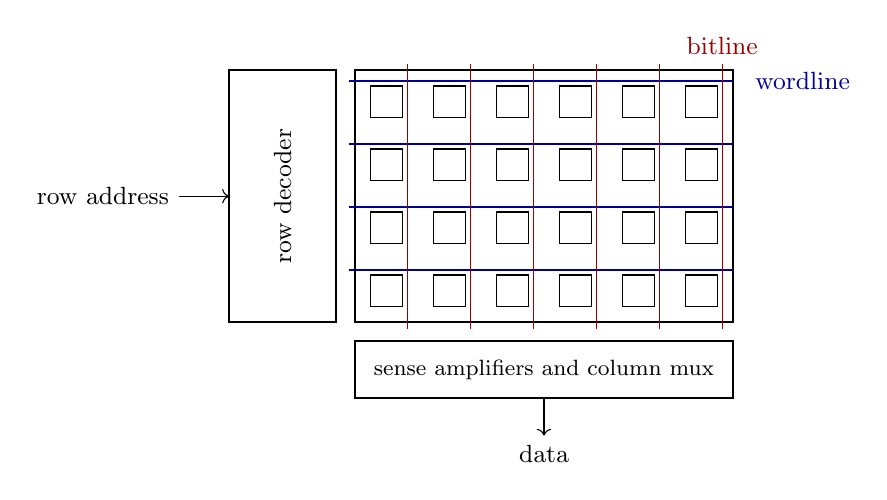
\begin{tikzpicture}[scale=0.8]
  \draw[thick] (0,0) rectangle (6,4);
  \foreach \x in {0.5,1.5,...,5.5} \foreach \y in {0.5,1.5,...,3.5} \draw (\x-0.25,\y-0.25) rectangle (\x+0.25,\y+0.25);
  \foreach \y in {0.5,1.5,...,3.5} \draw[blue!60!black] (-0.1,\y+0.33) -- (6,\y+0.33);
  \foreach \x in {0.5,1.5,...,5.5} \draw[red!60!black] (\x+0.33,4.1) -- (\x+0.33,-0.1);
  \draw[thick] (-2,0) rectangle (-0.3,4); \node[rotate=90,align=center,font=\small] at (-1.15,2) {row decoder};
  \draw[thick] (0,-1.2) rectangle (6,-0.3); \node[font=\footnotesize] at (3,-0.75) {sense amplifiers and column mux};
  \draw[<-] (-2,2) -- (-2.8,2) node[left,font=\small]{row address};
  \draw[->] (3,-1.2) -- (3,-1.8) node[below,font=\small]{data};
  \node[blue!60!black,font=\small,anchor=west] at (6.2,3.83) {wordline};
  \node[red!60!black,font=\small,anchor=south] at (5.83,4.1) {bitline};
\end{tikzpicture}
\caption{A memory array: wordlines select a row; bitlines carry data to the sense amplifiers.}
\label{fig:array}
\end{figure}

\begin{worked}{address bits}
A 256\,Kb ($2^{18}$ bits) SRAM array has 512 rows. Each row then holds $2^{18}/2^9 = 512$ bits. If a word is 32 bits, each row holds 16 words. The address needs $\log_2 512 = 9$ row bits and $\log_2 16 = 4$ column bits: 13 bits to choose one of $2^{13} = 8192$ words.
\end{worked}

\section{The 6T SRAM cell}

An SRAM (static RAM) cell is a bistable loop of two cross-coupled inverters (four transistors) plus two NMOS \term{access transistors} that connect the loop's two nodes to the bitlines when the wordline is high (Figure~\ref{fig:sram}).

\begin{figure}[h]
\centering
\begin{circuitikz}
  \draw (0,0.8) node[not port](i1){};
  \draw (0,-0.8) node[not port, xscale=-1](i2){};
  \draw (i1.out) -- ++(0.4,0) coordinate(r1) -- (r1 |- i2.in) -- (i2.in);
  \draw (i2.out) -- ++(-0.4,0) coordinate(l1) -- (l1 |- i1.in) -- (i1.in);
  \coordinate (qn) at (l1 |- 0,0);
  \coordinate (qbn) at (r1 |- 0,0);
  \fill (qn) circle (0.05); \fill (qbn) circle (0.05);
  \draw (qn) -- ++(-0.6,0) node[nmos, rotate=90, anchor=S](ma){};
  \draw (qbn) -- ++(0.6,0) node[nmos, rotate=90, anchor=D](mb){};
  \draw (ma.D) -- ++(-0.5,0) coordinate(bl);
  \draw (mb.S) -- ++(0.5,0) coordinate(blb);
  \draw (bl |- 0,2.0) node[above]{$BL$} -- (bl |- 0,-2.4);
  \draw (blb |- 0,2.0) node[above]{$\nt{BL}$} -- (blb |- 0,-2.4);
  \draw (ma.G) -- (ma.G |- 0,-1.9);
  \draw (mb.G) -- (mb.G |- 0,-1.9);
  \draw[blue!60!black] ($(bl |- 0,-1.9)+(-0.6,0)$) node[left]{$WL$} -- ($(blb |- 0,-1.9)+(0.6,0)$);
  \node[font=\small,above left] at (qn) {$Q$};
  \node[font=\small,above right] at (qbn) {$\nt{Q}$};
\end{circuitikz}
\caption{A 6T SRAM cell: two cross-coupled inverters store $Q$ and $\nt{Q}$; two access transistors connect them to the bitlines when the wordline $WL$ is high.}
\label{fig:sram}
\end{figure}

\paragraph{Holding.} With the wordline off, the access transistors are off and the loop holds its value indefinitely, as long as power is on. No refresh is needed, which is what ``static'' means.

\paragraph{Reading.} Both bitlines are first \term{precharged} to $\VDD$. Then the wordline turns on. Suppose $Q = 0$. Node $Q$'s side now has a path from the precharged bitline $BL$, through the access transistor and the inverter's pull-down NMOS, to ground, so $BL$ starts to discharge. The other bitline stays high. A sense amplifier detects which bitline is falling, long before it has fallen far.

\paragraph{Read stability.} During that read, node $Q$ (supposed to be 0) is caught in a tug-of-war: the access transistor pulls it up toward the precharged bitline, while the pull-down NMOS pulls it to ground. It is a voltage divider (Chapter~\ref{ch:electricity}), so $Q$ rises a little. If it rises above the other inverter's switching threshold, the cell flips and the read destroys the data (a \term{read upset}). To prevent this, \textbf{the pull-down NMOS must be stronger than the access NMOS}. Their strength ratio is the \term{cell ratio}, typically 1.5 to 2.5.

\paragraph{Writing.} To write $Q = 0$, drive $BL$ to 0 and $\nt{BL}$ to $\VDD$, then turn on the wordline. The access transistor on the $Q$ side must pull $Q$ down \emph{against} the pull-up PMOS that is holding it at 1. So \textbf{the access NMOS must be stronger than the pull-up PMOS} (the \term{pull-up ratio}). Conveniently, PMOS transistors are naturally weaker.

\begin{bigidea}
SRAM cell sizing is a balance: pull-down NMOS $>$ access NMOS $>$ pull-up PMOS. A strong access transistor makes writing easy but reading risky; a weak one makes reading safe but writing hard.
\end{bigidea}

The cell's robustness is measured by its \term{static noise margin} (SNM), read from a plot of the two inverters' transfer curves (the ``butterfly curve''). Process variation (Chapter~\ref{ch:pvt}) makes some cells much weaker than others, which sets the lowest voltage a memory can run at, its $V_{min}$. Some designs use an \textbf{8T cell} with a separate read port that never disturbs the storage nodes, removing the read-stability problem at the cost of area.

\section{Sense amplifiers}

A bitline connects to hundreds of cells, so it has a large capacitance, while each cell's transistors are tiny. Waiting for a cell to swing a bitline all the way to 0 would be very slow. Instead, a \term{sense amplifier} detects a small difference between $BL$ and $\nt{BL}$, often around 100\,mV, and amplifies it to a full logic level. A common design is itself a pair of cross-coupled inverters: released when the bitlines are slightly apart, it quickly regenerates the difference into a full 0 and 1.

\section{DRAM}

A \term{DRAM} (dynamic RAM) cell is one transistor and one capacitor (1T1C). The bit is stored as charge on the capacitor: charged means 1, empty means 0. This is far smaller than an SRAM cell, which is why DRAM provides gigabytes cheaply.

\paragraph{Reading by charge sharing.} The bitline is precharged to $\VDD/2$. Turning on the wordline connects the cell capacitor $C_s$ to the much larger bitline capacitance $C_{BL}$. Charge redistributes, and the bitline moves slightly up (if the cell held a 1) or down (if it held a 0):
\[
  \Delta V = \left(V_{cell} - \frac{\VDD}{2}\right)\frac{C_s}{C_s + C_{BL}}.
\]

\begin{worked}{how big is a DRAM read signal?}
$C_s = 20$\,fF, $C_{BL} = 80$\,fF, $\VDD = 1.2$\,V, and the cell holds a 1 (1.2\,V). The bitline starts at 0.6\,V.
\[
  \Delta V = (1.2 - 0.6) \times \frac{20}{20 + 80} = 0.6 \times 0.2 = 0.12~\text{V}.
\]
Only 120\,mV, which a sense amplifier must detect.
\end{worked}

\paragraph{Destructive reads.} Charge sharing disturbs the cell's own charge, so every read destroys the stored value. The sense amplifier, once it has decided, drives the bitline to a full level, which writes the value back into the cell.

\paragraph{Refresh.} The capacitor slowly leaks its charge. Every cell must be read and rewritten periodically, typically every 64\,ms, which is called \term{refresh}. Refresh costs power and briefly blocks access. That periodic refresh is what ``dynamic'' means.

\paragraph{DRAM organization.} A DRAM chip is divided into \term{banks}. Accessing data first opens a whole row into a \term{row buffer} (slow), after which columns from that open row can be read quickly. Accesses that hit an already open row are much faster than those that need a new row. Graphics memory (GDDR) and high-bandwidth memory (HBM, stacks of DRAM dies next to the GPU) are DRAM organized for very high bandwidth (Chapter~\ref{ch:wires}).

\section{Flash memory}

A \term{flash} cell is a transistor with an extra, electrically isolated gate (a floating gate or a charge-trapping layer) under its control gate. Electrons forced onto that layer by tunneling at high voltage stay there for years without power and shift the transistor's threshold voltage. Reading measures the threshold. Flash is nonvolatile and very dense (cells can store 2, 3 or 4 bits by distinguishing several threshold levels), but writing is slow, it must be erased in large blocks, and each cell survives only a limited number of write cycles. It is used for storage (SSDs), not as working memory.

\section{Register files, CAMs and ROMs}

\begin{itemize}
  \item A \term{register file} is a small, very fast SRAM with many \term{ports}, so several registers can be read and written in the same cycle. Each extra port adds wordlines, bitlines and access transistors to every cell, so ports are expensive. GPUs have very large register files to hold the state of thousands of threads (Chapter~\ref{ch:gpu}).
  \item A \term{content-addressable memory} (CAM) works backwards: you give it a value and it reports which entries contain it, comparing all entries in parallel. CAMs are used in translation lookaside buffers and network routers. They are fast but power-hungry.
  \item A \term{read-only memory} (ROM) holds fixed contents set at manufacture.
\end{itemize}

\section{Protecting stored data: ECC}

Soft errors (Chapter~\ref{ch:fab}) can flip stored bits. A single \term{parity} bit (the XOR of all data bits) detects any single-bit error but cannot say which bit flipped. \term{Error-correcting codes} add more check bits. The common SECDED code (single-error correct, double-error detect) protects 64 data bits with 8 check bits, which is why server and GPU memory often has 72-bit-wide words. Memories may also \term{scrub}: periodically read, correct and rewrite every word so errors do not accumulate.

\section{Summary}

\begin{itemize}
  \item Memory arrays: wordlines select rows, bitlines carry data, decoders select rows, sense amps detect small signals.
  \item 6T SRAM: two cross-coupled inverters plus two access NMOS. Static: no refresh.
  \item Read stability needs pull-down $>$ access; writability needs access $>$ pull-up.
  \item Sense amplifiers turn ~100\,mV bitline differences into full logic levels.
  \item DRAM: 1T1C, read by charge sharing ($\Delta V = (V_{cell} - \VDD/2)\,C_s/(C_s + C_{BL})$), destructive reads, refresh every ~64\,ms.
  \item Flash: nonvolatile, dense, slow to write, limited endurance.
  \item Parity detects single errors; SECDED ECC (64 + 8 bits) corrects them.
\end{itemize}

\section{Exercises}

\begin{enumerate}
  \item How many transistors are in a standard SRAM cell? What are they?
  \item For read stability, which must be stronger: the pull-down NMOS or the access NMOS? Why?
  \item For writability, which must be stronger: the access NMOS or the pull-up PMOS?
  \item A DRAM cell of 30\,fF holding a 1 (1.0\,V) is read onto a 120\,fF bitline precharged to 0.5\,V. Find the bitline change.
  \item Why does DRAM need refresh? Why does SRAM not?
  \item Is a DRAM read destructive? An SRAM read?
  \item A 256\,Kb array has 512 rows and 32-bit words. How many row and column address bits are needed?
  \item How many check bits does SECDED use for 64 data bits?
  \item Why are sense amplifiers needed instead of waiting for full bitline swings?
  \item Which memory keeps its data with power off: SRAM, DRAM or flash?
\end{enumerate}

\subsection*{Answers}
\begin{enumerate}
  \item Six: two PMOS pull-ups and two NMOS pull-downs forming two cross-coupled inverters, plus two NMOS access transistors.
  \item The pull-down. During a read, the 0 node is a voltage divider between them; a stronger pull-down keeps the node low enough that the cell does not flip.
  \item The access NMOS, so it can overpower the PMOS holding the node at 1.
  \item $(1.0 - 0.5) \times 30/150 = 0.1$\,V.
  \item The DRAM capacitor leaks its charge over time. SRAM's cross-coupled inverters actively hold the value from the supply.
  \item DRAM: yes (charge sharing disturbs the cell; it is written back). SRAM: no (if correctly sized).
  \item $2^{18}/512 = 512$ bits per row, so 16 words per row: 9 row bits and 4 column bits.
  \item 8.
  \item Bitlines have large capacitance and cells are tiny, so a full swing would take far too long; sensing a ~100\,mV difference is much faster.
  \item Flash.
\end{enumerate}


\part{Digital Systems}
\chapter{Describing and Verifying Hardware: RTL, Verilog, Clock Domains and FIFOs}
\label{ch:rtl}

Nobody draws a billion transistors by hand. Digital designers describe hardware in a \term{hardware description language} (HDL), most often Verilog or SystemVerilog, at the \term{register-transfer level} (RTL): registers, and the logic that computes their next values. Tools then turn that description into gates (synthesis) and the gates into layout. This chapter covers the HDL ideas that hardware questions test, two design problems that come up constantly (crossing between clock domains, and sizing FIFOs), and finally how designs are verified before they are built.

\section{An HDL describes hardware, not steps}

Verilog looks like a programming language, but it is not one. A program is a list of steps executed one after another. An HDL describes \emph{circuits that all exist at once}, every gate working in parallel all the time. A line of Verilog does not ``run''; it describes a piece of hardware that is always there.

\section{Verilog in one page}

\begin{lstlisting}[language=Verilog]
module mux2 (
  input  wire       s,
  input  wire [7:0] a, b,     // 8-bit buses, bit 7 is the MSB
  output wire [7:0] y
);
  assign y = s ? b : a;       // continuous assignment: combinational logic
endmodule
\end{lstlisting}

\begin{itemize}
  \item A \code{module} is a block of hardware with \code{input} and \code{output} ports. Modules are instantiated inside other modules to build hierarchy.
  \item \code{[7:0]} declares an 8-bit bus. \code{\{a, b\}} concatenates buses; \code{a[3:0]} selects bits.
  \item \code{assign} describes combinational logic that is always active.
  \item An \code{always @(*)} block also describes combinational logic, using \code{if} and \code{case}.
  \item An \code{always @(posedge clk)} block describes flip-flops: everything assigned inside updates on the rising clock edge.
\end{itemize}

\begin{lstlisting}[language=Verilog]
module counter4 (
  input  wire       clk, rst_n, en,
  output reg  [3:0] count
);
  always @(posedge clk or negedge rst_n) begin
    if (!rst_n)      count <= 4'd0;          // asynchronous, active-low reset
    else if (en)     count <= count + 4'd1;  // count when enabled
  end
endmodule
\end{lstlisting}

(In Verilog, a signal assigned in an \code{always} block is declared \code{reg}; that does not necessarily mean it becomes a register. SystemVerilog replaces both \code{wire} and \code{reg} with \code{logic}. It also adds \code{always\_ff} and \code{always\_comb}, which state the designer's intent, so tools can warn when the code does not really describe flip-flops or pure combinational logic, for example when an \code{always\_comb} block would infer a latch.)

\section{Blocking and nonblocking assignments}
\label{sec:blocking}

Verilog has two assignment operators inside \code{always} blocks, and confusing them is the most famous Verilog bug.

\begin{itemize}
  \item \textbf{Blocking} \code{=}: the assignment happens immediately, and the next statement sees the new value, like a programming language.
  \item \textbf{Nonblocking} \code{<=}: the right-hand sides are all evaluated first, using the old values, and all the left-hand sides are updated together at the end of the time step, like flip-flops all capturing on the same clock edge.
\end{itemize}

\begin{worked}{swapping two registers}
Start with \code{a = 1}, \code{b = 2}.

\textbf{Nonblocking:}
\begin{lstlisting}[language=Verilog]
always @(posedge clk) begin
  a <= b;
  b <= a;
end
\end{lstlisting}
Both right sides use the old values: after the first edge \code{a = 2, b = 1}; after the second \code{a = 1, b = 2}. The registers swap every cycle, which is what two cross-connected flip-flops do.

\textbf{Blocking:}
\begin{lstlisting}[language=Verilog]
always @(posedge clk) begin
  a = b;    // a becomes 2 immediately
  b = a;    // reads the NEW a, so b becomes 2
end
\end{lstlisting}
After the first edge \code{a = 2, b = 2}, and they stay 2 forever. No swap.
\end{worked}

\begin{worked}{what does \code{\$display} print?}
\begin{lstlisting}[language=Verilog]
always @(posedge clk) begin
  a <= b;
  b <= a;
  $display("a=%0d b=%0d", a, b);
end
\end{lstlisting}
With \code{a = 1, b = 2} initially, the first edge prints \code{a=1 b=2}, not the swapped values: nonblocking updates happen at the \emph{end} of the time step, after \code{\$display} has already run. The second edge prints \code{a=2 b=1}.
\end{worked}

\begin{onoa}
A reported question shows an \code{always} block with blocking and nonblocking assignments and asks what values of \code{a} and \code{b} are displayed in the first and second cycles. Work through it as above: blocking updates are seen by the following statements immediately; nonblocking updates are not visible until the time step ends.
\end{onoa}

\begin{remember}
Use \code{<=} (nonblocking) in clocked \code{always @(posedge clk)} blocks. Use \code{=} (blocking) in combinational \code{always @(*)} blocks. Never mix them in one block.
\end{remember}

\section{Accidental latches}

In a combinational \code{always @(*)} block, every output must be assigned a value in \emph{every} path through the code. If some path leaves an output unassigned, the output must ``remember'' its old value, and synthesis creates a latch, usually unintended.

\begin{lstlisting}[language=Verilog]
always @(*) begin
  if (sel) y = a;        // no else: when sel is 0, y must hold its value
end                      //   -> a latch is inferred
\end{lstlisting}
The fix: add the \code{else}, give a \code{default} in every \code{case}, or assign a default value at the top of the block.

\section{Resets}

\paragraph{Synchronous reset.} The reset is just another input to the logic in front of the flip-flops: \code{if (rst) q <= 0;} inside \code{always @(posedge clk)}. It takes effect at the next clock edge, so it needs a running clock, but it never causes timing surprises.

\paragraph{Asynchronous reset.} The reset is in the sensitivity list (\code{always @(posedge clk or negedge rst\_n)}) and drives the flip-flops' clear pins directly, so it works with no clock. The danger is \emph{releasing} it: if reset deasserts close to a clock edge, some flip-flops may leave reset one cycle earlier than others, or go metastable. The standard solution is a \term{reset synchronizer}: assert reset asynchronously, but release it through two flip-flops clocked by the destination clock (``asynchronous assert, synchronous deassert'').

\paragraph{Filtering glitches on a reset line.} A noisy reset input should not reset the chip because of a brief glitch. One simple filter compares the reset with a delayed copy of itself: for an active-low reset, the filtered reset is asserted only when both the input and its delayed copy are low,
\[
  \text{rst\_n}_{\text{filtered}} = \text{rst\_n} \;\text{OR}\; \text{rst\_n}_{\text{delayed}}.
\]
A low glitch shorter than the delay has already ended by the time its delayed copy arrives, so the two are never low together and the OR output stays high.

\begin{worked}{how many buffers?}
Glitches up to 25\,ns must be filtered. Each buffer in the delay chain delays the signal by 2\,ns. The chain delay must exceed the glitch width: $k \times 2 > 25$, so $k = 13$ buffers (26\,ns). In this circuit the OR gate's own delay applies to both inputs equally, so it does not change the count; if a question's circuit puts a gate delay in only one of the two paths, add it to that path's delay.
\end{worked}

\begin{onoa}
A reported question gives a glitch width $N = 25$\,ns, a buffer delay of 2\,ns and an OR-gate delay of 4\,ns, and asks how many buffers are needed to filter glitches of that width or less. The principle is the one above: the delayed path must be longer than the widest glitch to be filtered, counting every delay that lies only on the delayed path.
\end{onoa}

\section{Clock domain crossing}
\label{sec:cdc}

Large chips have many clocks: one for the GPU cores, one for memory, one for each I/O interface. A group of flip-flops on one clock is a \term{clock domain}. A signal passing from one domain to another is a \term{clock domain crossing} (CDC). The receiving domain's clock has no fixed relation to the sender's, so the signal can change at any moment relative to the receiving clock edge, which violates setup or hold and causes metastability (Section~\ref{sec:metastability}).

\paragraph{One bit: the two-flop synchronizer.} Pass the signal through two flip-flops in a row on the receiving clock (Figure~\ref{fig:sync}). The first may go metastable, but it has a full clock period to settle before the second samples it. The probability that it is still unsettled is exponentially small.

\begin{figure}[h]
\centering
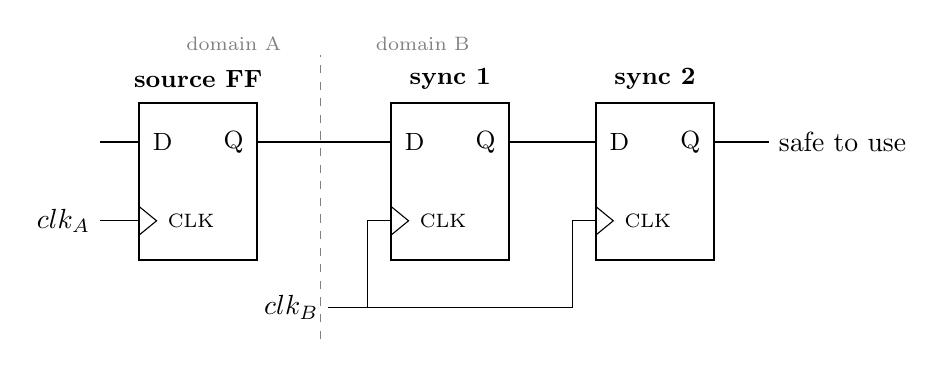
\begin{tikzpicture}
  \dbox{s}{(0,0)}{source FF}{1}
  \dbox{a}{(3.2,0)}{sync 1}{1}
  \dbox{b}{(5.8,0)}{sync 2}{1}
  \draw (s-q) -- (a-d); \draw (a-q) -- (b-d);
  \draw (b-q) -- ++(0.7,0) node[right]{safe to use};
  \draw (s-d) -- ++(-0.5,0);
  \draw (s-clk) -- ++(-0.5,0) node[left]{$clk_A$};
  \draw (a-clk) -- ++(-0.3,0) |- (3.0,-0.6) -- (5.5,-0.6) |- (b-clk);
  \draw (3.0,-0.6) -- ++(-0.6,0) node[left]{$clk_B$};
  \draw[dashed,gray] (2.3,-1.0) -- (2.3,2.6);
  \node[font=\scriptsize,gray] at (1.2,2.75) {domain A};
  \node[font=\scriptsize,gray] at (3.6,2.75) {domain B};
\end{tikzpicture}
\caption{A two-flop synchronizer. The signal leaves domain A from a flip-flop (never from raw logic) and is re-timed by two flip-flops on clock B.}
\label{fig:sync}
\end{figure}

Rules that go with it:
\begin{itemize}
  \item The signal must come straight from a flip-flop in the source domain, not from combinational logic, which could glitch.
  \item A short pulse from a fast domain may fall entirely between the slow domain's clock edges and be missed. Stretch it, or convert it into a level that toggles (a ``toggle synchronizer'').
\end{itemize}

\paragraph{Many bits: never synchronize each bit separately.} If a multi-bit value changes, its bits pass through separate synchronizers with slightly different delays, and the receiver can see a mixture of old and new bits, a value that never existed. Safe methods:
\begin{itemize}
  \item \textbf{Gray code}: if the value is a counter, encode it in Gray code (Section~\ref{sec:gray}). Only one bit changes per step, so the receiver sees either the old value or the new one, never garbage.
  \item \textbf{Handshake}: hold the data stable, send a single ``valid'' bit through a synchronizer, and wait for an acknowledgment to come back the same way before changing the data.
  \item \textbf{Asynchronous FIFO}: the general solution for streams of data, described next.
\end{itemize}

\section{FIFOs}

A \term{FIFO} (first in, first out) is a queue: data is written at one end and read out in the same order at the other. It decouples a producer and a consumer that run at different moments or rates.

\paragraph{Structure.} A FIFO is a small memory used as a circular buffer, plus a \term{write pointer} (where the next word goes) and a \term{read pointer} (where the next word comes from). Both advance and wrap around. The FIFO is \term{empty} when the pointers are equal and \term{full} when the write pointer has gone all the way around and caught up with the read pointer. To tell these two cases apart, the pointers get one extra bit: equal including the extra bit means empty; equal except for the extra bit means full.

\paragraph{Asynchronous FIFOs.} When the writer and reader use different clocks, each side must compare its own pointer with the other side's pointer, which crosses a clock domain. The pointers are converted to Gray code and passed through two-flop synchronizers. Because only one bit changes at a time, the synchronized pointer is always a valid (if slightly old) value, and a slightly old value can only make the FIFO look a little fuller or emptier than it is, which is safe.

\section{How deep must a FIFO be?}
\label{sec:fifodepth}

\begin{bigidea}
A FIFO must hold whatever the writer produces faster than the reader can consume. During a burst of $B$ words, the writer takes time $B/r_w$ (where $r_w$ is the write rate in words per second), and in that time the reader removes $r_r \cdot B/r_w$ words. The rest must wait in the FIFO:
\[
  \text{depth} \ge B - B\,\frac{r_r}{r_w} = B\left(1 - \frac{r_r}{r_w}\right).
\]
\end{bigidea}

\begin{worked}{a simple burst}
The writer runs at 100\,MHz and writes one word per cycle in bursts of 120 words. The reader runs at 50\,MHz and reads one word per cycle. Burst time: $120/100\,\text{MHz} = 1.2\,\mu$s. Words read in that time: $1.2\,\mu\text{s} \times 50\,\text{MHz} = 60$. Depth: $120 - 60 = 60$ words.
\end{worked}

\begin{worked}{idle cycles}
The writer runs at 200\,MHz and writes a burst of 100 words, one per cycle. The reader runs at 100\,MHz but can only accept one word every 2 cycles, an effective rate of 50 million words per second. Burst time: $100/200\,\text{MHz} = 0.5\,\mu$s. Words read: $0.5 \times 50 = 25$. Depth: $100 - 25 = 75$ words.
\end{worked}

Real questions add details: idle cycles on the write side (use the effective rate), a worst case where two bursts arrive back to back, or a few extra entries for synchronizer latency in an asynchronous FIFO. Always convert everything to \emph{words per second} first. If the reader is at least as fast as the writer, a FIFO only needs to cover latency, not rate mismatch.

\begin{onoa}
FIFOs are reported on the Ignite assessment, and FIFO depth calculations (module A writing to module B at a different frequency) on other NVIDIA hardware tests. Be ready to explain what a FIFO is, how full and empty are detected, why asynchronous FIFOs use Gray-coded pointers, and how to size one.
\end{onoa}

\section{Handshakes and arbiters}

\paragraph{Valid/ready.} Within one clock domain, blocks usually exchange data with a \term{valid/ready} handshake: the sender raises \code{valid} when it has data; the receiver raises \code{ready} when it can take it; a transfer happens on each clock edge where both are high. This lets either side pause the other (\term{backpressure}).

\paragraph{Arbiters.} When several requesters share one resource (a memory port, a bus), an \term{arbiter} grants it to one at a time. A \term{fixed-priority} arbiter always prefers the lowest-numbered requester, which is simple but can starve the others. A \term{round-robin} arbiter rotates priority after each grant, so every requester is eventually served.

\section{Verification basics}
\label{sec:verif}

Writing RTL is half the job. The other half, usually the larger half, is \term{verification}: showing that the RTL does what the specification says, in every situation it will meet, \emph{before} the chip is manufactured. A bug found in simulation costs an afternoon. A bug found in silicon can cost a new set of manufacturing masks (millions of dollars at advanced nodes) and months of delay, or a product recall. That is why large chip teams often have more verification engineers than designers, and why ``GPU Verification and Design'' is one of the Ignite internship areas.

\begin{bigidea}
Verification asks three questions, again and again: \textbf{Did I drive the design with enough different inputs?} (stimulus) \textbf{Did I check every output for the right answer?} (checking) \textbf{How do I know I have tested enough?} (coverage)
\end{bigidea}

\subsection*{The verification plan}

Before writing any test, a verification engineer reads the specification and writes a \term{verification plan}: a list of every feature and every rule the design must obey, how each will be tested, and what ``tested enough'' means for it. For a FIFO the plan would include: write then read returns the same data in order; \code{full} rises exactly when the FIFO holds \code{DEPTH} words; writing while full is ignored or flagged; reading while empty is ignored or flagged; simultaneous read and write work at every fill level; reset empties it.

\subsection*{Testbenches}

A \term{testbench} is a piece of HDL (or software) that surrounds the \term{design under test} (DUT), drives its inputs and watches its outputs. The testbench never becomes hardware, so it can use every language feature: loops, random numbers, files, classes.

\begin{figure}[h]
\centering
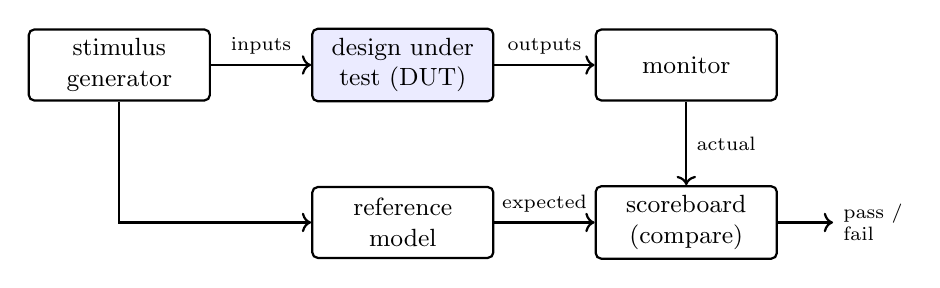
\begin{tikzpicture}[box/.style={draw,thick,rounded corners=2pt,minimum width=2.3cm,minimum height=0.9cm,font=\small,align=center}]
  \node[box] (gen) at (0,0) {stimulus\\generator};
  \node[box,fill=blue!8] (dut) at (3.6,0) {design under\\test (DUT)};
  \node[box] (mon) at (7.2,0) {monitor};
  \node[box] (sb) at (7.2,-2.0) {scoreboard\\(compare)};
  \node[box] (ref) at (3.6,-2.0) {reference\\model};
  \draw[->,thick] (gen) -- node[above,font=\scriptsize]{inputs} (dut);
  \draw[->,thick] (dut) -- node[above,font=\scriptsize]{outputs} (mon);
  \draw[->,thick] (mon) -- node[right,font=\scriptsize]{actual} (sb);
  \draw[->,thick] (gen.south) |- (ref.west);
  \draw[->,thick] (ref) -- node[above,font=\scriptsize]{expected} (sb);
  \draw[->,thick] (sb.east) -- ++(0.7,0) node[right,font=\scriptsize,align=left]{pass /\\fail};
\end{tikzpicture}
\caption{A self-checking testbench. The same stimulus goes to the design and to a reference model; a scoreboard compares what the design did with what it should have done.}
\label{fig:testbench}
\end{figure}

The most important rule: a testbench must \term{check} results automatically. Looking at waveforms by eye works for ten cycles, not for ten million. A \term{self-checking testbench} computes the expected answer itself, from a \term{reference model} (also called a \term{golden model}): a simple, obviously correct description of what the design should do, often written in SystemVerilog, C or Python. The reference model does not need to be fast or synthesizable, only right.

\begin{lstlisting}[language=Verilog]
module tb_adder8;
  logic [7:0] a, b;
  logic [8:0] sum;
  int errors = 0;

  adder8 dut (.a(a), .b(b), .sum(sum));   // the design under test

  task check(input logic [7:0] x, y);
    a = x; b = y;
    #1;                                   // let the logic settle
    if (sum !== x + y) begin              // reference model: the + operator
      errors++;
      $display("FAIL: %0d + %0d gave %0d", x, y, sum);
    end
  endtask

  initial begin
    check(8'd0,   8'd0);                  // directed corner cases first
    check(8'd255, 8'd1);
    check(8'd255, 8'd255);
    repeat (10000) check($urandom, $urandom);   // then random inputs
    $display("%0d errors", errors);
    $finish;
  end
endmodule
\end{lstlisting}

The comparison uses \code{!==}, which also catches \code{X} (unknown) and \code{Z} values on the output; \code{!=} would quietly treat them as ``not different.''

\subsection*{Directed, random and constrained-random tests}

\begin{itemize}
  \item A \term{directed test} applies inputs chosen by hand to exercise one feature or corner case: fill the FIFO exactly to full, add $255 + 1$. Directed tests are easy to understand, but they only find the bugs someone thought of.
  \item \term{Random} stimulus finds the bugs nobody thought of, but purely random inputs are often illegal (a packet length of zero, a misaligned address) or miss rare situations.
  \item \term{Constrained-random} stimulus is random within rules that keep it legal and steer it toward interesting cases. SystemVerilog builds this into the language:
\end{itemize}

\begin{lstlisting}[language=Verilog]
class packet;
  rand bit [7:0]  len;
  rand bit [31:0] addr;
  constraint legal { len inside {[1:64]};        // 1 to 64 bytes
                     addr[1:0] == 2'b00; }        // word-aligned
endclass
\end{lstlisting}

Each run uses a \term{seed} for its random number generator, and the seed is printed, so any failing run can be repeated exactly. Teams run \term{regressions}: thousands of tests with different seeds every night, so that a change that breaks something is caught the next morning.

\subsection*{Assertions}

An \term{assertion} states a rule that must always hold and reports an error the moment it is broken, at the place where the bug happens, not hundreds of cycles later when a wrong value finally reaches an output. SystemVerilog has two kinds:
\begin{itemize}
  \item An \term{immediate assertion} checks a condition at one moment, like an \code{if} that reports an error: \code{assert (count <= DEPTH);}
  \item A \term{concurrent assertion} (SystemVerilog Assertions, SVA) checks a property over clock cycles:
\end{itemize}

\begin{lstlisting}[language=Verilog]
// every request is granted within 1 to 3 cycles
assert property (@(posedge clk) disable iff (!rst_n) req |-> ##[1:3] gnt);

// the FIFO is never written while it is full
assert property (@(posedge clk) disable iff (!rst_n) !(wr_en && full));
\end{lstlisting}

Read \code{|->} as ``implies, starting this cycle'' and \code{\#\#[1:3]} as ``1 to 3 cycles later.'' Assertions are written once and then checked in every test, and formal tools (below) can try to prove them.

\subsection*{Coverage: how do you know you are done?}

Passing tests prove nothing about the situations the tests never reached. \term{Coverage} measures what was reached.
\begin{itemize}
  \item \term{Code coverage} is collected automatically by the simulator: which lines ran (line coverage), which branches of each \code{if} and \code{case} were taken (branch coverage), whether every signal toggled both ways (toggle coverage), and which FSM states and transitions occurred.
  \item \term{Functional coverage} is written by the engineer from the verification plan: did the scenarios that matter actually happen? Was the FIFO ever full? Was it written and read in the same cycle while full? Did every opcode run with a negative operand?
\end{itemize}

\begin{lstlisting}[language=Verilog]
covergroup fifo_cg @(posedge clk);
  level: coverpoint count { bins empty  = {0};
                            bins middle = {[1:DEPTH-1]};
                            bins full   = {DEPTH}; }
  ops:   cross wr_en, rd_en;       // all four write/read combinations
endgroup
\end{lstlisting}

\begin{trap}
100\% code coverage does not mean the design is correct. It means every line \emph{ran}, not that its results were \emph{checked}, and not that every combination of conditions occurred. A line can execute with the wrong answer in a test that has no checker. Coverage measures the stimulus; only checkers and assertions find bugs.
\end{trap}

Verification is ``done'' (\term{coverage closure}) when the plan's coverage goals are met, every test passes across many seeds, and the rate of newly found bugs has dropped to near zero.

\subsection*{Formal verification}

Simulation checks the input sequences you happen to try. \term{Formal verification} uses mathematical tools to prove that a property holds for \emph{every} possible input sequence (usually up to a bounded number of cycles), or to produce a counterexample: a short, exact input sequence that breaks it. It shines on control logic such as arbiters, FIFOs, handshakes and cache-coherence rules, where rare interleavings hide bugs. \term{Equivalence checking} is a related formal technique that proves two versions of a design behave identically, for example the RTL and the gate-level netlist produced by synthesis.

\subsection*{UVM and the bigger picture}

The \term{Universal Verification Methodology} (UVM) is a standard SystemVerilog class library for building large, reusable testbenches. Its pieces map onto Figure~\ref{fig:testbench}: a \term{sequencer} produces transactions (such as ``write 4 bytes to address 0x40''), a \term{driver} turns them into pin wiggles, a \term{monitor} turns pin activity back into transactions, and these three form an \term{agent} for one interface. A \term{scoreboard} compares observed transactions with the reference model. An agent written once for a bus can be reused on every block that uses that bus.

Verification also happens at several levels. Each block is tested on its own (unit level), then blocks together (subsystem), then the whole chip. Gate-level simulation checks the synthesized netlist. Because full-chip simulation is slow, companies also map the design onto \term{emulators} and FPGA prototypes, which run thousands of times faster, so real software and drivers can run on the chip before it exists. Arithmetic units are a classic verification target: Chapter~\ref{ch:arith} describes the corner cases they are checked against.

\begin{remember}
A test without a checker tests nothing. Start every testbench with a reference model and an automatic comparison, add constrained-random stimulus and assertions, and measure functional coverage against a written plan.
\end{remember}

\section{Summary}

\begin{itemize}
  \item HDLs describe parallel hardware. \code{assign} and \code{always @(*)} make combinational logic; \code{always @(posedge clk)} makes flip-flops.
  \item Nonblocking \code{<=} updates all left sides together at the end of the step (use in clocked blocks). Blocking \code{=} updates immediately (use in combinational blocks).
  \item Missing assignments in combinational blocks infer latches.
  \item Asynchronous resets need synchronous release. A delay-and-combine filter rejects reset glitches shorter than the delay.
  \item Single bits cross clock domains through two-flop synchronizers; multi-bit values need Gray code, handshakes or asynchronous FIFOs.
  \item FIFO depth $\ge B(1 - r_r/r_w)$, with rates in words per second.
  \item Verification: a self-checking testbench compares the design against a reference model. Directed tests hit known corner cases; constrained-random tests find the unexpected. Assertions catch rule violations where they happen. Code coverage shows what ran; functional coverage shows which planned scenarios occurred; neither replaces checking. Formal tools prove properties for all inputs.
\end{itemize}

\section{Exercises}

\begin{enumerate}
  \item With \code{a = 3} and \code{b = 7}, what are \code{a} and \code{b} after one clock edge of \code{a = b; b = a;} (blocking)? Of \code{a <= b; b <= a;}?
  \item In the \code{\$display} example of Section~\ref{sec:blocking}, what is printed at the third clock edge?
  \item Will this infer a latch? \code{always @(*) case (sel) 2'b00: y = a; 2'b01: y = b; endcase} How would you fix it?
  \item Why do we use two flip-flops to synchronize a single bit? Why is this not enough for an 8-bit bus?
  \item A writer at 150\,MHz sends bursts of 300 words; a reader at 100\,MHz reads one word per cycle. What FIFO depth is needed?
  \item Why are asynchronous FIFO pointers passed between domains in Gray code?
  \item Glitches up to 15\,ns must be removed from a reset line using 2\,ns buffers. How many buffers are needed?
  \item Give one advantage of a synchronous reset and one of an asynchronous reset.
  \item Write a Verilog module for a 4-bit counter with enable and synchronous active-high reset.
  \item What makes a testbench ``self-checking''? What is a reference model?
  \item Give one strength of directed tests and one of constrained-random tests.
  \item What is the difference between an immediate and a concurrent assertion? Write a concurrent assertion that \code{gnt} is never high unless \code{req} is high in the same cycle.
  \item A block reaches 100\% line coverage. Name two kinds of bug that could still be present.
  \item What can formal verification show that simulation cannot?
\end{enumerate}

\subsection*{Answers}
\begin{enumerate}
  \item Blocking: \code{a = 7}, \code{b = 7}. Nonblocking: \code{a = 7}, \code{b = 3}.
  \item The values have swapped back by then: after two edges \code{a = 1, b = 2}, so the third edge prints \code{a=1 b=2}.
  \item Yes: for \code{sel} values 10 and 11, \code{y} is not assigned, so it must hold its value. Add \code{default: y = 0;} (or assign \code{y} a default before the \code{case}).
  \item The first flip-flop may go metastable; the second gives it a full cycle to resolve, making failures extremely rare. For a bus, the bits may be captured on different cycles, giving a mixed value that never existed.
  \item Burst time $= 300/150\,\text{MHz} = 2\,\mu$s; read in that time $= 200$; depth $= 100$.
  \item Only one bit changes per increment, so a pointer sampled mid-change is either the old or the new value, never a wrong one.
  \item $k \times 2 > 15$, so 8 buffers (16\,ns).
  \item Synchronous: no timing surprises; filtered by the clock. Asynchronous: works without a running clock and acts immediately.
  \item For example:
\begin{lstlisting}[language=Verilog]
module counter4 (input wire clk, rst, en, output reg [3:0] q);
  always @(posedge clk) begin
    if (rst)      q <= 4'd0;
    else if (en)  q <= q + 4'd1;
  end
endmodule
\end{lstlisting}
  \item It computes the expected result itself and compares it with the design's output automatically, reporting any mismatch. A reference model is a simple, trusted description of the correct behaviour (in SystemVerilog, C or Python) that produces those expected results.
  \item Directed: hits a specific corner case on purpose and is easy to debug. Constrained-random: explores many legal combinations nobody thought to write, finding unexpected bugs.
  \item An immediate assertion checks a condition at one instant, like an \code{if}; a concurrent assertion checks a property across clock cycles. For example: \code{assert property (@(posedge clk) gnt |-> req);}
  \item Lines that ran but whose results were never checked (a wrong answer nobody compared), and combinations of conditions that never occurred together (for example, a write and a read in the same cycle while full). Line coverage says nothing about either.
  \item That a property holds for \emph{every} possible input sequence (up to a bound), or an exact counterexample if it does not. Simulation only checks the sequences that were run.
\end{enumerate}

\chapter{Computer Architecture}
\label{ch:arch}

Computer architecture is the level above circuits: how a processor is organized to run programs quickly. Interviewers for hardware internships often ask about it (``what are the stages of a five-stage pipeline?''), and NVIDIA hardware tests have included cache and memory-timing calculations. This chapter gives the essentials.

\section{What a processor does}

A processor runs a program stored in memory as a list of \term{instructions}. The set of instructions a processor understands, and how they are encoded, is its \term{instruction set architecture} (ISA): x86 in most PCs, ARM in phones, RISC-V in many new designs. A processor holds a small number of fast \term{registers}, and a \term{program counter} (PC) that points at the next instruction. Each instruction goes through the same cycle:
\begin{enumerate}
  \item \textbf{Fetch} the instruction at the PC from memory.
  \item \textbf{Decode} it: what operation, which registers.
  \item \textbf{Execute}: do the arithmetic, compare, or compute an address.
  \item Access \textbf{memory} if it is a load or store.
  \item \textbf{Write back} the result to a register, and move the PC to the next instruction (or the branch target).
\end{enumerate}

Instructions come in a few families: arithmetic and logic (\code{add r1, r2, r3}), memory (\code{load r1, 8(r2)} and \code{store}), and control flow (\code{branch if equal}, \code{jump}).

\section{Measuring performance}

\begin{bigidea}
The \textbf{processor performance equation}:
\[
  \text{execution time} = \text{instruction count} \times \text{CPI} \times \text{clock period},
\]
where CPI is the average number of clock cycles per instruction. Every architecture idea attacks one of these three factors.
\end{bigidea}

\begin{worked}{run time}
A program executes $10^9$ instructions with an average CPI of 1.5 on a 2\,GHz processor (0.5\,ns period). Time $= 10^9 \times 1.5 \times 0.5\times10^{-9} = 0.75$\,s.
\end{worked}

\section{The five-stage pipeline}

A simple processor could do all five steps of one instruction in one long clock cycle. A \term{pipelined} processor instead splits the steps into stages separated by registers (Section~\ref{sec:pipelining}), and works on five different instructions at once, one in each stage, like an assembly line.

\begin{onoa}
``What are the stages in a five-stage pipelined processor?'' is a reported NVIDIA hardware intern interview question. The classic answer: \textbf{IF} (instruction fetch), \textbf{ID} (instruction decode and register read), \textbf{EX} (execute, using the ALU), \textbf{MEM} (memory access for loads and stores), \textbf{WB} (write back to the register file).
\end{onoa}

\begin{figure}[h]
\centering
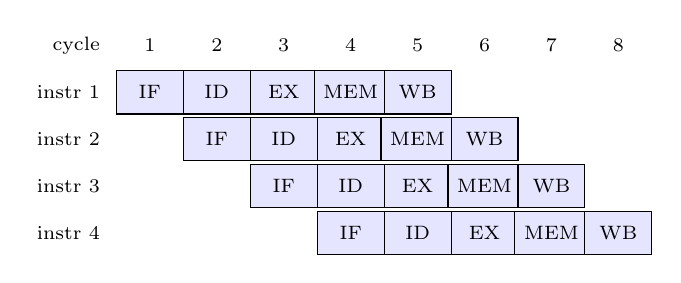
\begin{tikzpicture}[scale=0.85, st/.style={draw,minimum width=0.85cm,minimum height=0.55cm,font=\scriptsize}]
  \foreach \c in {1,...,8} \node[font=\scriptsize] at (\c,0.7) {\c};
  \node[font=\scriptsize,anchor=east] at (0.4,0.7) {cycle};
  \foreach \i/\name in {0/{instr 1},1/{instr 2},2/{instr 3},3/{instr 4}} {
    \node[font=\scriptsize,anchor=east] at (0.4,-\i*0.7) {\name};
    \foreach \s [count=\k from 0] in {IF,ID,EX,MEM,WB}
      \node[st,fill=blue!10] at (\i+\k+1,-\i*0.7) {\s};
  }
\end{tikzpicture}
\caption{A five-stage pipeline. Once full, one instruction finishes every cycle, even though each takes five cycles.}
\label{fig:pipeline}
\end{figure}

Each instruction still takes five cycles (its latency), but a new one finishes every cycle (the throughput), so the ideal CPI is 1 and the clock can be about five times faster than a single-cycle design.

\begin{worked}{pipeline speedup}
A non-pipelined processor runs at 2.5\,GHz but needs 5 cycles per instruction (CPI = 5). A pipelined version runs at 2\,GHz (pipeline registers add overhead) with CPI = 1.

Non-pipelined: $2.5\times10^9/5 = 0.5$ billion instructions per second. Pipelined: $2\times10^9/1 = 2$ billion. Throughput speedup: $2/0.5 = 4\times$.
\end{worked}

\section{Hazards}

Overlapping instructions causes three kinds of trouble, called \term{hazards}.

\paragraph{Structural hazards.} Two instructions need the same hardware in the same cycle (for example, one memory port for both fetching and loading). Fixed by duplicating hardware, such as separate instruction and data caches.

\paragraph{Data hazards.} An instruction needs a result that an earlier instruction has not yet written back:
\begin{lstlisting}
add r1, r2, r3     # r1 is written in WB (cycle 5)
sub r4, r1, r5     # but sub reads r1 in ID (cycle 3)
\end{lstlisting}
The fix is \term{forwarding} (or bypassing): send the result straight from the end of the EX stage to the input of the next instruction's EX stage, without waiting for write-back. Forwarding fixes most data hazards with no delay.

One case it cannot fully fix is the \term{load-use hazard}: a load's data only arrives at the end of MEM, too late for an instruction right behind it that needs it in EX. The pipeline must \term{stall} (insert a bubble) for one cycle. Compilers reorder instructions to put something useful in that slot.

\paragraph{Control hazards.} After a branch, the processor does not know which instruction comes next until the branch is resolved, but the pipeline keeps fetching. If it guessed wrong, the wrongly fetched instructions must be \term{flushed}, wasting cycles (the \term{branch penalty}). \term{Branch prediction} guesses the outcome: simple predictors remember each branch's recent behavior (for example with 2-bit saturating counters), and a branch target buffer remembers where it jumps. Modern predictors are right well over 90\% of the time.

\section{Amdahl's law}

Speeding up one part of a task only helps as much as that part matters. If a fraction $p$ of the work is sped up by a factor $s$:
\[
  \boxed{\text{overall speedup} = \frac{1}{(1 - p) + p/s}}
\]

\begin{worked}{parallel speedup}
80\% of a program can run in parallel on 16 cores. Speedup $= 1/(0.2 + 0.8/16) = 1/0.25 = 4$. Even with infinitely many cores, the speedup can never exceed $1/0.2 = 5$: the serial 20\% sets the ceiling.
\end{worked}

\section{The memory hierarchy}

Processors are far faster than DRAM. Waiting about 100\,ns for every memory access would waste hundreds of clock cycles each time. The solution is a hierarchy of memories, small and fast near the processor, large and slow further away:

\begin{center}
\begin{tabular}{lll}
\toprule
Level & Typical size & Typical access time (approximate) \\
\midrule
Registers & hundreds of bytes to kilobytes & under 1\,ns \\
L1 cache (SRAM) & tens of KB & about 1\,ns \\
L2 cache & hundreds of KB to a few MB & a few ns \\
L3 / last-level cache & many MB & 10--40\,ns \\
DRAM & gigabytes & 50--100\,ns \\
SSD (flash) & terabytes & about 100\,$\mu$s \\
\bottomrule
\end{tabular}
\end{center}

This works because programs have \term{locality}:
\begin{itemize}
  \item \textbf{Temporal locality}: data used recently is likely to be used again soon (loop variables).
  \item \textbf{Spatial locality}: data near recently used data is likely to be used soon (array elements in order).
\end{itemize}

\section{How a cache works}

A cache stores copies of recently used memory in fixed-size blocks called \term{lines} (often 64 bytes; fetching a whole line exploits spatial locality). To find whether an address is in the cache, the address is split into three fields:
\[
  \underbrace{\text{tag}}_{\text{which line is this?}} \;\big|\; \underbrace{\text{index}}_{\text{which set to look in}} \;\big|\; \underbrace{\text{offset}}_{\text{which byte in the line}}
\]
\begin{itemize}
  \item \textbf{Offset} bits $= \log_2(\text{line size})$.
  \item \textbf{Index} bits $= \log_2(\text{number of sets})$.
  \item \textbf{Tag} bits $=$ address bits $-$ index bits $-$ offset bits. Each line stores its tag so the cache can check whether it holds the right address, plus a \term{valid} bit and usually a \term{dirty} bit.
\end{itemize}

\paragraph{Associativity.} In a \term{direct-mapped} cache, each address can go in exactly one line. In an \term{$N$-way set-associative} cache, each address maps to one \emph{set} of $N$ lines and can go in any of them. In a \term{fully associative} cache, it can go anywhere. More associativity means fewer conflicts but more tags to compare in parallel. When a set is full, a \term{replacement policy} (usually least recently used, LRU, or an approximation) picks a line to evict.

\paragraph{Writes.} A \term{write-through} cache sends every write on to the next level immediately. A \term{write-back} cache only updates its own copy and marks the line \emph{dirty}, writing it back when it is evicted, which saves bandwidth.

\paragraph{Why misses happen (the three Cs).} \textbf{Compulsory} misses: the first access to a line. \textbf{Capacity} misses: the working data does not fit. \textbf{Conflict} misses: too many addresses map to the same set, even though the cache has room elsewhere (eliminated by full associativity).

\begin{worked}{address fields and tag-array size}
A 1\,MB, 4-way set-associative cache has 64-byte lines and 32-bit addresses. Each line stores its tag plus a valid bit and a dirty bit. How big is the tag array?

Lines: $2^{20}/2^6 = 2^{14} = 16{,}384$. Sets: $16{,}384/4 = 4096 = 2^{12}$.
Offset: 6 bits. Index: 12 bits. Tag: $32 - 12 - 6 = 14$ bits.
Bits per line: $14 + 1 + 1 = 16$. Tag array: $16{,}384 \times 16 = 262{,}144$ bits $= 32$\,KB.
\end{worked}

\section{Average memory access time}

\begin{bigidea}
\[
  \text{AMAT} = \text{hit time} + \text{miss rate} \times \text{miss penalty}.
\]
With two levels, the L1 miss penalty is itself the AMAT of L2:
\[
  \text{AMAT} = t_{L1} + m_{L1}\,\big(t_{L2} + m_{L2}\,t_{mem}\big),
\]
where $m_{L2}$ is the \emph{local} miss rate of L2 (the fraction of L2 accesses that miss).
\end{bigidea}

\begin{worked}{a two-level AMAT}
L1 hits 80\% of the time and L2 hits 40\% of the accesses that reach it. Access times are 10\,ns for L1, 30\,ns for L2 and 100\,ns for memory.
\[
  \text{AMAT} = 10 + 0.2\,(30 + 0.6 \times 100) = 10 + 0.2 \times 90 = 28~\text{ns}.
\]
\end{worked}

\begin{trap}
Some questions state each level's time as the \emph{total} time for an access served at that level, not the extra time added on a miss. Then the answer is a weighted average of where accesses are served: $0.8 \times 10 + 0.2 \times 0.4 \times 30 + 0.2 \times 0.6 \times 100 = 8 + 2.4 + 12 = 22.4$\,ns. Read the wording to decide which model the question uses, and say which one you assumed.
\end{trap}

\begin{worked}{memory stalls and CPI}
A processor has a base CPI of 1.0. 30\% of instructions are loads or stores, their L1 miss rate is 2\%, and a miss costs 200 cycles. Memory stall cycles per instruction: $0.3 \times 0.02 \times 200 = 1.2$. Effective CPI: $1.0 + 1.2 = 2.2$. The memory system more than doubles the run time, which is why caches are worth so much silicon. To compare two memory systems (for example, L3 only versus L2 plus L3), compute the effective CPI for each and take the ratio.
\end{worked}

\section{Virtual memory}

Programs use \term{virtual addresses}; the hardware translates them to \term{physical addresses} in DRAM. Memory is divided into \term{pages}, typically 4\,KB. A per-process \term{page table} maps virtual page numbers to physical page numbers; the offset within the page (the low 12 bits for 4\,KB pages) is unchanged by translation. A \term{translation lookaside buffer} (TLB), a small cache of recent translations, makes this fast. Accessing a page that is not in memory causes a \term{page fault}, handled by the operating system.

This is why ``are two addresses on the same 4\,KB page?'' (Section~\ref{sec:bitops}) is a natural hardware question: same page means same translation.

\section{Endianness}

A 32-bit value occupies 4 bytes in memory. A \term{little-endian} machine (x86, most ARM and RISC-V systems) stores the least significant byte at the lowest address; a \term{big-endian} machine stores the most significant byte first. The value \code{0x12345678} stored at address \code{0x100}:
\begin{center}
\begin{tabular}{lcccc}
\toprule
Address & \code{0x100} & \code{0x101} & \code{0x102} & \code{0x103} \\
\midrule
Little-endian & \code{78} & \code{56} & \code{34} & \code{12} \\
Big-endian & \code{12} & \code{34} & \code{56} & \code{78} \\
\bottomrule
\end{tabular}
\end{center}

\section{Multiple cores}

A chip with several cores, each with its own cache, must keep the caches \term{coherent}: if one core writes a value, other cores must not keep reading a stale copy. Coherence protocols such as MESI track whether each cached line is Modified, Exclusive, Shared or Invalid, and invalidate other copies when one core writes.

\section{Summary}

\begin{itemize}
  \item Execution time $=$ instruction count $\times$ CPI $\times$ clock period.
  \item Five-stage pipeline: IF, ID, EX, MEM, WB. Ideal CPI of 1.
  \item Hazards: structural (duplicate hardware), data (forwarding; load-use needs a stall), control (branch prediction, flush).
  \item Amdahl: speedup $= 1/((1-p) + p/s)$; the serial part sets the limit.
  \item Caches exploit temporal and spatial locality. Address $=$ tag $|$ index $|$ offset.
  \item AMAT $=$ hit time $+$ miss rate $\times$ miss penalty, applied level by level.
  \item Virtual memory translates pages (4\,KB); the TLB caches translations.
  \item Little-endian stores the least significant byte first.
\end{itemize}

\section{Exercises}

\begin{enumerate}
  \item A program runs $2\times10^9$ instructions at CPI 1.2 on a 3\,GHz processor. How long does it take?
  \item Name the five stages of the classic pipeline and say what each does.
  \item Why does a load followed immediately by an instruction using its result need a stall, even with forwarding?
  \item 90\% of a task is parallel. What is the speedup on 10 cores? The maximum on unlimited cores?
  \item A 32\,KB direct-mapped cache has 64-byte lines and 32-bit addresses. Find the offset, index and tag widths.
  \item A cache has a 1\,ns hit time, 5\% miss rate and 100\,ns miss penalty. Find the AMAT.
  \item Which kind of miss does full associativity eliminate?
  \item Show how \code{0xA1B2C3D4} is stored at address 0 in a little-endian machine.
  \item Base CPI 1.0, 40\% loads/stores, 5\% miss rate, 100-cycle penalty. What is the effective CPI?
\end{enumerate}

\subsection*{Answers}
\begin{enumerate}
  \item $2\times10^9 \times 1.2 / (3\times10^9) = 0.8$\,s.
  \item IF fetches the instruction; ID decodes it and reads registers; EX computes in the ALU; MEM reads or writes data memory; WB writes the result to the register file.
  \item The loaded value is only available at the end of MEM, but the next instruction needs it at the start of its EX stage, which happens in the same cycle; it must wait one cycle.
  \item $1/(0.1 + 0.09) \approx 5.3$. Maximum $1/0.1 = 10$.
  \item Offset 6 bits; lines $= 2^{15}/2^6 = 512$, so index 9 bits; tag $32 - 9 - 6 = 17$ bits.
  \item $1 + 0.05 \times 100 = 6$\,ns.
  \item Conflict misses.
  \item Address 0: \code{D4}, 1: \code{C3}, 2: \code{B2}, 3: \code{A1}.
  \item $1.0 + 0.4 \times 0.05 \times 100 = 3.0$.
\end{enumerate}

\chapter{GPUs and Parallel Computing}
\label{ch:gpu}

NVIDIA builds GPUs, so it is worth understanding what makes a GPU different from a CPU and why it is so good at graphics and AI. This chapter ties together many earlier ideas: parallelism to save power (Chapter~\ref{ch:power}), memory bandwidth (Chapter~\ref{ch:wires}), caches (Chapter~\ref{ch:arch}) and number formats (Chapter~\ref{ch:binary}). The Ignite posting lists familiarity with GPU programming (CUDA or OpenCL) as a plus.

\section{Two philosophies: latency and throughput}

A \textbf{CPU} is designed to finish \emph{one} thread of instructions as fast as possible. It spends its transistors on large caches, branch prediction, and complex out-of-order logic that finds independent instructions to run early. It has a handful of powerful cores.

A \textbf{GPU} is designed to finish a \emph{huge number} of similar, independent tasks at the greatest total rate. It spends its transistors on thousands of simple arithmetic units, and it tolerates slow memory not by avoiding waits but by always having other work ready.

\begin{everyday}
A CPU is a few expert chefs who can cook any dish quickly. A GPU is a giant kitchen with thousands of line cooks, each doing the same simple step on a different plate. For one complicated dish, the expert wins. For ten thousand identical burgers, the kitchen wins by a mile.
\end{everyday}

Graphics and AI are full of identical, independent work: every pixel on the screen, every element of a large matrix multiplication. That is why GPUs excel at both.

\section{How a GPU is organized}

\begin{itemize}
  \item The chip contains many \term{streaming multiprocessors} (SMs). Each SM has many arithmetic units (``CUDA cores''), special units for matrix math (tensor cores), a very large \term{register file}, and a fast on-chip SRAM called \term{shared memory} (configurable together with the L1 cache).
  \item All SMs share a large \term{L2 cache}, which connects to high-bandwidth DRAM (HBM or GDDR) through very wide memory interfaces.
  \item Threads are grouped into \term{warps} of 32 threads. All 32 threads of a warp execute the same instruction at the same time, each on its own data. NVIDIA calls this \term{SIMT}: single instruction, multiple threads.
\end{itemize}

\section{Hiding latency with many threads}

A memory access to DRAM takes hundreds of cycles. A CPU tries to avoid that wait with big caches and prediction. A GPU instead keeps many warps resident on each SM, with all of their registers held in the large register file. When one warp stalls waiting for memory, the warp scheduler simply issues an instruction from another warp that is ready, with no cost to switch. As long as there are enough ready warps, the arithmetic units stay busy. The fraction of the maximum possible warps actually resident on an SM is called \term{occupancy}.

\section{Two performance pitfalls}

\paragraph{Divergence.} The 32 threads of a warp share one instruction stream. If an \code{if} statement sends some threads one way and others the other way, the warp must execute \emph{both} paths, one after the other, with the inactive threads masked off. In the worst case, half the threads are idle for each path, halving throughput. GPU code is fastest when threads in a warp follow the same path.

\paragraph{Uncoalesced memory access.} When the 32 threads of a warp read memory, the hardware combines (\term{coalesces}) their requests into as few wide memory transactions as possible. If thread $i$ reads element $i$ of an array, the 32 reads fall into a few consecutive lines: perfectly coalesced. If each thread reads an element far from its neighbors' (a large stride), every thread may need its own transaction, wasting most of the bandwidth.

\section{The CUDA programming model}

In CUDA, the programmer writes a \term{kernel}: a function that one thread runs. The kernel is launched on a \term{grid} of \term{thread blocks}, each block containing many threads (up to 1024). Blocks are assigned to SMs; threads within a block can cooperate through shared memory and synchronize with \code{\_\_syncthreads()}. Each thread finds its own piece of work from its indices.

\begin{lstlisting}[language=C]
// Each thread adds one pair of elements: c[i] = a[i] + b[i]
__global__ void vec_add(const float *a, const float *b, float *c, int n) {
    int i = blockIdx.x * blockDim.x + threadIdx.x;   // global thread index
    if (i < n)                                       // guard the last block
        c[i] = a[i] + b[i];
}

// Launch enough blocks of 256 threads to cover n elements:
// vec_add<<<(n + 255) / 256, 256>>>(a, b, c, n);
\end{lstlisting}

Consecutive threads touch consecutive elements, so the accesses are coalesced, and there is no divergence except in the final partial block.

\section{Matrix multiplication and tensor cores}

Neural networks spend most of their time multiplying matrices. Multiplying an $M \times K$ matrix by a $K \times N$ matrix takes $M N K$ multiply-adds, which is $2MNK$ floating-point operations (FLOPs).

\begin{worked}{counting FLOPs}
Multiplying two $4096 \times 4096$ matrices takes $2 \times 4096^3 \approx 1.37\times10^{11}$ FLOPs. A GPU sustaining 500 TFLOP/s ($5\times10^{14}$ per second) does it in about 0.27\,ms.
\end{worked}

\term{Tensor cores} are hardware units that compute a whole small matrix multiply-and-add ($D = A \times B + C$ on small tiles) in one instruction, often using reduced-precision inputs. They deliver many times the throughput of ordinary arithmetic units for this one operation, which is why they dominate AI performance.

\section{Number formats}

\paragraph{Floating point.} A floating-point number is stored as a sign bit $s$, an exponent $e$ and a fraction (mantissa) $m$, and represents
\[
  (-1)^s \times 1.m \times 2^{\,e - \text{bias}}.
\]
For 32-bit IEEE floating point (FP32), the exponent has 8 bits with a bias of 127, and the fraction has 23 bits. The exponent sets the \emph{range} (how large or small a number can be); the fraction sets the \emph{precision} (how many significant digits).

\begin{worked}{decoding an FP32 number}
\code{0x40400000} $= 0\;10000000\;10000000000000000000000_2$. Sign 0 (positive). Exponent $128 - 127 = 1$. Fraction $.1_2 = 0.5$, so $1.m = 1.5$. Value: $1.5 \times 2^1 = 3.0$. Likewise \code{0x3F800000} is $1.0$, and \code{0xC0000000} is $-2.0$.
\end{worked}

Special patterns represent zero, infinity and NaN (``not a number,'' for results like $0/0$).

\begin{center}
\begin{tabular}{lcccl}
\toprule
Format & Sign & Exponent & Fraction & Notes \\
\midrule
FP32 & 1 & 8 & 23 & standard single precision \\
FP16 & 1 & 5 & 10 & half precision; smaller range \\
BF16 & 1 & 8 & 7 & same range as FP32, less precision \\
FP8 (E4M3) & 1 & 4 & 3 & more precision, less range \\
FP8 (E5M2) & 1 & 5 & 2 & more range, less precision \\
INT8 & \multicolumn{3}{c}{8-bit two's complement integer} & used with a scale factor \\
\bottomrule
\end{tabular}
\end{center}

Smaller formats move half or a quarter of the bytes and let each multiplier be much smaller, so throughput and energy efficiency rise sharply. AI training and inference tolerate reduced precision well, which is why GPUs keep adding smaller formats. \textbf{BF16} keeps FP32's 8-bit exponent, so it covers the same range of values and rarely overflows, at the cost of precision.

\section{Compute-bound or memory-bound?}

Every computation needs both arithmetic and data. Its \term{arithmetic intensity} is the number of FLOPs it performs per byte moved from memory. A GPU with peak compute $P$ (FLOP/s) and memory bandwidth $B$ (bytes/s) is balanced at an intensity of $P/B$:
\begin{itemize}
  \item below that, the program is \term{memory-bound}: the arithmetic units wait for data;
  \item above it, the program is \term{compute-bound}.
\end{itemize}
Plotting achievable performance against intensity gives the \term{roofline model}.

\begin{worked}{is vector add compute-bound?}
A GPU delivers 100 TFLOP/s and 2\,TB/s, so it balances at $100\times10^{12}/2\times10^{12} = 50$ FLOP per byte. Vector add (\code{c[i] = a[i] + b[i]} in FP32) does 1 FLOP per 12 bytes (two 4-byte loads and one 4-byte store): about 0.08 FLOP/byte, far below 50. It is heavily memory-bound; only bandwidth matters. A large matrix multiply reuses each loaded value many times, reaching high intensity, so it can use the full compute.
\end{worked}

This is why GPUs need enormous memory bandwidth (HBM, Chapter~\ref{ch:memory}) and why so much GPU programming is about reusing data held in registers and shared memory.

\section{Summary}

\begin{itemize}
  \item CPUs optimize latency for a few threads; GPUs optimize throughput for many.
  \item GPUs are built from SMs; threads run in warps of 32 under SIMT.
  \item GPUs hide memory latency by switching among many resident warps.
  \item Divergence serializes branches within a warp; uncoalesced accesses waste bandwidth.
  \item CUDA: a kernel runs per thread, over a grid of blocks; index $=$ \code{blockIdx.x * blockDim.x + threadIdx.x}.
  \item Matrix multiply $= 2MNK$ FLOPs; tensor cores accelerate it.
  \item Floating point $= (-1)^s \times 1.m \times 2^{e-\text{bias}}$; exponent bits set range, fraction bits set precision. BF16 has FP32's range.
  \item Arithmetic intensity versus the GPU's FLOP/byte balance decides compute-bound or memory-bound.
\end{itemize}

\section{Exercises}

\begin{enumerate}
  \item In one sentence each, what is a CPU optimized for and what is a GPU optimized for?
  \item How many threads are in a warp? What does SIMT mean?
  \item Half the threads of a warp take the \code{if} branch and half take the \code{else}. Roughly what fraction of the warp's peak throughput is achieved during that code?
  \item Thread $i$ reads \code{a[i * 64]} (4-byte floats). Is this coalesced? Why or why not?
  \item How many FLOPs does a $1024 \times 1024$ by $1024 \times 1024$ matrix multiply take?
  \item What is the arithmetic intensity of \code{y[i] = a * x[i] + y[i]} in FP32? Is it compute-bound or memory-bound on a typical GPU?
  \item Decode the FP32 bit pattern \code{0x40400000}.
  \item What does BF16 keep from FP32, and what does it give up?
  \item How are the 8 bits of FP8 E4M3 divided?
\end{enumerate}

\subsection*{Answers}
\begin{enumerate}
  \item A CPU minimizes the time to finish a single thread (latency); a GPU maximizes the total amount of parallel work finished per second (throughput).
  \item 32. One instruction is issued for all threads of a warp, each thread applying it to its own data.
  \item About half: the warp runs both paths one after the other, with half the threads idle in each.
  \item No. Consecutive threads are 256 bytes apart, so each thread's access falls in a different memory line, requiring many separate transactions.
  \item $2 \times 1024^3 \approx 2.15\times10^9$.
  \item 2 FLOPs (a multiply and an add) per 12 bytes (load $x$, load $y$, store $y$): about 0.17 FLOP/byte. Memory-bound.
  \item $3.0$ (sign 0, exponent $128 - 127 = 1$, significand 1.5).
  \item It keeps FP32's 8-bit exponent, and therefore its range. It gives up precision: 7 fraction bits instead of 23.
  \item 1 sign bit, 4 exponent bits, 3 fraction (mantissa) bits.
\end{enumerate}

\chapter{Computer Arithmetic: How Hardware Does Math}
\label{ch:arith}

A GPU is, more than anything, a machine for doing arithmetic: thousands of adders and multipliers working at once. NVIDIA's Ignite posting lists \emph{computer arithmetic} by name as a way to stand out. Chapter~\ref{ch:binary} showed how numbers are stored as bits, Chapter~\ref{ch:comb} built an adder, and Chapter~\ref{ch:gpu} introduced floating-point formats. This chapter puts those pieces to work: what happens when a result does not fit, how hardware shifts, adds quickly, multiplies and divides, how fractions are stored as fixed-point numbers, and how a floating-point unit actually adds and multiplies.

\begin{bigidea}
Every arithmetic circuit is a trade between three things: \textbf{speed} (how many gate delays from input to output), \textbf{area and power} (how many gates), and \textbf{accuracy} (how many bits, and how results are rounded). Faster adders and multipliers spend extra gates; smaller number formats save gates and energy by giving up precision.
\end{bigidea}

\section{When a result does not fit: carry, overflow and saturation}
\label{sec:overflow}

An $n$-bit adder always produces an $n$-bit result, plus a carry out of the top bit. The \emph{same} adder works for unsigned and for two's-complement signed numbers (Section~\ref{sec:twos}); only the meaning of ``the result did not fit'' differs.

\paragraph{Unsigned overflow: the carry.} For unsigned numbers, the result is too big exactly when there is a \term{carry out} of the most significant bit (MSB). In 8 bits, $200 + 100 = 300$, which does not fit in 0--255: the adder produces $300 - 256 = 44$ and a carry of 1.

\paragraph{Signed overflow: the overflow flag.} For signed numbers, the carry out means nothing on its own. Signed overflow happens when two numbers of the same sign produce a result of the opposite sign. Hardware detects it with one XOR gate:
\[
  V = c_{\text{into MSB}} \oplus c_{\text{out of MSB}}.
\]
If a carry goes into the sign bit but none comes out (or the reverse), the sign bit has been corrupted.

\begin{worked}{the four flags}
Add $0110\,0100$ (100) and $0011\,0010$ (50) in 8 bits. The result is $1001\,0110$.
\begin{itemize}
  \item As unsigned numbers: $100 + 50 = 150$, which fits in 0--255. There is no carry out, so $C = 0$, and $1001\,0110 = 150$ is correct.
  \item As signed numbers: $100 + 50 = 150$ does not fit in $-128$ to $127$. The result reads as $-106$. Bit 6 adds 1, 0 and an incoming carry, so a carry goes into the sign bit, but none comes out of it, so $V = 1$.
\end{itemize}
Processors record these as status \term{flags}: $C$ (carry), $V$ (overflow), $N$ (negative: the sign bit) and $Z$ (zero: every bit is 0). Here $C = 0$, $V = 1$, $N = 1$, $Z = 0$.
\end{worked}

\paragraph{Wrap or saturate?} When a result does not fit, ordinary integer hardware \term{wraps around}, keeping only the low $n$ bits. That is right for counters and addresses, but disastrous for a pixel brightness or an audio sample: a bright pixel that wraps becomes black. \term{Saturating arithmetic} instead clamps the result to the largest or smallest representable value.

\begin{center}
\begin{tabular}{lcc}
\toprule
8-bit operation & Wrapping result & Saturating result \\
\midrule
unsigned $200 + 100$ & 44 & 255 \\
unsigned $50 - 80$ & 226 & 0 \\
signed $100 + 50$ & $-106$ & 127 \\
signed $-100 - 50$ & 106 & $-128$ \\
\bottomrule
\end{tabular}
\end{center}

Saturation costs only a little logic: detect overflow ($C$ or $V$), and if it happened, select the maximum or minimum constant with a multiplexer instead of the adder's output. Digital signal processors, image pipelines and quantized neural-network hardware use it everywhere.

\begin{trap}
The carry flag is not the overflow flag. Adding $-1$ and $-1$ in 8 bits ($1111\,1111 + 1111\,1111$) produces a carry out, but the signed result $1111\,1110 = -2$ is perfectly correct, so $V = 0$.
\end{trap}

\section{Shifting}

\paragraph{Logical and arithmetic shifts.} Shifting left by $k$ multiplies by $2^k$ (if nothing falls off the top). Shifting right divides by $2^k$, and there are two kinds (Section~\ref{sec:bitops}): a \term{logical} right shift fills with zeros (for unsigned numbers), and an \term{arithmetic} right shift copies the sign bit in from the left, so negative numbers stay negative.

\begin{worked}{arithmetic shifts round down}
$-8$ in 8 bits is $1111\,1000$. Arithmetic right shift by 1: $1111\,1100 = -4$. Correct.

$-7$ is $1111\,1001$. Arithmetic right shift by 1: $1111\,1100 = -4$, not $-3$. An arithmetic shift rounds toward $-\infty$ (it computes $\lfloor -3.5 \rfloor = -4$), while integer division in C rounds toward zero ($-7/2 = -3$). Compilers add a small correction when they replace a signed division by a shift.
\end{worked}

\paragraph{The barrel shifter.} A processor must shift by any amount in a single cycle. A \term{barrel shifter} does it with $\log_2 n$ layers of 2:1 multiplexers. For a 32-bit value, the five bits of the shift amount control five layers that shift by 16, 8, 4, 2 and 1, each either shifting or passing the value straight through (Figure~\ref{fig:barrel}). Any amount from 0 to 31 is a sum of those powers of two. The cost: 5 layers of 32 multiplexers, 160 in all, but only five multiplexer delays.

\begin{figure}[h]
\centering
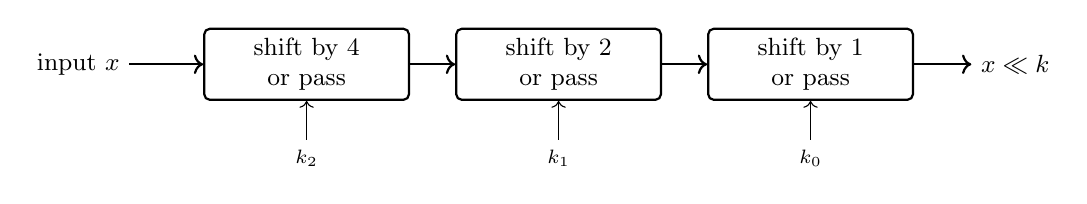
\begin{tikzpicture}[box/.style={draw,thick,rounded corners=2pt,minimum width=2.6cm,minimum height=0.8cm,font=\small,align=center}]
  \node[font=\small] (in) at (0,0) {input $x$};
  \node[box] (s4) at (2.9,0) {shift by 4\\or pass};
  \node[box] (s2) at (6.1,0) {shift by 2\\or pass};
  \node[box] (s1) at (9.3,0) {shift by 1\\or pass};
  \node[font=\small] (out) at (11.9,0) {$x \ll k$};
  \draw[->,thick] (in) -- (s4); \draw[->,thick] (s4) -- (s2); \draw[->,thick] (s2) -- (s1); \draw[->,thick] (s1) -- (out);
  \draw[<-] (s4.south) -- ++(0,-0.5) node[below,font=\scriptsize]{$k_2$};
  \draw[<-] (s2.south) -- ++(0,-0.5) node[below,font=\scriptsize]{$k_1$};
  \draw[<-] (s1.south) -- ++(0,-0.5) node[below,font=\scriptsize]{$k_0$};
\end{tikzpicture}
\caption{An 8-bit barrel shifter. Each layer is a row of 2:1 multiplexers controlled by one bit of the shift amount $k = k_2k_1k_0$. Shifting by 5 ($101_2$) means: shift by 4, pass, shift by 1.}
\label{fig:barrel}
\end{figure}

\paragraph{Multiplying by a constant.} Multiplying by a fixed number needs no multiplier at all, only shifts (which are free wiring) and adds:
\[
  10x = 8x + 2x = (x \ll 3) + (x \ll 1), \qquad 7x = 8x - x = (x \ll 3) - x.
\]
The second form uses a subtraction to replace two additions, the same trick Booth recoding uses below.

\section{Adding faster}
\label{sec:fastadd}

Chapter~\ref{ch:comb} built a ripple-carry adder: simple, but the carry may have to travel through every bit, so a 64-bit add takes 64 full-adder delays. Faster adders break that chain.

\paragraph{Generate and propagate.} For bit $i$, define
\begin{align*}
  G_i &= A_i B_i && \text{(this bit generates a carry: both bits are 1)}, \\
  P_i &= A_i \oplus B_i && \text{(this bit propagates an incoming carry: exactly one bit is 1)}.
\end{align*}
Then the carry out of bit $i$ is $c_{i+1} = G_i + P_i c_i$: a carry leaves bit $i$ if the bit makes one, or passes one along. Substituting each equation into the next gives every carry directly from the inputs:
\begin{align*}
  c_1 &= G_0 + P_0 c_0 \\
  c_2 &= G_1 + P_1 G_0 + P_1 P_0 c_0 \\
  c_3 &= G_2 + P_2 G_1 + P_2 P_1 G_0 + P_2 P_1 P_0 c_0 \\
  c_4 &= G_3 + P_3 G_2 + P_3 P_2 G_1 + P_3 P_2 P_1 G_0 + P_3 P_2 P_1 P_0 c_0
\end{align*}
Each line is just AND gates feeding an OR gate, so all four carries are ready after about two gate delays instead of four full-adder delays. This is a 4-bit \term{carry-lookahead adder} (CLA). The equations grow quickly, so wide adders apply the same idea in a tree: each 4-bit group computes a group generate and group propagate, and a second level of lookahead combines groups. \term{Prefix adders} (Kogge--Stone, Brent--Kung) are the systematic version, with delay growing as $\log_2 n$: about 6 levels for 64 bits instead of 64 stages.

\paragraph{Carry-select.} Compute the upper half of the sum twice, once assuming its carry-in is 0 and once assuming 1, while the lower half is still adding. When the real carry arrives, a multiplexer picks the right upper half. Speed for area: roughly double the adder hardware for the upper half.

\paragraph{Carry-save: adding three numbers without carrying.} A row of independent full adders takes three numbers and produces \emph{two}: a sum vector (each bit's $A \oplus B \oplus C$) and a carry vector (each bit's majority, shifted left one place). No carry travels sideways, so the delay is one full adder no matter how wide the numbers are. This \term{carry-save adder} (CSA), also called a 3:2 compressor, is the key to fast multipliers.

\begin{worked}{carry-save addition}
Add 5, 6 and 7 ($101$, $110$, $111$).
Sum vector: bitwise XOR of all three $= 100 = 4$.
Carry vector: bitwise majority $= 111$, shifted left $= 1110 = 14$.
One ordinary addition finishes the job: $4 + 14 = 18 = 5 + 6 + 7$. Reducing three numbers to two cost one full-adder delay; only the final addition needs a carry chain.
\end{worked}

\section{Multiplication}
\label{sec:mult}

\paragraph{Shift and add.} Binary multiplication is the long multiplication taught in school, but easier, because each digit of the multiplier is 0 or 1: each \term{partial product} is either zero or a shifted copy of the multiplicand.

\begin{worked}{$11 \times 13$ in binary}
\begin{center}
\begin{tabular}{rl}
\code{\ \ \ \ 1011} & multiplicand $= 11$ \\
$\times$\ \code{\ \ \ \ 1101} & multiplier $= 13$ \\
\midrule
\code{\ \ \ \ 1011} & bit 0 is 1: $11$ \\
\code{\ \ \ 0000\ } & bit 1 is 0: $0$ \\
\code{\ \ 1011\ \ } & bit 2 is 1: $11 \times 4 = 44$ \\
\code{\ 1011\ \ \ } & bit 3 is 1: $11 \times 8 = 88$ \\
\midrule
\code{10001111} & $11 + 44 + 88 = 143$ \\
\end{tabular}
\end{center}
Each partial-product bit is one AND gate (multiplicand bit AND multiplier bit). Multiplying an $n$-bit number by an $m$-bit number gives up to $n + m$ bits: here $4 + 4 = 8$, and indeed $15 \times 15 = 225$ needs all 8.
\end{worked}

\paragraph{Array multipliers and trees.} An $n \times n$ multiplier makes $n$ partial products from $n^2$ AND gates, then adds them up. An \term{array multiplier} adds them row by row in a grid of full adders: regular and easy to lay out, with delay that grows in proportion to $n$. A \term{Wallace tree} or \term{Dadda tree} instead feeds the partial products through layers of carry-save adders, each layer turning every three rows into two. The row count falls by about a third per layer, so $n$ rows shrink to two in about $\log_{1.5} n$ layers, and one fast adder from Section~\ref{sec:fastadd} produces the product. For 24 rows (an FP32 significand) that is 7 layers.

\paragraph{Booth recoding: fewer partial products.} Long runs of 1s are wasteful: $0111_2 = 7$ needs three partial products, but $7 = 8 - 1$ needs only two (a shifted copy and a subtracted copy). \term{Radix-4 Booth recoding} applies this systematically. It looks at the multiplier in overlapping groups of three bits $(b_{2i+1}, b_{2i}, b_{2i-1})$, with $b_{-1} = 0$, and turns each group into one digit:
\[
  d_i = -2\,b_{2i+1} + b_{2i} + b_{2i-1} \in \{-2, -1, 0, +1, +2\}.
\]
The multiplier then equals $\sum_i d_i \, 4^i$, so an $n$-bit multiplier needs only about $n/2$ partial products. Each is $0$, $\pm M$ or $\pm 2M$ (a shift), and negation is invert-plus-one, so they are cheap to make. Booth recoding also handles two's-complement (signed) multipliers with no special cases.

\begin{center}
\begin{tabular}{ccc|c|l}
\toprule
$b_{2i+1}$ & $b_{2i}$ & $b_{2i-1}$ & digit $d_i$ & partial product \\
\midrule
0 & 0 & 0 & $0$ & 0 \\
0 & 0 & 1 & $+1$ & $+M$ \\
0 & 1 & 0 & $+1$ & $+M$ \\
0 & 1 & 1 & $+2$ & $+2M$ (shift left) \\
1 & 0 & 0 & $-2$ & $-2M$ \\
1 & 0 & 1 & $-1$ & $-M$ \\
1 & 1 & 0 & $-1$ & $-M$ \\
1 & 1 & 1 & $0$ & 0 \\
\bottomrule
\end{tabular}
\end{center}

\begin{worked}{Booth-recoding 7}
The multiplier is $0111$, so $b_3 b_2 b_1 b_0 = 0111$ and $b_{-1} = 0$.
Group 0 is $(b_1, b_0, b_{-1}) = (1, 1, 0)$: $d_0 = -2 + 1 + 0 = -1$.
Group 1 is $(b_3, b_2, b_1) = (0, 1, 1)$: $d_1 = 0 + 1 + 1 = +2$.
Check: $d_1 \cdot 4 + d_0 = 8 - 1 = 7$. So $7M = 2M \cdot 4 - M$: two partial products instead of three.
\end{worked}

\paragraph{Why multipliers dominate AI hardware.} An $n \times n$ multiplier needs about $n^2$ partial-product bits, so its area and energy grow roughly with the \emph{square} of the width. An FP32 multiplier multiplies 24-bit significands; BF16 multiplies 8-bit ones (Chapter~\ref{ch:gpu}), so its multiplier is roughly $(24/8)^2 = 9$ times smaller. That, together with moving fewer bytes, is why tensor cores use narrow formats. A \term{multiply-accumulate} (MAC) unit, which computes $acc \leftarrow acc + a \times b$, is the building block of every tensor core and systolic array.

\section{Division}

Division is the slow operation. Binary long division produces \emph{one quotient bit per step}, and each step depends on the remainder from the previous one, so it cannot be done in parallel like a multiplier's partial products.

\paragraph{Restoring division.} Start with a remainder of 0. For each dividend bit, from the most significant down: shift the remainder left and bring in the next bit; if the remainder is now at least the divisor, subtract the divisor and write a quotient bit of 1, otherwise write 0. (The name comes from hardware that subtracts first and adds the divisor back, ``restoring,'' if the result went negative.)

\begin{worked}{$13 \div 3$}
Dividend $1101$, divisor $3$.
\begin{center}
\begin{tabular}{cccc}
\toprule
Bit brought in & Remainder & $\ge 3$? & Quotient bit \\
\midrule
1 & 1 & no & 0 \\
1 & $2 \cdot 1 + 1 = 3$ & yes, $3 - 3 = 0$ & 1 \\
0 & $2 \cdot 0 + 0 = 0$ & no & 0 \\
1 & $2 \cdot 0 + 1 = 1$ & no & 0 \\
\bottomrule
\end{tabular}
\end{center}
Quotient $0100 = 4$, remainder 1. Indeed $13 = 4 \times 3 + 1$.
\end{worked}

A 32-bit divide takes on the order of 32 steps. Faster dividers (SRT division) produce two or more quotient bits per step, and GPUs usually compute a reciprocal approximation from a small table and refine it with a couple of multiply-add iterations (Newton--Raphson), because multipliers are plentiful and fast.

\paragraph{Dividing by a constant.} Compilers and hardware avoid division by a known constant entirely: they multiply by a scaled reciprocal and shift. For any 16-bit unsigned $x$, $x / 3 = (x \times 43691) \gg 17$, because $43691 \approx 2^{17}/3$. A multiply and a shift replace a 16-step division.

\section{Fixed point: fractions on integer hardware}
\label{sec:fixed}

Integer hardware is small and fast, and many signals, such as audio samples, filter coefficients and neural-network weights, have a known, limited range. \term{Fixed-point} numbers store fractions in ordinary integers by agreeing on where the binary point is.

\begin{defn}{Q format}
A \textbf{Q$m$.$n$} number has $m$ integer bits and $n$ fraction bits. Its value is the stored integer divided by $2^n$. The \textbf{resolution} (the step between neighbouring values) is $2^{-n}$. For signed numbers, the sign is counted in $m$, so signed Q1.7 is 8 bits covering $-1$ to $1 - 2^{-7}$.
\end{defn}

\begin{worked}{reading and writing Q formats}
Unsigned Q4.4 pattern $0010\,1100$: integer part $0010 = 2$, fraction part $1100 = 12/16 = 0.75$, value 2.75. (Equivalently, $44 / 2^4 = 2.75$.)

Store 0.3 in signed Q1.7: $0.3 \times 2^7 = 38.4$, which rounds to 38. The stored value is $38/128 = 0.296875$, an error of about 0.003. The worst-case rounding error is half a step, $2^{-8} \approx 0.0039$.
\end{worked}

\paragraph{Arithmetic in fixed point.}
\begin{itemize}
  \item \textbf{Adding} needs both numbers in the same format, with their binary points lined up: shift one of them first if needed. Then it is a plain integer add (watch for overflow, and consider saturation).
  \item \textbf{Multiplying} two integers multiplies the scale factors too: a Q$a$.$b$ number times a Q$c$.$d$ number gives a Q$(a{+}c)$.$(b{+}d)$ product. To return to $b$ fraction bits, shift right by $d$, ideally rounding rather than truncating.
\end{itemize}

\begin{worked}{multiplying in Q1.7}
$0.5$ is stored as $64$ and $0.25$ as $32$ (both Q1.7). The integer product is $64 \times 32 = 2048$, a Q2.14 number. Shift right by 7: $2048 / 128 = 16$, which is $16/128 = 0.125$ in Q1.7. Correct: $0.5 \times 0.25 = 0.125$.
\end{worked}

\paragraph{Quantization for AI.} Neural-network inference often stores weights and activations as INT8 with a \term{scale factor} (and sometimes a zero point): $\text{real value} \approx s \times (q - z)$, where $q$ is the stored 8-bit integer. The scale is chosen per tensor or per channel so that the 256 available levels cover the values that actually occur. The multiply-adds run on cheap integer hardware with wide (32-bit) accumulators, and the result is rescaled at the end.

\section{Floating-point arithmetic}
\label{sec:fparith}

Chapter~\ref{ch:gpu} showed how a floating-point number is stored: sign $s$, exponent $e$ and fraction $m$, with value $(-1)^s \times 1.m \times 2^{e - 127}$ in FP32. Fixed point has a constant step size; floating point keeps a constant number of \emph{significant bits}, so it covers huge and tiny numbers alike. The cost is that every operation must line up exponents, renormalize and round.

\paragraph{Special values.} The smallest and largest exponent fields are reserved:
\begin{center}
\begin{tabular}{lll}
\toprule
Exponent field (FP32) & Fraction & Meaning \\
\midrule
1 to 254 & anything & normal number $1.m \times 2^{e-127}$ \\
0 & 0 & zero ($+0$ or $-0$) \\
0 & not 0 & subnormal number $0.m \times 2^{-126}$ \\
255 & 0 & $+\infty$ or $-\infty$ \\
255 & not 0 & NaN (not a number) \\
\bottomrule
\end{tabular}
\end{center}
Overflow gives $\pm\infty$; $1/0$ gives $+\infty$; $0/0$ and $\infty - \infty$ give NaN. NaN spreads through every later operation, and it is not equal to anything, not even itself.

\paragraph{Subnormal numbers.} The smallest normal FP32 number is $2^{-126} \approx 1.2\times10^{-38}$. Without subnormals, the next value down would be zero, and $x - y$ could be 0 even when $x \ne y$. \term{Subnormal} (denormal) numbers drop the hidden leading 1 to fill that gap evenly, down to $2^{-149} \approx 1.4\times10^{-45}$. This \term{gradual underflow} keeps small differences from vanishing. Handling subnormals takes extra hardware or time, so some processors offer \term{flush-to-zero} modes that replace them with 0 for speed; CUDA has such an option.

\paragraph{Precision.} With 23 stored fraction bits plus the hidden 1, FP32 has 24 significant bits. The gap between 1.0 and the next larger FP32 number is $2^{-23} \approx 1.2\times10^{-7}$ (\term{machine epsilon}), about 7 decimal digits of precision. The gap between neighbouring numbers is called a \term{ULP} (unit in the last place), and it grows with the number's size: between $2^{26}$ and $2^{27}$ the FP32 spacing is $2^{26-23} = 8$.

\subsection*{Floating-point addition}

\begin{figure}[h]
\centering
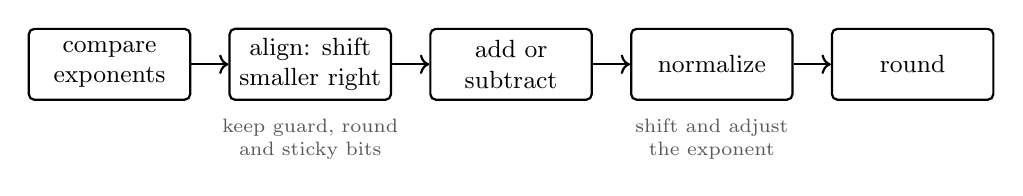
\begin{tikzpicture}[box/.style={draw,thick,rounded corners=2pt,minimum width=2.05cm,minimum height=0.9cm,font=\small,align=center}]
  \node[box] (a) at (0,0) {compare\\exponents};
  \node[box] (b) at (2.55,0) {align: shift\\smaller right};
  \node[box] (c) at (5.1,0) {add or\\subtract};
  \node[box] (d) at (7.65,0) {normalize};
  \node[box] (e) at (10.2,0) {round};
  \draw[->,thick] (a) -- (b); \draw[->,thick] (b) -- (c); \draw[->,thick] (c) -- (d); \draw[->,thick] (d) -- (e);
  \node[font=\scriptsize,gray!70!black,align=center] at (2.55,-0.95) {keep guard, round\\and sticky bits};
  \node[font=\scriptsize,gray!70!black,align=center] at (7.65,-0.95) {shift and adjust\\the exponent};
\end{tikzpicture}
\caption{The steps of a floating-point adder. Hardware pipelines these steps over several clock cycles.}
\label{fig:fpadd}
\end{figure}

\begin{enumerate}
  \item \textbf{Compare exponents.} The number with the smaller exponent must be adjusted to match the larger.
  \item \textbf{Align.} Shift the smaller number's significand right by the exponent difference.
  \item \textbf{Add or subtract} the significands (subtract if the signs differ).
  \item \textbf{Normalize.} Shift the result so it again has the form $1.xxx$, adjusting the exponent: one place right if the sum reached 2 or more, possibly many places left if a subtraction cancelled the leading bits.
  \item \textbf{Round} back to 23 fraction bits, and check for overflow, underflow and special values.
\end{enumerate}

\begin{worked}{$3.0 + 0.5$}
$3.0 = 1.1_2 \times 2^1$ and $0.5 = 1.0_2 \times 2^{-1}$. The exponents differ by 2, so shift the smaller significand right by 2: $1.0_2 \times 2^{-1} = 0.01_2 \times 2^1$. Add: $1.10_2 + 0.01_2 = 1.11_2$, so the result is $1.11_2 \times 2^1 = 3.5$. Already normalized; nothing to round.
\end{worked}

\paragraph{Guard, round and sticky bits.} During alignment, bits shifted off the right end are not simply thrown away. The adder keeps the first two of them (the \term{guard} and \term{round} bits) and ORs all the rest into one \term{sticky} bit (``was anything nonzero shifted out?''). Those three extra bits are exactly enough to round correctly, as if the exact result had been computed with infinite precision.

\subsection*{Floating-point multiplication}

Multiplication is simpler than addition because no alignment is needed:
\begin{enumerate}
  \item \textbf{Sign:} XOR of the two signs.
  \item \textbf{Exponent:} add the exponent fields and subtract one bias: $e = e_1 + e_2 - 127$.
  \item \textbf{Significand:} multiply the two 24-bit significands (a $24 \times 24$ integer multiplier, Section~\ref{sec:mult}). The product lies between 1 and 4.
  \item \textbf{Normalize} (shift right once if the product is 2 or more, and add 1 to the exponent), then \textbf{round}.
\end{enumerate}

\begin{worked}{$3.0 \times 2.5$}
$3.0 = 1.1_2 \times 2^1$ (exponent field 128) and $2.5 = 1.01_2 \times 2^1$ (exponent field 128). Sign: $0 \oplus 0 = 0$. Exponent field: $128 + 128 - 127 = 129$, meaning $2^2$. Significands: $1.1_2 \times 1.01_2 = 1.111_2$ (that is, $1.5 \times 1.25 = 1.875$). Result: $1.111_2 \times 2^2 = 7.5$. Correct.
\end{worked}

\subsection*{Rounding}

The exact result of an operation usually falls between two representable numbers, and the \term{rounding mode} picks one. IEEE 754 defines four:
\begin{itemize}
  \item \textbf{Round to nearest, ties to even} (the default): pick the nearer neighbour; on an exact tie, pick the one whose last bit is 0. In decimal terms, 2.5 rounds to 2 and 3.5 to 4. Always rounding ties upward would bias long sums upward; ties to even makes the errors cancel on average.
  \item \textbf{Toward zero} (truncation), \textbf{toward $+\infty$}, and \textbf{toward $-\infty$}: used for special purposes such as interval arithmetic.
\end{itemize}

\paragraph{Floating-point addition is not associative.} Because every operation rounds, the order of operations changes the result.

\begin{worked}{order matters}
In FP32, numbers near $10^8$ are spaced 8 apart ($10^8$ lies between $2^{26}$ and $2^{27}$). So $10^8 + 1$ rounds back to $10^8$, and
\[
  (10^8 + 1) - 10^8 = 0, \qquad\text{but}\qquad (10^8 - 10^8) + 1 = 1.
\]
A GPU that sums a million numbers in parallel adds them in a different order than a CPU loop does, so the two answers can differ in the last bits. Neither is ``wrong.'' This matters when verifying GPU arithmetic: results are compared within a tolerance, not bit for bit, unless the order is fixed.
\end{worked}

\paragraph{Fused multiply-add.} A \term{fused multiply-add} (FMA) computes $a \times b + c$ with a \emph{single} rounding at the end, instead of rounding the product and then the sum. It is both faster (one instruction) and more accurate. Modern GPUs and CPUs build their floating-point units around FMA, and a tensor core is essentially a block of multiply-adds.

\paragraph{Mixed precision.} AI hardware multiplies in a narrow format (FP16, BF16, FP8) but \emph{accumulates} in FP32. A long sum of small products in a narrow format would lose the small terms, exactly as in the $10^8 + 1$ example; a wide accumulator keeps them.

\section{How arithmetic hardware is checked}

An arithmetic unit has far too many inputs to test exhaustively (a 32-bit adder has $2^{64}$ input pairs). It is verified by comparing it against a \term{reference model}, a simple program that computes the right answer (Section~\ref{sec:verif}), using millions of random inputs plus the \term{corner cases} where bugs hide: zero, one, the largest and smallest values, values that overflow, and, for floating point, $\pm 0$, $\pm\infty$, NaN, subnormals and results that fall exactly halfway between two representable numbers. Formal tools can prove an adder correct for all inputs; multipliers are hard even for formal tools and need special techniques.

\section{Summary}

\begin{itemize}
  \item Unsigned overflow is the carry out of the MSB; signed overflow is $V = c_{\text{into MSB}} \oplus c_{\text{out of MSB}}$. Saturating arithmetic clamps instead of wrapping.
  \item An arithmetic right shift rounds toward $-\infty$. A barrel shifter shifts any amount with $\log_2 n$ layers of multiplexers. Constant multiplies are shifts and adds.
  \item Carry-lookahead and prefix adders compute carries from $G_i = A_iB_i$ and $P_i = A_i \oplus B_i$ in $O(\log n)$ delay. A carry-save adder turns three numbers into two with one full-adder delay.
  \item An $n \times m$ multiply gives $n + m$ bits. Partial products are summed with arrays or Wallace/Dadda trees; radix-4 Booth recoding halves their number. Multiplier area grows roughly with width squared.
  \item Division produces one quotient bit per step (restoring division); division by a constant becomes a multiply and shift.
  \item Q$m$.$n$ fixed point: value $=$ integer $/2^n$, resolution $2^{-n}$; Q$a$.$b \times$ Q$c$.$d$ gives $b + d$ fraction bits. INT8 quantization uses a scale factor.
  \item Floating-point add: compare exponents, align, add, normalize, round (with guard, round and sticky bits). Multiply: XOR signs, add exponents minus the bias, multiply significands, normalize, round.
  \item Special values: $\pm 0$, $\pm\infty$, NaN, and subnormals (gradual underflow). FP32 epsilon is $2^{-23}$. Default rounding is round to nearest, ties to even. FP addition is not associative. FMA rounds once.
\end{itemize}

\section{Exercises}

\begin{enumerate}
  \item Add $0111\,0000$ and $0101\,0000$ in 8 bits. What is the 8-bit result, and what are the carry ($C$) and overflow ($V$) flags?
  \item What does 8-bit unsigned saturating arithmetic give for $250 + 10$? And for $5 - 9$?
  \item What is $-9$ (8 bits) arithmetically shifted right by 1? How does that differ from $-9/2$ in C?
  \item How many layers of 2:1 multiplexers does a 64-bit barrel shifter need?
  \item Write $c_2$ for a carry-lookahead adder in terms of $G_0$, $G_1$, $P_0$, $P_1$ and $c_0$.
  \item A carry-save adder adds 9, 5 and 3. What are the sum vector and the carry vector? Check that they add to 17.
  \item How many bits does the product of a 12-bit and an 8-bit unsigned number need?
  \item Booth-recode the 4-bit multiplier $0110$ (6) into radix-4 digits.
  \item Divide $1110$ (14) by 4 with restoring division. What are the quotient and remainder?
  \item What value does unsigned Q4.4 $0101\,1010$ represent? What is the resolution of Q4.4?
  \item A Q2.6 number is multiplied by a Q3.5 number. How many integer and fraction bits does the full product have?
  \item Add $1.5$ and $0.375$ in floating point, step by step.
  \item In FP32, multiply $1.5 \times 2^{3}$ by $1.5 \times 2^{-1}$. What are the result's exponent field and value?
  \item Name the five kinds of value an FP32 exponent field can indicate. What is $0/0$?
  \item Why does IEEE 754 round ties to even instead of always rounding ties up?
  \item Give one reason a tensor core uses BF16 or FP8 multipliers but accumulates in FP32.
\end{enumerate}

\subsection*{Answers}
\begin{enumerate}
  \item $112 + 80 = 192$: the result is $1100\,0000$. No carry out of the MSB, so $C = 0$ (as unsigned, 192 is correct). A carry went into the sign bit but none came out, so $V = 1$ (as signed, the result $-64$ is wrong).
  \item 255 (instead of wrapping to 4), and 0 (instead of wrapping to 252).
  \item $-9 = 1111\,0111$; shifted: $1111\,1011 = -5$ (rounds toward $-\infty$). C's $-9/2$ gives $-4$ (rounds toward zero).
  \item $\log_2 64 = 6$ layers (shifts of 32, 16, 8, 4, 2 and 1).
  \item $c_2 = G_1 + P_1 G_0 + P_1 P_0 c_0$.
  \item $9 = 1001$, $5 = 0101$, $3 = 0011$. Sum vector (XOR) $= 1111 = 15$. Majority $= 0001$, shifted left $= 0010 = 2$. $15 + 2 = 17$.
  \item $12 + 8 = 20$ bits.
  \item $b_3 b_2 b_1 b_0 = 0110$, $b_{-1} = 0$. Group 0, $(b_1, b_0, b_{-1}) = (1, 0, 0)$: $d_0 = -2$. Group 1, $(b_3, b_2, b_1) = (0, 1, 1)$: $d_1 = +2$. Check: $2 \times 4 - 2 = 6$.
  \item Quotient 3 ($0011$), remainder 2. Step by step: remainders 1, 3, 7 ($\ge 4$, so subtract: 3, quotient bit 1), then 6 ($\ge 4$, subtract: 2, quotient bit 1); quotient bits $0011$.
  \item $0101 = 5$ and $1010/16 = 0.625$, so 5.625. Resolution $2^{-4} = 0.0625$.
  \item $2 + 3 = 5$ integer bits and $6 + 5 = 11$ fraction bits (16 bits in all).
  \item $1.5 = 1.1_2 \times 2^0$ and $0.375 = 1.1_2 \times 2^{-2}$. Align: $1.1_2 \times 2^{-2} = 0.011_2 \times 2^0$. Add: $1.100_2 + 0.011_2 = 1.111_2$, so $1.111_2 \times 2^0 = 1.875$.
  \item Exponent: $3 + (-1) = 2$, field $130 + 126 - 127 = 129$. Significands: $1.5 \times 1.5 = 2.25$, which is $\ge 2$, so normalize to $1.125 \times 2^1$ and add 1 to the exponent: field 130, value $1.125 \times 2^3 = 9$. Check: $12 \times 0.75 = 9$.
  \item Normal numbers, zero, subnormal numbers, infinity and NaN. $0/0$ is NaN.
  \item Always rounding ties up biases results upward, and in long computations the bias accumulates. Ties to even rounds up half the time and down half the time, so the errors cancel on average.
  \item Narrow multipliers are far smaller and cheaper (area grows roughly with the significand width squared) and move fewer bytes; but a long sum in a narrow format would lose small terms to rounding, so the accumulator stays FP32.
\end{enumerate}


\part{The Assessment}
\chapter{Programming for Hardware Engineers}
\label{ch:prog}

Even the hardware track of the assessment includes coding: reported examples are one or two easy problems (a linked-list problem, bit manipulation, an XOR-of-subarrays problem) plus multiple-choice questions asking for the output of short C snippets. Hardware engineers write a lot of C and C++ (drivers, firmware, test code, performance models), so this chapter focuses on C, the classic traps in output questions, linked lists, and bit manipulation.

\section{What the coding section looks like}

Reports describe one or two problems at LeetCode ``easy'' level (occasionally harder), graded automatically by hidden test cases with partial credit. Languages usually include C, C++, Java and Python, though some teams restrict to C. Strategy:
\begin{enumerate}
  \item Read the constraints first; they tell you how fast the solution must be.
  \item Handle edge cases explicitly: empty input, one element, zero, the largest values.
  \item Test with a tiny example by hand before submitting.
  \item A correct simple solution beats an unfinished clever one: partial credit is per test case.
\end{enumerate}

\section{C essentials}

\paragraph{Sizes.} On a typical 64-bit Linux machine: \code{char} 1 byte, \code{short} 2, \code{int} 4, \code{long} 8, \code{long long} 8, pointers 8, \code{float} 4, \code{double} 8. For exact widths use \code{<stdint.h>}: \code{uint8\_t}, \code{int32\_t}, \code{uint64\_t}.

\paragraph{Integer arithmetic.} Integer division truncates toward zero: \code{7/2 == 3} and \code{-7/2 == -3}; the remainder takes the sign of the dividend: \code{-7 \% 2 == -1}. Unsigned arithmetic wraps around: an \code{unsigned char} at 255 plus 1 is 0. Signed overflow is undefined behavior in C; do not rely on it.

\paragraph{Pointers.} \code{\&x} is the address of \code{x}; \code{*p} is the value at address \code{p}. Adding 1 to a pointer advances it by the size of the thing it points to: if \code{int *p} holds address 1000, \code{p + 1} is 1004. An array name used in an expression becomes a pointer to its first element, so \code{a[i]} means \code{*(a + i)}. But \code{sizeof} an array gives the whole array's size, while \code{sizeof} a pointer gives 8.

\section{Output-prediction classics}

\begin{worked}{a static local variable}
\begin{lstlisting}[language=C]
int counter(void) {
    static int a = 12;   // initialized ONCE; keeps its value between calls
    a++;
    return a;
}
// printf("%d %d %d", counter(), counter(), counter());  -- see note below
\end{lstlisting}
Called three times in sequence, \code{counter()} returns 13, 14, 15. A \code{static} local is created once, before the first call, and keeps its value; the initializer does not run again. (Without \code{static}, it would return 13 every time.) Careful: if all three calls appear as arguments of one \code{printf}, C does not specify the order in which they are evaluated, so write them as separate statements.
\end{worked}

\begin{worked}{the macro trap}
\begin{lstlisting}[language=C]
#define x a+b
int a = 2, b = 2;
printf("%d", x*x);
\end{lstlisting}
A macro is plain text substitution. \code{x*x} becomes \code{a+b*a+b} $= 2 + (2 \times 2) + 2 = 8$, not 16. Always parenthesize macros: \code{\#define x (a+b)} gives 16.
\end{worked}

\begin{worked}{shifts and increments}
With \code{int i = 8, j = 2;}: \code{i << j} is 32 and \code{i >> j} is 2.

With \code{int i = 5; int k = i++ * 2;}: post-increment uses the old value, so \code{k = 10} and then \code{i = 6}. With \code{++i} instead, \code{k = 12}.
\end{worked}

\begin{worked}{tracing recursion}
\begin{lstlisting}[language=C]
int power(int a, int b) {
    if (b == 0) return 1;
    return a * power(a, b - 1);
}
\end{lstlisting}
\code{power(2, 5)} $= 2 \times$ \code{power(2, 4)} $= \ldots = 2^5 = 32$. To trace any recursion, write the calls down to the base case, then multiply (or combine) back up.
\end{worked}

\section{Structs, padding and alignment}

Processors read memory fastest when each value sits at an address that is a multiple of its size (its \term{alignment}). The compiler inserts unused \term{padding} bytes inside structs to keep each member aligned, and pads the end so that arrays of the struct stay aligned.

\begin{worked}{size of a struct on a 64-bit machine}
\begin{lstlisting}[language=C]
struct S { char c; void *p; };          // c at 0, 7 bytes padding, p at 8
struct T { char a; int b; char c; };    // a at 0, pad 3, b at 4, c at 8, pad 3
struct U { int b; char a; char c; };    // b at 0, a at 4, c at 5, pad 2
\end{lstlisting}
\code{sizeof(struct S) == 16}, \code{sizeof(struct T) == 12}, \code{sizeof(struct U) == 8}. Ordering members from largest to smallest minimizes padding.
\end{worked}

\begin{onoa}
A reported question asks for the output of a C program on a 64-bit machine involving a \code{sizeof}-style macro and a struct containing a \code{char} and a \code{void*}. The answer turns on padding: 1 byte of \code{char} plus 7 bytes of padding plus an 8-byte pointer gives 16. Static variables, macro expansion, shift operators and recursion are also reported topics.
\end{onoa}

\section{Linked lists}

A \term{linked list} is a chain of nodes, each holding a value and a pointer to the next node. The last node's pointer is \code{NULL}. The list is reached through a pointer to the first node, the \term{head}.

\begin{figure}[h]
\centering

\begin{tikzpicture}[node/.style={draw,minimum width=0.9cm,minimum height=0.6cm}]
  \node at (-1.3,0) {head};
  \foreach \i/\v in {0/1,1/2,2/3} {
    \node[node] (v\i) at (\i*2.4,0) {\v};
    \node[node,minimum width=0.5cm] (n\i) at (\i*2.4+0.7,0) {};
    \fill (n\i.center) circle (0.05);
  }
  \draw[->] (-0.85,0) -- (v0.west);
  \draw[->] (n0.center) -- (v1.west);
  \draw[->] (n1.center) -- (v2.west);
  \draw[->] (n2.center) -- ++(1.0,0) node[right]{NULL};
\end{tikzpicture}
\caption{A singly linked list $1 \to 2 \to 3$.}
\end{figure}

\begin{lstlisting}[language=C]
struct Node { int val; struct Node *next; };
\end{lstlisting}

Almost every linked-list problem is solved by one of three patterns: walking with one pointer, rewiring links with a \code{prev}/\code{cur}/\code{next} trio, or running a slow and a fast pointer together.

\paragraph{Reversing a list.} Walk the list once, flipping each node's pointer to point backward.
\begin{lstlisting}[language=C]
struct Node *reverse(struct Node *head) {
    struct Node *prev = NULL, *cur = head;
    while (cur != NULL) {
        struct Node *next = cur->next;  // 1. remember the rest of the list
        cur->next = prev;               // 2. flip this node's link
        prev = cur;                     // 3. move prev forward
        cur = next;                     // 4. move cur forward
    }
    return prev;                        // prev is the new head
}
\end{lstlisting}
Trace on $1 \to 2 \to 3$: after the first pass, $1 \to$ NULL and \code{prev} $= 1$; after the second, $2 \to 1$; after the third, $3 \to 2$; \code{cur} is NULL, and the new head is 3. Time $O(n)$, extra space $O(1)$.

\paragraph{Finding the middle, and detecting a cycle.} Move \code{slow} one step and \code{fast} two steps at a time. When \code{fast} reaches the end, \code{slow} is at the middle. If the list has a cycle, \code{fast} eventually laps \code{slow} and they meet (Floyd's algorithm).
\begin{lstlisting}[language=C]
struct Node *middle(struct Node *head) {
    struct Node *slow = head, *fast = head;
    while (fast != NULL && fast->next != NULL) {
        slow = slow->next;
        fast = fast->next->next;
    }
    return slow;
}

int has_cycle(struct Node *head) {
    struct Node *slow = head, *fast = head;
    while (fast != NULL && fast->next != NULL) {
        slow = slow->next;
        fast = fast->next->next;
        if (slow == fast) return 1;
    }
    return 0;
}
\end{lstlisting}

\paragraph{Deleting nodes, with a dummy head.} Removing the first node is a special case unless you put a temporary \code{dummy} node in front of the head.
\begin{lstlisting}[language=C]
struct Node *remove_value(struct Node *head, int v) {
    struct Node dummy = { 0, head };
    struct Node *p = &dummy;
    while (p->next != NULL) {
        if (p->next->val == v) {
            struct Node *gone = p->next;
            p->next = gone->next;       // unlink it
            free(gone);
        } else {
            p = p->next;
        }
    }
    return dummy.next;
}
\end{lstlisting}

Other classic list problems use the same tools: merging two sorted lists (dummy head, pick the smaller node each step), removing the $n$th node from the end (move one pointer $n$ steps ahead, then move both), and checking whether a list is a palindrome (find the middle, reverse the second half, compare).

\section{Bit manipulation problems}

Chapter~\ref{ch:binary} explained the tricks; here they are as code.

\begin{lstlisting}[language=C]
#include <stdint.h>

// Do two 32-bit addresses fall on the same 4 KB page?
int same_page(uint32_t a, uint32_t b) {
    return (a >> 12) == (b >> 12);
}

// Mask with 1s in bits lo..hi (inclusive). Use 64-bit math so width 32 is safe.
uint32_t make_mask(int lo, int hi) {
    uint64_t width = (uint64_t)(hi - lo + 1);
    return (uint32_t)(((1ULL << width) - 1) << lo);
}

// Count the 1 bits: each step clears the lowest set bit.
int popcount(uint32_t x) {
    int count = 0;
    while (x) { x &= x - 1; count++; }
    return count;
}

// Reverse the order of the 32 bits.
uint32_t reverse_bits(uint32_t x) {
    uint32_t r = 0;
    for (int i = 0; i < 32; i++) { r = (r << 1) | (x & 1); x >>= 1; }
    return r;
}
\end{lstlisting}
To print a mask as a hex string, use \code{printf("0x\%X", m)} (or \code{sprintf} into a buffer).

\paragraph{Counting subarrays whose XOR equals $k$.} Let $P_j$ be the XOR of the first $j$ elements. The XOR of elements $i+1$ through $j$ is $P_j \oplus P_i$ (Section~\ref{sec:bitops}). It equals $k$ exactly when $P_i = P_j \oplus k$. So walk the array once, keep a hash map counting how often each prefix value has appeared, and at each step add the count of $P_j \oplus k$:
\begin{lstlisting}[language=C++]
#include <unordered_map>
#include <vector>

long long count_xor_subarrays(const std::vector<int>& a, int k) {
    std::unordered_map<int, long long> seen;
    seen[0] = 1;                   // the empty prefix
    int prefix = 0;
    long long count = 0;
    for (int x : a) {
        prefix ^= x;
        auto it = seen.find(prefix ^ k);
        if (it != seen.end()) count += it->second;
        seen[prefix]++;
    }
    return count;
}
\end{lstlisting}
This runs in $O(n)$ time instead of the $O(n^2)$ of checking every subarray. For \code{[4, 2, 2, 6, 4]} and $k = 6$ it returns 4.

\begin{onoa}
Reported Ignite coding problems include checking whether two addresses share a 4\,KB page, generating a bit mask from bit \code{lo} to bit \code{hi} as a hex string, a ``bitwise XOR subarray'' problem, a greedy problem using a heap, and, in your own assessment, a linked-list problem. Recovering an array from its prefix XORs is another reported pattern: $a_i = P_i \oplus P_{i-1}$.
\end{onoa}

\section{Complexity in one paragraph}

Big-O notation describes how running time grows with input size $n$. A rough guide to what fits in about a second: $n$ up to $10^8$ for $O(n)$; $10^5$ to $10^6$ for $O(n \log n)$ (sorting); a few thousand for $O(n^2)$. Hash maps give $O(1)$ average lookup; sorting is $O(n \log n)$; a heap (priority queue) gives $O(\log n)$ insert and remove-min, which suits greedy problems that repeatedly take the best remaining item.

\section{Hardware-flavored C}

Two features appear in firmware and drivers. \code{volatile} tells the compiler that a variable can change outside the program's control (a memory-mapped hardware register), so every read and write must actually happen. And registers are often manipulated with masks and shifts: to set a 3-bit field at bits 4--6 to value \code{v}: \code{reg = (reg \& \~{}(0x7u << 4)) | ((v \& 0x7u) << 4);}.

\section{Summary}

\begin{itemize}
  \item Know C sizes on 64-bit systems, integer division and modulo rules, and pointer arithmetic.
  \item \code{static} locals are initialized once and keep their values; macros are text substitution, so parenthesize them; post-increment uses the old value.
  \item Structs are padded for alignment: \code{\{char; void*\}} is 16 bytes on 64-bit.
  \item Linked lists: one pointer to walk, \code{prev}/\code{cur}/\code{next} to rewire, slow/fast to find the middle or a cycle, a dummy head to simplify deletions.
  \item Bit problems: shifts and masks; \code{x \& (x-1)}; prefix XOR with a hash map counts XOR subarrays in $O(n)$.
\end{itemize}

\section{Exercises}

\begin{enumerate}
  \item With \code{\#define x a+b}, \code{a = 3} and \code{b = 1}, what is \code{x*x}?
  \item A function contains \code{static int n = 0; return ++n;}. What does it return on its first four calls?
  \item On a 64-bit machine, what is \code{sizeof} of \code{struct \{ char a; double d; char b; \}}? How could you make it smaller?
  \item Write a C function that returns the number of nodes in a linked list.
  \item Trace \code{reverse} on the list $1 \to 2 \to 3 \to 4$. What does each node point to at the end?
  \item What is \code{popcount(0xF0F0)}?
  \item How many subarrays of \code{[4, 2, 2, 6, 4]} have XOR equal to 6? List them.
  \item What are \code{-7 / 2} and \code{-7 \% 2} in C?
  \item After \code{int i = 5; int j = i++ * 2;}, what are \code{i} and \code{j}?
\end{enumerate}

\subsection*{Answers}
\begin{enumerate}
  \item \code{a+b*a+b} $= 3 + 3 + 1 = 7$.
  \item 1, 2, 3, 4.
  \item \code{a} at 0, 7 bytes padding, \code{d} at 8, \code{b} at 16, 7 bytes padding: 24 bytes. Reordering as \code{\{ double d; char a; char b; \}} gives 16.
  \item One way to write it:
\begin{lstlisting}[language=C]
int length(struct Node *head) {
    int n = 0;
    for (struct Node *p = head; p != NULL; p = p->next) n++;
    return n;
}
\end{lstlisting}
  \item The result is $4 \to 3 \to 2 \to 1 \to$ NULL: node 4 is the new head and node 1 points to NULL.
  \item 8.
  \item Four: \code{[4, 2]}, \code{[4, 2, 2, 6, 4]}, \code{[2, 2, 6]}, \code{[6]}.
  \item $-3$ and $-1$.
  \item \code{i = 6}, \code{j = 10}.
\end{enumerate}

\chapter{Aptitude and Puzzles}
\label{ch:aptitude}

Some NVIDIA hardware tests mix in general aptitude questions: work rates, travel times, counting, probability and classic puzzles. They test careful reasoning under time pressure more than knowledge. Each has a standard method, and once you know it these become quick points.

\section{Work and rates}

\begin{bigidea}
Convert everything to a \emph{rate}: the fraction of the job done per unit time. Rates of people working together \emph{add}. Work done $=$ rate $\times$ time.
\end{bigidea}

\begin{worked}{workers who quit}
A can finish a job alone in 10 days, B in 15 days, C in 30 days. All three work together for 4 days, then A and B quit. How many more days does C need?

Rates: $\tfrac1{10} + \tfrac1{15} + \tfrac1{30} = \tfrac{3 + 2 + 1}{30} = \tfrac15$ of the job per day. In 4 days: $\tfrac45$ done. Remaining: $\tfrac15$. C alone does $\tfrac1{30}$ per day, so $\tfrac15 \div \tfrac1{30} = 6$ more days.
\end{worked}

\section{Speed, distance and time}

$\text{distance} = \text{speed} \times \text{time}$. For a boat in a river with still-water speed $b$ and current $s$: downstream speed is $b + s$, upstream speed is $b - s$.

\begin{worked}{a round trip on a river}
A rower moves at 5\,km/h in still water; the river flows at 1\,km/h. A round trip to a place and back takes 75 minutes. How far is the place?

Downstream 6\,km/h, upstream 4\,km/h, total time 1.25\,h:
\[
  \frac{d}{6} + \frac{d}{4} = 1.25 \;\Rightarrow\; \frac{2d + 3d}{12} = 1.25 \;\Rightarrow\; d = 3~\text{km}.
\]
\end{worked}

\section{Percentages and compound growth}

Growing by $r$ per period for $n$ periods multiplies by $(1 + r)^n$. Going backward in time divides by it.

\begin{worked}{working backward}
A chip's area grows 5\% per year and is 2300 units in 2020. What was it in 2018?
\[
  \frac{2300}{1.05^2} = \frac{2300}{1.1025} \approx 2086~\text{units}.
\]
\end{worked}

\section{Factorials and trailing zeros}

Each trailing zero of $n!$ comes from a factor of 10 $= 2 \times 5$. Factors of 2 are plentiful, so count factors of 5. Multiples of 25 contribute an extra 5, multiples of 125 another, and so on:
\[
  \text{zeros} = \left\lfloor \frac{n}{5} \right\rfloor + \left\lfloor \frac{n}{25} \right\rfloor + \left\lfloor \frac{n}{125} \right\rfloor + \left\lfloor \frac{n}{625} \right\rfloor + \cdots
\]

\begin{worked}{trailing zeros of 2021!}
$\lfloor 2021/5 \rfloor = 404$, $\lfloor 2021/25 \rfloor = 80$, $\lfloor 2021/125 \rfloor = 16$, $\lfloor 2021/625 \rfloor = 3$, $\lfloor 2021/3125 \rfloor = 0$. Total: $404 + 80 + 16 + 3 = 503$.
\end{worked}

\section{Probability}

\begin{itemize}
  \item For equally likely outcomes: probability $=$ favorable outcomes / total outcomes.
  \item Independent events: multiply probabilities.
  \item ``At least one'' is usually easiest through the complement: $P(\text{at least one}) = 1 - P(\text{none})$.
\end{itemize}

\begin{worked}{ants on a polygon}
Eight ants sit at the corners of a regular octagon. Each picks a direction (clockwise or counterclockwise) at random and walks along the edges. What is the probability that no two ants collide?

There are $2^8 = 256$ equally likely choices. The ants avoid collisions only if they all walk the same way: all clockwise or all counterclockwise, 2 outcomes. Probability: $2/256 = 1/128$. (For a triangle: $2/8 = 1/4$.)
\end{worked}

\begin{worked}{at least one}
A test chip has 10 independent blocks, each working with probability 0.95. The probability that \emph{all} work is $0.95^{10} \approx 0.60$, so the probability that at least one fails is about 0.40.
\end{worked}

\section{Counting}

\begin{itemize}
  \item Ordered arrangements of $n$ distinct items: $n!$.
  \item Ordered choices of $k$ from $n$: $n!/(n-k)!$.
  \item Unordered choices of $k$ from $n$: $\binom{n}{k} = \dfrac{n!}{k!\,(n-k)!}$.
\end{itemize}
For example, the number of 8-bit values with exactly three 1s is $\binom{8}{3} = 56$.

\section{Classic puzzles}

\paragraph{100 bulbs (or doors).} 100 bulbs start off. Person 1 toggles every bulb, person 2 every second bulb, person 3 every third, and so on up to person 100. Which bulbs end up on? Bulb $n$ is toggled once for each divisor of $n$. Divisors come in pairs ($d$ and $n/d$), except when $n$ is a perfect square, where one divisor pairs with itself. So only perfect squares have an odd number of toggles and end up on: bulbs 1, 4, 9, \ldots, 100. That is 10 bulbs.

\paragraph{Three switches, one bulb.} Three switches outside a closed room control one bulb inside; you may enter once. Turn on switch 1 for a few minutes, turn it off, turn on switch 2, and enter. If the bulb is on, it is switch 2; if it is off but warm, switch 1; if off and cold, switch 3. (Using a second property, heat, gives more information than on/off alone.)

\paragraph{Two eggs, 100 floors.} With two eggs, find the highest floor from which an egg survives, minimizing the worst-case number of drops. Drop the first egg from floors spaced so that each new gap is one smaller than the last: 14, 27, 39, \ldots. Since $14 + 13 + \cdots + 1 = 105 \ge 100$, the worst case is 14 drops.

\section{Binary search}

Each comparison in binary search halves the remaining candidates. After $N$ comparisons, at most $M/2^N$ of $M$ elements remain, and finding an element (or proving it is absent) takes about $\lceil \log_2(M+1) \rceil$ comparisons.

\begin{worked}{what is left after 6 comparisons?}
$M = 32768 = 2^{15}$ elements. After 6 comparisons, at most $2^{15}/2^6 = 512$ elements remain. Finding any element takes at most 16 comparisons.
\end{worked}

\section{Estimation}

Interviewers sometimes ask for rough estimates (``how many transistors switch per second in a GPU?''). Break the quantity into factors you can guess, round to powers of ten, multiply, and state your assumptions. For instance: $10^{10}$ transistors $\times$ about 10\% active per cycle $\times\ 2\times10^9$ cycles per second $\approx 2\times10^{18}$ switching events per second. Being organized matters more than being exact.

\section{Exercises}

\begin{enumerate}
  \item A can paint a wall in 6 hours and B in 3 hours. How long do they take together?
  \item A train travels 120\,km at 60\,km/h and returns at 40\,km/h. What is its average speed for the whole trip?
  \item How many trailing zeros does $100!$ have?
  \item A population of 1000 grows 10\% per year. What is it after 3 years?
  \item Four ants on the corners of a square each pick a random direction. What is the probability that none collide?
  \item How many 5-bit strings contain exactly two 1s?
  \item In the 100-bulbs puzzle with 50 bulbs instead, how many end up on?
  \item How many comparisons does binary search need, at most, for 1000 sorted elements?
\end{enumerate}

\subsection*{Answers}
\begin{enumerate}
  \item Rates $\tfrac16 + \tfrac13 = \tfrac12$ per hour: 2 hours.
  \item Total distance 240\,km; time $2 + 3 = 5$\,h; average 48\,km/h (not 50: average speed is total distance over total time).
  \item $20 + 4 = 24$.
  \item $1000 \times 1.1^3 = 1331$.
  \item $2/2^4 = 1/8$.
  \item $\binom{5}{2} = 10$.
  \item Perfect squares up to 50: 1, 4, 9, 16, 25, 36, 49: 7 bulbs.
  \item $\lceil\log_2 1001\rceil = 10$.
\end{enumerate}

\chapter{A Full Practice Assessment}
\label{ch:exam}

This chapter is a practice assessment modeled on what candidates report: hardware multiple-choice and true/false questions, short C output questions, a few aptitude questions, and two coding problems. Take it under real conditions: no notes, a timer, and no checking answers until the end.

\begin{remember}
Suggested timing: 60 minutes for Parts A to C, then 30 minutes for Part D. If your assessment uses negative marking, skip questions you cannot narrow down to two options.
\end{remember}

\newcommand{\opts}[4]{\par\hspace*{1em}(a) #1\quad (b) #2\quad (c) #3\quad (d) #4}

\section{Part A: Hardware (multiple choice and true/false)}

\begin{enumerate}
  \item An NMOS pass transistor with its gate at $\VDD = 1.0$\,V and $\Vtn = 0.3$\,V passes a logic 1 to a capacitive load. The load settles at:
  \opts{1.0\,V}{0.3\,V}{0.7\,V}{0\,V}

  \item In a static CMOS gate, the network that connects the output to $\VDD$ is made of:
  \opts{NMOS in series}{PMOS transistors}{NMOS in parallel}{resistors}

  \item An inverter is built with its NMOS connected to $\VDD$ and its PMOS to ground (gates tied together as the input, sources tied as the output). For input 1, the output is approximately:
  \opts{0\,V}{$|\Vtp|$}{$\VDD$}{$\VDD - \Vtn$}

  \item The circuit in question 3 behaves as:
  \opts{an inverter with full swing}{an oscillator}{a non-inverting buffer with degraded levels}{an output stuck at 0}

  \item One advantage of a flip-flop over a latch is that a flip-flop:
  \opts{uses fewer transistors}{allows time borrowing}{has a lower clock load}{captures its input only at the clock edge, so data cannot race through}

  \item A 2:1 mux has $S = B$, $I_0 = A$, $I_1 = 1$. Its output is:
  \opts{$A + B$}{$AB$}{$A \oplus B$}{$\nt{A}$}

  \item The minimum number of 2:1 muxes needed to build XOR, if only $A$, $B$, 0 and 1 are available, is:
  \opts{1}{2}{3}{4}

  \item The clock frequency and supply voltage of a chip both double. Dynamic power becomes:
  \opts{$2\times$}{$4\times$}{$16\times$}{$8\times$}

  \item Supply voltage rises 10\% and frequency rises 20\%. Dynamic power rises by about:
  \opts{30\%}{45\%}{32\%}{21\%}

  \item As temperature increases, carrier mobility \underline{\hspace{1.5cm}} and metal wire resistance \underline{\hspace{1.5cm}}.
  \opts{increases; increases}{increases; decreases}{decreases; increases}{decreases; decreases}

  \item True or false: for the antenna rule, connecting a long wire to a \emph{smaller} gate reduces the risk of oxide damage.

  \item Which of these fixes an antenna violation?
  \opts{adding a reverse-biased diode near the gate}{making the gate smaller}{making the lower-layer wire longer}{raising $\VDD$}

  \item A path has a hold violation. Which fixes it?
  \opts{lowering the clock frequency}{raising the clock frequency}{removing buffers from the short path}{adding delay to the short path}

  \item $t_{cq} = 50$\,ps, $t_{pd} = 350$\,ps, $t_{su} = 100$\,ps, no skew. The maximum clock frequency is:
  \opts{1\,GHz}{2\,GHz}{2.5\,GHz}{2.86\,GHz}

  \item The capture flip-flop's clock arrives later than the launch flip-flop's. This:
  \opts{helps setup and hurts hold}{hurts setup and helps hold}{helps both}{affects neither}

  \item A T flip-flop with $T = 1$ is clocked at 25\,kHz. Its output frequency is:
  \opts{50\,kHz}{25\,kHz}{12.5\,kHz}{6.25\,kHz}

  \item A binary counter's clock period is 2\,ns and its most significant bit has a period of 128\,ns. It has how many flip-flops?
  \opts{5}{6}{7}{64}

  \item The minimum number of flip-flops for a state machine with 60 states is:
  \opts{5}{60}{6}{7}

  \item For the same sequence detector, which usually needs more states?
  \opts{Mealy}{Moore}{they always need the same}{it depends only on the clock frequency}

  \item How many transistors are in a static CMOS 3-input NAND?
  \opts{3}{4}{6}{8}

  \item PMOS transistors are usually drawn wider than NMOS transistors because:
  \opts{holes have lower mobility than electrons}{PMOS always has a higher threshold}{it is required for ESD protection}{it reduces leakage}

  \item NAND gates are generally preferred over NOR gates because:
  \opts{NAND uses fewer transistors}{NOR is not universal}{NAND has no parasitic capacitance}{NOR puts slow PMOS transistors in series}

  \item A 50\,$\Omega$ transmission line ends in a 25\,$\Omega$ load. The reflection coefficient is:
  \opts{$+1/3$}{$-1/3$}{$-1/2$}{0}

  \item Which best supplies a chip's power pins during a current step lasting a few nanoseconds?
  \opts{a large capacitor far from the chip}{no capacitor; the regulator responds instantly}{a small, low-inductance capacitor right at the pins}{an inductor in series at the pins}

  \item The main purpose of a heat sink's fins is to:
  \opts{store heat}{increase thermal resistance}{insulate the chip}{increase surface area for convection}

  \item A 300\,W chip has 0.2\,\textdegree C/W total thermal resistance to 30\,\textdegree C air. Its junction temperature is:
  \opts{60\,\textdegree C}{75\,\textdegree C}{90\,\textdegree C}{120\,\textdegree C}

  \item True or false: two boards exchanging digital signals must share a ground connection.

  \item In a 6T SRAM cell, read stability requires:
  \opts{access NMOS stronger than pull-down NMOS}{pull-up PMOS stronger than access NMOS}{pull-down NMOS stronger than access NMOS}{all transistors the same size}

  \item DRAM needs periodic refresh because:
  \opts{the stored charge leaks away}{reads are too slow}{neighboring SRAM interferes}{clock gating requires it}

  \item A block will be idle for a long time. What reduces its leakage power most?
  \opts{clock gating}{lowering only the frequency}{power gating}{adding decoupling capacitors}

  \item In the classic five-stage pipeline, loads read data memory in which stage?
  \opts{IF}{ID}{EX}{MEM}

  \item A cache has a 1\,ns hit time, a 10\% miss rate and a 50\,ns miss penalty. The AMAT is:
  \opts{5\,ns}{51\,ns}{6\,ns}{50\,ns}

  \item A two-flop synchronizer is appropriate for crossing:
  \opts{a 32-bit data bus}{a single-bit level signal}{the clock itself}{a multi-bit counter in binary}

  \item A writer at 100\,MHz sends bursts of 200 words; a reader at 50\,MHz reads one word per cycle. The minimum FIFO depth is:
  \opts{100}{50}{150}{200}

  \item An unbuffered wire's length doubles. Its delay becomes about:
  \opts{the same}{$2\times$}{$4\times$}{$8\times$}

  \item A divide-by-3 clock divider with a 50\% duty cycle requires:
  \opts{only rising clock edges}{both clock edges}{a PLL}{an asynchronous reset}

  \item Electromigration gets worse with:
  \opts{lower temperature}{lower supply voltage}{wider wires}{higher current density and temperature}

  \item Latch-up is prevented by:
  \opts{guard rings and frequent well and substrate taps}{lowering the clock frequency}{adding decoupling capacitors}{using NOR instead of NAND}

  \item BF16 has the same number of exponent bits as:
  \opts{FP16}{FP32}{INT8}{FP8 E4M3}

  \item In steady state, an ideal CMOS inverter draws:
  \opts{only leakage current, nearly zero}{a large current}{its saturation current}{a current that depends on the input}

  \item[\textbf{Challenge.}]\vspace{-0.5em}

  \item A chain of 50 XOR gates: gate 1 has inputs 1 and $X$; every later gate has inputs (previous gate's output) and $X$. The output of gate 50 is:
  \opts{$X$}{$\nt{X}$}{1}{0}

  \item Identical NMOS transistors, $\VDD = 5$\,V, $\Vt = 2$\,V. An input of 4\,V passes through one NMOS whose gate is at 5\,V. The output node reaches:
  \opts{4\,V}{3\,V}{2\,V}{5\,V}

  \item A 1\,MB, 4-way set-associative cache has 64-byte lines and 32-bit addresses. The tag is how many bits?
  \opts{12}{14}{16}{20}

  \item A 202-byte read starts at address \code{0x31121133}. Replies carry at most 64 bytes and may not cross 64-byte boundaries. How many reply packets?
  \opts{3}{4}{5}{6}

  \item A design moves from $(f, 2V)$ to $(4f, 3V)$. Dynamic power changes by a factor of:
  \opts{6}{9}{4}{12}

  \item Net A can switch between 1.0 and 1.6\,ns; adjacent net B between 1.4 and 2.2\,ns. Crosstalk between them is possible during:
  \opts{no time}{1.0 to 2.2\,ns}{1.4 to 1.6\,ns}{1.6 to 2.2\,ns}
\end{enumerate}

\section{Part B: What does this C code print?}

Assume a 64-bit machine.

\begin{enumerate}
  \item What does this print?
\begin{lstlisting}[language=C,numbers=none]
#define SQ(x) x*x
printf("%d", SQ(1+2));
\end{lstlisting}
  \item What does this print?
\begin{lstlisting}[language=C,numbers=none]
int f(void) { static int a = 12; return a++; }
int main(void) { f(); f(); printf("%d", f()); return 0; }
\end{lstlisting}
  \item What does this print?
\begin{lstlisting}[language=C,numbers=none]
int i = 8, j = 2;
printf("%d %d", i << j, i >> j);
\end{lstlisting}
  \item What does this print?
\begin{lstlisting}[language=C,numbers=none]
struct S { char c; void *p; };
printf("%zu", sizeof(struct S));
\end{lstlisting}
  \item What does this print?
\begin{lstlisting}[language=C,numbers=none]
unsigned char c = 250;
c += 10;
printf("%d", c);
\end{lstlisting}
\end{enumerate}

\section{Part C: Aptitude}

\begin{enumerate}
  \item How many trailing zeros does $50!$ have?
  \item Six ants on the corners of a hexagon each pick a random direction along the edges. What is the probability that none collide?
  \item One pipe fills a tank in 4 hours and another in 12 hours. How long do both together take?
  \item What is the maximum number of comparisons binary search needs on 4096 sorted elements?
  \item 1000 bulbs start off; person $k$ toggles every $k$th bulb, for $k = 1$ to 1000. How many bulbs end up on?
\end{enumerate}

\section{Part D: Coding}

\begin{enumerate}
  \item \textbf{Reverse a linked list.} Given the head of a singly linked list, reverse it and return the new head. Use $O(1)$ extra memory.
  \item \textbf{XOR subarrays.} Given an integer array and an integer $k$, return the number of contiguous subarrays whose elements XOR to $k$. The array can have up to $10^5$ elements.
\end{enumerate}

\section{Answer key}

\subsection*{Part A}

\begin{enumerate}
  \item \textbf{(c)} NMOS passes a weak 1: $\VDD - \Vtn = 0.7$\,V.
  \item \textbf{(b)} The pull-up network is PMOS, which passes a strong 1.
  \item \textbf{(d)} The top NMOS pulls up but stops one threshold below $\VDD$.
  \item \textbf{(c)} Input 1 gives a weak 1, input 0 gives a weak 0: non-inverting with degraded levels.
  \item \textbf{(d)} Edge triggering prevents race-through; (a), (b) and (c) are latch advantages.
  \item \textbf{(a)} $\nt{B}A + B = A + B$.
  \item \textbf{(b)} One mux makes $\nt{B}$; one selects $B$ or $\nt{B}$ by $A$.
  \item \textbf{(d)} $2 \times 2^2 = 8$.
  \item \textbf{(b)} $1.1^2 \times 1.2 = 1.452$.
  \item \textbf{(c)} More phonon scattering in both silicon and metal.
  \item \textbf{False.} A smaller gate raises the metal-to-gate area ratio, increasing the risk.
  \item \textbf{(a)} The diode drains plasma charge to the substrate.
  \item \textbf{(d)} Hold does not depend on the clock period.
  \item \textbf{(b)} $50 + 350 + 100 = 500$\,ps, so 2\,GHz.
  \item \textbf{(a)} The data gets extra time before the capture edge, but the hold window closes later.
  \item \textbf{(c)} A toggle flip-flop divides by 2.
  \item \textbf{(b)} $128/2 = 64 = 2^6$.
  \item \textbf{(c)} $\lceil\log_2 60\rceil = 6$.
  \item \textbf{(b)} Moore outputs are attached to states, which usually needs an extra state.
  \item \textbf{(c)} $2n$ for $n$ inputs.
  \item \textbf{(a)} Lower hole mobility is compensated by width.
  \item \textbf{(d)} Series PMOS is slow or must be very wide.
  \item \textbf{(b)} $(25-50)/(25+50) = -1/3$.
  \item \textbf{(c)} Fast steps are limited by inductance; small, close capacitors have the least.
  \item \textbf{(d)} Fins add area for the air to carry heat away.
  \item \textbf{(c)} $30 + 300 \times 0.2 = 90$\,\textdegree C.
  \item \textbf{True.} Voltages are only meaningful relative to a shared reference, and currents need a return path.
  \item \textbf{(c)} Otherwise the 0 node rises during a read and the cell can flip.
  \item \textbf{(a)} The capacitor leaks.
  \item \textbf{(c)} Power gating cuts the supply and thus most leakage; clock gating only stops switching.
  \item \textbf{(d)} MEM.
  \item \textbf{(c)} $1 + 0.1 \times 50 = 6$\,ns.
  \item \textbf{(b)} Buses and binary counters need Gray code, handshakes or FIFOs.
  \item \textbf{(a)} Burst lasts 2\,$\mu$s; 100 words are read in that time; $200 - 100 = 100$.
  \item \textbf{(c)} Delay grows with the square of length.
  \item \textbf{(b)} A falling-edge flip-flop provides the half-cycle delay.
  \item \textbf{(d)} Black's equation: worse with current density and exponentially with temperature.
  \item \textbf{(a)} Taps and guard rings keep the parasitic bipolar transistors off.
  \item \textbf{(b)} BF16 keeps FP32's 8-bit exponent.
  \item \textbf{(a)} One transistor is always off.
  \item[] \textbf{Challenge}
  \item \textbf{(c)} Odd gates output $\nt{X}$, even gates output 1.
  \item \textbf{(b)} $\min(4, 5 - 2) = 3$\,V.
  \item \textbf{(b)} Offset 6, index 12 (4096 sets), tag $32 - 18 = 14$.
  \item \textbf{(b)} 13 bytes to the first boundary, then 64, 64 and 61.
  \item \textbf{(b)} $4 \times (3/2)^2 = 9$.
  \item \textbf{(c)} The intersection of the two windows.
\end{enumerate}

\subsection*{Part B}

\begin{enumerate}
  \item \textbf{5.} \code{SQ(1+2)} expands to \code{1+2*1+2}.
  \item \textbf{14.} The calls return 12, 13, 14 (post-increment returns the old value; the static keeps counting).
  \item \textbf{32 2.}
  \item \textbf{16.} One byte, seven bytes of padding, an eight-byte pointer.
  \item \textbf{4.} $250 + 10 = 260$, which wraps modulo 256 to 4.
\end{enumerate}

\subsection*{Part C}

\begin{enumerate}
  \item \textbf{12.} $\lfloor 50/5\rfloor + \lfloor 50/25\rfloor = 10 + 2$.
  \item \textbf{1/32.} $2/2^6$.
  \item \textbf{3 hours.} Rates $\tfrac14 + \tfrac1{12} = \tfrac13$ per hour.
  \item \textbf{13.} $\lceil\log_2 4097\rceil = 13$.
  \item \textbf{31.} Perfect squares up to 1000: $1^2$ through $31^2 = 961$.
\end{enumerate}

\subsection*{Part D}

\begin{enumerate}
  \item The iterative \code{prev}/\code{cur}/\code{next} solution of Chapter~\ref{ch:prog}: $O(n)$ time, $O(1)$ space. Test it on an empty list, a single node and two nodes.
  \item Prefix XOR with a hash map counting earlier prefixes (Chapter~\ref{ch:prog}): for each prefix $P_j$, add the number of earlier prefixes equal to $P_j \oplus k$. Initialize the map with $\{0: 1\}$. $O(n)$ time; use a 64-bit counter because the answer can exceed $2^{31}$.
\end{enumerate}

\paragraph{Scoring yourself.} If you missed a question, do not just memorize the answer. Go back to the chapter that teaches it, reread the idea behind it, and redo the chapter's exercises. The real assessment will ask a different twist on the same idea.


\appendix
\chapter{Formula Sheet}
\label{app:formulas}

Every formula in the book, grouped by topic, with the chapter that explains it. Knowing \emph{why} each one holds matters more than memorizing it.

\section*{Electricity (Chapters~\ref{ch:electricity}--\ref{ch:heat})}
\begin{center}
\begin{tabularx}{\linewidth}{>{\raggedright\arraybackslash}p{4.6cm}>{\raggedright\arraybackslash}X}
\toprule
Ohm's law & $V = IR$ \\
Power & $P = VI = I^2R = V^2/R$ \\
Wire resistance & $R = \rho L/A = R_\square \cdot L/W$ \\
Series / parallel resistors & $R_1 + R_2$ \quad / \quad $R_1R_2/(R_1+R_2)$ \\
Voltage divider & $V_{out} = V_{in}\,R_2/(R_1+R_2)$ \\
Capacitor & $Q = CV$, \; $I = C\,dV/dt$, \; $E = \tfrac12CV^2$ \\
RC charging & $V(t) = V_s(1 - e^{-t/RC})$; 50\% at $0.69RC$; 10--90\% in $2.2RC$ \\
Inductor & $V = L\,dI/dt$, \; $E = \tfrac12LI^2$ \\
Reactance; RC cutoff & $X_C = 1/(2\pi fC)$, $X_L = 2\pi fL$; \; $f_c = 1/(2\pi RC)$ \\
Reflection coefficient & $\Gamma = (Z_L - Z_0)/(Z_L + Z_0)$ \\
Scope rise time & $t_r \approx 0.35/\text{bandwidth}$ \\
Thermal & $\Delta T = P\,\theta$; \; $T_j = T_a + P(\theta_{jc} + \theta_{cs} + \theta_{sa})$ \\
Heat carried by a fluid & $P = \dot m\,c\,\Delta T$ \\
\bottomrule
\end{tabularx}
\end{center}

\section*{Devices (Chapters~\ref{ch:semis}--\ref{ch:analog})}
\begin{center}
\begin{tabularx}{\linewidth}{>{\raggedright\arraybackslash}p{4.6cm}>{\raggedright\arraybackslash}X}
\toprule
Drift velocity & $v = \mu E$; \; $\mu_n \approx 2$--$3\,\mu_p$ \\
Diode & $I = I_S(e^{V/V_T} - 1)$, \; $V_T = kT/q \approx 26$\,mV \\
MOSFET saturation & $I_D = \tfrac12\mu C_{ox}(W/L)(V_{GS} - \Vt)^2$ \\
MOSFET linear & $I_D = \mu C_{ox}(W/L)\left[(V_{GS}-\Vt)V_{DS} - \tfrac12V_{DS}^2\right]$ \\
Pass transistor & NMOS: $V_{out} = \min(V_{in}, V_G - \Vtn)$; NMOS weak 1 $= \VDD - \Vtn$; PMOS weak 0 $= |\Vtp|$ \\
Equal-current sizing & $(W/L)_p/(W/L)_n = \mu_n/\mu_p$ \\
Transconductance; CS gain & $g_m = 2I_D/(V_{GS} - \Vt)$; \; $A_v = -g_mR_D$ \\
Op-amps & inverting $-R_f/R_{in}$; non-inverting $1 + R_f/R_g$ \\
ADC step & $V_{ref}/2^N$ \\
\bottomrule
\end{tabularx}
\end{center}

\section*{Logic (Chapters~\ref{ch:binary}--\ref{ch:comb})}
\begin{center}
\begin{tabularx}{\linewidth}{>{\raggedright\arraybackslash}p{4.6cm}>{\raggedright\arraybackslash}X}
\toprule
Bits needed & $\lceil\log_2 N\rceil$ for $N$ values \\
Two's complement & range $-2^{n-1}$ to $2^{n-1}-1$; negate $=$ invert $+ 1$ \\
Gray code & $g = b \oplus (b \gg 1)$ \\
De Morgan & $\nt{A+B} = \nt{A}\,\nt{B}$, \; $\nt{AB} = \nt{A} + \nt{B}$ \\
Mux; Shannon & $Y = \nt{S}I_0 + SI_1$; \; $F = \nt{S}F|_{S=0} + SF|_{S=1}$ \\
Full adder & $S = A\oplus B\oplus C_{in}$, \; $C_{out} = AB + C_{in}(A\oplus B)$ \\
Number of functions & $2^{2^n}$ for $n$ inputs \\
Noise margins & $NM_H = V_{OH} - V_{IH}$, \; $NM_L = V_{IL} - V_{OL}$ \\
\bottomrule
\end{tabularx}
\end{center}

\section*{Timing (Chapters~\ref{ch:timing}--\ref{ch:delay})}
\begin{center}
\begin{tabularx}{\linewidth}{>{\raggedright\arraybackslash}p{4.6cm}>{\raggedright\arraybackslash}X}
\toprule
Setup & $t_{cq} + t_{pd} + t_{su} \le T + t_{skew}$ \\
Hold & $t_{cq} + t_{cd} \ge t_h + t_{skew}$ \quad (no $T$!) \\
Maximum frequency & $f_{max} = 1/(t_{cq} + t_{pd} + t_{su})$ \\
Counter bit $k$ & $f_{clk}/2^{k+1}$; MSB of $n$ bits has period $2^nT$ \\
Retiming flops & segments $= \lceil$delay$/(T - \text{overhead})\rceil$; flops $=$ segments $-1$ \\
Gate delay & $t_{pd} \approx 0.69\,R\,C_{load}$ \\
Elmore delay & $\sum_i R_i\,C_{\text{downstream},i}$ \\
Logical effort & $d = gh + p$; best path delay $NF^{1/N} + P$; buffer chain $N \approx \log_4 F$ \\
Wire delay & $\propto L^2$ unbuffered \\
\bottomrule
\end{tabularx}
\end{center}

\section*{Power and reliability (Chapters~\ref{ch:power}--\ref{ch:fab})}
\begin{center}
\begin{tabularx}{\linewidth}{>{\raggedright\arraybackslash}p{4.6cm}>{\raggedright\arraybackslash}X}
\toprule
Dynamic power & $P = \alpha C\VDD^2 f$ \\
Energy per operation & $E = \alpha C\VDD^2$ \\
Leakage power & $P = I_{leak}\VDD$; $I_{leak}$ grows exponentially as $\Vt$ falls or $T$ rises \\
Copper resistance vs temperature & $R(T) \approx R_0[1 + 0.0039(T - T_0)]$ \\
Crosstalk glitch & $\Delta V \approx \VDD\,C_c/(C_c + C_g)$ \\
Yield & $Y = e^{-DA}$ \\
Electromigration (Black) & MTTF $= A\,J^{-n}e^{E_a/kT}$ \\
Antenna ratio & metal area connected to gate / gate area (smaller gate is worse) \\
\bottomrule
\end{tabularx}
\end{center}

\section*{Systems (Chapters~\ref{ch:memory}--\ref{ch:gpu})}
\begin{center}
\begin{tabularx}{\linewidth}{>{\raggedright\arraybackslash}p{4.6cm}>{\raggedright\arraybackslash}X}
\toprule
DRAM charge sharing & $\Delta V = (V_{cell} - \VDD/2)\,C_s/(C_s + C_{BL})$ \\
FIFO depth & $B(1 - r_r/r_w)$, rates in words per second \\
Bandwidth & width $\times$ transfers/s $/ 8 \times$ efficiency; DDR $= 2$ transfers per clock \\
Performance & time $=$ instructions $\times$ CPI $\times$ period \\
Amdahl & speedup $= 1/((1-p) + p/s)$ \\
Cache fields & offset $= \log_2(\text{line})$, index $= \log_2(\text{sets})$, tag $=$ rest \\
AMAT & $t_{L1} + m_{L1}(t_{L2} + m_{L2}\,t_{mem})$ \\
Effective CPI & base $+$ (memory accesses per instruction) $\times$ miss rate $\times$ penalty \\
Matrix multiply & $2MNK$ FLOPs \\
Floating point & $(-1)^s \times 1.m \times 2^{e - \text{bias}}$; FP32 bias 127 \\
\bottomrule
\end{tabularx}
\end{center}

\section*{Computer arithmetic (Chapter~\ref{ch:arith})}
\begin{center}
\begin{tabularx}{\linewidth}{>{\raggedright\arraybackslash}p{4.6cm}>{\raggedright\arraybackslash}X}
\toprule
Overflow & unsigned: carry out of the MSB; signed: $V = c_{\text{into MSB}} \oplus c_{\text{out of MSB}}$ \\
Generate, propagate & $G_i = A_iB_i$, \; $P_i = A_i \oplus B_i$, \; $c_{i+1} = G_i + P_i c_i$ \\
Carry-save adder & 3 numbers in, 2 out (sum $=$ XOR, carry $=$ majority shifted left); one full-adder delay \\
Product width & $n$ bits $\times$ $m$ bits $\to$ $n + m$ bits \\
Radix-4 Booth digit & $d_i = -2b_{2i+1} + b_{2i} + b_{2i-1} \in \{-2,\dots,2\}$; about $n/2$ partial products \\
Barrel shifter & $\log_2 n$ layers of $n$ 2:1 multiplexers \\
Fixed point Q$m$.$n$ & value $=$ integer $/ 2^n$; resolution $2^{-n}$; Q$a$.$b \times$ Q$c$.$d \to$ Q$(a{+}c)$.$(b{+}d)$ \\
FP multiply & sign $= s_1 \oplus s_2$; exponent field $= e_1 + e_2 - 127$; multiply significands \\
FP add & compare exponents, align, add, normalize, round \\
FP32 limits & smallest normal $2^{-126}$; smallest subnormal $2^{-149}$; epsilon $2^{-23} \approx 1.2\times10^{-7}$ \\
\bottomrule
\end{tabularx}
\end{center}

\chapter{Glossary}
\label{app:glossary}

\begin{description}[style=nextline,leftmargin=1.2em,itemsep=0.25em]
\small
\item[Activity factor ($\alpha$)] Fraction of clock cycles in which a node makes a 0-to-1 transition. A clock has $\alpha = 1$.
\item[AMAT] Average memory access time: hit time plus miss rate times miss penalty.
\item[Antenna effect] Damage to a gate oxide from charge collected by a long wire during plasma etching. Limited by the antenna ratio (metal area / gate area).
\item[Arbiter] Circuit that grants a shared resource to one of several requesters.
\item[Arithmetic intensity] FLOPs performed per byte moved from memory.
\item[Assertion] A rule, written in the design or testbench, that must always hold (for example, ``never write a full FIFO''); the simulator reports the moment it is broken.
\item[Bistable] Having two stable states; the basis of every latch, flip-flop and SRAM cell.
\item[Bitline / wordline] In a memory array, the column wire carrying data / the row wire selecting a row.
\item[Body effect] Increase of a MOSFET's threshold voltage when its source is above its body.
\item[Booth recoding] Rewriting a multiplier as digits in $\{-2,-1,0,1,2\}$ so that an $n$-bit multiply needs only about $n/2$ partial products.
\item[Carry-save adder] A row of independent full adders that turns three numbers into two (a sum vector and a carry vector) with one full-adder delay; the core of fast multipliers.
\item[Clock domain crossing (CDC)] A signal passing between parts of a chip on unrelated clocks.
\item[Clock gating] Stopping the clock to idle registers to save dynamic power.
\item[Clock skew] Difference in clock arrival time between two flip-flops.
\item[Clock-to-Q ($t_{cq}$)] Delay from a clock edge to a flip-flop's output changing.
\item[CMOS] Complementary MOS: logic using PMOS pull-up and NMOS pull-down networks.
\item[Coalescing] Combining the memory requests of a GPU warp into a few wide transactions.
\item[Constrained-random testing] Verification with random inputs restricted by rules (constraints) that keep them legal and steer them toward interesting cases.
\item[Contamination delay ($t_{cd}$)] Shortest time from an input change until an output starts to change.
\item[Coverage] A measure of how thoroughly tests exercised a design: code coverage (lines, branches, toggles, FSM states) or functional coverage (scenarios from the verification plan).
\item[Critical path] The slowest register-to-register path; it sets the maximum clock frequency.
\item[Crosstalk] Interference between neighboring wires through coupling capacitance.
\item[Decoupling capacitor] Capacitor near a chip's power pins that supplies fast bursts of current.
\item[Dennard scaling] The historical rule that shrinking transistors kept power density constant; it ended around 2005.
\item[Depletion region] Region at a PN junction with no free carriers.
\item[Divergence] Threads in one GPU warp taking different branches, forcing both paths to execute.
\item[Doping] Adding impurity atoms to silicon to create n-type (electrons) or p-type (holes) material.
\item[DRAM] Dynamic RAM: one transistor and one capacitor per bit; needs refresh.
\item[DRC / LVS] Design rule check (layout geometry rules) / layout versus schematic (layout matches netlist).
\item[DVFS] Dynamic voltage and frequency scaling.
\item[ECC] Error-correcting code; SECDED corrects one error and detects two.
\item[Electromigration] Gradual movement of metal atoms by electron current, creating voids and shorts.
\item[Elmore delay] Estimate of RC network delay: sum of each resistance times all downstream capacitance.
\item[ESD] Electrostatic discharge; protection diodes guard every pin.
\item[FIFO] First-in first-out queue between a producer and a consumer.
\item[Fixed point] Storing fractions in integers with an agreed binary point; a Q$m$.$n$ number is the stored integer divided by $2^n$.
\item[Flip-flop] Edge-triggered storage element; samples its input only at a clock edge.
\item[FO4 delay] Delay of an inverter driving four copies of itself; a yardstick of process speed.
\item[Formal verification] Proving with mathematical tools that a property holds for every possible input sequence (within a bound), or finding an exact counterexample.
\item[Forwarding] Passing a result directly between pipeline stages to avoid waiting for write-back.
\item[FSM] Finite state machine: state register plus next-state and output logic. Moore outputs depend on state; Mealy on state and inputs.
\item[Fused multiply-add (FMA)] Computing $a \times b + c$ with a single rounding at the end; faster and more accurate than a separate multiply and add.
\item[Gray code] Binary ordering in which consecutive values differ in exactly one bit.
\item[Ground (GND)] The shared 0\,V reference node of a circuit.
\item[Hold time ($t_h$)] How long a flip-flop's input must stay stable after the clock edge.
\item[Hole] The absence of an electron in a bond, behaving as a positive charge carrier.
\item[IR drop] Voltage lost across the resistance of the power-delivery path.
\item[Latch] Level-sensitive storage element; transparent while enabled.
\item[Latch-up] Parasitic p-n-p-n thyristor turning on and shorting the supply to ground.
\item[Leakage] Current that flows through transistors that are supposed to be off.
\item[Logical effort] How much worse a gate is at driving current than an inverter with the same input capacitance.
\item[Metastability] A flip-flop output hanging between 0 and 1 for an unpredictable time after a setup or hold violation.
\item[Mobility ($\mu$)] How fast carriers drift per unit electric field; decreases with temperature.
\item[MOSFET] Metal--oxide--semiconductor field-effect transistor; a voltage-controlled switch.
\item[Multiplexer (mux)] Selects one of several inputs based on select lines.
\item[NaN] ``Not a number'': the floating-point result of undefined operations such as $0/0$ or $\infty - \infty$.
\item[Noise margin] How much noise a logic level can tolerate before being misread.
\item[Pass transistor] A transistor used as a switch to pass a signal; NMOS passes a weak 1, PMOS a weak 0.
\item[Pipelining] Splitting logic into stages separated by registers to raise clock frequency and throughput.
\item[Power gating] Cutting the supply to an idle block to remove its leakage.
\item[Propagation delay ($t_{pd}$)] Longest time from an input change until an output is final.
\item[PVT] Process, voltage and temperature: the three sources of variation.
\item[Reference model] A simple, trusted description of correct behaviour that a testbench uses to compute expected results (also called a golden model).
\item[Round to nearest, ties to even] The default IEEE 754 rounding mode: round to the nearer representable value, and on an exact tie to the one whose last bit is 0.
\item[Saturating arithmetic] Arithmetic that clamps a result that does not fit to the largest or smallest representable value instead of wrapping around.
\item[Scoreboard] The part of a testbench that compares what the design produced with what the reference model expected.
\item[Setup time ($t_{su}$)] How long a flip-flop's input must be stable before the clock edge.
\item[SIMT] Single instruction, multiple threads: one instruction executed by all 32 threads of a warp.
\item[Slack] Timing margin of a path; negative slack is a violation.
\item[SRAM] Static RAM: six-transistor cell of cross-coupled inverters; no refresh needed.
\item[Subnormal number] A floating-point value below the smallest normal number, with no hidden leading 1; gives gradual underflow toward zero.
\item[Synchronizer] Two flip-flops in series that bring an asynchronous single bit safely into a clock domain.
\item[Temperature inversion] At low supply voltage, circuits get faster when hot because threshold voltage falls.
\item[Testbench] Non-synthesized code that drives a design under test's inputs and checks its outputs.
\item[Threshold voltage ($\Vt$)] Gate-to-source voltage at which a MOSFET's channel forms.
\item[Transmission gate] Parallel NMOS and PMOS switch that passes both 0 and 1 at full strength.
\item[Transmission line] A wire long enough that signals travel along it as waves and can reflect.
\item[ULP] Unit in the last place: the gap between a floating-point number and its neighbour. It grows with the number's size.
\item[UVM] Universal Verification Methodology: a standard SystemVerilog class library for reusable testbenches (sequencers, drivers, monitors, agents, scoreboards).
\item[Warp] Group of 32 GPU threads that execute together.
\item[Yield] Fraction of manufactured dies that work; falls exponentially with die area.
\end{description}

\chapter{A Twelve-Month Plan and Resources}
\label{app:plan}

The goal: by the time next year's postings open, you can explain every idea in this book from first principles, write and verify Verilog, solve coding problems quickly, and point to finished projects. Recent Ignite windows were short: September 16 to October 18, 2024 (for 2025 internships), October 6 to 19, 2025 (for 2026), and October 5 to 18, 2026 (for 2027). Before applying, check the posting's eligibility rules: Ignite has been open only to first- and second-year undergraduates (see Appendix~\ref{app:projects}).

\section*{The weekly routine}

About 4 to 6 hours a week of study, plus 4 to 8 hours of building once the projects start. In heavy exam weeks, keep only the study.
\begin{enumerate}
  \item \textbf{Read} one chapter section by section. After each section, close the book and explain its big idea out loud in two sentences.
  \item \textbf{Do every exercise} before looking at the answer. Mark the ones you missed.
  \item \textbf{Redo} the missed ones a week later.
  \item \textbf{Build}: the HDLBits exercises, the companion books' modules, or the current project (Appendix~\ref{app:projects}).
\end{enumerate}

\section*{Month by month}

``Book 1,'' ``Book 2'' and ``Book 3'' are the companion books listed in Appendix~\ref{app:projects}; projects are numbered as in that appendix.

\begin{center}
\small
\begin{tabularx}{\linewidth}{>{\raggedright\arraybackslash}p{2.1cm}>{\raggedright\arraybackslash}X>{\raggedright\arraybackslash}X}
\toprule
Month & Study & Build \\
\midrule
Nov 2026 & Chapters~\ref{ch:electricity}--\ref{ch:semis}: electricity, capacitors, heat, semiconductors. & Book 1, chapters 1--5, with HDLBits ``Getting Started'' and ``Verilog Language''. Install the free tools. \\
Dec 2026 & Chapters~\ref{ch:mosfet}--\ref{ch:analog}: reread the strong/weak level section until it is obvious. & Book 1, chapters 6--11; HDLBits through basic sequential circuits. \\
Jan 2027 & Chapters~\ref{ch:binary}--\ref{ch:comb}: build every gate from 2:1 muxes on paper. & Finish Book 1. Project 5, experiments 1--2 (the inverter, the pass transistor, the swapped inverter). \\
Feb 2027 & Chapters~\ref{ch:latch}--\ref{ch:fsm}: latches, flip-flops, timing, counters, FSMs. & Book 2, chapters 1--6. Start Project 1 with a single-cycle processor. \\
Mar 2027 & Chapters~\ref{ch:delay}--\ref{ch:pvt}: drill power and setup/hold calculations until each takes under a minute. & Book 2 projects (ALU, timer, FIFO). Pipeline Project 1. Project 5, experiments 3--7. \\
Apr 2027 & Chapters~\ref{ch:wires}--\ref{ch:memory}: wires, manufacturing, memory. & Finish Book 2. Verify Project 1, add branch prediction, run it on an FPGA. \\
May 2027 & Chapters~\ref{ch:rtl}--\ref{ch:arith}: Verilog, verification, architecture, GPUs and computer arithmetic. Work every floating-point example by hand. & Book 3, chapters 1--11. Project 2: one PE, then the $4 \times 4$ array. \\
Jun 2027 & Chapters~\ref{ch:prog}--\ref{ch:aptitude}; three coding problems a week. & Book 3, chapters 12--19 (learn its methods; skip its networking capstone). Project 2's host interface and BF16 variant. Project 3 if a shuttle is open. \\
Jul 2027 & The practice assessment (Chapter~\ref{ch:exam}) under timed conditions; reread the chapters behind every miss. & Project 4 (CUDA). \\
Aug 2027 & Second pass through every exercise; formula-sheet flash cards (Appendix~\ref{app:formulas}); mock interviews with Book 3's drills. & Finish every README and results table. Projects 6--7 only if you are targeting those teams. \\
Sep 2027 & Keep coding practice warm. & Polish the resume; apply as soon as postings open. \\
Oct 2027 & Take the assessment within its window, rested. & Interview prep: gates and flip-flops from muxes, the five-stage pipeline, setup and hold, clock dividers, and a two-minute deep dive on each project. \\
\bottomrule
\end{tabularx}
\end{center}

\section*{Projects}

Appendix~\ref{app:projects} describes eight projects mapped to the Ignite job description, the minimum set to complete, and how to present them on a resume.

\section*{Resources}

\paragraph{Books.}
\begin{itemize}
  \item Harris and Harris, \emph{Digital Design and Computer Architecture} (RISC-V edition): the most beginner-friendly path from gates to a processor, and a guide for Project 1.
  \item Weste and Harris, \emph{CMOS VLSI Design: A Circuits and Systems Perspective}: the standard reference for transistors, gates, delay, power, memories and reliability (Chapters~\ref{ch:mosfet}--\ref{ch:memory} of this book).
  \item Rabaey, Chandrakasan and Nikoli\'c, \emph{Digital Integrated Circuits}: an alternative to Weste and Harris.
  \item Patterson and Hennessy, \emph{Computer Organization and Design}: pipelines, caches and memory.
  \item Parhami, \emph{Computer Arithmetic: Algorithms and Hardware Designs}, or Koren, \emph{Computer Arithmetic Algorithms}: multipliers, dividers and floating point.
  \item Sedra and Smith, \emph{Microelectronic Circuits}: devices and analog circuits in depth.
  \item Horowitz and Hill, \emph{The Art of Electronics}: practical electronics.
\end{itemize}

\paragraph{Free online.}
\begin{itemize}
  \item HDLBits: hundreds of small Verilog exercises with an online simulator.
  \item MIT OpenCourseWare 6.004, \emph{Computation Structures}: digital design and architecture lectures.
  \item Nand2Tetris: build a computer starting from NAND gates.
  \item Ben Eater's video series building an 8-bit computer on breadboards.
  \item NPTEL's free digital VLSI courses.
  \item NVIDIA's \emph{CUDA C++ Programming Guide}.
  \item The Tiny Tapeout website, and the OpenLane/OpenROAD documentation with the SkyWater SKY130 PDK.
  \item LeetCode problems tagged ``linked list,'' ``bit manipulation,'' ``hash table'' and ``heap'' (easy, then medium).
\end{itemize}

\chapter{Beyond This Book: Gaps and Projects}
\label{app:projects}

This book teaches the theory the assessment tests. It is meant to be studied together with three companion books: \emph{Book 1: HDLBits from Zero}, \emph{Book 2: After HDLBits, Step by Step}, and \emph{Book 3: Digital Hardware Foundations to Interview Practice}. This appendix says what the four books cover together, what none of them covers yet, and which projects turn that knowledge into an application that stands out.

\section{What the four books cover together}

\begin{center}
\small
\begin{tabularx}{\linewidth}{>{\raggedright\arraybackslash}p{4.4cm}>{\raggedright\arraybackslash}X}
\toprule
Book & What it gives you \\
\midrule
\emph{Hardware from the Ground Up} (this book) & The theory behind the multiple-choice section: electricity, transistors, CMOS gates, timing, power, PVT, wires, manufacturing rules, memory circuits, verification basics, architecture, GPUs, computer arithmetic, C traps, and a practice assessment. \\
\emph{Book 1: HDLBits from Zero} & Writing Verilog for the first time: widths, gates, multiplexers, K-maps, adders, registers, counters, state machines and simple testbenches, alongside the HDLBits exercises. \\
\emph{Book 2: After HDLBits, Step by Step} & Building and testing small systems in SystemVerilog: an ALU with flags, a timer, a FIFO, a UART transmitter, valid/ready pipelines, basic setup/hold, synchronizers and the FPGA flow. \\
\emph{Book 3: Digital Hardware Foundations to Interview Practice} & Interview-level RTL and verification: cocotb, assertions and UVM, timing constraints, asynchronous FIFOs, arbitration, caches, AXI and serial protocols, and interview drills. \\
\bottomrule
\end{tabularx}
\end{center}

Every topic candidates have reported for the Ignite hardware assessment is taught in at least one of the four. The overlap is small: this book explains \emph{why} circuits behave as they do, and the companions train you to \emph{build and verify} digital designs. Reading all four is not the same as mastering them, though, and a few things are still missing.

\section{What is still missing}
\label{sec:gaps}

\begin{enumerate}
  \item \textbf{Practice under time pressure.} Together the books contain only about fifty assessment-style questions plus chapter exercises, and one reported coding problem was harder than ``easy.''\\
  \emph{Close it:} redo every chapter's exercises under a timer, turn the formula sheet (Appendix~\ref{app:formulas}) into flash cards, and solve about three coding problems a week at LeetCode medium level in C or C++, focusing on linked lists, bit manipulation, hash maps and heaps.

  \item \textbf{Computer arithmetic in depth.} The Ignite posting lists it by name. Chapter~\ref{ch:arith} covers the core: overflow and saturation, fast adders, carry-save adders, multipliers and Booth recoding, division, fixed point, and floating-point addition, multiplication and rounding. What it does not cover is building and verifying these units at full width.\\
  \emph{Close it:} build Project~2's BF16 processing element and verify it against a reference model on millions of random and corner-case inputs. For more depth, read Parhami's \emph{Computer Arithmetic: Algorithms and Hardware Designs} or Koren's \emph{Computer Arithmetic Algorithms} (non-restoring and SRT division, prefix-adder families, rounding hardware).

  \item \textbf{Hands-on CUDA.} Chapter~\ref{ch:gpu} explains GPUs conceptually; the posting lists CUDA or OpenCL as a way to stand out.\\
  \emph{Close it:} work through NVIDIA's \emph{CUDA C++ Programming Guide} while doing Project~4.

  \item \textbf{Circuit simulation.} All of this book's transistor material is theory. Simulating the circuits yourself is what makes it stick.\\
  \emph{Close it:} Project~5.

  \item \textbf{The physical design flow.} Chapter~\ref{ch:fab} describes synthesis, placement, routing, timing sign-off, DRC, LVS and antenna checks, but you have not run them. Book 3 itself says physical design needs separate study.\\
  \emph{Close it:} Project~3.

  \item \textbf{CAD and MATLAB.} The posting lists mechanical CAD (Catia, Siemens NX, SolidWorks or Creo) and MATLAB. None of the books teach them, and they matter mainly for the power, thermal and mechanical teams.\\
  \emph{Close it:} only if those teams interest you; see Project~7.

  \item \textbf{Book 3's capstone targets a different industry.} Its capstone is an Ethernet/UDP market-data parser, aimed at FPGA and networking roles.\\
  \emph{Close it:} learn its methods, but build Projects~1 and~2 as your capstones instead.

  \item \textbf{Untested code.} Books 1--3 state that their HDL listings were reviewed but not run in a simulator.\\
  \emph{Close it:} type in and simulate every listing yourself. Fixing any that fail is excellent practice.
\end{enumerate}

\section{Check your eligibility}

Ignite accepts only first- and second-year undergraduates. In the 2027 cycle that meant the classes of 2030 and 2029, and the application window ran from October 5 to October 18, 2026. If you are a first-year now, you can apply to Ignite again next fall. If you are a second-year, next fall you will be a junior and should apply to NVIDIA's regular hardware internships instead. Those postings ask for more: the 2027 ASIC design and verification internships list RTL design, simulation, synthesis, static timing analysis, lint, CDC, and SystemVerilog with UVM or SVA. That makes the projects below even more important.

\section{What the job description asks for}

The 2027 Ignite Hardware Engineering posting requires coursework in hardware basics, basic knowledge of C, C++, Python, Perl or MATLAB, and involvement in clubs, leadership or extracurricular projects. Its ``ways to stand out'' list, and the teams interns can join, map onto the projects like this:

\begin{center}
\small
\begin{tabularx}{\linewidth}{>{\raggedright\arraybackslash}p{6.2cm}>{\raggedright\arraybackslash}X}
\toprule
What the posting asks for & Projects that show it \\
\midrule
Computer architecture & 1 (and 8) \\
Computer arithmetic & 2, 3 \\
VLSI design and CMOS circuits & 5, 3 \\
Verilog, SystemVerilog or VHDL & 1, 2, 3 \\
GPU APIs (CUDA or OpenCL) & 4 \\
Self-directed learning in AI and parallel computing & 2, 4 \\
CAD (Catia, Siemens NX, SolidWorks, Creo) & 7 \\
Programming in C, C++, Python, Perl or MATLAB & all (testbenches, scripts, analysis) \\
\midrule
\emph{Team:} GPU Verification and Design; Hardware ASIC & 1, 2 \\
\emph{Team:} ASIC Physical Design and Timing & 3, 5 \\
\emph{Team:} Hardware CPU Infrastructure & 1 \\
\emph{Team:} AI Developer Technology; HW Infrastructure Content/Performance & 4 \\
\emph{Team:} Power Architect & 6, 5 \\
\bottomrule
\end{tabularx}
\end{center}

\section{The plan: from transistor to software}

Five core projects together cover every layer of the hardware stack, which is exactly the story an NVIDIA interviewer wants to hear: you understand a design from the transistor up to the software that runs on it (Figure~\ref{fig:projectstack}).

\begin{figure}[h]
\centering
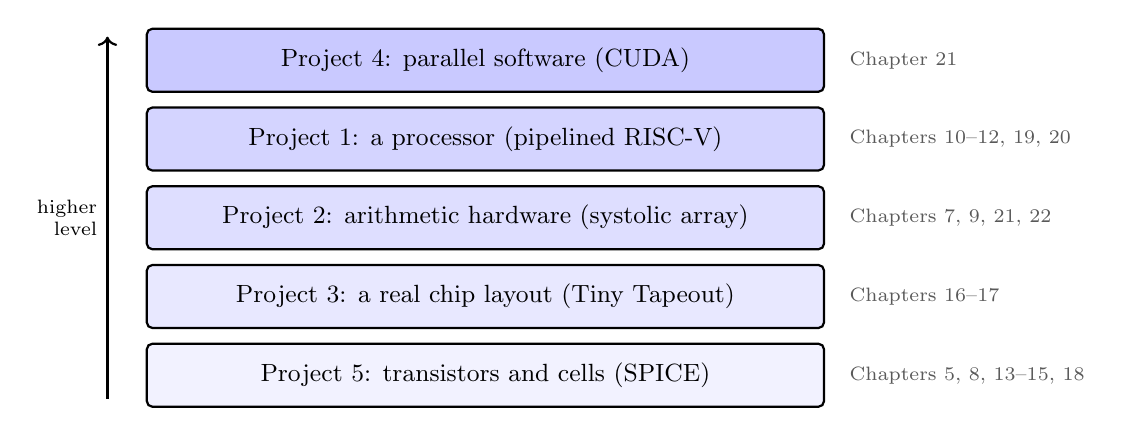
\begin{tikzpicture}[lvl/.style={draw,thick,rounded corners=2pt,minimum width=8.6cm,minimum height=0.8cm,font=\small}]
  \node[lvl,fill=blue!5]  at (0,0)   {Project 5: transistors and cells (SPICE)};
  \node[lvl,fill=blue!9]  at (0,1.0) {Project 3: a real chip layout (Tiny Tapeout)};
  \node[lvl,fill=blue!13] at (0,2.0) {Project 2: arithmetic hardware (systolic array)};
  \node[lvl,fill=blue!17] at (0,3.0) {Project 1: a processor (pipelined RISC-V)};
  \node[lvl,fill=blue!21] at (0,4.0) {Project 4: parallel software (CUDA)};
  \foreach \y/\t in {0/{Chapters 5, 8, 13--15, 18}, 1/{Chapters 16--17}, 2/{Chapters 7, 9, 21, 22}, 3/{Chapters 10--12, 19, 20}, 4/{Chapter 21}}
    \node[anchor=west,font=\scriptsize,gray!70!black] at (4.5,\y) {\t};
  \draw[->,thick] (-4.8,-0.3) -- node[left,font=\scriptsize,align=right]{higher\\level} (-4.8,4.3);
\end{tikzpicture}
\caption{The five core projects, from the lowest layer (transistors) to the highest (software), with the chapters each one exercises.}
\label{fig:projectstack}
\end{figure}

\begin{bigidea}
Three finished, verified, documented projects beat eight half-finished ones. The \textbf{minimum set} is Projects 1, 2 and 4, plus Project 3 whenever a Tiny Tapeout shuttle is open. Project 5 is small and directly strengthens your assessment knowledge, so do it early.
\end{bigidea}

All the tools below are free: Icarus Verilog or Verilator, cocotb, Yosys, nextpnr or the free edition of Vivado, OpenLane/OpenROAD, the SkyWater SKY130 process design kit, ngspice, Xschem, KiCad and the CUDA toolkit.

\section{Project 1: A pipelined RISC-V processor on an FPGA}

\textbf{Goal.} A processor you designed, verified, and ran a real program on.

\textbf{Build it in steps.}
\begin{enumerate}
  \item A single-cycle processor that executes the RV32I base instructions.
  \item Split it into the five stages of Chapter~\ref{ch:arch} (IF, ID, EX, MEM, WB). Add forwarding, the load-use stall and flushing on taken branches.
  \item Add a simple branch predictor (2-bit counters and a small branch target buffer) and measure how much it lowers CPI.
  \item Add a memory-mapped UART so a C program compiled with the RISC-V GCC toolchain can print text.
  \item Run it on an FPGA board. A low-cost Artix-7 board with the free Vivado edition, or a Lattice board with Yosys and nextpnr, both work.
\end{enumerate}

\textbf{Verify it.} Compare every retired instruction against a reference model (Spike, the official RISC-V simulator, or your own Python model) in a cocotb testbench. Run the official RISC-V architecture tests. Add SVA assertions for pipeline rules, and run random instruction sequences.

\textbf{Measure.} CPI on a small benchmark with and without branch prediction, maximum clock frequency from the timing report, and LUT, flip-flop and block-RAM usage.

\textbf{Shows:} computer architecture, SystemVerilog, verification. It also lets you answer ``what are the stages of a five-stage pipeline?'' with your own design. \textbf{Time:} about 10--12 weeks at 6--8 hours a week. \textbf{Stretch:} instruction and data caches, the M extension (hardware multiply and divide, which is computer arithmetic), interrupts.

\section{Project 2: A systolic-array matrix multiplier (a mini tensor core)}

\textbf{Goal.} Hardware for the operation that AI runs on, matrix multiplication (Chapter~\ref{ch:gpu}). This is the most NVIDIA-specific project in the plan.

A \term{systolic array} is a grid of small \term{processing elements} (PEs). Each PE multiplies the two numbers arriving from its neighbors, adds the product to a running sum, and passes the numbers on to the next PE in a steady rhythm, like a heartbeat (hence ``systolic''). Rows of one matrix flow in from the left and columns of the other flow in from the top (Figure~\ref{fig:systolic}). An $N \times N$ array performs $N^2$ multiply-adds every clock cycle.

\begin{figure}[h]
\centering
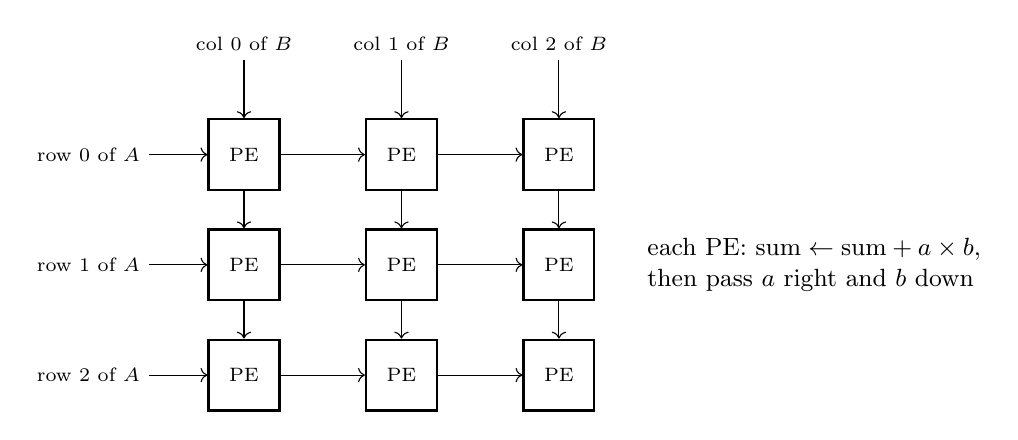
\begin{tikzpicture}[pe/.style={draw,thick,minimum size=0.9cm,font=\scriptsize}]
  \foreach \r in {0,1,2} \foreach \c in {0,1,2}
    \node[pe] (p\r\c) at (\c*2.0,-\r*1.4) {PE};
  \foreach \r in {0,1,2} {
    \draw[->] (-1.2,-\r*1.4) node[left,font=\scriptsize]{row \r\ of $A$} -- (p\r0.west);
    \draw[->] (p\r0.east) -- (p\r1.west); \draw[->] (p\r1.east) -- (p\r2.west);}
  \foreach \c in {0,1,2} {
    \draw[->] (\c*2.0,1.2) node[above,font=\scriptsize]{col \c\ of $B$} -- (p0\c.north);
    \draw[->] (p0\c.south) -- (p1\c.north); \draw[->] (p1\c.south) -- (p2\c.north);}
  \node[anchor=west,font=\small,align=left] at (5.0,-1.4) {each PE: $\text{sum} \leftarrow \text{sum} + a \times b$,\\then pass $a$ right and $b$ down};
\end{tikzpicture}
\caption{A $3 \times 3$ output-stationary systolic array. Each PE accumulates one element of the result matrix.}
\label{fig:systolic}
\end{figure}

\textbf{Build it in steps.}
\begin{enumerate}
  \item One PE: an INT8 $\times$ INT8 multiply feeding an INT32 accumulator.
  \item A $4 \times 4$ array with control for load, compute and drain.
  \item A host interface: a UART link from a PC, or memory-mapped registers on your Project~1 processor.
  \item A BF16 variant of the PE: multiply the significands, add the exponents, normalize, and round to nearest even. This is where computer arithmetic gets real.
\end{enumerate}

\textbf{Verify it.} In cocotb, compare the results bit for bit against NumPy for random matrices and corner cases such as $-128 \times -128$ and all-maximum inputs.

\textbf{Measure.} Multiply-adds per cycle, latency for an $N \times N$ product, maximum clock frequency and resources. Compare the achieved rate with the theoretical peak, PEs times clock frequency.

\textbf{Shows:} computer arithmetic, AI and parallel computing, VLSI, SystemVerilog. \textbf{Time:} about 6--8 weeks. \textbf{Stretch:} an $8 \times 8$ array, double buffering, INT4 or FP8 inputs.

\section{Project 3: Put a design on a real chip with Tiny Tapeout}

\textbf{Goal.} Take a design through the full physical design flow, and receive the manufactured chip.

\term{Tiny Tapeout} is an educational program that places many small designs side by side on one shared chip, so each person pays for only a small piece (a \term{tile}). It uses an open-source design flow and an open \term{process design kit} (PDK): the files that describe a factory's transistors and layout rules. Several shuttles (production runs) were offered during 2026. Dates and prices change, so check the Tiny Tapeout website for the next one.

\textbf{What to put on it.} Something small enough for a tile and its limited pins: a $2 \times 2$ version of Project~2, a Booth multiplier, or a compact state machine.

\textbf{Steps.}
\begin{enumerate}
  \item Write and verify the RTL with cocotb, using the program's project template.
  \item Run the automated flow to produce a layout (GDS file).
  \item Read every report: area, setup and hold slack, DRC and LVS results, and any antenna fixes. You can now explain the antenna rule (Section~\ref{sec:antenna}) from your own layout.
  \item Submit. When the chip arrives months later, test it and compare it with your simulation.
\end{enumerate}

\textbf{If no shuttle is open,} run OpenLane/OpenROAD on your own machine with the SKY130 PDK all the way to a layout. You will not get a chip, but you will have real physical design reports to discuss.

\textbf{Shows:} VLSI design, ASIC physical design and timing, CMOS. ``I taped out a chip'' is rare for a first- or second-year student. \textbf{Time:} about 4--6 weeks.

\section{Project 4: Optimizing matrix multiplication in CUDA}

\textbf{Goal.} Show that you can make a real NVIDIA GPU fast, and explain why each step helped, using Chapter~\ref{ch:gpu}.

\textbf{Steps.}
\begin{enumerate}
  \item A naive kernel: one thread computes one output element.
  \item Shared-memory tiling: each thread block loads tiles of the inputs once and reuses them.
  \item Register tiling: each thread computes a small block of outputs, reusing values held in registers.
  \item Vectorized loads, then (optionally) tensor cores through CUDA's WMMA interface with FP16 inputs.
  \item Compare each version with NVIDIA's cuBLAS library.
\end{enumerate}

\textbf{Measure.} GFLOP/s for each version at matrix sizes from 512 to 8192, as a percentage of cuBLAS. Profile with Nsight Compute (memory throughput, occupancy) and plot each version on a roofline chart. Then compare the GPU's multiply-adds per cycle with your Project~2 array.

\textbf{Hardware.} Any NVIDIA GPU: your own, a campus computing cluster, or a cloud notebook that offers one.

\textbf{Shows:} CUDA, parallel computing, AI. It fits the AI Developer Technology and performance teams especially well. \textbf{Time:} about 3--4 weeks.

\section{Project 5: Characterizing standard cells in SPICE}

\textbf{Goal.} See with your own simulations the transistor behavior this book describes. It is the fastest way to make the assessment's theory questions feel obvious.

Use ngspice and Xschem with the SKY130 PDK. Each experiment checks a chapter:
\begin{enumerate}
  \item An inverter's transfer curve, switching threshold and noise margins at several PMOS/NMOS size ratios (Chapter~\ref{ch:cmos}).
  \item An NMOS pass transistor's weak 1, and the swapped inverter from the assessment (Chapters~\ref{ch:mosfet} and~\ref{ch:cmos}).
  \item Delay versus fan-out, the FO4 delay, and a tapered buffer chain (Chapter~\ref{ch:delay}).
  \item Energy per transition versus supply voltage, to confirm the $CV^2$ law (Chapter~\ref{ch:power}).
  \item A temperature sweep from $-40$ to 125\,\textdegree C at normal and at low supply voltage, looking for temperature inversion (Chapter~\ref{ch:pvt}).
  \item A ring oscillator's frequency versus voltage and temperature.
  \item A 6T SRAM cell's read and write margins, and its butterfly curve (Chapter~\ref{ch:memory}).
\end{enumerate}

\textbf{Deliverable.} A short report with one plot per experiment, each compared with what this book predicts.

\textbf{Shows:} CMOS circuits, VLSI. \textbf{Time:} about 2--3 weeks.

\section{Track-specific options}

\paragraph{Project 6: GPU power and thermal characterization (power and infrastructure teams).} Log power draw, clock speed and temperature with \code{nvidia-smi} while running your Project~4 kernels at different sizes (and different clock settings, if your GPU allows it). Separate idle power from the extra power under load, fit the results to the $\alpha C V^2 f$-plus-leakage model of Chapter~\ref{ch:power}, estimate the energy per FLOP, and estimate the cooling system's thermal resistance from temperature rise versus power (Chapter~\ref{ch:heat}).

\paragraph{Project 7: Mechanical CAD (thermal and mechanical teams).} Design a heat sink, fan duct or enclosure in SolidWorks, Onshape or a similar tool. Size the fins and calculate the thermal resistance with Chapter~\ref{ch:heat}, then use the CAD tool's thermal simulation if it has one. Do the analysis in MATLAB or Python.

\paragraph{Project 8: A mini SIMT core (stretch goal).} Extend Project~1 into 4 to 8 lanes that execute one instruction stream on different data, with per-thread registers, an active mask for divergent branches, and a scheduler that switches between two warps. Run vector-add and matrix-add kernels and compare throughput with the scalar core. Open-source teaching designs such as tiny-gpu and the Vortex RISC-V GPGPU are worth studying for ideas, but write your own; interviewers will ask about every design decision.

\section{When to do what}

The month-by-month plan in Appendix~\ref{app:plan} fits the projects in alongside the reading. In short: Project~5 in January and March, Project~1 from February to April, Project~2 in May and June, Project~3 whenever a shuttle opens, Project~4 in July, and the track-specific projects in August if you want them.

\section{Making the projects count}

\paragraph{Each project's repository needs:}
\begin{itemize}
  \item[$\square$] a README with the specification, a block diagram and known limitations;
  \item[$\square$] one command that runs all the tests, ideally also run automatically on every push;
  \item[$\square$] a results table (clock frequency, resources, CPI, GFLOP/s or whatever the project measures);
  \item[$\square$] waveforms or plots that show the design working.
\end{itemize}

\paragraph{Writing resume bullets.} Each bullet says what you built, how you verified it, and a number you measured:

\begin{remember}
\begin{itemize}
  \item \textit{Designed a 5-stage pipelined RV32I processor in SystemVerilog with forwarding and branch prediction; verified against a reference model with cocotb, passing X of Y architecture tests; ran at Z\,MHz on an Artix-7 FPGA using N LUTs.}
  \item \textit{Built a 4$\times$4 INT8 systolic-array matrix multiplier, bit-exact against NumPy over X random tests; sustained Y multiply-adds per cycle at Z\,MHz.}
  \item \textit{Optimized CUDA matrix multiplication from X to Y GFLOP/s (Z\% of cuBLAS) with shared-memory and register tiling; analyzed each version with Nsight Compute and a roofline model.}
\end{itemize}
Replace X, Y, Z and N with numbers you actually measured. Never write a number you did not measure.
\end{remember}

\paragraph{The rest of the resume.} The posting requires your expected graduation month and year, and asks for clubs, leadership or extracurricular projects. A hardware-related club (IEEE, robotics, a solar-car or Formula team) or a hackathon project counts.

\paragraph{Be ready to defend every line.} Interviewers pick a project and dig: why these widths, what limits the clock frequency, what happens under backpressure, what the hardest bug was. Rehearse a two-minute explanation of each project, using Book 3's project deep-dive drill.

\chapter{Sources}
\label{app:sources}

The job-description details in Appendix~\ref{app:projects} come from NVIDIA's own postings, listed at the end of this appendix. The ``Seen on the assessment'' boxes in this book draw on two kinds of source: the questions from an actual Ignite hardware assessment that motivated this book, and anonymous candidate reports gathered online in October 2026. The reports are unverified, some describe other NVIDIA hardware roles rather than Ignite, and formats change between years. Glassdoor pages could only be read through search-engine summaries. Treat every reported detail as a hint about the \emph{kind} of question to expect, not as a promise.

\section*{From the assessment that motivated this book}
A linked-list coding problem; the advantage of a flip-flop over a latch; an OR gate from a 2:1 mux; the inverter with swapped transistors; dynamic power when frequency and voltage double; carrier mobility and wire resistance versus temperature; and a true/false question on the antenna rule.

\section*{Candidate reports and preparation sites}
\begin{itemize}\small
  \item Glassdoor, NVIDIA IGNITE Intern interview questions:\\ \url{https://www.glassdoor.com/Interview/NVIDIA-IGNITE-Intern-Interview-Questions-EI_IE7633.0,6_KO7,20.htm}
  \item Glassdoor, NVIDIA Hardware Intern interview questions:\\ \url{https://www.glassdoor.com/Interview/NVIDIA-Hardware-Intern-Interview-Questions-EI_IE7633.0,6_KO7,22.htm}
  \item Glassdoor, NVIDIA interview review (hardware multiple choice on transistors, circuits and heat sinks):\\ \url{https://www.glassdoor.com/Interview/NVIDIA-Interview-E7633-RVW104894219.htm}
  \item Glassdoor, NVIDIA clock-divider interview question:\\ \url{https://www.glassdoor.com/Interview/One-of-the-questions-is-about-clock-divider-and-the-interviewer-asked-a-lot-different-questions-related-to-divider-design-QTN_418519.htm}
  \item InterviewFox, NVIDIA Ignite OA on HackerRank (format, coding problems, GND and FIFO topics):\\ \url{https://interviewfox.ai/interview-questions/nvidia-oa-hackerrank-questions/}
  \item Jointaro, NVIDIA Ignite software engineer interview experience (November 2025):\\ \url{https://www.jointaro.com/interviews/companies/nvidia/experiences/software-engineer-ignite-united-states-november-4-2025-no-offer-neutral-c2955f45/}
  \item PracHub, NVIDIA Ignite Internship 2027 guide:\\ \url{https://prachub.com/resources/nvidia-ignite-internship-2027-eligibility-interview-process-and-preparation}
  \item Nora HQ, NVIDIA Ignite intern interview guide:\\ \url{https://interview.norahq.com/interview-guides/nvidia-ignite-intern-interview-guide-2025}
  \item AnitaB.org job board, NVIDIA 2025 Ignite Internships: Hardware Engineering (eligibility, skills, roles):\\ \url{https://jobs.anitab.org/companies/nvidia/jobs/40510638-nvidia-2025-ignite-internships-hardware-engineering}
  \item VLSI4Freshers, NVIDIA ASIC design test questions (power scaling, FIFO depth, caches, NMOS networks, aptitude):\\ \url{https://www.vlsi4freshers.com/2022/02/nvidia-asic-design-interview-questions.html}
  \item VLSI4Freshers, NVIDIA ASIC verification test questions (counters, XOR chains, reset glitch filtering, Verilog, AMAT, C output):\\ \url{https://www.vlsi4freshers.com/2023/03/nvidia-asic-verification-interview-questions.html}
  \item Snubber, NVIDIA engineering interview questions (practice problems on decoupling, heat sinks, reflections, ADCs):\\ \url{https://snubber.ai/blog/nvidia-interview-questions}
  \item Voltage Learning, NVIDIA internship interview process:\\ \url{https://voltagelearning.com/blog/nvidia-internship-interview-process}
  \item LeakCode, NVIDIA online assessment reports:\\ \url{https://leakcode.dev/company/nvidia/oa/2026}
  \item Lodely, NVIDIA online assessment overview:\\ \url{https://www.lodely.com/companies/nvidia/online-assessment}
\end{itemize}

\section*{Job postings and project resources (Appendix~\ref{app:projects})}
\begin{itemize}\small
  \item NVIDIA 2027 Ignite Internships: Hardware Engineering (eligibility, requirements, ways to stand out, teams, dates), AnitaB.org copy:\\ \url{https://jobs.anitab.org/companies/nvidia/jobs/95889112-nvidia-2027-ignite-internships-hardware-engineering}
  \item The same posting on NVIDIA's careers site:\\ \url{https://jobs.nvidia.com/careers/job/893397961094}
  \item NVIDIA 2026 Ignite Internships: Hardware Engineering (application window October 6--19, 2025):\\ \url{https://jobs.anitab.org/companies/nvidia/jobs/59992858-nvidia-2026-ignite-internships-hardware-engineering}
  \item NVIDIA 2027 Internships: Hardware ASIC Design:\\ \url{https://jobs.nvidia.com/careers/job/893397025803}
  \item NVIDIA ASIC Design and Verification Intern, SOC, 2027:\\ \url{https://nvidia.wd5.myworkdayjobs.com/en-US/NVIDIAExternalCareerSite/job/ASIC-Design-and-Verification-Intern--SOC---2027_JR2024860}
  \item NVIDIA 2026 Internships: Hardware Physical Design / VLSI:\\ \url{https://jobs.nvidia.com/careers/job/893384237248}
  \item Extern, NVIDIA Ignite 2027 program guide (application dates):\\ \url{https://www.extern.com/post/nvidia-ignite-program-guide}
  \item Tiny Tapeout, list of shuttles:\\ \url{https://tinytapeout.com/tags/shuttle/}
  \item tiny-gpu, an educational GPU in Verilog:\\ \url{https://hellogithub.com/en/repository/adam-maj/tiny-gpu}
  \item Vortex, an open-source RISC-V GPGPU from Georgia Tech:\\ \url{https://github.com/vortexgpgpu/vortex}
\end{itemize}


\end{document}
